% =====================================================================
% Austin's Working Musicians: Earnings, Venues, and Public Support
%
% Build:  make            (from inside 05_report/)
% Engine: xelatex via latexmk
%
% This file is a shell. The prose lives in sections/, the numbers come from
% canonical_numbers.tex (generated by 03_analysis/src/build_numbers.py from the
% analysis modules), and the figures come from 04_figures/ (generated by the
% scripts in 03_analysis/src/). Nothing here is typed by hand twice.
%
% Every path is relative, so the project folder can be zipped and moved.
% =====================================================================
\documentclass[10pt]{article}
\usepackage{style/austinmusic}

% Figures are generated into 04_figures/ by the analysis scripts.
\graphicspath{{../04_figures/}}

% Generated macros for every number quoted in the prose. If this file is
% missing, run `make numbers`.
\IfFileExists{canonical_numbers.tex}{% canonical_numbers.tex - GENERATED FILE, DO NOT EDIT BY HAND.
% Produced by 03_analysis/stata/build_numbers.do from the module ledgers.
% Every quantity quoted in the report is defined here, so the prose and
% the analysis cannot drift apart.
% Generated from 1177 registered numbers.

% ---- census (139 numbers) ------------------------------
% census_also_presents_gigs: Share of music creatives who also present or promote gigs, casually or professionally, of 1151 who answered. THIS IS NOT WORK OUTSIDE MUSIC:...
\newcommand{\NCensusAlsoPresentsGigs}{47.2\%\xspace}
% census_caveat_2014comparison: Where the 2014 census asked a comparable question, the comparison runs between two different self-selected samples eight years apart, with r...
\newcommand{\NCensusCaveatTwoZeroOneFourcomparison}{2014 comparisons are directional\xspace}
% census_caveat_nodollarincome: The instrument contains no dollar-denominated income question of any kind - annual, monthly or per gig. The share-of-income scale used in se...
\newcommand{\NCensusCaveatNodollarincome}{no dollar income variable\xspace}
% census_caveat_nofollowup: One cross-section with no comparable follow-up. Austin appears in the Sound Music Cities 2023-24 cohort roster but published no later report...
\newcommand{\NCensusCaveatNofollowup}{single 2022 snapshot\xspace}
% census_caveat_notacs: Do not set these percentages beside the ACS, PUMS, OEWS or QCEW figures elsewhere in this report as though they measure the same population....
\newcommand{\NCensusCaveatNotacs}{not comparable with ACS or PUMS\xspace}
% census_caveat_noweights: The release carries no design or post-stratification weights, so no statistic here is a population estimate, and no standard error or margin...
\newcommand{\NCensusCaveatNoweights}{no survey weights\xspace}
% census_caveat_rowcount: The published microdata file carries 2,227 respondent rows; the Summary Report and Data Appendix headline 2,260. The 33-row difference is un...
\newcommand{\NCensusCaveatRowcount}{2,227 rows, not 2,260\xspace}
% census_caveat_selfselected: The 2022 Greater Austin Music Census recruited online through community partners between 15 July and 12 September 2022. It is not a probabil...
\newcommand{\NCensusCaveatSelfselected}{self-selected convenience sample\xspace}
% census_caveat_slide41: Two published sources disagree about which income source goes with which value. The microdata, the Socrata column dictionary for dataset an3...
\newcommand{\NCensusCaveatSlideFourOne}{published slide 41 mislabels four bars\xspace}
% census_closures_property_share: Share of the 36 dated Austin venue closures in the 30_venues tracking panel attributed to a real-estate cause - sale of the property, a rent...
\newcommand{\NCensusClosuresPropertyShare}{36.1\%\xspace}
% census_gig_guarantee_mean: Mean self-reported percent of gigs paying a base guarantee rather than a door or bar percentage, 1086 creatives. Replicates the published 54...
\newcommand{\NCensusGigGuaranteeMean}{54.3\%\xspace}
% census_gigs_any: Share reporting at least one paid local performance a month, of 1086 who answered. 2022 Greater Austin Music Census, self-selected online co...
\newcommand{\NCensusGigsAny}{86.0\%\xspace}
% census_gigs_by_experience_chi2: Test of independence between the monthly paid-gig band and years of experience among music creatives. Not distinguishable: gig volume looks ...
\newcommand{\NCensusGigsByExperienceChiTwo}{chi-squared(15) = 20.0, p = 0.173\xspace}
% census_gigs_item_from_creatives: Share of the gig-volume respondents whose primary sector is Music Creative. Because it is essentially 100 percent, a sector cross-tabulation...
\newcommand{\NCensusGigsItemFromCreatives}{99.8\%\xspace}
% census_gigs_over10: Share reporting more than 10 paid local performances a month, of 1086 who answered. A working-musician week is four or more gigs; this is th...
\newcommand{\NCensusGigsOverOneZero}{8.9\%\xspace}
% census_gigs_over3: Share reporting more than 3 paid local performances a month - the 4-to-6, 7-to-10, 11-to-15 and 16-or-more bands - of 1086 who answered. Rep...
\newcommand{\NCensusGigsOverThree}{34.9\%\xspace}
% census_gigs_over3_restored: Share reporting more than 3 paid local performances a month among the 745 creatives who also said their music work has returned to pre-pande...
\newcommand{\NCensusGigsOverThreeRestored}{37.9\%\xspace}
% census_gigs_zero: Share of music creatives reporting zero paid local performances a month, of 1086 who answered. Replicates the published 14 percent (Data App...
\newcommand{\NCensusGigsZero}{14.0\%\xspace}
% census_incshare_allmost_live_performance_local: Share of music creatives saying ALL or MOST of their music income comes from Live performance, local. Denominator 1119 creatives who answere...
\newcommand{\NCensusIncshareAllmostLivePerformanceLocal}{50.8\%\xspace}
% census_incshare_allmost_live_performance_touring: Share of music creatives saying ALL or MOST of their music income comes from Live performance, touring. Denominator 948 creatives who answer...
\newcommand{\NCensusIncshareAllmostLivePerformanceTouring}{12.0\%\xspace}
% census_incshare_allmost_merchandise: Share of music creatives saying ALL or MOST of their music income comes from Merchandise. Denominator 839 creatives who answered this item. ...
\newcommand{\NCensusIncshareAllmostMerchandise}{3.9\%\xspace}
% census_incshare_allmost_recordings_and_royalties: Share of music creatives saying ALL or MOST of their music income comes from Recordings and royalties. Denominator 928 creatives who answere...
\newcommand{\NCensusIncshareAllmostRecordingsAndRoyalties}{5.6\%\xspace}
% census_incshare_allmost_songwriting_and_mechanicals: Share of music creatives saying ALL or MOST of their music income comes from Songwriting and mechanicals. Denominator 859 creatives who answ...
\newcommand{\NCensusIncshareAllmostSongwritingAndMechanicals}{3.8\%\xspace}
% census_incshare_allmost_studio_and_session_work: Share of music creatives saying ALL or MOST of their music income comes from Studio and session work. Denominator 929 creatives who answered...
\newcommand{\NCensusIncshareAllmostStudioAndSessionWork}{7.9\%\xspace}
% census_incshare_allmost_teaching: Share of music creatives saying ALL or MOST of their music income comes from Teaching. Denominator 903 creatives who answered this item. Wit...
\newcommand{\NCensusIncshareAllmostTeaching}{13.6\%\xspace}
% census_incshare_any_live_performance_local: Share of music creatives reporting any income at all from Live performance, local - all, most, some or very little, excluding none. Denomina...
\newcommand{\NCensusIncshareAnyLivePerformanceLocal}{92.4\%\xspace}
% census_incshare_any_live_performance_touring: Share of music creatives reporting any income at all from Live performance, touring - all, most, some or very little, excluding none. Denomi...
\newcommand{\NCensusIncshareAnyLivePerformanceTouring}{75.3\%\xspace}
% census_incshare_any_merchandise: Share of music creatives reporting any income at all from Merchandise - all, most, some or very little, excluding none. Denominator 839. Sou...
\newcommand{\NCensusIncshareAnyMerchandise}{56.1\%\xspace}
% census_incshare_any_recordings_and_royalties: Share of music creatives reporting any income at all from Recordings and royalties - all, most, some or very little, excluding none. Denomin...
\newcommand{\NCensusIncshareAnyRecordingsAndRoyalties}{70.7\%\xspace}
% census_incshare_any_songwriting_and_mechanicals: Share of music creatives reporting any income at all from Songwriting and mechanicals - all, most, some or very little, excluding none. Deno...
\newcommand{\NCensusIncshareAnySongwritingAndMechanicals}{51.0\%\xspace}
% census_incshare_any_studio_and_session_work: Share of music creatives reporting any income at all from Studio and session work - all, most, some or very little, excluding none. Denomina...
\newcommand{\NCensusIncshareAnyStudioAndSessionWork}{57.8\%\xspace}
% census_incshare_any_teaching: Share of music creatives reporting any income at all from Teaching - all, most, some or very little, excluding none. Denominator 903. Source...
\newcommand{\NCensusIncshareAnyTeaching}{41.0\%\xspace}
% census_intend_continue_definitely: Share answering DEFINITELY yes to continuing music work, 1900 respondents. The published 89 percent folds in maybe yes; this is the firm par...
\newcommand{\NCensusIntendContinueDefinitely}{74.7\%\xspace}
% census_intend_continue_music: Share intending to continue their music work over the next three years - definitely yes plus maybe yes - 1900 respondents. Verifies the publ...
\newcommand{\NCensusIntendContinueMusic}{88.8\%\xspace}
% census_intend_stay_austin: Share intending to still live in greater Austin in three years - definitely yes plus maybe yes - 1900 respondents. Verifies the published 64...
\newcommand{\NCensusIntendStayAustin}{64.1\%\xspace}
% census_intend_stay_definitely: Share answering DEFINITELY yes to still living in greater Austin in three years, 1900 respondents. Below half. 2022 Greater Austin Music Cen...
\newcommand{\NCensusIntendStayDefinitely}{44.2\%\xspace}
% census_logit_n: Estimation sample for the retention logit that includes housing tenure and insurance. It is smaller than the 1,900 who answered the retentio...
\newcommand{\NCensusLogitN}{1,607\xspace}
% census_logit_renter_or: Odds ratio on renting, relative to owning, in a logit of intending to stay in greater Austin on primary sector, years of experience, housing...
\newcommand{\NCensusLogitRenterOr}{0.39\xspace}
% census_miles_mean: Mean self-reported distance from downtown Austin, 2150 respondents who answered. Matches the published 10.6-mile average. 2022 Greater Austi...
\newcommand{\NCensusMilesMean}{10.6 miles\xspace}
% census_miles_median: Median self-reported distance from downtown Austin, 2150 respondents. Matches the published 8-mile median. 2022 Greater Austin Music Census,...
\newcommand{\NCensusMilesMedian}{8 miles\xspace}
% census_n_city_item: Respondents who answered the City of Austin residency item. 2022 Greater Austin Music Census, self-selected online convenience sample fielde...
\newcommand{\NCensusNCityItem}{2,149\xspace}
% census_n_gigs_item: Music creatives who answered the paid-local-performances-per-month item. 2022 Greater Austin Music Census, self-selected online convenience ...
\newcommand{\NCensusNGigsItem}{1,086\xspace}
% census_n_independent_promoters: Presenters identifying as independent promoters rather than room operators. Below the 50-record floor, so no statistic is published for this...
\newcommand{\NCensusNIndependentPromoters}{43\xspace}
% census_n_presenters_ranking: Respondents who completed the nine-item ranking of business pressures. Above the 50-record floor in aggregate, so it is published, but it is...
\newcommand{\NCensusNPresentersRanking}{177\xspace}
% census_n_respondents: Respondent records in the published microdata file. The Summary Report headline count is 2,260; the microdata release carries 2,227 rows, 33...
\newcommand{\NCensusNRespondents}{2,227\xspace}
% census_n_sector_creative: Respondents whose primary music ecosystem sector is Music Creative. The sector item itself was answered by 2128 of 2227. 2022 Greater Austin...
\newcommand{\NCensusNSectorCreative}{1,462\xspace}
% census_n_sector_exited: Selected None of these - Exit the Census, which terminated the questionnaire. They remain in the 2,227-row file and in any all-respondent de...
\newcommand{\NCensusNSectorExited}{69\xspace}
% census_n_sector_industry: Primary sector Music Industry, of 2128 who answered the sector item. 2022 Greater Austin Music Census, self-selected online convenience samp...
\newcommand{\NCensusNSectorIndustry}{489\xspace}
% census_n_sector_presenter: Primary sector Music Venue or Presenter, of 2128 who answered the sector item. This is the smallest of the three role groups and it caps eve...
\newcommand{\NCensusNSectorPresenter}{108\xspace}
% census_n_venue_operators: Presenters reporting a numeric legal capacity band, that is, operators of a physical room. 2022 Greater Austin Music Census, self-selected o...
\newcommand{\NCensusNVenueOperators}{131\xspace}
% census_no_outside_work_item: The census DID ask about work outside music - Data Appendix slide 15 reports 38 percent in a non-creative industry, 24 percent in another cr...
\newcommand{\NCensusNoOutsideWorkItem}{not in the microdata\xspace}
% census_pct_city_of_austin: Share who are City of Austin residents: 1567 of the 2149 who answered the item. On the full 2,227-row denominator it is 70.4 percent, becaus...
\newcommand{\NCensusPctCityOfAustin}{72.9\%\xspace}
% census_pct_travis: Share living in Travis County: 1785 of 2227. County is the only item with complete response, which suggests it gated entry to the survey. Th...
\newcommand{\NCensusPctTravis}{80.2\%\xspace}
% census_presents_by_experience_chi2: Test of independence between also presenting or promoting gigs and years of experience. Not distinguishable. Association only; the p-value a...
\newcommand{\NCensusPresentsByExperienceChiTwo}{chi-squared(3) = 0.7, p = 0.871\xspace}
% census_presents_by_gigs_chi2: Test of independence between also presenting or promoting gigs and the monthly paid-gig band. Creatives who play more also promote more. Ass...
\newcommand{\NCensusPresentsByGigsChiTwo}{chi-squared(5) = 15.1, p = 0.010\xspace}
% census_pressure_first_building_operations_and_upkeep: Share of the 177 responding presenters who ranked Building operations and upkeep their single greatest business pressure. The nine first-pla...
\newcommand{\NCensusPressureFirstBuildingOperationsAndUpkeep}{7.9\%\xspace}
% census_pressure_first_changing_audience_behavior: Share of the 177 responding presenters who ranked Changing audience behavior their single greatest business pressure. The nine first-place s...
\newcommand{\NCensusPressureFirstChangingAudienceBehavior}{10.7\%\xspace}
% census_pressure_first_labor_cost_and_retention: Share of the 177 responding presenters who ranked Labor cost and retention their single greatest business pressure. The nine first-place sha...
\newcommand{\NCensusPressureFirstLaborCostAndRetention}{11.3\%\xspace}
% census_pressure_first_marketing: Share of the 177 responding presenters who ranked Marketing their single greatest business pressure. The nine first-place shares sum to 100 ...
\newcommand{\NCensusPressureFirstMarketing}{4.0\%\xspace}
% census_pressure_first_neighborhood_redevelopment: Share of the 177 responding presenters who ranked Neighborhood redevelopment their single greatest business pressure. The nine first-place s...
\newcommand{\NCensusPressureFirstNeighborhoodRedevelopment}{8.5\%\xspace}
% census_pressure_first_ordinances_and_permitting: Share of the 177 responding presenters who ranked Ordinances and permitting their single greatest business pressure. The nine first-place sh...
\newcommand{\NCensusPressureFirstOrdinancesAndPermitting}{12.4\%\xspace}
% census_pressure_first_property_tax: Share of the 177 responding presenters who ranked Property tax their single greatest business pressure. The nine first-place shares sum to 1...
\newcommand{\NCensusPressureFirstPropertyTax}{20.3\%\xspace}
% census_pressure_first_talent_costs: Share of the 177 responding presenters who ranked Talent costs their single greatest business pressure. The nine first-place shares sum to 1...
\newcommand{\NCensusPressureFirstTalentCosts}{13.6\%\xspace}
% census_pressure_first_unpredictable_operating_costs: Share of the 177 responding presenters who ranked Unpredictable operating costs their single greatest business pressure. The nine first-plac...
\newcommand{\NCensusPressureFirstUnpredictableOperatingCosts}{11.3\%\xspace}
% census_pressure_top3_building_operations_and_upkeep: Share of the 177 responding presenters who ranked Building operations and upkeep among their three greatest business pressures. Nine items, ...
\newcommand{\NCensusPressureTopThreeBuildingOperationsAndUpkeep}{31.6\%\xspace}
% census_pressure_top3_changing_audience_behavior: Share of the 177 responding presenters who ranked Changing audience behavior among their three greatest business pressures. Nine items, each...
\newcommand{\NCensusPressureTopThreeChangingAudienceBehavior}{31.6\%\xspace}
% census_pressure_top3_labor_cost_and_retention: Share of the 177 responding presenters who ranked Labor cost and retention among their three greatest business pressures. Nine items, each r...
\newcommand{\NCensusPressureTopThreeLaborCostAndRetention}{35.6\%\xspace}
% census_pressure_top3_marketing: Share of the 177 responding presenters who ranked Marketing among their three greatest business pressures. Nine items, each respondent ranke...
\newcommand{\NCensusPressureTopThreeMarketing}{19.2\%\xspace}
% census_pressure_top3_neighborhood_redevelopment: Share of the 177 responding presenters who ranked Neighborhood redevelopment among their three greatest business pressures. Nine items, each...
\newcommand{\NCensusPressureTopThreeNeighborhoodRedevelopment}{32.2\%\xspace}
% census_pressure_top3_ordinances_and_permitting: Share of the 177 responding presenters who ranked Ordinances and permitting among their three greatest business pressures. Nine items, each ...
\newcommand{\NCensusPressureTopThreeOrdinancesAndPermitting}{33.3\%\xspace}
% census_pressure_top3_property_tax: Share of the 177 responding presenters who ranked Property tax among their three greatest business pressures. Nine items, each respondent ra...
\newcommand{\NCensusPressureTopThreePropertyTax}{44.1\%\xspace}
% census_pressure_top3_talent_costs: Share of the 177 responding presenters who ranked Talent costs among their three greatest business pressures. Nine items, each respondent ra...
\newcommand{\NCensusPressureTopThreeTalentCosts}{38.4\%\xspace}
% census_pressure_top3_unpredictable_operating_costs: Share of the 177 responding presenters who ranked Unpredictable operating costs among their three greatest business pressures. Nine items, e...
\newcommand{\NCensusPressureTopThreeUnpredictableOperatingCosts}{33.9\%\xspace}
% census_retention_denom: Respondents answering the three-year intent items. Both items have exactly the same 1900 answers out of 2,227, so the 89 and the 64 rest on ...
\newcommand{\NCensusRetentionDenom}{1,900\xspace}
% census_retention_gap: Gap between the share intending to continue in music and the share intending to stay in greater Austin, on the same 1900 respondents. The Su...
\newcommand{\NCensusRetentionGap}{24.7 points\xspace}
% census_spend_complete_n: Music creatives who gave a figure for all eight spending categories. This is the only base on which a per-respondent total is complete, and ...
\newcommand{\NCensusSpendCompleteN}{501\xspace}
% census_spend_mean_accounting_and_legal: Mean annual spending on Accounting and legal, 2025 dollars, 611 music creatives who answered this category. 2022 Greater Austin Music Census...
\newcommand{\NCensusSpendMeanAccountingAndLegal}{\textdollar{}670\xspace}
% census_spend_mean_gear_and_rentals: Mean annual spending on Gear and rentals, 2025 dollars, 737 music creatives who answered this category. 2022 Greater Austin Music Census, se...
\newcommand{\NCensusSpendMeanGearAndRentals}{\textdollar{}1,522\xspace}
% census_spend_mean_merchandise: Mean annual spending on Merchandise, 2025 dollars, 625 music creatives who answered this category. 2022 Greater Austin Music Census, self-se...
\newcommand{\NCensusSpendMeanMerchandise}{\textdollar{}1,029\xspace}
% census_spend_mean_new_recordings: Mean annual spending on New recordings, 2025 dollars, 728 music creatives who answered this category. 2022 Greater Austin Music Census, self...
\newcommand{\NCensusSpendMeanNewRecordings}{\textdollar{}3,917\xspace}
% census_spend_mean_publicity_and_promotion: Mean annual spending on Publicity and promotion, 2025 dollars, 690 music creatives who answered this category. 2022 Greater Austin Music Cen...
\newcommand{\NCensusSpendMeanPublicityAndPromotion}{\textdollar{}1,506\xspace}
% census_spend_mean_rehearsal_or_work_space: Mean annual spending on Rehearsal or work space, 2025 dollars, 646 music creatives who answered this category. 2022 Greater Austin Music Cen...
\newcommand{\NCensusSpendMeanRehearsalOrWorkSpace}{\textdollar{}1,536\xspace}
% census_spend_mean_supplies: Mean annual spending on Supplies, 2025 dollars, 742 music creatives who answered this category. 2022 Greater Austin Music Census, self-selec...
\newcommand{\NCensusSpendMeanSupplies}{\textdollar{}960\xspace}
% census_spend_mean_web_and_social_media: Mean annual spending on Web and social media, 2025 dollars, 709 music creatives who answered this category. 2022 Greater Austin Music Census...
\newcommand{\NCensusSpendMeanWebAndSocialMedia}{\textdollar{}528\xspace}
% census_spend_median_accounting_and_legal: Median annual spending on Accounting and legal, 2025 dollars, 611 music creatives who answered this category. 2022 Greater Austin Music Cens...
\newcommand{\NCensusSpendMedianAccountingAndLegal}{\textdollar{}0\xspace}
% census_spend_median_gear_and_rentals: Median annual spending on Gear and rentals, 2025 dollars, 737 music creatives who answered this category. 2022 Greater Austin Music Census, ...
\newcommand{\NCensusSpendMedianGearAndRentals}{\textdollar{}550\xspace}
% census_spend_median_merchandise: Median annual spending on Merchandise, 2025 dollars, 625 music creatives who answered this category. 2022 Greater Austin Music Census, self-...
\newcommand{\NCensusSpendMedianMerchandise}{\textdollar{}330\xspace}
% census_spend_median_new_recordings: Median annual spending on New recordings, 2025 dollars, 728 music creatives who answered this category. 2022 Greater Austin Music Census, se...
\newcommand{\NCensusSpendMedianNewRecordings}{\textdollar{}1,651\xspace}
% census_spend_median_publicity_and_promotion: Median annual spending on Publicity and promotion, 2025 dollars, 690 music creatives who answered this category. 2022 Greater Austin Music C...
\newcommand{\NCensusSpendMedianPublicityAndPromotion}{\textdollar{}330\xspace}
% census_spend_median_rehearsal_or_work_space: Median annual spending on Rehearsal or work space, 2025 dollars, 646 music creatives who answered this category. 2022 Greater Austin Music C...
\newcommand{\NCensusSpendMedianRehearsalOrWorkSpace}{\textdollar{}275\xspace}
% census_spend_median_supplies: Median annual spending on Supplies, 2025 dollars, 742 music creatives who answered this category. 2022 Greater Austin Music Census, self-sel...
\newcommand{\NCensusSpendMedianSupplies}{\textdollar{}550\xspace}
% census_spend_median_web_and_social_media: Median annual spending on Web and social media, 2025 dollars, 709 music creatives who answered this category. 2022 Greater Austin Music Cens...
\newcommand{\NCensusSpendMedianWebAndSocialMedia}{\textdollar{}220\xspace}
% census_spend_share_local: Mean self-reported percent of annual music business spending that goes to providers inside the Austin area, 888 creatives; median 70 percent...
\newcommand{\NCensusSpendShareLocal}{60.5\%\xspace}
% census_spend_sumofmeans_2022: Sum of the eight category MEANS, each on its own base of between 611 and 742 creatives. This reproduces the published average annual spend o...
\newcommand{\NCensusSpendSumofmeansTwoZeroTwoTwo}{\textdollar{}10,599\xspace}
% census_spend_sumofmeans_2025: The same sum of eight category means, inflated from 2022 to 2025 dollars with the CPI-U annual factor from out/cpi_annual.dta. 2022 Greater ...
\newcommand{\NCensusSpendSumofmeansTwoZeroTwoFive}{\textdollar{}11,667\xspace}
% census_spend_total_mean: MEAN total annual spending on their own music work, 2025 dollars, all eight categories, 501 creatives who answered every category. The publi...
\newcommand{\NCensusSpendTotalMean}{\textdollar{}10,288\xspace}
% census_spend_total_mean_anyitem: MEAN total annual spending, 2025 dollars, over the 873 creatives who answered at least one category, treating unanswered categories as zero....
\newcommand{\NCensusSpendTotalMeanAnyitem}{\textdollar{}9,328\xspace}
% census_spend_total_median: MEDIAN total annual spending on their own music work, 2025 dollars, 501 creatives who answered every category. It is roughly half the mean, ...
\newcommand{\NCensusSpendTotalMedian}{\textdollar{}5,394\xspace}
% census_spend_total_median_anyitem: MEDIAN total annual spending, 2025 dollars, 873 creatives who answered at least one category, blanks treated as zero. Lower bound, same reas...
\newcommand{\NCensusSpendTotalMedianAnyitem}{\textdollar{}4,678\xspace}
% census_spend_total_p25: 25th percentile of total annual spending, 2025 dollars, 501 creatives answering all eight categories. 2022 Greater Austin Music Census, self...
\newcommand{\NCensusSpendTotalPTwoFive}{\textdollar{}1,816\xspace}
% census_spend_total_p75: 75th percentile of total annual spending, 2025 dollars, 501 creatives answering all eight categories. 2022 Greater Austin Music Census, self...
\newcommand{\NCensusSpendTotalPSevenFive}{\textdollar{}11,834\xspace}
% census_spend_total_p90: 90th percentile of total annual spending, 2025 dollars, 501 creatives answering all eight categories. The gap between this and the median is...
\newcommand{\NCensusSpendTotalPNineZero}{\textdollar{}22,016\xspace}
% census_spend_vs_nes_receipts: Census Bureau Nonemployer Statistics reports average gross receipts of roughly 32,962 dollars for NAICS 7115 establishments, BEFORE any expe...
\newcommand{\NCensusSpendVsNesReceipts}{the missing cost side of a receipts figure\xspace}
% census_stay_health_insurance_has_health_insurance: Share intending to still live in greater Austin in three years among the 1,390 respondents in the group Has health insurance (breakout varia...
\newcommand{\NCensusStayHealthInsuranceHasHealthInsurance}{66.1\%\xspace}
% census_stay_health_insurance_no_health_insurance: Share intending to still live in greater Austin in three years among the 254 respondents in the group No health insurance (breakout variable...
\newcommand{\NCensusStayHealthInsuranceNoHealthInsurance}{53.1\%\xspace}
% census_stay_housing_tenure_homeowner: Share intending to still live in greater Austin in three years among the 758 respondents in the group Homeowner (breakout variable: Housing ...
\newcommand{\NCensusStayHousingTenureHomeowner}{75.5\%\xspace}
% census_stay_housing_tenure_other_or_unstable_housing: Share intending to still live in greater Austin in three years among the 174 respondents in the group Other or unstable housing (breakout va...
\newcommand{\NCensusStayHousingTenureOtherOrUnstableHousing}{63.2\%\xspace}
% census_stay_housing_tenure_renter: Share intending to still live in greater Austin in three years among the 688 respondents in the group Renter (breakout variable: Housing ten...
\newcommand{\NCensusStayHousingTenureRenter}{52.3\%\xspace}
% census_stay_music_income_from_local_gigs_all: Share intending to still live in greater Austin in three years among the 143 respondents in the group All (breakout variable: Music income f...
\newcommand{\NCensusStayMusicIncomeFromLocalGigsAll}{61.5\%\xspace}
% census_stay_music_income_from_local_gigs_most: Share intending to still live in greater Austin in three years among the 425 respondents in the group Most (breakout variable: Music income ...
\newcommand{\NCensusStayMusicIncomeFromLocalGigsMost}{65.4\%\xspace}
% census_stay_music_income_from_local_gigs_none: Share intending to still live in greater Austin in three years among the 85 respondents in the group None (breakout variable: Music income f...
\newcommand{\NCensusStayMusicIncomeFromLocalGigsNone}{54.1\%\xspace}
% census_stay_music_income_from_local_gigs_some: Share intending to still live in greater Austin in three years among the 271 respondents in the group Some (breakout variable: Music income ...
\newcommand{\NCensusStayMusicIncomeFromLocalGigsSome}{73.4\%\xspace}
% census_stay_music_income_from_local_gigs_very_little: Share intending to still live in greater Austin in three years among the 195 respondents in the group Very little (breakout variable: Music ...
\newcommand{\NCensusStayMusicIncomeFromLocalGigsVeryLittle}{62.1\%\xspace}
% census_stay_primary_sector_music_creative: Share intending to still live in greater Austin in three years among the 1,359 respondents in the group Music creative (breakout variable: P...
\newcommand{\NCensusStayPrimarySectorMusicCreative}{64.8\%\xspace}
% census_stay_primary_sector_music_industry: Share intending to still live in greater Austin in three years among the 444 respondents in the group Music industry (breakout variable: Pri...
\newcommand{\NCensusStayPrimarySectorMusicIndustry}{61.9\%\xspace}
% census_stay_primary_sector_venue_or_presenter: Share intending to still live in greater Austin in three years among the 96 respondents in the group Venue or presenter (breakout variable: ...
\newcommand{\NCensusStayPrimarySectorVenueOrPresenter}{65.6\%\xspace}
% census_stay_work_space_status_needs_but_lacks_work_space: Share intending to still live in greater Austin in three years among the 398 respondents in the group Needs but lacks work space (breakout v...
\newcommand{\NCensusStayWorkSpaceStatusNeedsButLacksWorkSpace}{59.8\%\xspace}
% census_stay_work_space_status_owns_work_space: Share intending to still live in greater Austin in three years among the 51 respondents in the group Owns work space (breakout variable: Wor...
\newcommand{\NCensusStayWorkSpaceStatusOwnsWorkSpace}{64.7\%\xspace}
% census_stay_work_space_status_provided_or_not_needed: Share intending to still live in greater Austin in three years among the 426 respondents in the group Provided or not needed (breakout varia...
\newcommand{\NCensusStayWorkSpaceStatusProvidedOrNotNeeded}{66.4\%\xspace}
% census_stay_work_space_status_rents_work_space: Share intending to still live in greater Austin in three years among the 182 respondents in the group Rents work space (breakout variable: W...
\newcommand{\NCensusStayWorkSpaceStatusRentsWorkSpace}{67.0\%\xspace}
% census_stay_years_of_experience_3_to_5_years: Share intending to still live in greater Austin in three years among the 181 respondents in the group 3 to 5 years (breakout variable: Years...
\newcommand{\NCensusStayYearsOfExperienceThreeToFiveYears}{63.0\%\xspace}
% census_stay_years_of_experience_6_to_10_years: Share intending to still live in greater Austin in three years among the 340 respondents in the group 6 to 10 years (breakout variable: Year...
\newcommand{\NCensusStayYearsOfExperienceSixToOneZeroYears}{49.7\%\xspace}
% census_stay_years_of_experience_more_than_10_years: Share intending to still live in greater Austin in three years among the 1,255 respondents in the group More than 10 years (breakout variabl...
\newcommand{\NCensusStayYearsOfExperienceMoreThanOneZeroYears}{67.8\%\xspace}
% census_stay_years_of_experience_under_3_years: Share intending to still live in greater Austin in three years among the 120 respondents in the group Under 3 years (breakout variable: Year...
\newcommand{\NCensusStayYearsOfExperienceUnderThreeYears}{66.7\%\xspace}
% census_staychi2_health_insurance: Test of independence between intending to stay in greater Austin and Health insurance. Report as association, never as causation. The p-valu...
\newcommand{\NCensusStaychiTwoHealthInsurance}{chi-squared(1) = 15.7, p = 0.0001\xspace}
% census_staychi2_housing_tenure: Test of independence between intending to stay in greater Austin and Housing tenure. Report as association, never as causation. The p-value ...
\newcommand{\NCensusStaychiTwoHousingTenure}{chi-squared(2) = 84.2, p = 0.0000\xspace}
% census_staychi2_music_income_from_local_gigs: Test of independence between intending to stay in greater Austin and Music income from local gigs. Report as association, never as causation...
\newcommand{\NCensusStaychiTwoMusicIncomeFromLocalGigs}{chi-squared(4) = 14.4, p = 0.0061\xspace}
% census_staychi2_primary_sector: Test of independence between intending to stay in greater Austin and Primary sector. Report as association, never as causation. The p-value ...
\newcommand{\NCensusStaychiTwoPrimarySector}{chi-squared(2) = 1.3, p = 0.5349\xspace}
% census_staychi2_work_space_status: Test of independence between intending to stay in greater Austin and Work space status. Report as association, never as causation. The p-val...
\newcommand{\NCensusStaychiTwoWorkSpaceStatus}{chi-squared(3) = 4.9, p = 0.1811\xspace}
% census_staychi2_years_of_experience: Test of independence between intending to stay in greater Austin and Years of experience. Report as association, never as causation. The p-v...
\newcommand{\NCensusStaychiTwoYearsOfExperience}{chi-squared(3) = 38.5, p = 0.0000\xspace}
% census_venue_capacity_1: Share of responding venue operators whose legal capacity is 1 to 100: 28 of 131 operators who gave a capacity band. Individual cells run as ...
\newcommand{\NCensusVenueCapacityOne}{21.4\%\xspace}
% census_venue_capacity_2: Share of responding venue operators whose legal capacity is 101 to 200: 26 of 131 operators who gave a capacity band. Individual cells run a...
\newcommand{\NCensusVenueCapacityTwo}{19.8\%\xspace}
% census_venue_capacity_3: Share of responding venue operators whose legal capacity is 201 to 350: 19 of 131 operators who gave a capacity band. Individual cells run a...
\newcommand{\NCensusVenueCapacityThree}{14.5\%\xspace}
% census_venue_capacity_4: Share of responding venue operators whose legal capacity is 351 to 500: 18 of 131 operators who gave a capacity band. Individual cells run a...
\newcommand{\NCensusVenueCapacityFour}{13.7\%\xspace}
% census_venue_capacity_5: Share of responding venue operators whose legal capacity is 501 to 1,000: 8 of 131 operators who gave a capacity band. Individual cells run ...
\newcommand{\NCensusVenueCapacityFive}{6.1\%\xspace}
% census_venue_capacity_6: Share of responding venue operators whose legal capacity is 1,001 or more: 32 of 131 operators who gave a capacity band. Individual cells ru...
\newcommand{\NCensusVenueCapacitySix}{24.4\%\xspace}
% census_venue_capacity_under200: Share of responding venue operators with a legal capacity of 200 or fewer: 54 of 131. Small rooms are the modal responding venue, which matt...
\newcommand{\NCensusVenueCapacityUnderTwoZeroZero}{41.2\%\xspace}
% census_zip_distinct: Distinct home ZIP codes among the 2150 rows of the companion export. The four most common are 78745 (210 rows), 78704 (132), 78723 (101) and...
\newcommand{\NCensusZipDistinct}{101\xspace}
% census_zip_rows: Rows in the companion ZIP-code export, stamped 2022-08-28, which is BEFORE the 12 September field close, so it is an interim extract and is ...
\newcommand{\NCensusZipRows}{2,150\xspace}

% ---- city (66 numbers) ------------------------------
% city_caf_revenue_fy25: Cultural Arts Fund actual revenue, FY2025.
\newcommand{\NCityCafRevenueFyTwoFive}{\textdollar{}16.4M\xspace}
% city_cfa_fy2005: Cultural Funding Awards dataset: this covers the Cultural Arts Fund, NOT the Live Music Fund, and must not be read as music-program spending...
\newcommand{\NCityCfaFyTwoZeroZeroFive}{192 awards, \textdollar{}2.6M nominal\xspace}
% city_cfa_fy2019_peak: Cultural Funding Awards dataset: this covers the Cultural Arts Fund, NOT the Live Music Fund, and must not be read as music-program spending...
\newcommand{\NCityCfaFyTwoZeroOneNinePeak}{401 awards, \textdollar{}11.5M nominal, pre-pandemic peak\xspace}
% city_cfa_fy2021: Pandemic-year trough. Cultural Funding Awards dataset: this covers the Cultural Arts Fund, NOT the Live Music Fund, and must not be read as ...
\newcommand{\NCityCfaFyTwoZeroTwoOne}{\textdollar{}5.7M nominal\xspace}
% city_cfa_fy2023_last: Cultural Funding Awards dataset: this covers the Cultural Arts Fund, NOT the Live Music Fund, and must not be read as music-program spending...
\newcommand{\NCityCfaFyTwoZeroTwoThreeLast}{288 awards, \textdollar{}10.4M nominal, last year in the dataset\xspace}
% city_cfa_pre2000_awards: Portion of the 6,476-award series with no available CPI deflator in this project (BLS_CPI.dta starts calendar year 2000). Could not be conve...
\newcommand{\NCityCfaPreTwoZeroZeroZeroAwards}{1,055 awards, \textdollar{}19,182,995 nominal, not deflatable\xspace}
% city_cfa_total_awards_count: Total individual cultural funding awards, all fiscal years in the dataset. Cultural Funding Awards dataset: this covers the Cultural Arts Fu...
\newcommand{\NCityCfaTotalAwardsCount}{6,476\xspace}
% city_cfa_total_nominal: Sum of all 6,476 awards in the dollars originally recorded each year (mixed vintages, not comparable across decades without deflation). Cult...
\newcommand{\NCityCfaTotalNominal}{\textdollar{}159.3M\xspace}
% city_cfa_total_real_fy2000_2023: Real-dollar total restricted to FY2000-FY2023 (5421 of 6,476 awards; $140,140,829 nominal dollars), because BLS_CPI.dta as staged in this pr...
\newcommand{\NCityCfaTotalRealFyTwoZeroZeroZeroTwoZeroTwoThree}{\textdollar{}194.6M\xspace}
% city_csap_2020_applicants: 2020 Austin Creative Space Disaster Relief Program applicants. This is the only CSAP round with a published applicant count; FY19, FY23 and ...
\newcommand{\NCityCsapTwoZeroTwoZeroApplicants}{65\xspace}
% city_csap_2020_funded_share: 32 of 65 2020 Disaster Relief applicants funded.
\newcommand{\NCityCsapTwoZeroTwoZeroFundedShare}{49.2\%\xspace}
% city_csap_2020_oversub_vs_available: $3.7 million requested against $1 million available in the 2020 Disaster Relief round -- the program page’s own framing (“nearly four ti...
\newcommand{\NCityCsapTwoZeroTwoZeroOversubVsAvailable}{3.70x\xspace}
% city_csap_2020_oversub_vs_awarded: $3.7 million requested divided by the $987,943 actually disbursed to 32 of 65 applicants.
\newcommand{\NCityCsapTwoZeroTwoZeroOversubVsAwarded}{3.75x\xspace}
% city_csap_fy19_awards: FY2019 Creative Space Assistance Program, range $6,248-$50,000, average $31,099. No applicant or request count published.
\newcommand{\NCityCsapFyOneNineAwards}{19 awards, \textdollar{}590,874\xspace}
% city_csap_fy23_awards: FY2023 CSAP, range $5,000-$50,000, average $23,143. No applicant or request count published.
\newcommand{\NCityCsapFyTwoThreeAwards}{64 awards, \textdollar{}1,481,126\xspace}
% city_csap_fy26_awards: FY2026 CSAP, a flat $60,000 per award (22 x $60,000 = $1,320,000 exactly). No applicant or request count published; this is one of ACME’s ...
\newcommand{\NCityCsapFyTwoSixAwards}{22 awards, \textdollar{}1,320,000\xspace}
% city_fy_calendar_approx: Fiscal year FY_Y approximated by calendar year Y for CPI deflation (Austin FY_Y runs Oct(Y-1)-Sep(Y); 9 of 12 months fall in calendar Y). No...
\newcommand{\NCityFyCalendarApprox}{FY\_Y matched to calendar year Y (9 of 12 months overlap)\xspace}
% city_hot_rest_fy25: Total HOT revenue minus Live Music, Historic Preservation and Cultural Arts fund revenue, FY2025. Mainly Convention Center expansion under t...
\newcommand{\NCityHotRestFyTwoFive}{\textdollar{}122.3M\xspace}
% city_hot_total_revenue_fy25: Total Hotel Occupancy Tax Fund actual revenue, FY2025. Denominator for city_lmf_share_of_hot_fy25.
\newcommand{\NCityHotTotalRevenueFyTwoFive}{\textdollar{}164.6M\xspace}
% city_hp_revenue_fy25: Historic Preservation Fund actual revenue, FY2025.
\newcommand{\NCityHpRevenueFyTwoFive}{\textdollar{}21.1M\xspace}
% city_hp_to_lmf_ratio_fy25: Historic Preservation Fund revenue divided by Live Music Fund revenue, FY2025. Same-year nominal ratio; deflation cancels.
\newcommand{\NCityHpToLmfRatioFyTwoFive}{4.42x\xspace}
% city_ivf_award_2023: The fund’s first award: $1,600,000 to Hole in the Wall, 15 Aug 2023, roughly three years after the fund’s 2020 creation. 01_evidence/08_...
\newcommand{\NCityIvfAwardTwoZeroTwoThree}{\textdollar{}1.6M\xspace}
% city_ivf_cumulative_net_nominal_fy26: Iconic Venue Fund cumulative revenue minus expenditure, FY2021-FY2026, nominal (cash-flow proxy, not an audited balance, same caveat as the ...
\newcommand{\NCityIvfCumulativeNetNominalFyTwoSix}{-\textdollar{}2.6M\xspace}
% city_ivf_fy22_zero_spend: Iconic Venue Fund spent $0 in FY2022 despite collecting $2,523,258 that year -- consistent with the Chronicle’s account of a roughly three...
\newcommand{\NCityIvfFyTwoTwoZeroSpend}{\textdollar{}0 spent vs. \textdollar{}2.5M collected\xspace}
% city_ivf_proposals: Proposals received by Austin’s Iconic Venue Fund as of its first award, 15 Aug 2023 (Austin Chronicle, 2023-08-24). This is a capital-pres...
\newcommand{\NCityIvfProposals}{45\xspace}
% city_ivf_requested: Combined dollar amount requested across the 45 proposals; reported only as “over $300 million,” a stated floor, not an exact figure.
\newcommand{\NCityIvfRequested}{more than \textdollar{}300M\xspace}
% city_ivf_requested_to_award_ratio: Dollars requested (floor of $300M) divided by the single $1.6M award, as of August 2023. Because the requested figure is itself a stated flo...
\newcommand{\NCityIvfRequestedToAwardRatio}{more than 187.5x\xspace}
% city_ivf_share_proposals_funded_2023: 1 of 45 proposals had been funded as of August 2023 (2.2%); 14 of 45 (31.1%) had been shortlisted. Same 2023-snapshot caveat as city_ivf_req...
\newcommand{\NCityIvfShareProposalsFundedTwoZeroTwoThree}{2.22\%\xspace}
% city_ivf_shortlisted: Proposals shortlisted from the 45 received, as of the fund’s first award in August 2023.
\newcommand{\NCityIvfShortlisted}{14\xspace}
% city_lmf_accum_by_fy22_nominal: Cumulative Live Music Fund revenue minus expenditure, FY2021 through FY2022, nominal. The fund collected for two full years (spending just $...
\newcommand{\NCityLmfAccumByFyTwoTwoNominal}{\textdollar{}5.1M\xspace}
% city_lmf_admin_advertising_cumulative: Object-level actuals FY2021-FY2027 from the City of Austin Open Budget expense extract, fund_nm = Live Music Fund, summed across fiscal year...
\newcommand{\NCityLmfAdminAdvertisingCumulative}{\textdollar{}267,993\xspace}
% city_lmf_admin_consultant_cumulative: Consultant-others object, the fund’s third-party administrator (the Long Center for the Performing Arts from 2023 onward). Object-level ac...
\newcommand{\NCityLmfAdminConsultantCumulative}{\textdollar{}2.3M\xspace}
% city_lmf_admin_grants_cumulative: Object-level actuals FY2021-FY2027 from the City of Austin Open Budget expense extract, fund_nm = Live Music Fund, summed across fiscal year...
\newcommand{\NCityLmfAdminGrantsCumulative}{\textdollar{}17.6M\xspace}
% city_lmf_admin_share_advertising: Object-level actuals FY2021-FY2027 from the City of Austin Open Budget expense extract, fund_nm = Live Music Fund, summed across fiscal year...
\newcommand{\NCityLmfAdminShareAdvertising}{1.33\%\xspace}
% city_lmf_admin_share_consultant: Object-level actuals FY2021-FY2027 from the City of Austin Open Budget expense extract, fund_nm = Live Music Fund, summed across fiscal year...
\newcommand{\NCityLmfAdminShareConsultant}{11.57\%\xspace}
% city_lmf_admin_share_grants: Share of the three tracked expense objects that is grants to subrecipients, cumulative FY2021-FY2027. Denominator is city_lmf_admin_grants_c...
\newcommand{\NCityLmfAdminShareGrants}{87.10\%\xspace}
% city_lmf_cumulative_net_nominal_fy25: This is a cumulative revenue-minus-expenditure PROXY built from Open Budget actuals starting FY2021, not an audited fund balance, and it exc...
\newcommand{\NCityLmfCumulativeNetNominalFyTwoFive}{\textdollar{}4.7M\xspace}
% city_lmf_cumulative_net_nominal_fy26: Headline cumulative figure through the latest fiscal year with any actual spending recorded (FY2026 is a partial-year actual). This is a cum...
\newcommand{\NCityLmfCumulativeNetNominalFyTwoSix}{\textdollar{}3.4M\xspace}
% city_lmf_cumulative_net_real_fy25: Same cumulative proxy as city_lmf_cumulative_net_nominal_fy25, rebuilt entirely in 2025 dollars (each year’s revenue and expenditure defla...
\newcommand{\NCityLmfCumulativeNetRealFyTwoFive}{\textdollar{}5.4M\xspace}
% city_lmf_fy23_applicants: Press-reported FY2023 Live Music Fund applicant count; secondary reporting, no primary applicant tabulation was located (the FY23 summary da...
\newcommand{\NCityLmfFyTwoThreeApplicants}{660\xspace}
% city_lmf_fy23_avg: city_lmf_fy23_total divided by city_lmf_fy23_awards_list (369). Two tiers only: $5,000 and $10,000.
\newcommand{\NCityLmfFyTwoThreeAvg}{\textdollar{}9,458\xspace}
% city_lmf_fy23_awards_list: Line-item tally of the FY2023 Live Music Fund Event Program awardee list (40 x $5,000 + 329 x $10,000). Appears to contain one duplicated na...
\newcommand{\NCityLmfFyTwoThreeAwardsList}{369\xspace}
% city_lmf_fy23_awards_press: Press-reported FY2023 award count (Austin Chronicle), paired with the 660-applicant figure used in city_lmf_fy23_funded_share. One less than...
\newcommand{\NCityLmfFyTwoThreeAwardsPress}{368\xspace}
% city_lmf_fy23_funded_share: 368 awards (press count) divided by 660 applicants (same press source). Uses the press award count rather than the 369-row list tally so num...
\newcommand{\NCityLmfFyTwoThreeFundedShare}{55.76\%\xspace}
% city_lmf_fy23_total: FY2023 Live Music Fund Event Program, total awarded (40 x $5,000 + 329 x $10,000).
\newcommand{\NCityLmfFyTwoThreeTotal}{\textdollar{}3.5M\xspace}
% city_lmf_fy24_applicants: Press-reported FY2024 applicant count requesting over $23 million (Austin Chronicle, 2025-03-28).
\newcommand{\NCityLmfFyTwoFourApplicants}{1,013\xspace}
% city_lmf_fy24_avg: Average masks a wide tier spread ($15,000 to $60,000) and a compositional shift: the number of funded musicians and promoters fell from 369 ...
\newcommand{\NCityLmfFyTwoFourAvg}{\textdollar{}32,096\xspace}
% city_lmf_fy24_awards: FY2024 Live Music Fund awardee list: 15 x $15,000 + 104 x $30,000 (musicians/promoters) + 17 x $60,000 (venues, admitted to the fund for the...
\newcommand{\NCityLmfFyTwoFourAwards}{136\xspace}
% city_lmf_fy24_funded_share: 120 artists selected (press figure) divided by 1,013 applicants. The FY2024 award list itself tallies 119 musician/promoter awards (excludin...
\newcommand{\NCityLmfFyTwoFourFundedShare}{11.85\%\xspace}
% city_lmf_fy24_total: FY2024 Live Music Fund total awarded.
\newcommand{\NCityLmfFyTwoFourTotal}{\textdollar{}4.4M\xspace}
% city_lmf_fy25_awards: No FY2025 Live Music Fund cycle ran; the official program page states “No awards made.” This is a genuine zero, not a missing observatio...
\newcommand{\NCityLmfFyTwoFiveAwards}{0\xspace}
% city_lmf_fy26_applicants_not_published: No applicant count for the FY2026 Live Music Fund specifically has been published. The citywide FY2026 ACME news release reports 1,606 appli...
\newcommand{\NCityLmfFyTwoSixApplicantsNotPublished}{not published\xspace}
% city_lmf_fy26_avg: $7,140,000 divided by the document-stated 399 awards.
\newcommand{\NCityLmfFyTwoSixAvg}{\textdollar{}17,895\xspace}
% city_lmf_fy26_awards: Document-stated headline count, “399 awards totaling $7,140,000.00.” Per this project’s mandatory accuracy constraint, the headline is...
\newcommand{\NCityLmfFyTwoSixAwards}{399\xspace}
% city_lmf_fy26_musician_dollar_gap: The musician/promoter section states “Funded: 377 ... $5,740,000.00”; the 377 itemized rows (126 x $5,000 + 251 x $20,000 = $5,650,000) ...
\newcommand{\NCityLmfFyTwoSixMusicianDollarGap}{\textdollar{}90,000 short of the stated \textdollar{}5,740,000\xspace}
% city_lmf_fy26_subtotal_count_gap: Additional inconsistency found while verifying this module (not previously logged in the evidence memo): the document’s overall headline o...
\newcommand{\NCityLmfFyTwoSixSubtotalCountGap}{399 stated vs. 397 (20+377) from the two section subtotals\xspace}
% city_lmf_fy26_total: Document-stated headline total. The two section subtotals ($1,400,000 venues + $5,740,000 musicians/promoters) sum exactly to this figure ev...
\newcommand{\NCityLmfFyTwoSixTotal}{\textdollar{}7.1M\xspace}
% city_lmf_fy26_venue_count_gap: 21 venues are individually named in the FY2026 venue section, but the section’s own subtotal line reads “Total Live Music Venues Funded:...
\newcommand{\NCityLmfFyTwoSixVenueCountGap}{21 named vs. 20 in the stated subtotal\xspace}
% city_lmf_fy27_budget: FY2027 Live Music Fund cycle: $6,000,000 available, tiers $5,000 (12-month), $20,000 (24-month), $70,000 (venues, at least $60,000 operating...
\newcommand{\NCityLmfFyTwoSevenBudget}{\textdollar{}6.0M\xspace}
% city_lmf_revenue_fy2026_budget: Live Music Fund FY2027 budgeted revenue (row labeled fiscal_year 2027 in the source; FY2027 has not started, budget only, no actual).
\newcommand{\NCityLmfRevenueFyTwoZeroTwoSixBudget}{\textdollar{}5.1M\xspace}
% city_lmf_revenue_fy25: Live Music Fund actual revenue, FY2025. Same-year figure; ratios built from it need no deflation.
\newcommand{\NCityLmfRevenueFyTwoFive}{\textdollar{}4.8M\xspace}
% city_lmf_revenue_pctchg_fy24_fy25_nominal: Live Music Fund revenue, FY2024 to FY2025, nominal dollars. Fiscal year FY_Y approximated by calendar year Y for CPI deflation (Austin FY_Y ...
\newcommand{\NCityLmfRevenuePctchgFyTwoFourFyTwoFiveNominal}{-0.89\%\xspace}
% city_lmf_revenue_pctchg_fy24_fy25_real: Live Music Fund revenue, FY2024 to FY2025, 2025 dollars via out/cpi_annual.dta. FY2025 is the CPI base year so its real and nominal values a...
\newcommand{\NCityLmfRevenuePctchgFyTwoFourFyTwoFiveReal}{-3.49\%\xspace}
% city_lmf_share_of_hot_fy2021: Live Music Fund revenue as a share of total HOT revenue, FY2021. Same-year nominal ratio.
\newcommand{\NCityLmfShareOfHotFyTwoZeroTwoOne}{2.08\%\xspace}
% city_lmf_share_of_hot_fy2026: Live Music Fund revenue as a share of total HOT revenue, FY2026. Same-year nominal ratio. FY2026 revenue is a partial-year actual.
\newcommand{\NCityLmfShareOfHotFyTwoZeroTwoSix}{2.63\%\xspace}
% city_lmf_share_of_hot_fy25: Live Music Fund revenue as a share of total Hotel Occupancy Tax Fund revenue, FY2025. Same-year nominal ratio; deflation cancels and was not...
\newcommand{\NCityLmfShareOfHotFyTwoFive}{2.90\%\xspace}

% ---- costliving (109 numbers) ------------------------------
% col_acs_rent_pctchg_austin: Austin MSA, ACS median gross rent, 2017-2021 5-year estimate ($1,398) to 2020-2024 5-year estimate ($1,726). Nominal dollars; each estimate ...
\newcommand{\NColAcsRentPctchgAustin}{+23.5\%\xspace}
% col_acs_rent_pctchg_dallas: Dallas MSA, ACS median gross rent, 2017-2021 5-year estimate ($1,264) to 2020-2024 5-year estimate ($1,614). Nominal dollars; each estimate ...
\newcommand{\NColAcsRentPctchgDallas}{+27.7\%\xspace}
% col_acs_rent_pctchg_houston: Houston MSA, ACS median gross rent, 2017-2021 5-year estimate ($1,189) to 2020-2024 5-year estimate ($1,430). Nominal dollars; each estimate...
\newcommand{\NColAcsRentPctchgHouston}{+20.3\%\xspace}
% col_acs_rent_pctchg_nashville: Nashville MSA, ACS median gross rent, 2017-2021 5-year estimate ($1,211) to 2020-2024 5-year estimate ($1,528). Nominal dollars; each estima...
\newcommand{\NColAcsRentPctchgNashville}{+26.2\%\xspace}
% col_acs_rent_pctchg_sanantonio: San Antonio MSA, ACS median gross rent, 2017-2021 5-year estimate ($1,122) to 2020-2024 5-year estimate ($1,363). Nominal dollars; each esti...
\newcommand{\NColAcsRentPctchgSanantonio}{+21.5\%\xspace}
% col_anchor_city_wage_2016: City of Austin Creative Vitality Suite/EMSI median hourly earnings, Musicians and singers, 2016. No Austin MSA OEWS musician wage was publis...
\newcommand{\NColAnchorCityWageTwoZeroOneSix}{\textdollar{}17.49 per hour\xspace}
% col_anchor_city_wage_vs_oews_2017: City of Austin Creative Vitality Suite/EMSI median hourly earnings for Musicians and singers, which appears to include self-employed earners...
\newcommand{\NColAnchorCityWageVsOewsTwoZeroOneSeven}{57.0\%\xspace}
% col_anchor_hours_allocc_first: Hours at the Austin all-occupations median hourly wage (OEWS, nominal) to cover one month of Austin 1-bedroom HUD Fair Market Rent (nominal)...
\newcommand{\NColAnchorHoursAlloccFirst}{51.9 hours\xspace}
% col_anchor_hours_allocc_latest: Same calculation, 2025.
\newcommand{\NColAnchorHoursAlloccLatest}{60.3 hours\xspace}
% col_anchor_hours_gap_latest: At 2025 Austin wages and rent, the median musician needs -7.9 more hours per month than the typical Austin worker to cover the same 1-bedroo...
\newcommand{\NColAnchorHoursGapLatest}{-7.9 more hours\xspace}
% col_anchor_hours_musician_first: Hours at the Austin MSA median musician hourly wage (OEWS, nominal) to cover one month of Austin 1-bedroom HUD Fair Market Rent (nominal), 2...
\newcommand{\NColAnchorHoursMusicianFirst}{54.6 hours\xspace}
% col_anchor_hours_musician_latest: Same calculation, 2025 (latest year with both an Austin MSA OEWS musician wage and a HUD Fair Market Rent).
\newcommand{\NColAnchorHoursMusicianLatest}{52.4 hours\xspace}
% col_anchor_hours_volatility_note: The Austin MSA OEWS musician wage this figure hours-of-work line depends on rests on roughly 100 to 700 payroll jobs across the panel (see 2...
\newcommand{\NColAnchorHoursVolatilityNote}{small, volatile OEWS sample\xspace}
% col_anchor_oews_gap_note: Austin MSA OEWS median hourly wage for Musicians and singers is not published in 1 of 21 years 2005-2025 (a small-occupation non-publication...
\newcommand{\NColAnchorOewsGapNote}{1 year(s) not published\xspace}
% col_anchor_reconciliation_note: fig20 shows Austin real rent pulling back from its 2022 peak. fig19 hours-of-work line does not simply mirror that pullback, because it divi...
\newcommand{\NColAnchorReconciliationNote}{hours track wages and rent together, not rent alone\xspace}
% col_anchor_selfemployment_caveat: MANDATORY CAVEAT for fig19: OEWS counts payroll wage-and-salary jobs only and excludes the self-employed. This project own PUMS analysis (10...
\newcommand{\NColAnchorSelfemploymentCaveat}{72.2\% self-employed\xspace}
% col_anchor_timing_alignment_note: HUD Fair Market Rent is set by federal fiscal year (October-September); OEWS reports a May-of-calendar-year wage. This module matches HUD fi...
\newcommand{\NColAnchorTimingAlignmentNote}{HUD fiscal year matched to OEWS calendar year\xspace}
% col_cpi_allitems_index_2025: CPI-U All items, U.S. city average, annual average, indexed to 2005=100, 2025.
\newcommand{\NColCpiAllitemsIndexTwoZeroTwoFive}{165.0\xspace}
% col_cpi_housing_gap_2025: Housing index (177.3) minus All items index (165.0), both 2005=100, 2025: national housing prices have risen 12.3 index points faster than t...
\newcommand{\NColCpiHousingGapTwoZeroTwoFive}{12.3 points\xspace}
% col_cpi_housing_index_2025: CPI-U Housing, U.S. city average, annual average, indexed to 2005=100, 2025. October 2025 imputed (col_cpi_housing_oct2025_imputed).
\newcommand{\NColCpiHousingIndexTwoZeroTwoFive}{177.3\xspace}
% col_cpi_housing_oct2025_imputed: The October 2025 federal funding lapse suspended BLS CPI collection for the Housing item exactly as it did for All items, which _setup.do al...
\newcommand{\NColCpiHousingOctTwoZeroTwoFiveImputed}{October 2025 imputed from September and November\xspace}
% col_defl2026_partial_year: cpi_annual.dta excludes 2026 because it is an incomplete year. This module builds a supplementary 2026 price level from the 5 month(s) of 20...
\newcommand{\NColDeflTwoZeroTwoSixPartialYear}{0.9760\xspace}
% col_hud_br1_austin_pctchg: Austin HUD Fair Market Rent, 1-bedroom, real 2025 dollars, FY2010 ($1,157) to FY2026 ($1,524). FY2026 uses this module own partial-year CPI ...
\newcommand{\NColHudBrOneAustinPctchg}{+31.8\%\xspace}
% col_hud_br1_austin_peak: Austin HUD Fair Market Rent, 1-bedroom, peak real value FY2024 at $1,679, 2025 dollars.
\newcommand{\NColHudBrOneAustinPeak}{\textdollar{}1,679 in FY2024\xspace}
% col_hud_br1_austin_peaktolatest: Austin HUD Fair Market Rent, 1-bedroom, real 2025 dollars, from its FY2024 peak ($1,679) to FY2026 ($1,524): -9.2%.
\newcommand{\NColHudBrOneAustinPeaktolatest}{-9.2\%\xspace}
% col_hud_br1_dallas_pctchg: Dallas HUD Fair Market Rent, 1-bedroom, real 2025 dollars, FY2010 ($1,093) to FY2026 ($1,608). FY2026 uses this module own partial-year CPI ...
\newcommand{\NColHudBrOneDallasPctchg}{+47.1\%\xspace}
% col_hud_br1_dallas_peak: Dallas HUD Fair Market Rent, 1-bedroom, peak real value FY2026 at $1,608, 2025 dollars.
\newcommand{\NColHudBrOneDallasPeak}{\textdollar{}1,608 in FY2026\xspace}
% col_hud_br1_dallas_peaktolatest: Dallas HUD Fair Market Rent, 1-bedroom, real 2025 dollars, from its FY2026 peak ($1,608) to FY2026 ($1,608): 0.0%.
\newcommand{\NColHudBrOneDallasPeaktolatest}{0.0\%\xspace}
% col_hud_br1_houston_pctchg: Houston HUD Fair Market Rent, 1-bedroom, real 2025 dollars, FY2010 ($1,086) to FY2026 ($1,291). FY2026 uses this module own partial-year CPI...
\newcommand{\NColHudBrOneHoustonPctchg}{+18.9\%\xspace}
% col_hud_br1_houston_peak: Houston HUD Fair Market Rent, 1-bedroom, peak real value FY2026 at $1,291, 2025 dollars.
\newcommand{\NColHudBrOneHoustonPeak}{\textdollar{}1,291 in FY2026\xspace}
% col_hud_br1_houston_peaktolatest: Houston HUD Fair Market Rent, 1-bedroom, real 2025 dollars, from its FY2026 peak ($1,291) to FY2026 ($1,291): 0.0%.
\newcommand{\NColHudBrOneHoustonPeaktolatest}{0.0\%\xspace}
% col_hud_br1_nashville_pctchg: Nashville HUD Fair Market Rent, 1-bedroom, real 2025 dollars, FY2010 ($1,037) to FY2026 ($1,540). FY2026 uses this module own partial-year C...
\newcommand{\NColHudBrOneNashvillePctchg}{+48.5\%\xspace}
% col_hud_br1_nashville_peak: Nashville HUD Fair Market Rent, 1-bedroom, peak real value FY2025 at $1,650, 2025 dollars.
\newcommand{\NColHudBrOneNashvillePeak}{\textdollar{}1,650 in FY2025\xspace}
% col_hud_br1_nashville_peaktolatest: Nashville HUD Fair Market Rent, 1-bedroom, real 2025 dollars, from its FY2025 peak ($1,650) to FY2026 ($1,540): -6.7%.
\newcommand{\NColHudBrOneNashvillePeaktolatest}{-6.7\%\xspace}
% col_hud_br1_sanantonio_pctchg: San Antonio HUD Fair Market Rent, 1-bedroom, real 2025 dollars, FY2010 ($953) to FY2026 ($1,149). FY2026 uses this module own partial-year C...
\newcommand{\NColHudBrOneSanantonioPctchg}{+20.5\%\xspace}
% col_hud_br1_sanantonio_peak: San Antonio HUD Fair Market Rent, 1-bedroom, peak real value FY2025 at $1,231, 2025 dollars.
\newcommand{\NColHudBrOneSanantonioPeak}{\textdollar{}1,231 in FY2025\xspace}
% col_hud_br1_sanantonio_peaktolatest: San Antonio HUD Fair Market Rent, 1-bedroom, real 2025 dollars, from its FY2025 peak ($1,231) to FY2026 ($1,149): -6.7%.
\newcommand{\NColHudBrOneSanantonioPeaktolatest}{-6.7\%\xspace}
% col_hud_br2_austin_pctchg: Austin HUD Fair Market Rent, 2-bedroom, real 2025 dollars, FY2010 ($1,409) to FY2026 ($1,808). FY2026 uses this module own partial-year CPI ...
\newcommand{\NColHudBrTwoAustinPctchg}{+28.2\%\xspace}
% col_hud_br2_austin_peak: Austin HUD Fair Market Rent, 2-bedroom, peak real value FY2024 at $1,976, 2025 dollars.
\newcommand{\NColHudBrTwoAustinPeak}{\textdollar{}1,976 in FY2024\xspace}
% col_hud_br2_austin_peaktolatest: Austin HUD Fair Market Rent, 2-bedroom, real 2025 dollars, from its FY2024 peak ($1,976) to FY2026 ($1,808): -8.5%.
\newcommand{\NColHudBrTwoAustinPeaktolatest}{-8.5\%\xspace}
% col_hud_br2_dallas_pctchg: Dallas HUD Fair Market Rent, 2-bedroom, real 2025 dollars, FY2010 ($1,321) to FY2026 ($1,885). FY2026 uses this module own partial-year CPI ...
\newcommand{\NColHudBrTwoDallasPctchg}{+42.7\%\xspace}
% col_hud_br2_dallas_peak: Dallas HUD Fair Market Rent, 2-bedroom, peak real value FY2026 at $1,885, 2025 dollars.
\newcommand{\NColHudBrTwoDallasPeak}{\textdollar{}1,885 in FY2026\xspace}
% col_hud_br2_dallas_peaktolatest: Dallas HUD Fair Market Rent, 2-bedroom, real 2025 dollars, from its FY2026 peak ($1,885) to FY2026 ($1,885): 0.0%.
\newcommand{\NColHudBrTwoDallasPeaktolatest}{0.0\%\xspace}
% col_hud_br2_houston_pctchg: Houston HUD Fair Market Rent, 2-bedroom, real 2025 dollars, FY2010 ($1,318) to FY2026 ($1,535). FY2026 uses this module own partial-year CPI...
\newcommand{\NColHudBrTwoHoustonPctchg}{+16.5\%\xspace}
% col_hud_br2_houston_peak: Houston HUD Fair Market Rent, 2-bedroom, peak real value FY2026 at $1,535, 2025 dollars.
\newcommand{\NColHudBrTwoHoustonPeak}{\textdollar{}1,535 in FY2026\xspace}
% col_hud_br2_houston_peaktolatest: Houston HUD Fair Market Rent, 2-bedroom, real 2025 dollars, from its FY2026 peak ($1,535) to FY2026 ($1,535): 0.0%.
\newcommand{\NColHudBrTwoHoustonPeaktolatest}{0.0\%\xspace}
% col_hud_br2_nashville_pctchg: Nashville HUD Fair Market Rent, 2-bedroom, real 2025 dollars, FY2010 ($1,192) to FY2026 ($1,688). FY2026 uses this module own partial-year C...
\newcommand{\NColHudBrTwoNashvillePctchg}{+41.6\%\xspace}
% col_hud_br2_nashville_peak: Nashville HUD Fair Market Rent, 2-bedroom, peak real value FY2025 at $1,827, 2025 dollars.
\newcommand{\NColHudBrTwoNashvillePeak}{\textdollar{}1,827 in FY2025\xspace}
% col_hud_br2_nashville_peaktolatest: Nashville HUD Fair Market Rent, 2-bedroom, real 2025 dollars, from its FY2025 peak ($1,827) to FY2026 ($1,688): -7.6%.
\newcommand{\NColHudBrTwoNashvillePeaktolatest}{-7.6\%\xspace}
% col_hud_br2_sanantonio_pctchg: San Antonio HUD Fair Market Rent, 2-bedroom, real 2025 dollars, FY2010 ($1,176) to FY2026 ($1,392). FY2026 uses this module own partial-year...
\newcommand{\NColHudBrTwoSanantonioPctchg}{+18.3\%\xspace}
% col_hud_br2_sanantonio_peak: San Antonio HUD Fair Market Rent, 2-bedroom, peak real value FY2025 at $1,501, 2025 dollars.
\newcommand{\NColHudBrTwoSanantonioPeak}{\textdollar{}1,501 in FY2025\xspace}
% col_hud_br2_sanantonio_peaktolatest: San Antonio HUD Fair Market Rent, 2-bedroom, real 2025 dollars, from its FY2025 peak ($1,501) to FY2026 ($1,392): -7.3%.
\newcommand{\NColHudBrTwoSanantonioPeaktolatest}{-7.3\%\xspace}
% col_mit_housing_lineitem_monthly: MIT implied monthly housing cost within its no-frills budget, Travis County, 2026-02-15 vintage. Cross-check only: sits close to, and modest...
\newcommand{\NColMitHousingLineitemMonthly}{\textdollar{}1,518 per month\xspace}
% col_mit_living_wage_hourly: MIT Living Wage Calculator, Travis County, 1 adult / 0 children, as published 2026-02-15, retrieved 2026-08-01. A budget-based (expenditure-...
\newcommand{\NColMitLivingWageHourly}{\textdollar{}23.69 per hour\xspace}
% col_no_austin_bls_cpi: The only area_name values in this project BLS CPI extract are: Dallas-Fort Worth-Arlington, TX Houston-The Woodlands-Sugar Land, TX South U....
\newcommand{\NColNoAustinBlsCpi}{no Austin-area BLS CPI exists\xspace}
% col_pums_rent_share_latest: Same PUMS earnings figure against the LATEST available Austin 1-bedroom Fair Market Rent (FY2026, annualized, real 2025 dollars via this mod...
\newcommand{\NColPumsRentShareLatest}{63.8\%\xspace}
% col_pums_rent_share_matched: Annualized Austin 1-bedroom HUD Fair Market Rent (12 times the FY2020-FY2024 average 1-bedroom FMR, the same 5 fiscal years the ACS 5-year P...
\newcommand{\NColPumsRentShareMatched}{61.6\%\xspace}
% col_pums_rent_share_methodological_note: Task 5 share-of-income measure is two point comparisons (period-matched and latest), not an annual trend like fig19 hours-of-work series, be...
\newcommand{\NColPumsRentShareMethodologicalNote}{2 point estimates, not a trend\xspace}
% col_rpp_allitems_austin: BEA Regional Price Parity, All items, Austin, 2024 (latest BEA vintage in this extract).
\newcommand{\NColRppAllitemsAustin}{98.1\xspace}
% col_rpp_allitems_dallas: BEA Regional Price Parity, All items, Dallas, 2024 (latest BEA vintage in this extract).
\newcommand{\NColRppAllitemsDallas}{103.1\xspace}
% col_rpp_allitems_houston: BEA Regional Price Parity, All items, Houston, 2024 (latest BEA vintage in this extract).
\newcommand{\NColRppAllitemsHouston}{98.6\xspace}
% col_rpp_allitems_nashville: BEA Regional Price Parity, All items, Nashville, 2024 (latest BEA vintage in this extract).
\newcommand{\NColRppAllitemsNashville}{96.3\xspace}
% col_rpp_allitems_sanantonio: BEA Regional Price Parity, All items, San Antonio, 2024 (latest BEA vintage in this extract).
\newcommand{\NColRppAllitemsSanantonio}{94.7\xspace}
% col_rpp_allitems_us: BEA Regional Price Parity, All items, United States, 2024 (latest BEA vintage in this extract).
\newcommand{\NColRppAllitemsUs}{100.0\xspace}
% col_rpp_austin_housing_peak: Austin housing Regional Price Parity peaked at 126.4 in 2023, up from 110.0 in 2008 (earliest year in this BEA extract), then eased to 120.4...
\newcommand{\NColRppAustinHousingPeak}{126.4 in 2023\xspace}
% col_rpp_gap_austin: Austin, 2024: housing RPP (120.4) minus all-items RPP (98.1) = 22.3 points. Austin gap is the widest of the 5 metros compared here (verified...
\newcommand{\NColRppGapAustin}{22.3 points\xspace}
% col_rpp_gap_dallas: Dallas, 2024: housing RPP (117.9) minus all-items RPP (103.1) = 14.8 points. Austin gap is the widest of the 5 metros compared here (verifie...
\newcommand{\NColRppGapDallas}{14.8 points\xspace}
% col_rpp_gap_houston: Houston, 2024: housing RPP (104.5) minus all-items RPP (98.6) = 5.9 points. Austin gap is the widest of the 5 metros compared here (verified...
\newcommand{\NColRppGapHouston}{5.9 points\xspace}
% col_rpp_gap_nashville: Nashville, 2024: housing RPP (104.6) minus all-items RPP (96.3) = 8.3 points. Austin gap is the widest of the 5 metros compared here (verifi...
\newcommand{\NColRppGapNashville}{8.3 points\xspace}
% col_rpp_gap_sanantonio: San Antonio, 2024: housing RPP (94.6) minus all-items RPP (94.7) = -0.1 points. Austin gap is the widest of the 5 metros compared here (veri...
\newcommand{\NColRppGapSanantonio}{-0.1 points\xspace}
% col_rpp_gap_us: United States, 2024: housing RPP (100.6) minus all-items RPP (100.0) = 0.6 points. Austin gap is the widest of the 5 metros compared here (v...
\newcommand{\NColRppGapUs}{0.6 points\xspace}
% col_rpp_housing_austin: BEA Regional Price Parity, Housing services, Austin, 2024.
\newcommand{\NColRppHousingAustin}{120.4\xspace}
% col_rpp_housing_dallas: BEA Regional Price Parity, Housing services, Dallas, 2024.
\newcommand{\NColRppHousingDallas}{117.9\xspace}
% col_rpp_housing_houston: BEA Regional Price Parity, Housing services, Houston, 2024.
\newcommand{\NColRppHousingHouston}{104.5\xspace}
% col_rpp_housing_nashville: BEA Regional Price Parity, Housing services, Nashville, 2024.
\newcommand{\NColRppHousingNashville}{104.6\xspace}
% col_rpp_housing_sanantonio: BEA Regional Price Parity, Housing services, San Antonio, 2024.
\newcommand{\NColRppHousingSanantonio}{94.6\xspace}
% col_rpp_housing_us: BEA Regional Price Parity, Housing services, United States, 2024.
\newcommand{\NColRppHousingUs}{100.6\xspace}
% col_zhvi_austin_pctchg: Austin Zillow ZHVI (all homes), real 2025 dollars, January 2010 ($306,061) to June 2026 ($416,692).
\newcommand{\NColZhviAustinPctchg}{+36.1\%\xspace}
% col_zhvi_austin_peak: Austin Zillow ZHVI peak, June 2022, real 2025 dollars.
\newcommand{\NColZhviAustinPeak}{\textdollar{}640,261 in June 2022\xspace}
% col_zhvi_austin_peaktolatest: Austin Zillow ZHVI, real 2025 dollars, from its June 2022 peak ($640,261) to June 2026 ($416,692): -34.9%. This differs from any nominal-dol...
\newcommand{\NColZhviAustinPeaktolatest}{-34.9\%\xspace}
% col_zhvi_dallas_pctchg: Dallas Zillow ZHVI (all homes), real 2025 dollars, January 2010 ($228,855) to June 2026 ($357,896).
\newcommand{\NColZhviDallasPctchg}{+56.4\%\xspace}
% col_zhvi_dallas_peak: Dallas Zillow ZHVI peak, August 2022, real 2025 dollars.
\newcommand{\NColZhviDallasPeak}{\textdollar{}441,077 in August 2022\xspace}
% col_zhvi_dallas_peaktolatest: Dallas Zillow ZHVI, real 2025 dollars, from its August 2022 peak ($441,077) to June 2026 ($357,896): -18.9%. This differs from any nominal-d...
\newcommand{\NColZhviDallasPeaktolatest}{-18.9\%\xspace}
% col_zhvi_houston_pctchg: Houston Zillow ZHVI (all homes), real 2025 dollars, January 2010 ($229,305) to June 2026 ($301,515).
\newcommand{\NColZhviHoustonPctchg}{+31.5\%\xspace}
% col_zhvi_houston_peak: Houston Zillow ZHVI peak, August 2022, real 2025 dollars.
\newcommand{\NColZhviHoustonPeak}{\textdollar{}355,547 in August 2022\xspace}
% col_zhvi_houston_peaktolatest: Houston Zillow ZHVI, real 2025 dollars, from its August 2022 peak ($355,547) to June 2026 ($301,515): -15.2%. This differs from any nominal-...
\newcommand{\NColZhviHoustonPeaktolatest}{-15.2\%\xspace}
% col_zhvi_nashville_pctchg: Nashville Zillow ZHVI (all homes), real 2025 dollars, January 2010 ($272,551) to June 2026 ($446,816).
\newcommand{\NColZhviNashvillePctchg}{+63.9\%\xspace}
% col_zhvi_nashville_peak: Nashville Zillow ZHVI peak, August 2022, real 2025 dollars.
\newcommand{\NColZhviNashvillePeak}{\textdollar{}515,644 in August 2022\xspace}
% col_zhvi_nashville_peaktolatest: Nashville Zillow ZHVI, real 2025 dollars, from its August 2022 peak ($515,644) to June 2026 ($446,816): -13.3%. This differs from any nomina...
\newcommand{\NColZhviNashvillePeaktolatest}{-13.3\%\xspace}
% col_zhvi_sanantonio_pctchg: San Antonio Zillow ZHVI (all homes), real 2025 dollars, January 2010 ($215,898) to June 2026 ($273,638).
\newcommand{\NColZhviSanantonioPctchg}{+26.7\%\xspace}
% col_zhvi_sanantonio_peak: San Antonio Zillow ZHVI peak, August 2022, real 2025 dollars.
\newcommand{\NColZhviSanantonioPeak}{\textdollar{}341,829 in August 2022\xspace}
% col_zhvi_sanantonio_peaktolatest: San Antonio Zillow ZHVI, real 2025 dollars, from its August 2022 peak ($341,829) to June 2026 ($273,638): -19.9%. This differs from any nomi...
\newcommand{\NColZhviSanantonioPeaktolatest}{-19.9\%\xspace}
% col_zori_austin_pctchg: Austin Zillow ZORI, real 2025 dollars, January 2015 ($1,669, earliest available) to June 2026 ($1,614).
\newcommand{\NColZoriAustinPctchg}{-3.3\%\xspace}
% col_zori_austin_peak: Austin Zillow ZORI peak, December 2021, real 2025 dollars.
\newcommand{\NColZoriAustinPeak}{\textdollar{}2,108 in December 2021\xspace}
% col_zori_austin_peaktolatest: Austin Zillow ZORI, real 2025 dollars, from its December 2021 peak ($2,108) to June 2026 ($1,614): -23.5%.
\newcommand{\NColZoriAustinPeaktolatest}{-23.5\%\xspace}
% col_zori_dallas_pctchg: Dallas Zillow ZORI, real 2025 dollars, January 2015 ($1,463, earliest available) to June 2026 ($1,633).
\newcommand{\NColZoriDallasPctchg}{+11.6\%\xspace}
% col_zori_dallas_peak: Dallas Zillow ZORI peak, December 2021, real 2025 dollars.
\newcommand{\NColZoriDallasPeak}{\textdollar{}1,877 in December 2021\xspace}
% col_zori_dallas_peaktolatest: Dallas Zillow ZORI, real 2025 dollars, from its December 2021 peak ($1,877) to June 2026 ($1,633): -13.0%.
\newcommand{\NColZoriDallasPeaktolatest}{-13.0\%\xspace}
% col_zori_houston_pctchg: Houston Zillow ZORI, real 2025 dollars, January 2015 ($1,662, earliest available) to June 2026 ($1,608).
\newcommand{\NColZoriHoustonPctchg}{-3.2\%\xspace}
% col_zori_houston_peak: Houston Zillow ZORI peak, December 2021, real 2025 dollars.
\newcommand{\NColZoriHoustonPeak}{\textdollar{}1,806 in December 2021\xspace}
% col_zori_houston_peaktolatest: Houston Zillow ZORI, real 2025 dollars, from its December 2021 peak ($1,806) to June 2026 ($1,608): -10.9%.
\newcommand{\NColZoriHoustonPeaktolatest}{-10.9\%\xspace}
% col_zori_nashville_pctchg: Nashville Zillow ZORI, real 2025 dollars, January 2015 ($1,554, earliest available) to June 2026 ($1,767).
\newcommand{\NColZoriNashvillePctchg}{+13.7\%\xspace}
% col_zori_nashville_peak: Nashville Zillow ZORI peak, December 2021, real 2025 dollars.
\newcommand{\NColZoriNashvillePeak}{\textdollar{}1,999 in December 2021\xspace}
% col_zori_nashville_peaktolatest: Nashville Zillow ZORI, real 2025 dollars, from its December 2021 peak ($1,999) to June 2026 ($1,767): -11.6%.
\newcommand{\NColZoriNashvillePeaktolatest}{-11.6\%\xspace}
% col_zori_real_vs_nominal_peak_note: The REAL (2025-dollar) Zillow ZORI peak this module registers for all 5 metros falls in December 2021, one calendar year before the widely c...
\newcommand{\NColZoriRealVsNominalPeakNote}{real peak precedes nominal peak by about a year\xspace}
% col_zori_sanantonio_pctchg: San Antonio Zillow ZORI, real 2025 dollars, January 2015 ($1,418, earliest available) to June 2026 ($1,382).
\newcommand{\NColZoriSanantonioPctchg}{-2.5\%\xspace}
% col_zori_sanantonio_peak: San Antonio Zillow ZORI peak, December 2021, real 2025 dollars.
\newcommand{\NColZoriSanantonioPeak}{\textdollar{}1,682 in December 2021\xspace}
% col_zori_sanantonio_peaktolatest: San Antonio Zillow ZORI, real 2025 dollars, from its December 2021 peak ($1,682) to June 2026 ($1,382): -17.8%.
\newcommand{\NColZoriSanantonioPeaktolatest}{-17.8\%\xspace}
% col_zori_seasonal_crosscheck: Austin ZORI peak month using the NOT-seasonally-adjusted series: August 2022. This module uses the seasonally adjusted ZORI throughout, as t...
\newcommand{\NColZoriSeasonalCrosscheck}{August 2022\xspace}

% ---- pums (485 numbers) ------------------------------
% pums_austin_allwork_hicov: Share with any health insurance (HICOV = 1). Base EMP = All workers, Austin-Round Rock-San Marcos metro, ages 18-64, employed (ESR 1/2/4/5),...
\newcommand{\NPumsAustinAllworkHicov}{87.7\%\xspace}
% pums_austin_allwork_hicov_moe: 90 percent MOE = 1.645 x SDR standard error from the 80 PUMS replicate weights. Share with any health insurance (HICOV = 1). Base EMP = All ...
\newcommand{\NPumsAustinAllworkHicovMoe}{+/- 0.4 points\xspace}
% pums_austin_allwork_lt10k: Share earning under 10,000 dollars from work in 2025 dollars. Base EMP = All workers, Austin-Round Rock-San Marcos metro, ages 18-64, employ...
\newcommand{\NPumsAustinAllworkLtOneZerok}{6.8\%\xspace}
% pums_austin_allwork_lt10k_moe: 90 percent MOE = 1.645 x SDR standard error from the 80 PUMS replicate weights. Share earning under 10,000 dollars from work in 2025 dollars...
\newcommand{\NPumsAustinAllworkLtOneZerokMoe}{+/- 0.3 points\xspace}
% pums_austin_allwork_lt25k: Share earning under 25,000 dollars from work in 2025 dollars. Base EMP = All workers, Austin-Round Rock-San Marcos metro, ages 18-64, employ...
\newcommand{\NPumsAustinAllworkLtTwoFivek}{17.5\%\xspace}
% pums_austin_allwork_lt25k_moe: 90 percent MOE = 1.645 x SDR standard error from the 80 PUMS replicate weights. Share earning under 25,000 dollars from work in 2025 dollars...
\newcommand{\NPumsAustinAllworkLtTwoFivekMoe}{+/- 0.4 points\xspace}
% pums_austin_allwork_lt50k: Share earning under 50,000 dollars from work in 2025 dollars. Base EMP = All workers, Austin-Round Rock-San Marcos metro, ages 18-64, employ...
\newcommand{\NPumsAustinAllworkLtFiveZerok}{39.5\%\xspace}
% pums_austin_allwork_lt50k_moe: 90 percent MOE = 1.645 x SDR standard error from the 80 PUMS replicate weights. Share earning under 50,000 dollars from work in 2025 dollars...
\newcommand{\NPumsAustinAllworkLtFiveZerokMoe}{+/- 0.5 points\xspace}
% pums_austin_allwork_ltmusiccensus: Share earning less than the 2013 Austin Music Census 10,000 dollar line restated in 2025 dollars. Base EMP = All workers, Austin-Round Rock-...
\newcommand{\NPumsAustinAllworkLtmusiccensus}{10.0\%\xspace}
% pums_austin_allwork_ltmusiccensus_moe: 90 percent MOE = 1.645 x SDR standard error from the 80 PUMS replicate weights. Share earning less than the 2013 Austin Music Census 10,000 ...
\newcommand{\NPumsAustinAllworkLtmusiccensusMoe}{+/- 0.3 points\xspace}
% pums_austin_allwork_meanpernp_emp: Mean personal earnings from work, zero and negative earners included. Base EMP = All workers, Austin-Round Rock-San Marcos metro, ages 18-64...
\newcommand{\NPumsAustinAllworkMeanpernpEmp}{\textdollar{}87,700\xspace}
% pums_austin_allwork_meanpernp_emp_moe: 90 percent MOE = 1.645 x SDR standard error from the 80 PUMS replicate weights. Mean personal earnings from work, zero and negative earners ...
\newcommand{\NPumsAustinAllworkMeanpernpEmpMoe}{+/- \textdollar{}900\xspace}
% pums_austin_allwork_meanpernp_pos: Mean personal earnings from work. Base POS = All workers, Austin-Round Rock-San Marcos metro, ages 18-64, employed (ESR 1/2/4/5) with positi...
\newcommand{\NPumsAustinAllworkMeanpernpPos}{\textdollar{}87,800\xspace}
% pums_austin_allwork_meanpernp_pos_moe: 90 percent MOE = 1.645 x SDR standard error from the 80 PUMS replicate weights. Mean personal earnings from work. Base POS = All workers, Au...
\newcommand{\NPumsAustinAllworkMeanpernpPosMoe}{+/- \textdollar{}900\xspace}
% pums_austin_allwork_meanpincp_emp: Mean total personal income. Base EMP = All workers, Austin-Round Rock-San Marcos metro, ages 18-64, employed (ESR 1/2/4/5), ACS 2020-2024 5-...
\newcommand{\NPumsAustinAllworkMeanpincpEmp}{\textdollar{}91,300\xspace}
% pums_austin_allwork_meanpincp_emp_moe: 90 percent MOE = 1.645 x SDR standard error from the 80 PUMS replicate weights. Mean total personal income. Base EMP = All workers, Austin-R...
\newcommand{\NPumsAustinAllworkMeanpincpEmpMoe}{+/- \textdollar{}900\xspace}
% pums_austin_allwork_meanpincp_pos: Mean total personal income. Base POS = All workers, Austin-Round Rock-San Marcos metro, ages 18-64, employed (ESR 1/2/4/5) with positive ear...
\newcommand{\NPumsAustinAllworkMeanpincpPos}{\textdollar{}91,300\xspace}
% pums_austin_allwork_meanpincp_pos_moe: 90 percent MOE = 1.645 x SDR standard error from the 80 PUMS replicate weights. Mean total personal income. Base POS = All workers, Austin-R...
\newcommand{\NPumsAustinAllworkMeanpincpPosMoe}{+/- \textdollar{}900\xspace}
% pums_austin_allwork_medpernp_emp: Median personal earnings from work, zero and negative earners included. Base EMP = All workers, Austin-Round Rock-San Marcos metro, ages 18-...
\newcommand{\NPumsAustinAllworkMedpernpEmp}{\textdollar{}62,100\xspace}
% pums_austin_allwork_medpernp_emp_moe: 90 percent MOE = 1.645 x SDR standard error from the 80 PUMS replicate weights. Median personal earnings from work, zero and negative earner...
\newcommand{\NPumsAustinAllworkMedpernpEmpMoe}{+/- \textdollar{}1,400\xspace}
% pums_austin_allwork_medpernp_pos: HEADLINE earnings figure. Median personal earnings from work. Base POS = All workers, Austin-Round Rock-San Marcos metro, ages 18-64, employ...
\newcommand{\NPumsAustinAllworkMedpernpPos}{\textdollar{}62,500\xspace}
% pums_austin_allwork_medpernp_pos_moe: 90 percent MOE = 1.645 x SDR standard error from the 80 PUMS replicate weights. HEADLINE earnings figure. Median personal earnings from work...
\newcommand{\NPumsAustinAllworkMedpernpPosMoe}{+/- \textdollar{}1,500\xspace}
% pums_austin_allwork_medpincp_emp: Median total personal income. Base EMP = All workers, Austin-Round Rock-San Marcos metro, ages 18-64, employed (ESR 1/2/4/5), ACS 2020-2024 ...
\newcommand{\NPumsAustinAllworkMedpincpEmp}{\textdollar{}62,900\xspace}
% pums_austin_allwork_medpincp_emp_moe: 90 percent MOE = 1.645 x SDR standard error from the 80 PUMS replicate weights. Median total personal income. Base EMP = All workers, Austin...
\newcommand{\NPumsAustinAllworkMedpincpEmpMoe}{+/- \textdollar{}600\xspace}
% pums_austin_allwork_medpincp_pos: Median total personal income on the same base as the headline earnings figure, so the earnings-to-income gap is not a base artefact. Base PO...
\newcommand{\NPumsAustinAllworkMedpincpPos}{\textdollar{}63,100\xspace}
% pums_austin_allwork_medpincp_pos_moe: 90 percent MOE = 1.645 x SDR standard error from the 80 PUMS replicate weights. Median total personal income on the same base as the headlin...
\newcommand{\NPumsAustinAllworkMedpincpPosMoe}{+/- \textdollar{}700\xspace}
% pums_austin_allwork_medwkhp: Median usual hours worked per week (WKHP). Base EMP = All workers, Austin-Round Rock-San Marcos metro, ages 18-64, employed (ESR 1/2/4/5), A...
\newcommand{\NPumsAustinAllworkMedwkhp}{40\xspace}
% pums_austin_allwork_medwkwn: Median weeks worked in the past 12 months (WKWN). Base EMP = All workers, Austin-Round Rock-San Marcos metro, ages 18-64, employed (ESR 1/2/...
\newcommand{\NPumsAustinAllworkMedwkwn}{52\xspace}
% pums_austin_allwork_n_emp: Base EMP = All workers, Austin-Round Rock-San Marcos metro, ages 18-64, employed (ESR 1/2/4/5), ACS 2020-2024 5-year PUMS, PWGTP-weighted; 4...
\newcommand{\NPumsAustinAllworkNEmp}{48,643\xspace}
% pums_austin_allwork_n_pos: Base POS = All workers, Austin-Round Rock-San Marcos metro, ages 18-64, employed (ESR 1/2/4/5) with positive earnings, ACS 2020-2024 5-year ...
\newcommand{\NPumsAustinAllworkNPos}{48,606\xspace}
% pums_austin_allwork_nonposearn: Share of employed people reporting zero or negative earnings from work. Base EMP = All workers, Austin-Round Rock-San Marcos metro, ages 18-...
\newcommand{\NPumsAustinAllworkNonposearn}{0.1\%\xspace}
% pums_austin_allwork_nonposearn_moe: 90 percent MOE = 1.645 x SDR standard error from the 80 PUMS replicate weights. Share of employed people reporting zero or negative earnings...
\newcommand{\NPumsAustinAllworkNonposearnMoe}{+/- 0.0 points\xspace}
% pums_austin_allwork_privcov: Share with private coverage (PRIVCOV = 1). Private and public overlap, so the two shares do not sum to the any-coverage share. Base EMP = Al...
\newcommand{\NPumsAustinAllworkPrivcov}{84.7\%\xspace}
% pums_austin_allwork_privcov_moe: 90 percent MOE = 1.645 x SDR standard error from the 80 PUMS replicate weights. Share with private coverage (PRIVCOV = 1). Private and publi...
\newcommand{\NPumsAustinAllworkPrivcovMoe}{+/- 0.5 points\xspace}
% pums_austin_allwork_pubcov: Share with public coverage (PUBCOV = 1). Private and public overlap. Base EMP = All workers, Austin-Round Rock-San Marcos metro, ages 18-64,...
\newcommand{\NPumsAustinAllworkPubcov}{5.5\%\xspace}
% pums_austin_allwork_pubcov_moe: 90 percent MOE = 1.645 x SDR standard error from the 80 PUMS replicate weights. Share with public coverage (PUBCOV = 1). Private and public ...
\newcommand{\NPumsAustinAllworkPubcovMoe}{+/- 0.3 points\xspace}
% pums_austin_allwork_selfemp: Share self-employed, COW 6 (unincorporated) or 7 (incorporated). Base EMP = All workers, Austin-Round Rock-San Marcos metro, ages 18-64, emp...
\newcommand{\NPumsAustinAllworkSelfemp}{10.4\%\xspace}
% pums_austin_allwork_selfemp_moe: 90 percent MOE = 1.645 x SDR standard error from the 80 PUMS replicate weights. Share self-employed, COW 6 (unincorporated) or 7 (incorporat...
\newcommand{\NPumsAustinAllworkSelfempMoe}{+/- 0.4 points\xspace}
% pums_austin_allwork_wtd_emp: Weighted denominator for every EMP-base figure in this cell. Base EMP = All workers, Austin-Round Rock-San Marcos metro, ages 18-64, employe...
\newcommand{\NPumsAustinAllworkWtdEmp}{1,280,953\xspace}
% pums_austin_allwork_wtd_pos: Weighted denominator for every POS-base figure in this cell. Base POS = All workers, Austin-Round Rock-San Marcos metro, ages 18-64, employe...
\newcommand{\NPumsAustinAllworkWtdPos}{1,279,996\xspace}
% pums_austin_creative_hicov: Share with any health insurance (HICOV = 1). Base EMP = Nine creative occupations pooled (OCCP 2634, 2700, 2710, 2740, 2751, 2752, 2850, 290...
\newcommand{\NPumsAustinCreativeHicov}{87.5\%\xspace}
% pums_austin_creative_hicov_moe: 90 percent MOE = 1.645 x SDR standard error from the 80 PUMS replicate weights. Share with any health insurance (HICOV = 1). Base EMP = Nine...
\newcommand{\NPumsAustinCreativeHicovMoe}{+/- 3.0 points\xspace}
% pums_austin_creative_lt10k: Share earning under 10,000 dollars from work in 2025 dollars. Base EMP = Nine creative occupations pooled (OCCP 2634, 2700, 2710, 2740, 2751...
\newcommand{\NPumsAustinCreativeLtOneZerok}{12.6\%\xspace}
% pums_austin_creative_lt10k_moe: 90 percent MOE = 1.645 x SDR standard error from the 80 PUMS replicate weights. Share earning under 10,000 dollars from work in 2025 dollars...
\newcommand{\NPumsAustinCreativeLtOneZerokMoe}{+/- 2.6 points\xspace}
% pums_austin_creative_lt25k: Share earning under 25,000 dollars from work in 2025 dollars. Base EMP = Nine creative occupations pooled (OCCP 2634, 2700, 2710, 2740, 2751...
\newcommand{\NPumsAustinCreativeLtTwoFivek}{24.0\%\xspace}
% pums_austin_creative_lt25k_moe: 90 percent MOE = 1.645 x SDR standard error from the 80 PUMS replicate weights. Share earning under 25,000 dollars from work in 2025 dollars...
\newcommand{\NPumsAustinCreativeLtTwoFivekMoe}{+/- 3.9 points\xspace}
% pums_austin_creative_lt50k: Share earning under 50,000 dollars from work in 2025 dollars. Base EMP = Nine creative occupations pooled (OCCP 2634, 2700, 2710, 2740, 2751...
\newcommand{\NPumsAustinCreativeLtFiveZerok}{46.4\%\xspace}
% pums_austin_creative_lt50k_moe: 90 percent MOE = 1.645 x SDR standard error from the 80 PUMS replicate weights. Share earning under 50,000 dollars from work in 2025 dollars...
\newcommand{\NPumsAustinCreativeLtFiveZerokMoe}{+/- 4.7 points\xspace}
% pums_austin_creative_ltmusiccensus: Share earning less than the 2013 Austin Music Census 10,000 dollar line restated in 2025 dollars. Base EMP = Nine creative occupations poole...
\newcommand{\NPumsAustinCreativeLtmusiccensus}{15.3\%\xspace}
% pums_austin_creative_ltmusiccensus_moe: 90 percent MOE = 1.645 x SDR standard error from the 80 PUMS replicate weights. Share earning less than the 2013 Austin Music Census 10,000 ...
\newcommand{\NPumsAustinCreativeLtmusiccensusMoe}{+/- 2.8 points\xspace}
% pums_austin_creative_meanpernp_emp: Mean personal earnings from work, zero and negative earners included. Base EMP = Nine creative occupations pooled (OCCP 2634, 2700, 2710, 27...
\newcommand{\NPumsAustinCreativeMeanpernpEmp}{\textdollar{}67,700\xspace}
% pums_austin_creative_meanpernp_emp_moe: 90 percent MOE = 1.645 x SDR standard error from the 80 PUMS replicate weights. Mean personal earnings from work, zero and negative earners ...
\newcommand{\NPumsAustinCreativeMeanpernpEmpMoe}{+/- \textdollar{}5,600\xspace}
% pums_austin_creative_meanpernp_pos: Mean personal earnings from work. Base POS = Nine creative occupations pooled (OCCP 2634, 2700, 2710, 2740, 2751, 2752, 2850, 2905, 2910), A...
\newcommand{\NPumsAustinCreativeMeanpernpPos}{\textdollar{}68,200\xspace}
% pums_austin_creative_meanpernp_pos_moe: 90 percent MOE = 1.645 x SDR standard error from the 80 PUMS replicate weights. Mean personal earnings from work. Base POS = Nine creative o...
\newcommand{\NPumsAustinCreativeMeanpernpPosMoe}{+/- \textdollar{}5,700\xspace}
% pums_austin_creative_meanpincp_emp: Mean total personal income. Base EMP = Nine creative occupations pooled (OCCP 2634, 2700, 2710, 2740, 2751, 2752, 2850, 2905, 2910), Austin-...
\newcommand{\NPumsAustinCreativeMeanpincpEmp}{\textdollar{}72,300\xspace}
% pums_austin_creative_meanpincp_emp_moe: 90 percent MOE = 1.645 x SDR standard error from the 80 PUMS replicate weights. Mean total personal income. Base EMP = Nine creative occupat...
\newcommand{\NPumsAustinCreativeMeanpincpEmpMoe}{+/- \textdollar{}6,100\xspace}
% pums_austin_creative_meanpincp_pos: Mean total personal income. Base POS = Nine creative occupations pooled (OCCP 2634, 2700, 2710, 2740, 2751, 2752, 2850, 2905, 2910), Austin-...
\newcommand{\NPumsAustinCreativeMeanpincpPos}{\textdollar{}72,900\xspace}
% pums_austin_creative_meanpincp_pos_moe: 90 percent MOE = 1.645 x SDR standard error from the 80 PUMS replicate weights. Mean total personal income. Base POS = Nine creative occupat...
\newcommand{\NPumsAustinCreativeMeanpincpPosMoe}{+/- \textdollar{}6,200\xspace}
% pums_austin_creative_medpernp_emp: Median personal earnings from work, zero and negative earners included. Base EMP = Nine creative occupations pooled (OCCP 2634, 2700, 2710, ...
\newcommand{\NPumsAustinCreativeMedpernpEmp}{\textdollar{}52,100\xspace}
% pums_austin_creative_medpernp_emp_moe: 90 percent MOE = 1.645 x SDR standard error from the 80 PUMS replicate weights. Median personal earnings from work, zero and negative earner...
\newcommand{\NPumsAustinCreativeMedpernpEmpMoe}{+/- \textdollar{}4,800\xspace}
% pums_austin_creative_medpernp_pos: HEADLINE earnings figure. Median personal earnings from work. Base POS = Nine creative occupations pooled (OCCP 2634, 2700, 2710, 2740, 2751...
\newcommand{\NPumsAustinCreativeMedpernpPos}{\textdollar{}52,100\xspace}
% pums_austin_creative_medpernp_pos_moe: 90 percent MOE = 1.645 x SDR standard error from the 80 PUMS replicate weights. HEADLINE earnings figure. Median personal earnings from work...
\newcommand{\NPumsAustinCreativeMedpernpPosMoe}{+/- \textdollar{}5,600\xspace}
% pums_austin_creative_medpincp_emp: Median total personal income. Base EMP = Nine creative occupations pooled (OCCP 2634, 2700, 2710, 2740, 2751, 2752, 2850, 2905, 2910), Austi...
\newcommand{\NPumsAustinCreativeMedpincpEmp}{\textdollar{}53,900\xspace}
% pums_austin_creative_medpincp_emp_moe: 90 percent MOE = 1.645 x SDR standard error from the 80 PUMS replicate weights. Median total personal income. Base EMP = Nine creative occup...
\newcommand{\NPumsAustinCreativeMedpincpEmpMoe}{+/- \textdollar{}5,100\xspace}
% pums_austin_creative_medpincp_pos: Median total personal income on the same base as the headline earnings figure, so the earnings-to-income gap is not a base artefact. Base PO...
\newcommand{\NPumsAustinCreativeMedpincpPos}{\textdollar{}55,100\xspace}
% pums_austin_creative_medpincp_pos_moe: 90 percent MOE = 1.645 x SDR standard error from the 80 PUMS replicate weights. Median total personal income on the same base as the headlin...
\newcommand{\NPumsAustinCreativeMedpincpPosMoe}{+/- \textdollar{}4,800\xspace}
% pums_austin_creative_medwkhp: Median usual hours worked per week (WKHP). Base EMP = Nine creative occupations pooled (OCCP 2634, 2700, 2710, 2740, 2751, 2752, 2850, 2905,...
\newcommand{\NPumsAustinCreativeMedwkhp}{40\xspace}
% pums_austin_creative_medwkwn: Median weeks worked in the past 12 months (WKWN). Base EMP = Nine creative occupations pooled (OCCP 2634, 2700, 2710, 2740, 2751, 2752, 2850...
\newcommand{\NPumsAustinCreativeMedwkwn}{52\xspace}
% pums_austin_creative_n_emp: Base EMP = Nine creative occupations pooled (OCCP 2634, 2700, 2710, 2740, 2751, 2752, 2850, 2905, 2910), Austin-Round Rock-San Marcos metro,...
\newcommand{\NPumsAustinCreativeNEmp}{667\xspace}
% pums_austin_creative_n_pos: Base POS = Nine creative occupations pooled (OCCP 2634, 2700, 2710, 2740, 2751, 2752, 2850, 2905, 2910), Austin-Round Rock-San Marcos metro,...
\newcommand{\NPumsAustinCreativeNPos}{663\xspace}
% pums_austin_creative_nonposearn: Share of employed people reporting zero or negative earnings from work. Base EMP = Nine creative occupations pooled (OCCP 2634, 2700, 2710, ...
\newcommand{\NPumsAustinCreativeNonposearn}{0.7\%\xspace}
% pums_austin_creative_nonposearn_moe: 90 percent MOE = 1.645 x SDR standard error from the 80 PUMS replicate weights. Share of employed people reporting zero or negative earnings...
\newcommand{\NPumsAustinCreativeNonposearnMoe}{+/- 0.7 points\xspace}
% pums_austin_creative_privcov: Share with private coverage (PRIVCOV = 1). Private and public overlap, so the two shares do not sum to the any-coverage share. Base EMP = Ni...
\newcommand{\NPumsAustinCreativePrivcov}{85.2\%\xspace}
% pums_austin_creative_privcov_moe: 90 percent MOE = 1.645 x SDR standard error from the 80 PUMS replicate weights. Share with private coverage (PRIVCOV = 1). Private and publi...
\newcommand{\NPumsAustinCreativePrivcovMoe}{+/- 3.0 points\xspace}
% pums_austin_creative_pubcov: Share with public coverage (PUBCOV = 1). Private and public overlap. Base EMP = Nine creative occupations pooled (OCCP 2634, 2700, 2710, 274...
\newcommand{\NPumsAustinCreativePubcov}{7.0\%\xspace}
% pums_austin_creative_pubcov_moe: 90 percent MOE = 1.645 x SDR standard error from the 80 PUMS replicate weights. Share with public coverage (PUBCOV = 1). Private and public ...
\newcommand{\NPumsAustinCreativePubcovMoe}{+/- 2.7 points\xspace}
% pums_austin_creative_selfemp: Share self-employed, COW 6 (unincorporated) or 7 (incorporated). Base EMP = Nine creative occupations pooled (OCCP 2634, 2700, 2710, 2740, 2...
\newcommand{\NPumsAustinCreativeSelfemp}{40.1\%\xspace}
% pums_austin_creative_selfemp_moe: 90 percent MOE = 1.645 x SDR standard error from the 80 PUMS replicate weights. Share self-employed, COW 6 (unincorporated) or 7 (incorporat...
\newcommand{\NPumsAustinCreativeSelfempMoe}{+/- 4.7 points\xspace}
% pums_austin_creative_wtd_emp: Weighted denominator for every EMP-base figure in this cell. Base EMP = Nine creative occupations pooled (OCCP 2634, 2700, 2710, 2740, 2751,...
\newcommand{\NPumsAustinCreativeWtdEmp}{16,257\xspace}
% pums_austin_creative_wtd_pos: Weighted denominator for every POS-base figure in this cell. Base POS = Nine creative occupations pooled (OCCP 2634, 2700, 2710, 2740, 2751,...
\newcommand{\NPumsAustinCreativeWtdPos}{16,138\xspace}
% pums_austin_mus_hicov: Share with any health insurance (HICOV = 1). Base EMP = Musicians and singers (OCCP 2752), Austin-Round Rock-San Marcos metro, ages 18-64, e...
\newcommand{\NPumsAustinMusHicov}{90.1\%\xspace}
% pums_austin_mus_hicov_moe: 90 percent MOE = 1.645 x SDR standard error from the 80 PUMS replicate weights. Share with any health insurance (HICOV = 1). Base EMP = Musi...
\newcommand{\NPumsAustinMusHicovMoe}{+/- 8.5 points\xspace}
% pums_austin_mus_lt10k: Share earning under 10,000 dollars from work in 2025 dollars. Base EMP = Musicians and singers (OCCP 2752), Austin-Round Rock-San Marcos met...
\newcommand{\NPumsAustinMusLtOneZerok}{23.3\%\xspace}
% pums_austin_mus_lt10k_moe: 90 percent MOE = 1.645 x SDR standard error from the 80 PUMS replicate weights. Share earning under 10,000 dollars from work in 2025 dollars...
\newcommand{\NPumsAustinMusLtOneZerokMoe}{+/- 11.3 points\xspace}
% pums_austin_mus_lt25k: Share earning under 25,000 dollars from work in 2025 dollars. Base EMP = Musicians and singers (OCCP 2752), Austin-Round Rock-San Marcos met...
\newcommand{\NPumsAustinMusLtTwoFivek}{43.6\%\xspace}
% pums_austin_mus_lt25k_moe: 90 percent MOE = 1.645 x SDR standard error from the 80 PUMS replicate weights. Share earning under 25,000 dollars from work in 2025 dollars...
\newcommand{\NPumsAustinMusLtTwoFivekMoe}{+/- 12.7 points\xspace}
% pums_austin_mus_lt50k: Share earning under 50,000 dollars from work in 2025 dollars. Base EMP = Musicians and singers (OCCP 2752), Austin-Round Rock-San Marcos met...
\newcommand{\NPumsAustinMusLtFiveZerok}{68.5\%\xspace}
% pums_austin_mus_lt50k_moe: 90 percent MOE = 1.645 x SDR standard error from the 80 PUMS replicate weights. Share earning under 50,000 dollars from work in 2025 dollars...
\newcommand{\NPumsAustinMusLtFiveZerokMoe}{+/- 12.1 points\xspace}
% pums_austin_mus_ltmusiccensus: Share earning less than the 2013 Austin Music Census 10,000 dollar line restated in 2025 dollars. Base EMP = Musicians and singers (OCCP 275...
\newcommand{\NPumsAustinMusLtmusiccensus}{28.1\%\xspace}
% pums_austin_mus_ltmusiccensus_moe: 90 percent MOE = 1.645 x SDR standard error from the 80 PUMS replicate weights. Share earning less than the 2013 Austin Music Census 10,000 ...
\newcommand{\NPumsAustinMusLtmusiccensusMoe}{+/- 11.3 points\xspace}
% pums_austin_mus_meanpernp_emp: Mean personal earnings from work, zero and negative earners included. Base EMP = Musicians and singers (OCCP 2752), Austin-Round Rock-San Ma...
\newcommand{\NPumsAustinMusMeanpernpEmp}{\textdollar{}56,600\xspace}
% pums_austin_mus_meanpernp_emp_moe: 90 percent MOE = 1.645 x SDR standard error from the 80 PUMS replicate weights. Mean personal earnings from work, zero and negative earners ...
\newcommand{\NPumsAustinMusMeanpernpEmpMoe}{+/- \textdollar{}23,900\xspace}
% pums_austin_mus_meanpernp_pos: Mean personal earnings from work. Base POS = Musicians and singers (OCCP 2752), Austin-Round Rock-San Marcos metro, ages 18-64, employed (ES...
\newcommand{\NPumsAustinMusMeanpernpPos}{\textdollar{}56,600\xspace}
% pums_austin_mus_meanpernp_pos_moe: 90 percent MOE = 1.645 x SDR standard error from the 80 PUMS replicate weights. Mean personal earnings from work. Base POS = Musicians and s...
\newcommand{\NPumsAustinMusMeanpernpPosMoe}{+/- \textdollar{}23,900\xspace}
% pums_austin_mus_meanpincp_emp: Mean total personal income. Base EMP = Musicians and singers (OCCP 2752), Austin-Round Rock-San Marcos metro, ages 18-64, employed (ESR 1/2/...
\newcommand{\NPumsAustinMusMeanpincpEmp}{\textdollar{}70,600\xspace}
% pums_austin_mus_meanpincp_emp_moe: 90 percent MOE = 1.645 x SDR standard error from the 80 PUMS replicate weights. Mean total personal income. Base EMP = Musicians and singers...
\newcommand{\NPumsAustinMusMeanpincpEmpMoe}{+/- \textdollar{}28,300\xspace}
% pums_austin_mus_meanpincp_pos: Mean total personal income. Base POS = Musicians and singers (OCCP 2752), Austin-Round Rock-San Marcos metro, ages 18-64, employed (ESR 1/2/...
\newcommand{\NPumsAustinMusMeanpincpPos}{\textdollar{}70,600\xspace}
% pums_austin_mus_meanpincp_pos_moe: 90 percent MOE = 1.645 x SDR standard error from the 80 PUMS replicate weights. Mean total personal income. Base POS = Musicians and singers...
\newcommand{\NPumsAustinMusMeanpincpPosMoe}{+/- \textdollar{}28,300\xspace}
% pums_austin_mus_medpernp_emp: Median personal earnings from work, zero and negative earners included. Base EMP = Musicians and singers (OCCP 2752), Austin-Round Rock-San ...
\newcommand{\NPumsAustinMusMedpernpEmp}{\textdollar{}28,700\xspace}
% pums_austin_mus_medpernp_emp_moe: 90 percent MOE = 1.645 x SDR standard error from the 80 PUMS replicate weights. Median personal earnings from work, zero and negative earner...
\newcommand{\NPumsAustinMusMedpernpEmpMoe}{+/- \textdollar{}9,400\xspace}
% pums_austin_mus_medpernp_pos: HEADLINE earnings figure. Median personal earnings from work. Base POS = Musicians and singers (OCCP 2752), Austin-Round Rock-San Marcos met...
\newcommand{\NPumsAustinMusMedpernpPos}{\textdollar{}28,700\xspace}
% pums_austin_mus_medpernp_pos_moe: 90 percent MOE = 1.645 x SDR standard error from the 80 PUMS replicate weights. HEADLINE earnings figure. Median personal earnings from work...
\newcommand{\NPumsAustinMusMedpernpPosMoe}{+/- \textdollar{}9,400\xspace}
% pums_austin_mus_medpincp_emp: Median total personal income. Base EMP = Musicians and singers (OCCP 2752), Austin-Round Rock-San Marcos metro, ages 18-64, employed (ESR 1/...
\newcommand{\NPumsAustinMusMedpincpEmp}{\textdollar{}36,900\xspace}
% pums_austin_mus_medpincp_emp_moe: 90 percent MOE = 1.645 x SDR standard error from the 80 PUMS replicate weights. Median total personal income. Base EMP = Musicians and singe...
\newcommand{\NPumsAustinMusMedpincpEmpMoe}{+/- \textdollar{}10,600\xspace}
% pums_austin_mus_medpincp_pos: Median total personal income on the same base as the headline earnings figure, so the earnings-to-income gap is not a base artefact. Base PO...
\newcommand{\NPumsAustinMusMedpincpPos}{\textdollar{}36,900\xspace}
% pums_austin_mus_medpincp_pos_moe: 90 percent MOE = 1.645 x SDR standard error from the 80 PUMS replicate weights. Median total personal income on the same base as the headlin...
\newcommand{\NPumsAustinMusMedpincpPosMoe}{+/- \textdollar{}10,600\xspace}
% pums_austin_mus_medwkhp: Median usual hours worked per week (WKHP). Base EMP = Musicians and singers (OCCP 2752), Austin-Round Rock-San Marcos metro, ages 18-64, emp...
\newcommand{\NPumsAustinMusMedwkhp}{40\xspace}
% pums_austin_mus_medwkwn: Median weeks worked in the past 12 months (WKWN). Base EMP = Musicians and singers (OCCP 2752), Austin-Round Rock-San Marcos metro, ages 18-...
\newcommand{\NPumsAustinMusMedwkwn}{52\xspace}
% pums_austin_mus_n_emp: Base EMP = Musicians and singers (OCCP 2752), Austin-Round Rock-San Marcos metro, ages 18-64, employed (ESR 1/2/4/5), ACS 2020-2024 5-year P...
\newcommand{\NPumsAustinMusNEmp}{77\xspace}
% pums_austin_mus_n_pos: Base POS = Musicians and singers (OCCP 2752), Austin-Round Rock-San Marcos metro, ages 18-64, employed (ESR 1/2/4/5) with positive earnings,...
\newcommand{\NPumsAustinMusNPos}{77\xspace}
% pums_austin_mus_nonposearn: Share of employed people reporting zero or negative earnings from work. Base EMP = Musicians and singers (OCCP 2752), Austin-Round Rock-San ...
\newcommand{\NPumsAustinMusNonposearn}{0.0\%\xspace}
% pums_austin_mus_nonposearn_moe: 90 percent MOE = 1.645 x SDR standard error from the 80 PUMS replicate weights. Share of employed people reporting zero or negative earnings...
\newcommand{\NPumsAustinMusNonposearnMoe}{+/- 0.0 points\xspace}
% pums_austin_mus_privcov: Share with private coverage (PRIVCOV = 1). Private and public overlap, so the two shares do not sum to the any-coverage share. Base EMP = Mu...
\newcommand{\NPumsAustinMusPrivcov}{77.9\%\xspace}
% pums_austin_mus_privcov_moe: 90 percent MOE = 1.645 x SDR standard error from the 80 PUMS replicate weights. Share with private coverage (PRIVCOV = 1). Private and publi...
\newcommand{\NPumsAustinMusPrivcovMoe}{+/- 12.0 points\xspace}
% pums_austin_mus_pubcov: Share with public coverage (PUBCOV = 1). Private and public overlap. Base EMP = Musicians and singers (OCCP 2752), Austin-Round Rock-San Mar...
\newcommand{\NPumsAustinMusPubcov}{26.4\%\xspace}
% pums_austin_mus_pubcov_moe: 90 percent MOE = 1.645 x SDR standard error from the 80 PUMS replicate weights. Share with public coverage (PUBCOV = 1). Private and public ...
\newcommand{\NPumsAustinMusPubcovMoe}{+/- 13.3 points\xspace}
% pums_austin_mus_selfemp: Share self-employed, COW 6 (unincorporated) or 7 (incorporated). Base EMP = Musicians and singers (OCCP 2752), Austin-Round Rock-San Marcos ...
\newcommand{\NPumsAustinMusSelfemp}{72.2\%\xspace}
% pums_austin_mus_selfemp_moe: 90 percent MOE = 1.645 x SDR standard error from the 80 PUMS replicate weights. Share self-employed, COW 6 (unincorporated) or 7 (incorporat...
\newcommand{\NPumsAustinMusSelfempMoe}{+/- 10.3 points\xspace}
% pums_austin_mus_wtd_emp: Weighted denominator for every EMP-base figure in this cell. Base EMP = Musicians and singers (OCCP 2752), Austin-Round Rock-San Marcos metr...
\newcommand{\NPumsAustinMusWtdEmp}{2,126\xspace}
% pums_austin_mus_wtd_pos: Weighted denominator for every POS-base figure in this cell. Base POS = Musicians and singers (OCCP 2752), Austin-Round Rock-San Marcos metr...
\newcommand{\NPumsAustinMusWtdPos}{2,126\xspace}
% pums_austin_musdir_suppressed: Music directors and composers (OCCP 2751), Austin-Round Rock-San Marcos metro: only 14 unweighted ACS records, below the 50-record floor thi...
\newcommand{\NPumsAustinMusdirSuppressed}{suppressed\xspace}
% pums_austin_music_hicov: Share with any health insurance (HICOV = 1). Base EMP = Musicians, singers, music directors and composers (OCCP 2751 and 2752), Austin-Round...
\newcommand{\NPumsAustinMusicHicov}{90.3\%\xspace}
% pums_austin_music_hicov_moe: 90 percent MOE = 1.645 x SDR standard error from the 80 PUMS replicate weights. Share with any health insurance (HICOV = 1). Base EMP = Musi...
\newcommand{\NPumsAustinMusicHicovMoe}{+/- 7.6 points\xspace}
% pums_austin_music_lt10k: Share earning under 10,000 dollars from work in 2025 dollars. Base EMP = Musicians, singers, music directors and composers (OCCP 2751 and 27...
\newcommand{\NPumsAustinMusicLtOneZerok}{19.4\%\xspace}
% pums_austin_music_lt10k_moe: 90 percent MOE = 1.645 x SDR standard error from the 80 PUMS replicate weights. Share earning under 10,000 dollars from work in 2025 dollars...
\newcommand{\NPumsAustinMusicLtOneZerokMoe}{+/- 9.2 points\xspace}
% pums_austin_music_lt25k: Share earning under 25,000 dollars from work in 2025 dollars. Base EMP = Musicians, singers, music directors and composers (OCCP 2751 and 27...
\newcommand{\NPumsAustinMusicLtTwoFivek}{38.7\%\xspace}
% pums_austin_music_lt25k_moe: 90 percent MOE = 1.645 x SDR standard error from the 80 PUMS replicate weights. Share earning under 25,000 dollars from work in 2025 dollars...
\newcommand{\NPumsAustinMusicLtTwoFivekMoe}{+/- 10.2 points\xspace}
% pums_austin_music_lt50k: Share earning under 50,000 dollars from work in 2025 dollars. Base EMP = Musicians, singers, music directors and composers (OCCP 2751 and 27...
\newcommand{\NPumsAustinMusicLtFiveZerok}{60.2\%\xspace}
% pums_austin_music_lt50k_moe: 90 percent MOE = 1.645 x SDR standard error from the 80 PUMS replicate weights. Share earning under 50,000 dollars from work in 2025 dollars...
\newcommand{\NPumsAustinMusicLtFiveZerokMoe}{+/- 10.1 points\xspace}
% pums_austin_music_ltmusiccensus: Share earning less than the 2013 Austin Music Census 10,000 dollar line restated in 2025 dollars. Base EMP = Musicians, singers, music direc...
\newcommand{\NPumsAustinMusicLtmusiccensus}{24.1\%\xspace}
% pums_austin_music_ltmusiccensus_moe: 90 percent MOE = 1.645 x SDR standard error from the 80 PUMS replicate weights. Share earning less than the 2013 Austin Music Census 10,000 ...
\newcommand{\NPumsAustinMusicLtmusiccensusMoe}{+/- 9.1 points\xspace}
% pums_austin_music_meanpernp_emp: Mean personal earnings from work, zero and negative earners included. Base EMP = Musicians, singers, music directors and composers (OCCP 275...
\newcommand{\NPumsAustinMusicMeanpernpEmp}{\textdollar{}62,000\xspace}
% pums_austin_music_meanpernp_emp_moe: 90 percent MOE = 1.645 x SDR standard error from the 80 PUMS replicate weights. Mean personal earnings from work, zero and negative earners ...
\newcommand{\NPumsAustinMusicMeanpernpEmpMoe}{+/- \textdollar{}19,800\xspace}
% pums_austin_music_meanpernp_pos: Mean personal earnings from work. Base POS = Musicians, singers, music directors and composers (OCCP 2751 and 2752), Austin-Round Rock-San M...
\newcommand{\NPumsAustinMusicMeanpernpPos}{\textdollar{}62,000\xspace}
% pums_austin_music_meanpernp_pos_moe: 90 percent MOE = 1.645 x SDR standard error from the 80 PUMS replicate weights. Mean personal earnings from work. Base POS = Musicians, sing...
\newcommand{\NPumsAustinMusicMeanpernpPosMoe}{+/- \textdollar{}19,800\xspace}
% pums_austin_music_meanpincp_emp: Mean total personal income. Base EMP = Musicians, singers, music directors and composers (OCCP 2751 and 2752), Austin-Round Rock-San Marcos ...
\newcommand{\NPumsAustinMusicMeanpincpEmp}{\textdollar{}75,600\xspace}
% pums_austin_music_meanpincp_emp_moe: 90 percent MOE = 1.645 x SDR standard error from the 80 PUMS replicate weights. Mean total personal income. Base EMP = Musicians, singers, m...
\newcommand{\NPumsAustinMusicMeanpincpEmpMoe}{+/- \textdollar{}24,000\xspace}
% pums_austin_music_meanpincp_pos: Mean total personal income. Base POS = Musicians, singers, music directors and composers (OCCP 2751 and 2752), Austin-Round Rock-San Marcos ...
\newcommand{\NPumsAustinMusicMeanpincpPos}{\textdollar{}75,600\xspace}
% pums_austin_music_meanpincp_pos_moe: 90 percent MOE = 1.645 x SDR standard error from the 80 PUMS replicate weights. Mean total personal income. Base POS = Musicians, singers, m...
\newcommand{\NPumsAustinMusicMeanpincpPosMoe}{+/- \textdollar{}24,000\xspace}
% pums_austin_music_medpernp_emp: Median personal earnings from work, zero and negative earners included. Base EMP = Musicians, singers, music directors and composers (OCCP 2...
\newcommand{\NPumsAustinMusicMedpernpEmp}{\textdollar{}31,400\xspace}
% pums_austin_music_medpernp_emp_moe: 90 percent MOE = 1.645 x SDR standard error from the 80 PUMS replicate weights. Median personal earnings from work, zero and negative earner...
\newcommand{\NPumsAustinMusicMedpernpEmpMoe}{+/- \textdollar{}9,400\xspace}
% pums_austin_music_medpernp_pos: HEADLINE earnings figure. Median personal earnings from work. Base POS = Musicians, singers, music directors and composers (OCCP 2751 and 27...
\newcommand{\NPumsAustinMusicMedpernpPos}{\textdollar{}31,400\xspace}
% pums_austin_music_medpernp_pos_moe: 90 percent MOE = 1.645 x SDR standard error from the 80 PUMS replicate weights. HEADLINE earnings figure. Median personal earnings from work...
\newcommand{\NPumsAustinMusicMedpernpPosMoe}{+/- \textdollar{}9,400\xspace}
% pums_austin_music_medpincp_emp: Median total personal income. Base EMP = Musicians, singers, music directors and composers (OCCP 2751 and 2752), Austin-Round Rock-San Marco...
\newcommand{\NPumsAustinMusicMedpincpEmp}{\textdollar{}42,500\xspace}
% pums_austin_music_medpincp_emp_moe: 90 percent MOE = 1.645 x SDR standard error from the 80 PUMS replicate weights. Median total personal income. Base EMP = Musicians, singers,...
\newcommand{\NPumsAustinMusicMedpincpEmpMoe}{+/- \textdollar{}7,800\xspace}
% pums_austin_music_medpincp_pos: Median total personal income on the same base as the headline earnings figure, so the earnings-to-income gap is not a base artefact. Base PO...
\newcommand{\NPumsAustinMusicMedpincpPos}{\textdollar{}42,500\xspace}
% pums_austin_music_medpincp_pos_moe: 90 percent MOE = 1.645 x SDR standard error from the 80 PUMS replicate weights. Median total personal income on the same base as the headlin...
\newcommand{\NPumsAustinMusicMedpincpPosMoe}{+/- \textdollar{}7,800\xspace}
% pums_austin_music_medwkhp: Median usual hours worked per week (WKHP). Base EMP = Musicians, singers, music directors and composers (OCCP 2751 and 2752), Austin-Round R...
\newcommand{\NPumsAustinMusicMedwkhp}{40\xspace}
% pums_austin_music_medwkwn: Median weeks worked in the past 12 months (WKWN). Base EMP = Musicians, singers, music directors and composers (OCCP 2751 and 2752), Austin-...
\newcommand{\NPumsAustinMusicMedwkwn}{52\xspace}
% pums_austin_music_n_emp: Base EMP = Musicians, singers, music directors and composers (OCCP 2751 and 2752), Austin-Round Rock-San Marcos metro, ages 18-64, employed ...
\newcommand{\NPumsAustinMusicNEmp}{91\xspace}
% pums_austin_music_n_pos: Base POS = Musicians, singers, music directors and composers (OCCP 2751 and 2752), Austin-Round Rock-San Marcos metro, ages 18-64, employed ...
\newcommand{\NPumsAustinMusicNPos}{91\xspace}
% pums_austin_music_nonposearn: Share of employed people reporting zero or negative earnings from work. Base EMP = Musicians, singers, music directors and composers (OCCP 2...
\newcommand{\NPumsAustinMusicNonposearn}{0.0\%\xspace}
% pums_austin_music_nonposearn_moe: 90 percent MOE = 1.645 x SDR standard error from the 80 PUMS replicate weights. Share of employed people reporting zero or negative earnings...
\newcommand{\NPumsAustinMusicNonposearnMoe}{+/- 0.0 points\xspace}
% pums_austin_music_privcov: Share with private coverage (PRIVCOV = 1). Private and public overlap, so the two shares do not sum to the any-coverage share. Base EMP = Mu...
\newcommand{\NPumsAustinMusicPrivcov}{80.2\%\xspace}
% pums_austin_music_privcov_moe: 90 percent MOE = 1.645 x SDR standard error from the 80 PUMS replicate weights. Share with private coverage (PRIVCOV = 1). Private and publi...
\newcommand{\NPumsAustinMusicPrivcovMoe}{+/- 10.5 points\xspace}
% pums_austin_music_pubcov: Share with public coverage (PUBCOV = 1). Private and public overlap. Base EMP = Musicians, singers, music directors and composers (OCCP 2751...
\newcommand{\NPumsAustinMusicPubcov}{22.0\%\xspace}
% pums_austin_music_pubcov_moe: 90 percent MOE = 1.645 x SDR standard error from the 80 PUMS replicate weights. Share with public coverage (PUBCOV = 1). Private and public ...
\newcommand{\NPumsAustinMusicPubcovMoe}{+/- 11.1 points\xspace}
% pums_austin_music_selfemp: Share self-employed, COW 6 (unincorporated) or 7 (incorporated). Base EMP = Musicians, singers, music directors and composers (OCCP 2751 and...
\newcommand{\NPumsAustinMusicSelfemp}{68.0\%\xspace}
% pums_austin_music_selfemp_moe: 90 percent MOE = 1.645 x SDR standard error from the 80 PUMS replicate weights. Share self-employed, COW 6 (unincorporated) or 7 (incorporat...
\newcommand{\NPumsAustinMusicSelfempMoe}{+/- 9.7 points\xspace}
% pums_austin_music_wtd_emp: Weighted denominator for every EMP-base figure in this cell. Base EMP = Musicians, singers, music directors and composers (OCCP 2751 and 275...
\newcommand{\NPumsAustinMusicWtdEmp}{2,553\xspace}
% pums_austin_music_wtd_pos: Weighted denominator for every POS-base figure in this cell. Base POS = Musicians, singers, music directors and composers (OCCP 2751 and 275...
\newcommand{\NPumsAustinMusicWtdPos}{2,553\xspace}
% pums_austin_share_of_tx_musicians: Austin metro share of Texas musicians and singers (OCCP 2752), employed base, PWGTP-weighted. Ratio of two same-vintage weighted counts, so ...
\newcommand{\NPumsAustinShareOfTxMusicians}{17.6\%\xspace}
% pums_austin_share_of_tx_workers: Austin metro share of all employed Texans 18-64, PWGTP-weighted. Ratio of two same-vintage weighted counts, so no deflation applies.
\newcommand{\NPumsAustinShareOfTxWorkers}{9.4\%\xspace}
% pums_base_records: ACS 2020-2024 5-year PUMS, Texas. Employed base: ages 18-64, ESR in 1/2/4/5.
\newcommand{\NPumsBaseRecords}{555,102\xspace}
% pums_base_weighted: PWGTP-weighted count of the employed base, ACS 2020-2024 5-year PUMS, Texas.
\newcommand{\NPumsBaseWeighted}{13,595,139\xspace}
% pums_defl_2013_to_2025: CPI-U all items, U.S. city average, annual average 2025 divided by annual average 2013.
\newcommand{\NPumsDeflTwoZeroOneThreeToTwoZeroTwoFive}{1.3829\xspace}
% pums_defl_2024_to_2025: Applied after ADJINC or ADJHSG, which already restate all five PUMS years in 2024 dollars.
\newcommand{\NPumsDeflTwoZeroTwoFourToTwoZeroTwoFive}{1.0270\xspace}
% pums_hh_mus_medrent: Median monthly gross rent, ADJHSG to 2024 then CPI-U to 2025 dollars. Texas households with at least one employed resident aged 18-64 whose ...
\newcommand{\NPumsHhMusMedrent}{\textdollar{}1,700\xspace}
% pums_hh_mus_medrent_moe: 90 percent MOE = 1.645 x SDR standard error from the 80 PUMS replicate weights. Median monthly gross rent, ADJHSG to 2024 then CPI-U to 2025...
\newcommand{\NPumsHhMusMedrentMoe}{+/- \textdollar{}100\xspace}
% pums_hh_mus_own30: Share of owner households whose selected monthly owner costs exceed 30 percent of household income (OCPIP > 30). Texas households with at le...
\newcommand{\NPumsHhMusOwnThreeZero}{26.6\%\xspace}
% pums_hh_mus_own30_moe: 90 percent MOE = 1.645 x SDR standard error from the 80 PUMS replicate weights. Share of owner households whose selected monthly owner costs...
\newcommand{\NPumsHhMusOwnThreeZeroMoe}{+/- 5.8 points\xspace}
% pums_hh_mus_own50: Share of owner households whose selected monthly owner costs exceed 50 percent of household income (OCPIP > 50). Texas households with at le...
\newcommand{\NPumsHhMusOwnFiveZero}{10.9\%\xspace}
% pums_hh_mus_own50_moe: 90 percent MOE = 1.645 x SDR standard error from the 80 PUMS replicate weights. Share of owner households whose selected monthly owner costs...
\newcommand{\NPumsHhMusOwnFiveZeroMoe}{+/- 4.5 points\xspace}
% pums_hh_mus_owners_n: Denominator for the owner cost-burden shares. Texas households with at least one employed resident aged 18-64 whose current job is musician ...
\newcommand{\NPumsHhMusOwnersN}{282\xspace}
% pums_hh_mus_owners_wtd: Weighted owner denominator. Texas households with at least one employed resident aged 18-64 whose current job is musician or singer (OCCP 27...
\newcommand{\NPumsHhMusOwnersWtd}{6,585\xspace}
% pums_hh_mus_rent30: Share of renter households paying more than 30 percent of household income in gross rent (GRPIP > 30). Texas households with at least one em...
\newcommand{\NPumsHhMusRentThreeZero}{45.9\%\xspace}
% pums_hh_mus_rent30_moe: 90 percent MOE = 1.645 x SDR standard error from the 80 PUMS replicate weights. Share of renter households paying more than 30 percent of ho...
\newcommand{\NPumsHhMusRentThreeZeroMoe}{+/- 8.9 points\xspace}
% pums_hh_mus_rent50: Share of renter households paying more than 50 percent of household income in gross rent (GRPIP > 50), the severe-burden line. Texas househo...
\newcommand{\NPumsHhMusRentFiveZero}{21.0\%\xspace}
% pums_hh_mus_rent50_moe: 90 percent MOE = 1.645 x SDR standard error from the 80 PUMS replicate weights. Share of renter households paying more than 50 percent of ho...
\newcommand{\NPumsHhMusRentFiveZeroMoe}{+/- 6.4 points\xspace}
% pums_hh_mus_renters_n: Denominator for the renter cost-burden shares. Texas households with at least one employed resident aged 18-64 whose current job is musician...
\newcommand{\NPumsHhMusRentersN}{160\xspace}
% pums_hh_mus_renters_wtd: Weighted renter denominator. Texas households with at least one employed resident aged 18-64 whose current job is musician or singer (OCCP 2...
\newcommand{\NPumsHhMusRentersWtd}{4,552\xspace}
% pums_hh_music_medrent: Median monthly gross rent, ADJHSG to 2024 then CPI-U to 2025 dollars. Texas households with at least one employed resident aged 18-64 whose ...
\newcommand{\NPumsHhMusicMedrent}{\textdollar{}1,700\xspace}
% pums_hh_music_medrent_moe: 90 percent MOE = 1.645 x SDR standard error from the 80 PUMS replicate weights. Median monthly gross rent, ADJHSG to 2024 then CPI-U to 2025...
\newcommand{\NPumsHhMusicMedrentMoe}{+/- \textdollar{}100\xspace}
% pums_hh_music_own30: Share of owner households whose selected monthly owner costs exceed 30 percent of household income (OCPIP > 30). Texas households with at le...
\newcommand{\NPumsHhMusicOwnThreeZero}{24.3\%\xspace}
% pums_hh_music_own30_moe: 90 percent MOE = 1.645 x SDR standard error from the 80 PUMS replicate weights. Share of owner households whose selected monthly owner costs...
\newcommand{\NPumsHhMusicOwnThreeZeroMoe}{+/- 5.0 points\xspace}
% pums_hh_music_own50: Share of owner households whose selected monthly owner costs exceed 50 percent of household income (OCPIP > 50). Texas households with at le...
\newcommand{\NPumsHhMusicOwnFiveZero}{9.3\%\xspace}
% pums_hh_music_own50_moe: 90 percent MOE = 1.645 x SDR standard error from the 80 PUMS replicate weights. Share of owner households whose selected monthly owner costs...
\newcommand{\NPumsHhMusicOwnFiveZeroMoe}{+/- 3.6 points\xspace}
% pums_hh_music_owners_n: Denominator for the owner cost-burden shares. Texas households with at least one employed resident aged 18-64 whose current job is musician,...
\newcommand{\NPumsHhMusicOwnersN}{367\xspace}
% pums_hh_music_owners_wtd: Weighted owner denominator. Texas households with at least one employed resident aged 18-64 whose current job is musician, singer, music dir...
\newcommand{\NPumsHhMusicOwnersWtd}{8,556\xspace}
% pums_hh_music_rent30: Share of renter households paying more than 30 percent of household income in gross rent (GRPIP > 30). Texas households with at least one em...
\newcommand{\NPumsHhMusicRentThreeZero}{42.8\%\xspace}
% pums_hh_music_rent30_moe: 90 percent MOE = 1.645 x SDR standard error from the 80 PUMS replicate weights. Share of renter households paying more than 30 percent of ho...
\newcommand{\NPumsHhMusicRentThreeZeroMoe}{+/- 8.2 points\xspace}
% pums_hh_music_rent50: Share of renter households paying more than 50 percent of household income in gross rent (GRPIP > 50), the severe-burden line. Texas househo...
\newcommand{\NPumsHhMusicRentFiveZero}{19.2\%\xspace}
% pums_hh_music_rent50_moe: 90 percent MOE = 1.645 x SDR standard error from the 80 PUMS replicate weights. Share of renter households paying more than 50 percent of ho...
\newcommand{\NPumsHhMusicRentFiveZeroMoe}{+/- 5.7 points\xspace}
% pums_hh_music_renters_n: Denominator for the renter cost-burden shares. Texas households with at least one employed resident aged 18-64 whose current job is musician...
\newcommand{\NPumsHhMusicRentersN}{193\xspace}
% pums_hh_music_renters_wtd: Weighted renter denominator. Texas households with at least one employed resident aged 18-64 whose current job is musician, singer, music di...
\newcommand{\NPumsHhMusicRentersWtd}{5,342\xspace}
% pums_hh_records_all: All Texas household records in the ACS 2020-2024 5-year PUMS housing extract, before restricting to households with replicate weights.
\newcommand{\NPumsHhRecordsAll}{606,114\xspace}
% pums_hh_records_analysis: Households carrying replicate weights, which are exactly the households holding at least one person in the person extract. Texas households ...
\newcommand{\NPumsHhRecordsAnalysis}{347,335\xspace}
% pums_hh_worker_medrent: Median monthly gross rent, ADJHSG to 2024 then CPI-U to 2025 dollars. Texas households with at least one employed resident aged 18-64; 10179...
\newcommand{\NPumsHhWorkerMedrent}{\textdollar{}1,500\xspace}
% pums_hh_worker_medrent_moe: 90 percent MOE = 1.645 x SDR standard error from the 80 PUMS replicate weights. Median monthly gross rent, ADJHSG to 2024 then CPI-U to 2025...
\newcommand{\NPumsHhWorkerMedrentMoe}{+/- \textdollar{}0\xspace}
% pums_hh_worker_own30: Share of owner households whose selected monthly owner costs exceed 30 percent of household income (OCPIP > 30). Texas households with at le...
\newcommand{\NPumsHhWorkerOwnThreeZero}{18.1\%\xspace}
% pums_hh_worker_own30_moe: 90 percent MOE = 1.645 x SDR standard error from the 80 PUMS replicate weights. Share of owner households whose selected monthly owner costs...
\newcommand{\NPumsHhWorkerOwnThreeZeroMoe}{+/- 0.2 points\xspace}
% pums_hh_worker_own50: Share of owner households whose selected monthly owner costs exceed 50 percent of household income (OCPIP > 50). Texas households with at le...
\newcommand{\NPumsHhWorkerOwnFiveZero}{6.5\%\xspace}
% pums_hh_worker_own50_moe: 90 percent MOE = 1.645 x SDR standard error from the 80 PUMS replicate weights. Share of owner households whose selected monthly owner costs...
\newcommand{\NPumsHhWorkerOwnFiveZeroMoe}{+/- 0.1 points\xspace}
% pums_hh_worker_owners_n: Denominator for the owner cost-burden shares. Texas households with at least one employed resident aged 18-64, owning with or without a mort...
\newcommand{\NPumsHhWorkerOwnersN}{230,487\xspace}
% pums_hh_worker_owners_wtd: Weighted owner denominator. Texas households with at least one employed resident aged 18-64. WGTP-weighted.
\newcommand{\NPumsHhWorkerOwnersWtd}{4,949,326\xspace}
% pums_hh_worker_rent30: Share of renter households paying more than 30 percent of household income in gross rent (GRPIP > 30). Texas households with at least one em...
\newcommand{\NPumsHhWorkerRentThreeZero}{44.4\%\xspace}
% pums_hh_worker_rent30_moe: 90 percent MOE = 1.645 x SDR standard error from the 80 PUMS replicate weights. Share of renter households paying more than 30 percent of ho...
\newcommand{\NPumsHhWorkerRentThreeZeroMoe}{+/- 0.4 points\xspace}
% pums_hh_worker_rent50: Share of renter households paying more than 50 percent of household income in gross rent (GRPIP > 50), the severe-burden line. Texas househo...
\newcommand{\NPumsHhWorkerRentFiveZero}{18.9\%\xspace}
% pums_hh_worker_rent50_moe: 90 percent MOE = 1.645 x SDR standard error from the 80 PUMS replicate weights. Share of renter households paying more than 50 percent of ho...
\newcommand{\NPumsHhWorkerRentFiveZeroMoe}{+/- 0.3 points\xspace}
% pums_hh_worker_renters_n: Denominator for the renter cost-burden shares. Texas households with at least one employed resident aged 18-64, renting for cash rent with a...
\newcommand{\NPumsHhWorkerRentersN}{101,799\xspace}
% pums_hh_worker_renters_wtd: Weighted renter denominator. Texas households with at least one employed resident aged 18-64. WGTP-weighted.
\newcommand{\NPumsHhWorkerRentersWtd}{3,141,826\xspace}
% pums_metro_austin_music_medpernp: Austin metro, OCCP 2751 and 2752 pooled, ages 18-64, employed with positive earnings; 91 unweighted records. Median personal earnings, ADJIN...
\newcommand{\NPumsMetroAustinMusicMedpernp}{\textdollar{}31,400\xspace}
% pums_metro_austin_music_medpernp_moe: 90 percent MOE = 1.645 x SDR standard error from the 80 PUMS replicate weights. Austin metro, OCCP 2751 and 2752 pooled, ages 18-64, employe...
\newcommand{\NPumsMetroAustinMusicMedpernpMoe}{+/- \textdollar{}9,400\xspace}
% pums_metro_austin_music_n: Austin metro, OCCP 2751 and 2752 pooled, employed base.
\newcommand{\NPumsMetroAustinMusicN}{91\xspace}
% pums_metro_austin_music_selfemp: Austin metro, OCCP 2751 and 2752 pooled, ages 18-64, employed; 91 unweighted records. Share with COW 6 or 7.
\newcommand{\NPumsMetroAustinMusicSelfemp}{68.0\%\xspace}
% pums_metro_austin_music_selfemp_moe: 90 percent MOE = 1.645 x SDR standard error from the 80 PUMS replicate weights. Austin metro, OCCP 2751 and 2752 pooled, ages 18-64, employe...
\newcommand{\NPumsMetroAustinMusicSelfempMoe}{+/- 9.7 points\xspace}
% pums_metro_austin_music_wtd: Austin metro, OCCP 2751 and 2752 pooled, employed base, PWGTP-weighted.
\newcommand{\NPumsMetroAustinMusicWtd}{2,553\xspace}
% pums_metro_dfw_music_medpernp: Dallas-Fort Worth metro, OCCP 2751 and 2752 pooled, ages 18-64, employed with positive earnings; 191 unweighted records. Median personal ear...
\newcommand{\NPumsMetroDfwMusicMedpernp}{\textdollar{}36,700\xspace}
% pums_metro_dfw_music_medpernp_moe: 90 percent MOE = 1.645 x SDR standard error from the 80 PUMS replicate weights. Dallas-Fort Worth metro, OCCP 2751 and 2752 pooled, ages 18-...
\newcommand{\NPumsMetroDfwMusicMedpernpMoe}{+/- \textdollar{}14,800\xspace}
% pums_metro_dfw_music_n: Dallas-Fort Worth metro, OCCP 2751 and 2752 pooled, employed base.
\newcommand{\NPumsMetroDfwMusicN}{191\xspace}
% pums_metro_dfw_music_selfemp: Dallas-Fort Worth metro, OCCP 2751 and 2752 pooled, ages 18-64, employed; 191 unweighted records. Share with COW 6 or 7.
\newcommand{\NPumsMetroDfwMusicSelfemp}{40.6\%\xspace}
% pums_metro_dfw_music_selfemp_moe: 90 percent MOE = 1.645 x SDR standard error from the 80 PUMS replicate weights. Dallas-Fort Worth metro, OCCP 2751 and 2752 pooled, ages 18-...
\newcommand{\NPumsMetroDfwMusicSelfempMoe}{+/- 7.6 points\xspace}
% pums_metro_dfw_music_wtd: Dallas-Fort Worth metro, OCCP 2751 and 2752 pooled, employed base, PWGTP-weighted.
\newcommand{\NPumsMetroDfwMusicWtd}{4,505\xspace}
% pums_metro_houston_music_medpernp: Houston metro, OCCP 2751 and 2752 pooled, ages 18-64, employed with positive earnings; 117 unweighted records. Median personal earnings, ADJ...
\newcommand{\NPumsMetroHoustonMusicMedpernp}{\textdollar{}43,900\xspace}
% pums_metro_houston_music_medpernp_moe: 90 percent MOE = 1.645 x SDR standard error from the 80 PUMS replicate weights. Houston metro, OCCP 2751 and 2752 pooled, ages 18-64, employ...
\newcommand{\NPumsMetroHoustonMusicMedpernpMoe}{+/- \textdollar{}16,000\xspace}
% pums_metro_houston_music_n: Houston metro, OCCP 2751 and 2752 pooled, employed base.
\newcommand{\NPumsMetroHoustonMusicN}{117\xspace}
% pums_metro_houston_music_selfemp: Houston metro, OCCP 2751 and 2752 pooled, ages 18-64, employed; 117 unweighted records. Share with COW 6 or 7.
\newcommand{\NPumsMetroHoustonMusicSelfemp}{46.9\%\xspace}
% pums_metro_houston_music_selfemp_moe: 90 percent MOE = 1.645 x SDR standard error from the 80 PUMS replicate weights. Houston metro, OCCP 2751 and 2752 pooled, ages 18-64, employ...
\newcommand{\NPumsMetroHoustonMusicSelfempMoe}{+/- 11.2 points\xspace}
% pums_metro_houston_music_wtd: Houston metro, OCCP 2751 and 2752 pooled, employed base, PWGTP-weighted.
\newcommand{\NPumsMetroHoustonMusicWtd}{3,453\xspace}
% pums_metro_sanantonio_music_medpernp: San Antonio metro, OCCP 2751 and 2752 pooled, ages 18-64, employed with positive earnings; 53 unweighted records. Median personal earnings, ...
\newcommand{\NPumsMetroSanantonioMusicMedpernp}{\textdollar{}17,200\xspace}
% pums_metro_sanantonio_music_medpernp_moe: 90 percent MOE = 1.645 x SDR standard error from the 80 PUMS replicate weights. San Antonio metro, OCCP 2751 and 2752 pooled, ages 18-64, em...
\newcommand{\NPumsMetroSanantonioMusicMedpernpMoe}{+/- \textdollar{}8,300\xspace}
% pums_metro_sanantonio_music_n: San Antonio metro, OCCP 2751 and 2752 pooled, employed base.
\newcommand{\NPumsMetroSanantonioMusicN}{54\xspace}
% pums_metro_sanantonio_music_selfemp: San Antonio metro, OCCP 2751 and 2752 pooled, ages 18-64, employed; 54 unweighted records. Share with COW 6 or 7.
\newcommand{\NPumsMetroSanantonioMusicSelfemp}{36.7\%\xspace}
% pums_metro_sanantonio_music_selfemp_moe: 90 percent MOE = 1.645 x SDR standard error from the 80 PUMS replicate weights. San Antonio metro, OCCP 2751 and 2752 pooled, ages 18-64, em...
\newcommand{\NPumsMetroSanantonioMusicSelfempMoe}{+/- 15.5 points\xspace}
% pums_metro_sanantonio_music_wtd: San Antonio metro, OCCP 2751 and 2752 pooled, employed base, PWGTP-weighted.
\newcommand{\NPumsMetroSanantonioMusicWtd}{1,274\xspace}
% pums_musiccensus_tenk_2025usd: The 2013 Austin Music Census used a 10,000 dollar annual-earnings threshold. Converted with the CPI-U all-items annual average, factor 1.382...
\newcommand{\NPumsMusiccensusTenkTwoZeroTwoFiveusd}{\textdollar{}13,800\xspace}
% pums_nonpos_earn_records: Employed Texans 18-64 reporting zero or negative earnings from work; PERNP nets business losses, so it can go below zero.
\newcommand{\NPumsNonposEarnRecords}{430\xspace}
% pums_occ2634_medpernp_pos: Graphic designers (OCCP 2634), Texas, ages 18-64, employed with positive earnings; 1028 unweighted records. Median personal earnings, ADJINC...
\newcommand{\NPumsOccTwoSixThreeFourMedpernpPos}{\textdollar{}52,100\xspace}
% pums_occ2634_medpernp_pos_moe: 90 percent MOE = 1.645 x SDR standard error from the 80 PUMS replicate weights. Graphic designers (OCCP 2634), Texas, ages 18-64, employed w...
\newcommand{\NPumsOccTwoSixThreeFourMedpernpPosMoe}{+/- \textdollar{}1,900\xspace}
% pums_occ2634_selfemp: Graphic designers (OCCP 2634), Texas, ages 18-64, employed; 1030 unweighted records, 21,370 weighted. Share with COW 6 or 7.
\newcommand{\NPumsOccTwoSixThreeFourSelfemp}{23.0\%\xspace}
% pums_occ2634_selfemp_moe: 90 percent MOE = 1.645 x SDR standard error from the 80 PUMS replicate weights. Graphic designers (OCCP 2634), Texas, ages 18-64, employed; ...
\newcommand{\NPumsOccTwoSixThreeFourSelfempMoe}{+/- 2.6 points\xspace}
% pums_occ2700_medpernp_pos: Actors (OCCP 2700), Texas, ages 18-64, employed with positive earnings; 76 unweighted records. Median personal earnings, ADJINC then CPI-U t...
\newcommand{\NPumsOccTwoSevenZeroZeroMedpernpPos}{\textdollar{}12,300\xspace}
% pums_occ2700_medpernp_pos_moe: 90 percent MOE = 1.645 x SDR standard error from the 80 PUMS replicate weights. Actors (OCCP 2700), Texas, ages 18-64, employed with positiv...
\newcommand{\NPumsOccTwoSevenZeroZeroMedpernpPosMoe}{+/- \textdollar{}10,500\xspace}
% pums_occ2700_selfemp: Actors (OCCP 2700), Texas, ages 18-64, employed; 76 unweighted records, 1,596 weighted. Share with COW 6 or 7.
\newcommand{\NPumsOccTwoSevenZeroZeroSelfemp}{44.4\%\xspace}
% pums_occ2700_selfemp_moe: 90 percent MOE = 1.645 x SDR standard error from the 80 PUMS replicate weights. Actors (OCCP 2700), Texas, ages 18-64, employed; 76 unweight...
\newcommand{\NPumsOccTwoSevenZeroZeroSelfempMoe}{+/- 11.2 points\xspace}
% pums_occ2710_medpernp_pos: Producers and directors (OCCP 2710), Texas, ages 18-64, employed with positive earnings; 478 unweighted records. Median personal earnings, A...
\newcommand{\NPumsOccTwoSevenOneZeroMedpernpPos}{\textdollar{}62,000\xspace}
% pums_occ2710_medpernp_pos_moe: 90 percent MOE = 1.645 x SDR standard error from the 80 PUMS replicate weights. Producers and directors (OCCP 2710), Texas, ages 18-64, empl...
\newcommand{\NPumsOccTwoSevenOneZeroMedpernpPosMoe}{+/- \textdollar{}3,100\xspace}
% pums_occ2710_selfemp: Producers and directors (OCCP 2710), Texas, ages 18-64, employed; 479 unweighted records, 10,446 weighted. Share with COW 6 or 7.
\newcommand{\NPumsOccTwoSevenOneZeroSelfemp}{25.7\%\xspace}
% pums_occ2710_selfemp_moe: 90 percent MOE = 1.645 x SDR standard error from the 80 PUMS replicate weights. Producers and directors (OCCP 2710), Texas, ages 18-64, empl...
\newcommand{\NPumsOccTwoSevenOneZeroSelfempMoe}{+/- 3.8 points\xspace}
% pums_occ2740_medpernp_pos: Dancers and choreographers (OCCP 2740), Texas, ages 18-64, employed with positive earnings; 66 unweighted records. Median personal earnings,...
\newcommand{\NPumsOccTwoSevenFourZeroMedpernpPos}{\textdollar{}24,500\xspace}
% pums_occ2740_medpernp_pos_moe: 90 percent MOE = 1.645 x SDR standard error from the 80 PUMS replicate weights. Dancers and choreographers (OCCP 2740), Texas, ages 18-64, e...
\newcommand{\NPumsOccTwoSevenFourZeroMedpernpPosMoe}{+/- \textdollar{}6,900\xspace}
% pums_occ2740_selfemp: Dancers and choreographers (OCCP 2740), Texas, ages 18-64, employed; 66 unweighted records, 1,883 weighted. Share with COW 6 or 7.
\newcommand{\NPumsOccTwoSevenFourZeroSelfemp}{33.3\%\xspace}
% pums_occ2740_selfemp_moe: 90 percent MOE = 1.645 x SDR standard error from the 80 PUMS replicate weights. Dancers and choreographers (OCCP 2740), Texas, ages 18-64, e...
\newcommand{\NPumsOccTwoSevenFourZeroSelfempMoe}{+/- 12.4 points\xspace}
% pums_occ2751_medpernp_pos: Music directors and composers (OCCP 2751), Texas, ages 18-64, employed with positive earnings; 122 unweighted records. Median personal earni...
\newcommand{\NPumsOccTwoSevenFiveOneMedpernpPos}{\textdollar{}64,700\xspace}
% pums_occ2751_medpernp_pos_moe: 90 percent MOE = 1.645 x SDR standard error from the 80 PUMS replicate weights. Music directors and composers (OCCP 2751), Texas, ages 18-64...
\newcommand{\NPumsOccTwoSevenFiveOneMedpernpPosMoe}{+/- \textdollar{}7,800\xspace}
% pums_occ2751_selfemp: Music directors and composers (OCCP 2751), Texas, ages 18-64, employed; 122 unweighted records, 3,013 weighted. Share with COW 6 or 7.
\newcommand{\NPumsOccTwoSevenFiveOneSelfemp}{29.7\%\xspace}
% pums_occ2751_selfemp_moe: 90 percent MOE = 1.645 x SDR standard error from the 80 PUMS replicate weights. Music directors and composers (OCCP 2751), Texas, ages 18-64...
\newcommand{\NPumsOccTwoSevenFiveOneSelfempMoe}{+/- 10.8 points\xspace}
% pums_occ2752_medpernp_pos: Musicians and singers (OCCP 2752), Texas, ages 18-64, employed with positive earnings; 498 unweighted records. Median personal earnings, ADJ...
\newcommand{\NPumsOccTwoSevenFiveTwoMedpernpPos}{\textdollar{}25,100\xspace}
% pums_occ2752_medpernp_pos_moe: 90 percent MOE = 1.645 x SDR standard error from the 80 PUMS replicate weights. Musicians and singers (OCCP 2752), Texas, ages 18-64, employ...
\newcommand{\NPumsOccTwoSevenFiveTwoMedpernpPosMoe}{+/- \textdollar{}2,700\xspace}
% pums_occ2752_selfemp: Musicians and singers (OCCP 2752), Texas, ages 18-64, employed; 500 unweighted records, 12,081 weighted. Share with COW 6 or 7.
\newcommand{\NPumsOccTwoSevenFiveTwoSelfemp}{51.5\%\xspace}
% pums_occ2752_selfemp_moe: 90 percent MOE = 1.645 x SDR standard error from the 80 PUMS replicate weights. Musicians and singers (OCCP 2752), Texas, ages 18-64, employ...
\newcommand{\NPumsOccTwoSevenFiveTwoSelfempMoe}{+/- 4.9 points\xspace}
% pums_occ2850_medpernp_pos: Writers and authors (OCCP 2850), Texas, ages 18-64, employed with positive earnings; 646 unweighted records. Median personal earnings, ADJIN...
\newcommand{\NPumsOccTwoEightFiveZeroMedpernpPos}{\textdollar{}53,900\xspace}
% pums_occ2850_medpernp_pos_moe: 90 percent MOE = 1.645 x SDR standard error from the 80 PUMS replicate weights. Writers and authors (OCCP 2850), Texas, ages 18-64, employed...
\newcommand{\NPumsOccTwoEightFiveZeroMedpernpPosMoe}{+/- \textdollar{}5,700\xspace}
% pums_occ2850_selfemp: Writers and authors (OCCP 2850), Texas, ages 18-64, employed; 654 unweighted records, 15,584 weighted. Share with COW 6 or 7.
\newcommand{\NPumsOccTwoEightFiveZeroSelfemp}{33.9\%\xspace}
% pums_occ2850_selfemp_moe: 90 percent MOE = 1.645 x SDR standard error from the 80 PUMS replicate weights. Writers and authors (OCCP 2850), Texas, ages 18-64, employed...
\newcommand{\NPumsOccTwoEightFiveZeroSelfempMoe}{+/- 4.7 points\xspace}
% pums_occ2905_medpernp_pos: Media, AV and sound equipment workers (OCCP 2905), Texas, ages 18-64, employed with positive earnings; 389 unweighted records. Median person...
\newcommand{\NPumsOccTwoNineZeroFiveMedpernpPos}{\textdollar{}53,600\xspace}
% pums_occ2905_medpernp_pos_moe: 90 percent MOE = 1.645 x SDR standard error from the 80 PUMS replicate weights. Media, AV and sound equipment workers (OCCP 2905), Texas, ag...
\newcommand{\NPumsOccTwoNineZeroFiveMedpernpPosMoe}{+/- \textdollar{}7,700\xspace}
% pums_occ2905_selfemp: Media, AV and sound equipment workers (OCCP 2905), Texas, ages 18-64, employed; 390 unweighted records, 9,547 weighted. Share with COW 6 or ...
\newcommand{\NPumsOccTwoNineZeroFiveSelfemp}{16.7\%\xspace}
% pums_occ2905_selfemp_moe: 90 percent MOE = 1.645 x SDR standard error from the 80 PUMS replicate weights. Media, AV and sound equipment workers (OCCP 2905), Texas, ag...
\newcommand{\NPumsOccTwoNineZeroFiveSelfempMoe}{+/- 3.7 points\xspace}
% pums_occ2910_medpernp_pos: Photographers (OCCP 2910), Texas, ages 18-64, employed with positive earnings; 580 unweighted records. Median personal earnings, ADJINC then...
\newcommand{\NPumsOccTwoNineOneZeroMedpernpPos}{\textdollar{}36,800\xspace}
% pums_occ2910_medpernp_pos_moe: 90 percent MOE = 1.645 x SDR standard error from the 80 PUMS replicate weights. Photographers (OCCP 2910), Texas, ages 18-64, employed with ...
\newcommand{\NPumsOccTwoNineOneZeroMedpernpPosMoe}{+/- \textdollar{}1,800\xspace}
% pums_occ2910_selfemp: Photographers (OCCP 2910), Texas, ages 18-64, employed; 584 unweighted records, 12,173 weighted. Share with COW 6 or 7.
\newcommand{\NPumsOccTwoNineOneZeroSelfemp}{56.3\%\xspace}
% pums_occ2910_selfemp_moe: 90 percent MOE = 1.645 x SDR standard error from the 80 PUMS replicate weights. Photographers (OCCP 2910), Texas, ages 18-64, employed; 584 ...
\newcommand{\NPumsOccTwoNineOneZeroSelfempMoe}{+/- 4.3 points\xspace}
% pums_pos_records: Positive-earnings base: employed base with PERNP > 0. PERNP can be zero or negative because it nets self-employment losses.
\newcommand{\NPumsPosRecords}{554,672\xspace}
% pums_reg_music_coef: Coefficient on a music-occupation indicator (OCCP 2751 or 2752) in a survey-weighted OLS of log personal earnings, Texas workers 18-64 with ...
\newcommand{\NPumsRegMusicCoef}{-0.290\xspace}
% pums_reg_music_pctgap: Music coefficient expressed as a percentage difference, 100*(exp(b)-1). 95 percent CI -32.7 to -16.8 percent. Conditional association, not t...
\newcommand{\NPumsRegMusicPctgap}{-25.2\%\xspace}
% pums_reg_music_se: SDR standard error of the music coefficient.
\newcommand{\NPumsRegMusicSe}{0.054\xspace}
% pums_reg_n: Regression sample: employed Texans 18-64 with positive personal earnings.
\newcommand{\NPumsRegN}{554,672\xspace}
% pums_tx_allwork_hicov: Share with any health insurance (HICOV = 1). Base EMP = All workers, Texas, ages 18-64, employed (ESR 1/2/4/5), ACS 2020-2024 5-year PUMS, P...
\newcommand{\NPumsTxAllworkHicov}{80.3\%\xspace}
% pums_tx_allwork_hicov_moe: 90 percent MOE = 1.645 x SDR standard error from the 80 PUMS replicate weights. Share with any health insurance (HICOV = 1). Base EMP = All ...
\newcommand{\NPumsTxAllworkHicovMoe}{+/- 0.2 points\xspace}
% pums_tx_allwork_lt10k: Share earning under 10,000 dollars from work in 2025 dollars. Base EMP = All workers, Texas, ages 18-64, employed (ESR 1/2/4/5), ACS 2020-20...
\newcommand{\NPumsTxAllworkLtOneZerok}{8.1\%\xspace}
% pums_tx_allwork_lt10k_moe: 90 percent MOE = 1.645 x SDR standard error from the 80 PUMS replicate weights. Share earning under 10,000 dollars from work in 2025 dollars...
\newcommand{\NPumsTxAllworkLtOneZerokMoe}{+/- 0.1 points\xspace}
% pums_tx_allwork_lt25k: Share earning under 25,000 dollars from work in 2025 dollars. Base EMP = All workers, Texas, ages 18-64, employed (ESR 1/2/4/5), ACS 2020-20...
\newcommand{\NPumsTxAllworkLtTwoFivek}{22.8\%\xspace}
% pums_tx_allwork_lt25k_moe: 90 percent MOE = 1.645 x SDR standard error from the 80 PUMS replicate weights. Share earning under 25,000 dollars from work in 2025 dollars...
\newcommand{\NPumsTxAllworkLtTwoFivekMoe}{+/- 0.1 points\xspace}
% pums_tx_allwork_lt50k: Share earning under 50,000 dollars from work in 2025 dollars. Base EMP = All workers, Texas, ages 18-64, employed (ESR 1/2/4/5), ACS 2020-20...
\newcommand{\NPumsTxAllworkLtFiveZerok}{50.0\%\xspace}
% pums_tx_allwork_lt50k_moe: 90 percent MOE = 1.645 x SDR standard error from the 80 PUMS replicate weights. Share earning under 50,000 dollars from work in 2025 dollars...
\newcommand{\NPumsTxAllworkLtFiveZerokMoe}{+/- 0.2 points\xspace}
% pums_tx_allwork_ltmusiccensus: Share earning less than the 2013 Austin Music Census 10,000 dollar line restated in 2025 dollars. Base EMP = All workers, Texas, ages 18-64,...
\newcommand{\NPumsTxAllworkLtmusiccensus}{12.1\%\xspace}
% pums_tx_allwork_ltmusiccensus_moe: 90 percent MOE = 1.645 x SDR standard error from the 80 PUMS replicate weights. Share earning less than the 2013 Austin Music Census 10,000 ...
\newcommand{\NPumsTxAllworkLtmusiccensusMoe}{+/- 0.1 points\xspace}
% pums_tx_allwork_meanpernp_emp: Mean personal earnings from work, zero and negative earners included. Base EMP = All workers, Texas, ages 18-64, employed (ESR 1/2/4/5), ACS...
\newcommand{\NPumsTxAllworkMeanpernpEmp}{\textdollar{}70,300\xspace}
% pums_tx_allwork_meanpernp_emp_moe: 90 percent MOE = 1.645 x SDR standard error from the 80 PUMS replicate weights. Mean personal earnings from work, zero and negative earners ...
\newcommand{\NPumsTxAllworkMeanpernpEmpMoe}{+/- \textdollar{}200\xspace}
% pums_tx_allwork_meanpernp_pos: Mean personal earnings from work. Base POS = All workers, Texas, ages 18-64, employed (ESR 1/2/4/5) with positive earnings, ACS 2020-2024 5-...
\newcommand{\NPumsTxAllworkMeanpernpPos}{\textdollar{}70,400\xspace}
% pums_tx_allwork_meanpernp_pos_moe: 90 percent MOE = 1.645 x SDR standard error from the 80 PUMS replicate weights. Mean personal earnings from work. Base POS = All workers, Te...
\newcommand{\NPumsTxAllworkMeanpernpPosMoe}{+/- \textdollar{}200\xspace}
% pums_tx_allwork_meanpincp_emp: Mean total personal income. Base EMP = All workers, Texas, ages 18-64, employed (ESR 1/2/4/5), ACS 2020-2024 5-year PUMS, PWGTP-weighted; 55...
\newcommand{\NPumsTxAllworkMeanpincpEmp}{\textdollar{}73,000\xspace}
% pums_tx_allwork_meanpincp_emp_moe: 90 percent MOE = 1.645 x SDR standard error from the 80 PUMS replicate weights. Mean total personal income. Base EMP = All workers, Texas, a...
\newcommand{\NPumsTxAllworkMeanpincpEmpMoe}{+/- \textdollar{}200\xspace}
% pums_tx_allwork_meanpincp_pos: Mean total personal income. Base POS = All workers, Texas, ages 18-64, employed (ESR 1/2/4/5) with positive earnings, ACS 2020-2024 5-year P...
\newcommand{\NPumsTxAllworkMeanpincpPos}{\textdollar{}73,100\xspace}
% pums_tx_allwork_meanpincp_pos_moe: 90 percent MOE = 1.645 x SDR standard error from the 80 PUMS replicate weights. Mean total personal income. Base POS = All workers, Texas, a...
\newcommand{\NPumsTxAllworkMeanpincpPosMoe}{+/- \textdollar{}200\xspace}
% pums_tx_allwork_medpernp_emp: Median personal earnings from work, zero and negative earners included. Base EMP = All workers, Texas, ages 18-64, employed (ESR 1/2/4/5), A...
\newcommand{\NPumsTxAllworkMedpernpEmp}{\textdollar{}50,000\xspace}
% pums_tx_allwork_medpernp_emp_moe: 90 percent MOE = 1.645 x SDR standard error from the 80 PUMS replicate weights. Median personal earnings from work, zero and negative earner...
\newcommand{\NPumsTxAllworkMedpernpEmpMoe}{+/- \textdollar{}200\xspace}
% pums_tx_allwork_medpernp_nominal: Median personal earnings for all employed Texans 18-64, unadjusted. Reconciliation only; the report quotes the 2025-dollar version.
\newcommand{\NPumsTxAllworkMedpernpNominal}{\textdollar{}43,700\xspace}
% pums_tx_allwork_medpernp_pos: HEADLINE earnings figure. Median personal earnings from work. Base POS = All workers, Texas, ages 18-64, employed (ESR 1/2/4/5) with positiv...
\newcommand{\NPumsTxAllworkMedpernpPos}{\textdollar{}50,000\xspace}
% pums_tx_allwork_medpernp_pos_moe: 90 percent MOE = 1.645 x SDR standard error from the 80 PUMS replicate weights. HEADLINE earnings figure. Median personal earnings from work...
\newcommand{\NPumsTxAllworkMedpernpPosMoe}{+/- \textdollar{}0\xspace}
% pums_tx_allwork_medpincp_emp: Median total personal income. Base EMP = All workers, Texas, ages 18-64, employed (ESR 1/2/4/5), ACS 2020-2024 5-year PUMS, PWGTP-weighted; ...
\newcommand{\NPumsTxAllworkMedpincpEmp}{\textdollar{}51,500\xspace}
% pums_tx_allwork_medpincp_emp_moe: 90 percent MOE = 1.645 x SDR standard error from the 80 PUMS replicate weights. Median total personal income. Base EMP = All workers, Texas,...
\newcommand{\NPumsTxAllworkMedpincpEmpMoe}{+/- \textdollar{}200\xspace}
% pums_tx_allwork_medpincp_nominal: Median total personal income for all employed Texans 18-64, unadjusted. Reconciliation only.
\newcommand{\NPumsTxAllworkMedpincpNominal}{\textdollar{}45,000\xspace}
% pums_tx_allwork_medpincp_pos: Median total personal income on the same base as the headline earnings figure, so the earnings-to-income gap is not a base artefact. Base PO...
\newcommand{\NPumsTxAllworkMedpincpPos}{\textdollar{}51,500\xspace}
% pums_tx_allwork_medpincp_pos_moe: 90 percent MOE = 1.645 x SDR standard error from the 80 PUMS replicate weights. Median total personal income on the same base as the headlin...
\newcommand{\NPumsTxAllworkMedpincpPosMoe}{+/- \textdollar{}100\xspace}
% pums_tx_allwork_medwkhp: Median usual hours worked per week (WKHP). Base EMP = All workers, Texas, ages 18-64, employed (ESR 1/2/4/5), ACS 2020-2024 5-year PUMS, PWG...
\newcommand{\NPumsTxAllworkMedwkhp}{40\xspace}
% pums_tx_allwork_medwkwn: Median weeks worked in the past 12 months (WKWN). Base EMP = All workers, Texas, ages 18-64, employed (ESR 1/2/4/5), ACS 2020-2024 5-year PU...
\newcommand{\NPumsTxAllworkMedwkwn}{52\xspace}
% pums_tx_allwork_n_emp: Base EMP = All workers, Texas, ages 18-64, employed (ESR 1/2/4/5), ACS 2020-2024 5-year PUMS, PWGTP-weighted; 555102 unweighted records.
\newcommand{\NPumsTxAllworkNEmp}{555,102\xspace}
% pums_tx_allwork_n_pos: Base POS = All workers, Texas, ages 18-64, employed (ESR 1/2/4/5) with positive earnings, ACS 2020-2024 5-year PUMS, PWGTP-weighted; 554672 ...
\newcommand{\NPumsTxAllworkNPos}{554,672\xspace}
% pums_tx_allwork_nonposearn: Share of employed people reporting zero or negative earnings from work. Base EMP = All workers, Texas, ages 18-64, employed (ESR 1/2/4/5), A...
\newcommand{\NPumsTxAllworkNonposearn}{0.1\%\xspace}
% pums_tx_allwork_nonposearn_moe: 90 percent MOE = 1.645 x SDR standard error from the 80 PUMS replicate weights. Share of employed people reporting zero or negative earnings...
\newcommand{\NPumsTxAllworkNonposearnMoe}{+/- 0.0 points\xspace}
% pums_tx_allwork_privcov: Share with private coverage (PRIVCOV = 1). Private and public overlap, so the two shares do not sum to the any-coverage share. Base EMP = Al...
\newcommand{\NPumsTxAllworkPrivcov}{76.5\%\xspace}
% pums_tx_allwork_privcov_moe: 90 percent MOE = 1.645 x SDR standard error from the 80 PUMS replicate weights. Share with private coverage (PRIVCOV = 1). Private and publi...
\newcommand{\NPumsTxAllworkPrivcovMoe}{+/- 0.2 points\xspace}
% pums_tx_allwork_pubcov: Share with public coverage (PUBCOV = 1). Private and public overlap. Base EMP = All workers, Texas, ages 18-64, employed (ESR 1/2/4/5), ACS ...
\newcommand{\NPumsTxAllworkPubcov}{6.6\%\xspace}
% pums_tx_allwork_pubcov_moe: 90 percent MOE = 1.645 x SDR standard error from the 80 PUMS replicate weights. Share with public coverage (PUBCOV = 1). Private and public ...
\newcommand{\NPumsTxAllworkPubcovMoe}{+/- 0.1 points\xspace}
% pums_tx_allwork_selfemp: Share self-employed, COW 6 (unincorporated) or 7 (incorporated). Base EMP = All workers, Texas, ages 18-64, employed (ESR 1/2/4/5), ACS 2020...
\newcommand{\NPumsTxAllworkSelfemp}{9.8\%\xspace}
% pums_tx_allwork_selfemp_moe: 90 percent MOE = 1.645 x SDR standard error from the 80 PUMS replicate weights. Share self-employed, COW 6 (unincorporated) or 7 (incorporat...
\newcommand{\NPumsTxAllworkSelfempMoe}{+/- 0.1 points\xspace}
% pums_tx_allwork_wtd_emp: Weighted denominator for every EMP-base figure in this cell. Base EMP = All workers, Texas, ages 18-64, employed (ESR 1/2/4/5), ACS 2020-202...
\newcommand{\NPumsTxAllworkWtdEmp}{13,595,139\xspace}
% pums_tx_allwork_wtd_pos: Weighted denominator for every POS-base figure in this cell. Base POS = All workers, Texas, ages 18-64, employed (ESR 1/2/4/5) with positive...
\newcommand{\NPumsTxAllworkWtdPos}{13,586,108\xspace}
% pums_tx_creative_hicov: Share with any health insurance (HICOV = 1). Base EMP = Nine creative occupations pooled (OCCP 2634, 2700, 2710, 2740, 2751, 2752, 2850, 290...
\newcommand{\NPumsTxCreativeHicov}{81.0\%\xspace}
% pums_tx_creative_hicov_moe: 90 percent MOE = 1.645 x SDR standard error from the 80 PUMS replicate weights. Share with any health insurance (HICOV = 1). Base EMP = Nine...
\newcommand{\NPumsTxCreativeHicovMoe}{+/- 1.3 points\xspace}
% pums_tx_creative_lt10k: Share earning under 10,000 dollars from work in 2025 dollars. Base EMP = Nine creative occupations pooled (OCCP 2634, 2700, 2710, 2740, 2751...
\newcommand{\NPumsTxCreativeLtOneZerok}{13.0\%\xspace}
% pums_tx_creative_lt10k_moe: 90 percent MOE = 1.645 x SDR standard error from the 80 PUMS replicate weights. Share earning under 10,000 dollars from work in 2025 dollars...
\newcommand{\NPumsTxCreativeLtOneZerokMoe}{+/- 1.0 points\xspace}
% pums_tx_creative_lt25k: Share earning under 25,000 dollars from work in 2025 dollars. Base EMP = Nine creative occupations pooled (OCCP 2634, 2700, 2710, 2740, 2751...
\newcommand{\NPumsTxCreativeLtTwoFivek}{27.9\%\xspace}
% pums_tx_creative_lt25k_moe: 90 percent MOE = 1.645 x SDR standard error from the 80 PUMS replicate weights. Share earning under 25,000 dollars from work in 2025 dollars...
\newcommand{\NPumsTxCreativeLtTwoFivekMoe}{+/- 1.6 points\xspace}
% pums_tx_creative_lt50k: Share earning under 50,000 dollars from work in 2025 dollars. Base EMP = Nine creative occupations pooled (OCCP 2634, 2700, 2710, 2740, 2751...
\newcommand{\NPumsTxCreativeLtFiveZerok}{52.1\%\xspace}
% pums_tx_creative_lt50k_moe: 90 percent MOE = 1.645 x SDR standard error from the 80 PUMS replicate weights. Share earning under 50,000 dollars from work in 2025 dollars...
\newcommand{\NPumsTxCreativeLtFiveZerokMoe}{+/- 1.9 points\xspace}
% pums_tx_creative_ltmusiccensus: Share earning less than the 2013 Austin Music Census 10,000 dollar line restated in 2025 dollars. Base EMP = Nine creative occupations poole...
\newcommand{\NPumsTxCreativeLtmusiccensus}{17.8\%\xspace}
% pums_tx_creative_ltmusiccensus_moe: 90 percent MOE = 1.645 x SDR standard error from the 80 PUMS replicate weights. Share earning less than the 2013 Austin Music Census 10,000 ...
\newcommand{\NPumsTxCreativeLtmusiccensusMoe}{+/- 1.2 points\xspace}
% pums_tx_creative_meanpernp_emp: Mean personal earnings from work, zero and negative earners included. Base EMP = Nine creative occupations pooled (OCCP 2634, 2700, 2710, 27...
\newcommand{\NPumsTxCreativeMeanpernpEmp}{\textdollar{}58,300\xspace}
% pums_tx_creative_meanpernp_emp_moe: 90 percent MOE = 1.645 x SDR standard error from the 80 PUMS replicate weights. Mean personal earnings from work, zero and negative earners ...
\newcommand{\NPumsTxCreativeMeanpernpEmpMoe}{+/- \textdollar{}1,900\xspace}
% pums_tx_creative_meanpernp_pos: Mean personal earnings from work. Base POS = Nine creative occupations pooled (OCCP 2634, 2700, 2710, 2740, 2751, 2752, 2850, 2905, 2910), T...
\newcommand{\NPumsTxCreativeMeanpernpPos}{\textdollar{}58,600\xspace}
% pums_tx_creative_meanpernp_pos_moe: 90 percent MOE = 1.645 x SDR standard error from the 80 PUMS replicate weights. Mean personal earnings from work. Base POS = Nine creative o...
\newcommand{\NPumsTxCreativeMeanpernpPosMoe}{+/- \textdollar{}1,900\xspace}
% pums_tx_creative_meanpincp_emp: Mean total personal income. Base EMP = Nine creative occupations pooled (OCCP 2634, 2700, 2710, 2740, 2751, 2752, 2850, 2905, 2910), Texas, ...
\newcommand{\NPumsTxCreativeMeanpincpEmp}{\textdollar{}61,600\xspace}
% pums_tx_creative_meanpincp_emp_moe: 90 percent MOE = 1.645 x SDR standard error from the 80 PUMS replicate weights. Mean total personal income. Base EMP = Nine creative occupat...
\newcommand{\NPumsTxCreativeMeanpincpEmpMoe}{+/- \textdollar{}1,900\xspace}
% pums_tx_creative_meanpincp_pos: Mean total personal income. Base POS = Nine creative occupations pooled (OCCP 2634, 2700, 2710, 2740, 2751, 2752, 2850, 2905, 2910), Texas, ...
\newcommand{\NPumsTxCreativeMeanpincpPos}{\textdollar{}61,900\xspace}
% pums_tx_creative_meanpincp_pos_moe: 90 percent MOE = 1.645 x SDR standard error from the 80 PUMS replicate weights. Mean total personal income. Base POS = Nine creative occupat...
\newcommand{\NPumsTxCreativeMeanpincpPosMoe}{+/- \textdollar{}1,900\xspace}
% pums_tx_creative_medpernp_emp: Median personal earnings from work, zero and negative earners included. Base EMP = Nine creative occupations pooled (OCCP 2634, 2700, 2710, ...
\newcommand{\NPumsTxCreativeMedpernpEmp}{\textdollar{}46,900\xspace}
% pums_tx_creative_medpernp_emp_moe: 90 percent MOE = 1.645 x SDR standard error from the 80 PUMS replicate weights. Median personal earnings from work, zero and negative earner...
\newcommand{\NPumsTxCreativeMedpernpEmpMoe}{+/- \textdollar{}2,600\xspace}
% pums_tx_creative_medpernp_pos: HEADLINE earnings figure. Median personal earnings from work. Base POS = Nine creative occupations pooled (OCCP 2634, 2700, 2710, 2740, 2751...
\newcommand{\NPumsTxCreativeMedpernpPos}{\textdollar{}47,400\xspace}
% pums_tx_creative_medpernp_pos_moe: 90 percent MOE = 1.645 x SDR standard error from the 80 PUMS replicate weights. HEADLINE earnings figure. Median personal earnings from work...
\newcommand{\NPumsTxCreativeMedpernpPosMoe}{+/- \textdollar{}2,600\xspace}
% pums_tx_creative_medpincp_emp: Median total personal income. Base EMP = Nine creative occupations pooled (OCCP 2634, 2700, 2710, 2740, 2751, 2752, 2850, 2905, 2910), Texas...
\newcommand{\NPumsTxCreativeMedpincpEmp}{\textdollar{}50,000\xspace}
% pums_tx_creative_medpincp_emp_moe: 90 percent MOE = 1.645 x SDR standard error from the 80 PUMS replicate weights. Median total personal income. Base EMP = Nine creative occup...
\newcommand{\NPumsTxCreativeMedpincpEmpMoe}{+/- \textdollar{}1,800\xspace}
% pums_tx_creative_medpincp_pos: Median total personal income on the same base as the headline earnings figure, so the earnings-to-income gap is not a base artefact. Base PO...
\newcommand{\NPumsTxCreativeMedpincpPos}{\textdollar{}50,200\xspace}
% pums_tx_creative_medpincp_pos_moe: 90 percent MOE = 1.645 x SDR standard error from the 80 PUMS replicate weights. Median total personal income on the same base as the headlin...
\newcommand{\NPumsTxCreativeMedpincpPosMoe}{+/- \textdollar{}1,900\xspace}
% pums_tx_creative_medwkhp: Median usual hours worked per week (WKHP). Base EMP = Nine creative occupations pooled (OCCP 2634, 2700, 2710, 2740, 2751, 2752, 2850, 2905,...
\newcommand{\NPumsTxCreativeMedwkhp}{40\xspace}
% pums_tx_creative_medwkwn: Median weeks worked in the past 12 months (WKWN). Base EMP = Nine creative occupations pooled (OCCP 2634, 2700, 2710, 2740, 2751, 2752, 2850...
\newcommand{\NPumsTxCreativeMedwkwn}{52\xspace}
% pums_tx_creative_n_emp: Base EMP = Nine creative occupations pooled (OCCP 2634, 2700, 2710, 2740, 2751, 2752, 2850, 2905, 2910), Texas, ages 18-64, employed (ESR 1/...
\newcommand{\NPumsTxCreativeNEmp}{3,901\xspace}
% pums_tx_creative_n_pos: Base POS = Nine creative occupations pooled (OCCP 2634, 2700, 2710, 2740, 2751, 2752, 2850, 2905, 2910), Texas, ages 18-64, employed (ESR 1/...
\newcommand{\NPumsTxCreativeNPos}{3,883\xspace}
% pums_tx_creative_nonposearn: Share of employed people reporting zero or negative earnings from work. Base EMP = Nine creative occupations pooled (OCCP 2634, 2700, 2710, ...
\newcommand{\NPumsTxCreativeNonposearn}{0.5\%\xspace}
% pums_tx_creative_nonposearn_moe: 90 percent MOE = 1.645 x SDR standard error from the 80 PUMS replicate weights. Share of employed people reporting zero or negative earnings...
\newcommand{\NPumsTxCreativeNonposearnMoe}{+/- 0.3 points\xspace}
% pums_tx_creative_privcov: Share with private coverage (PRIVCOV = 1). Private and public overlap, so the two shares do not sum to the any-coverage share. Base EMP = Ni...
\newcommand{\NPumsTxCreativePrivcov}{77.7\%\xspace}
% pums_tx_creative_privcov_moe: 90 percent MOE = 1.645 x SDR standard error from the 80 PUMS replicate weights. Share with private coverage (PRIVCOV = 1). Private and publi...
\newcommand{\NPumsTxCreativePrivcovMoe}{+/- 1.3 points\xspace}
% pums_tx_creative_pubcov: Share with public coverage (PUBCOV = 1). Private and public overlap. Base EMP = Nine creative occupations pooled (OCCP 2634, 2700, 2710, 274...
\newcommand{\NPumsTxCreativePubcov}{5.9\%\xspace}
% pums_tx_creative_pubcov_moe: 90 percent MOE = 1.645 x SDR standard error from the 80 PUMS replicate weights. Share with public coverage (PUBCOV = 1). Private and public ...
\newcommand{\NPumsTxCreativePubcovMoe}{+/- 0.8 points\xspace}
% pums_tx_creative_selfemp: Share self-employed, COW 6 (unincorporated) or 7 (incorporated). Base EMP = Nine creative occupations pooled (OCCP 2634, 2700, 2710, 2740, 2...
\newcommand{\NPumsTxCreativeSelfemp}{34.0\%\xspace}
% pums_tx_creative_selfemp_moe: 90 percent MOE = 1.645 x SDR standard error from the 80 PUMS replicate weights. Share self-employed, COW 6 (unincorporated) or 7 (incorporat...
\newcommand{\NPumsTxCreativeSelfempMoe}{+/- 1.9 points\xspace}
% pums_tx_creative_wtd_emp: Weighted denominator for every EMP-base figure in this cell. Base EMP = Nine creative occupations pooled (OCCP 2634, 2700, 2710, 2740, 2751,...
\newcommand{\NPumsTxCreativeWtdEmp}{87,693\xspace}
% pums_tx_creative_wtd_pos: Weighted denominator for every POS-base figure in this cell. Base POS = Nine creative occupations pooled (OCCP 2634, 2700, 2710, 2740, 2751,...
\newcommand{\NPumsTxCreativeWtdPos}{87,264\xspace}
% pums_tx_mus_allages_medpernp_nominal: SUPERSEDED. The unrestricted all-ages, any-employment-status median that the 2026-08-01 evidence memo compared against an employed-only base...
\newcommand{\NPumsTxMusAllagesMedpernpNominal}{\textdollar{}12,800\xspace}
% pums_tx_mus_allages_medpincp_nominal: SUPERSEDED companion to the earnings figure above, same unrestricted population. Do not quote.
\newcommand{\NPumsTxMusAllagesMedpincpNominal}{\textdollar{}22,800\xspace}
% pums_tx_mus_allages_n: All Texas records with OCCP 2752, any age, any employment status. 238 of them were unemployed or out of the labour force, which is why this ...
\newcommand{\NPumsTxMusAllagesN}{885\xspace}
% pums_tx_mus_hicov: Share with any health insurance (HICOV = 1). Base EMP = Musicians and singers (OCCP 2752), Texas, ages 18-64, employed (ESR 1/2/4/5), ACS 20...
\newcommand{\NPumsTxMusHicov}{71.0\%\xspace}
% pums_tx_mus_hicov_moe: 90 percent MOE = 1.645 x SDR standard error from the 80 PUMS replicate weights. Share with any health insurance (HICOV = 1). Base EMP = Musi...
\newcommand{\NPumsTxMusHicovMoe}{+/- 4.4 points\xspace}
% pums_tx_mus_lt10k: Share earning under 10,000 dollars from work in 2025 dollars. Base EMP = Musicians and singers (OCCP 2752), Texas, ages 18-64, employed (ESR...
\newcommand{\NPumsTxMusLtOneZerok}{23.8\%\xspace}
% pums_tx_mus_lt10k_moe: 90 percent MOE = 1.645 x SDR standard error from the 80 PUMS replicate weights. Share earning under 10,000 dollars from work in 2025 dollars...
\newcommand{\NPumsTxMusLtOneZerokMoe}{+/- 4.6 points\xspace}
% pums_tx_mus_lt25k: Share earning under 25,000 dollars from work in 2025 dollars. Base EMP = Musicians and singers (OCCP 2752), Texas, ages 18-64, employed (ESR...
\newcommand{\NPumsTxMusLtTwoFivek}{49.8\%\xspace}
% pums_tx_mus_lt25k_moe: 90 percent MOE = 1.645 x SDR standard error from the 80 PUMS replicate weights. Share earning under 25,000 dollars from work in 2025 dollars...
\newcommand{\NPumsTxMusLtTwoFivekMoe}{+/- 4.8 points\xspace}
% pums_tx_mus_lt50k: Share earning under 50,000 dollars from work in 2025 dollars. Base EMP = Musicians and singers (OCCP 2752), Texas, ages 18-64, employed (ESR...
\newcommand{\NPumsTxMusLtFiveZerok}{71.9\%\xspace}
% pums_tx_mus_lt50k_moe: 90 percent MOE = 1.645 x SDR standard error from the 80 PUMS replicate weights. Share earning under 50,000 dollars from work in 2025 dollars...
\newcommand{\NPumsTxMusLtFiveZerokMoe}{+/- 4.8 points\xspace}
% pums_tx_mus_ltmusiccensus: Share earning less than the 2013 Austin Music Census 10,000 dollar line restated in 2025 dollars. Base EMP = Musicians and singers (OCCP 275...
\newcommand{\NPumsTxMusLtmusiccensus}{31.9\%\xspace}
% pums_tx_mus_ltmusiccensus_moe: 90 percent MOE = 1.645 x SDR standard error from the 80 PUMS replicate weights. Share earning less than the 2013 Austin Music Census 10,000 ...
\newcommand{\NPumsTxMusLtmusiccensusMoe}{+/- 4.6 points\xspace}
% pums_tx_mus_meanpernp_emp: Mean personal earnings from work, zero and negative earners included. Base EMP = Musicians and singers (OCCP 2752), Texas, ages 18-64, emplo...
\newcommand{\NPumsTxMusMeanpernpEmp}{\textdollar{}45,900\xspace}
% pums_tx_mus_meanpernp_emp_moe: 90 percent MOE = 1.645 x SDR standard error from the 80 PUMS replicate weights. Mean personal earnings from work, zero and negative earners ...
\newcommand{\NPumsTxMusMeanpernpEmpMoe}{+/- \textdollar{}7,100\xspace}
% pums_tx_mus_meanpernp_pos: Mean personal earnings from work. Base POS = Musicians and singers (OCCP 2752), Texas, ages 18-64, employed (ESR 1/2/4/5) with positive earn...
\newcommand{\NPumsTxMusMeanpernpPos}{\textdollar{}46,000\xspace}
% pums_tx_mus_meanpernp_pos_moe: 90 percent MOE = 1.645 x SDR standard error from the 80 PUMS replicate weights. Mean personal earnings from work. Base POS = Musicians and s...
\newcommand{\NPumsTxMusMeanpernpPosMoe}{+/- \textdollar{}7,100\xspace}
% pums_tx_mus_meanpincp_emp: Mean total personal income. Base EMP = Musicians and singers (OCCP 2752), Texas, ages 18-64, employed (ESR 1/2/4/5), ACS 2020-2024 5-year PU...
\newcommand{\NPumsTxMusMeanpincpEmp}{\textdollar{}54,200\xspace}
% pums_tx_mus_meanpincp_emp_moe: 90 percent MOE = 1.645 x SDR standard error from the 80 PUMS replicate weights. Mean total personal income. Base EMP = Musicians and singers...
\newcommand{\NPumsTxMusMeanpincpEmpMoe}{+/- \textdollar{}7,700\xspace}
% pums_tx_mus_meanpincp_pos: Mean total personal income. Base POS = Musicians and singers (OCCP 2752), Texas, ages 18-64, employed (ESR 1/2/4/5) with positive earnings, ...
\newcommand{\NPumsTxMusMeanpincpPos}{\textdollar{}54,400\xspace}
% pums_tx_mus_meanpincp_pos_moe: 90 percent MOE = 1.645 x SDR standard error from the 80 PUMS replicate weights. Mean total personal income. Base POS = Musicians and singers...
\newcommand{\NPumsTxMusMeanpincpPosMoe}{+/- \textdollar{}7,700\xspace}
% pums_tx_mus_medpernp_emp: Median personal earnings from work, zero and negative earners included. Base EMP = Musicians and singers (OCCP 2752), Texas, ages 18-64, emp...
\newcommand{\NPumsTxMusMedpernpEmp}{\textdollar{}25,100\xspace}
% pums_tx_mus_medpernp_emp_moe: 90 percent MOE = 1.645 x SDR standard error from the 80 PUMS replicate weights. Median personal earnings from work, zero and negative earner...
\newcommand{\NPumsTxMusMedpernpEmpMoe}{+/- \textdollar{}2,700\xspace}
% pums_tx_mus_medpernp_nominal: Median personal earnings for musicians and singers on the matched employed base, WITHOUT ADJINC or the CPI factor. Reported only to reconcil...
\newcommand{\NPumsTxMusMedpernpNominal}{\textdollar{}21,000\xspace}
% pums_tx_mus_medpernp_pos: HEADLINE earnings figure. Median personal earnings from work. Base POS = Musicians and singers (OCCP 2752), Texas, ages 18-64, employed (ESR...
\newcommand{\NPumsTxMusMedpernpPos}{\textdollar{}25,100\xspace}
% pums_tx_mus_medpernp_pos_moe: 90 percent MOE = 1.645 x SDR standard error from the 80 PUMS replicate weights. HEADLINE earnings figure. Median personal earnings from work...
\newcommand{\NPumsTxMusMedpernpPosMoe}{+/- \textdollar{}2,700\xspace}
% pums_tx_mus_medpincp_emp: Median total personal income. Base EMP = Musicians and singers (OCCP 2752), Texas, ages 18-64, employed (ESR 1/2/4/5), ACS 2020-2024 5-year ...
\newcommand{\NPumsTxMusMedpincpEmp}{\textdollar{}28,000\xspace}
% pums_tx_mus_medpincp_emp_moe: 90 percent MOE = 1.645 x SDR standard error from the 80 PUMS replicate weights. Median total personal income. Base EMP = Musicians and singe...
\newcommand{\NPumsTxMusMedpincpEmpMoe}{+/- \textdollar{}5,100\xspace}
% pums_tx_mus_medpincp_nominal: Median total personal income for musicians and singers on the matched employed base, unadjusted. Reconciliation only.
\newcommand{\NPumsTxMusMedpincpNominal}{\textdollar{}25,000\xspace}
% pums_tx_mus_medpincp_pos: Median total personal income on the same base as the headline earnings figure, so the earnings-to-income gap is not a base artefact. Base PO...
\newcommand{\NPumsTxMusMedpincpPos}{\textdollar{}28,000\xspace}
% pums_tx_mus_medpincp_pos_moe: 90 percent MOE = 1.645 x SDR standard error from the 80 PUMS replicate weights. Median total personal income on the same base as the headlin...
\newcommand{\NPumsTxMusMedpincpPosMoe}{+/- \textdollar{}5,500\xspace}
% pums_tx_mus_medwkhp: Median usual hours worked per week (WKHP). Base EMP = Musicians and singers (OCCP 2752), Texas, ages 18-64, employed (ESR 1/2/4/5), ACS 2020...
\newcommand{\NPumsTxMusMedwkhp}{30\xspace}
% pums_tx_mus_medwkwn: Median weeks worked in the past 12 months (WKWN). Base EMP = Musicians and singers (OCCP 2752), Texas, ages 18-64, employed (ESR 1/2/4/5), A...
\newcommand{\NPumsTxMusMedwkwn}{52\xspace}
% pums_tx_mus_n_emp: Base EMP = Musicians and singers (OCCP 2752), Texas, ages 18-64, employed (ESR 1/2/4/5), ACS 2020-2024 5-year PUMS, PWGTP-weighted; 500 unwe...
\newcommand{\NPumsTxMusNEmp}{500\xspace}
% pums_tx_mus_n_pos: Base POS = Musicians and singers (OCCP 2752), Texas, ages 18-64, employed (ESR 1/2/4/5) with positive earnings, ACS 2020-2024 5-year PUMS, P...
\newcommand{\NPumsTxMusNPos}{498\xspace}
% pums_tx_mus_nonposearn: Share of employed people reporting zero or negative earnings from work. Base EMP = Musicians and singers (OCCP 2752), Texas, ages 18-64, emp...
\newcommand{\NPumsTxMusNonposearn}{0.3\%\xspace}
% pums_tx_mus_nonposearn_moe: 90 percent MOE = 1.645 x SDR standard error from the 80 PUMS replicate weights. Share of employed people reporting zero or negative earnings...
\newcommand{\NPumsTxMusNonposearnMoe}{+/- 0.3 points\xspace}
% pums_tx_mus_privcov: Share with private coverage (PRIVCOV = 1). Private and public overlap, so the two shares do not sum to the any-coverage share. Base EMP = Mu...
\newcommand{\NPumsTxMusPrivcov}{65.8\%\xspace}
% pums_tx_mus_privcov_moe: 90 percent MOE = 1.645 x SDR standard error from the 80 PUMS replicate weights. Share with private coverage (PRIVCOV = 1). Private and publi...
\newcommand{\NPumsTxMusPrivcovMoe}{+/- 4.7 points\xspace}
% pums_tx_mus_pubcov: Share with public coverage (PUBCOV = 1). Private and public overlap. Base EMP = Musicians and singers (OCCP 2752), Texas, ages 18-64, employ...
\newcommand{\NPumsTxMusPubcov}{10.2\%\xspace}
% pums_tx_mus_pubcov_moe: 90 percent MOE = 1.645 x SDR standard error from the 80 PUMS replicate weights. Share with public coverage (PUBCOV = 1). Private and public ...
\newcommand{\NPumsTxMusPubcovMoe}{+/- 3.2 points\xspace}
% pums_tx_mus_selfemp: Share self-employed, COW 6 (unincorporated) or 7 (incorporated). Base EMP = Musicians and singers (OCCP 2752), Texas, ages 18-64, employed (...
\newcommand{\NPumsTxMusSelfemp}{51.5\%\xspace}
% pums_tx_mus_selfemp_moe: 90 percent MOE = 1.645 x SDR standard error from the 80 PUMS replicate weights. Share self-employed, COW 6 (unincorporated) or 7 (incorporat...
\newcommand{\NPumsTxMusSelfempMoe}{+/- 4.9 points\xspace}
% pums_tx_mus_wtd_emp: Weighted denominator for every EMP-base figure in this cell. Base EMP = Musicians and singers (OCCP 2752), Texas, ages 18-64, employed (ESR ...
\newcommand{\NPumsTxMusWtdEmp}{12,081\xspace}
% pums_tx_mus_wtd_pos: Weighted denominator for every POS-base figure in this cell. Base POS = Musicians and singers (OCCP 2752), Texas, ages 18-64, employed (ESR ...
\newcommand{\NPumsTxMusWtdPos}{12,047\xspace}
% pums_tx_musdir_hicov: Share with any health insurance (HICOV = 1). Base EMP = Music directors and composers (OCCP 2751), Texas, ages 18-64, employed (ESR 1/2/4/5)...
\newcommand{\NPumsTxMusdirHicov}{84.1\%\xspace}
% pums_tx_musdir_hicov_moe: 90 percent MOE = 1.645 x SDR standard error from the 80 PUMS replicate weights. Share with any health insurance (HICOV = 1). Base EMP = Musi...
\newcommand{\NPumsTxMusdirHicovMoe}{+/- 7.0 points\xspace}
% pums_tx_musdir_lt10k: Share earning under 10,000 dollars from work in 2025 dollars. Base EMP = Music directors and composers (OCCP 2751), Texas, ages 18-64, emplo...
\newcommand{\NPumsTxMusdirLtOneZerok}{6.8\%\xspace}
% pums_tx_musdir_lt10k_moe: 90 percent MOE = 1.645 x SDR standard error from the 80 PUMS replicate weights. Share earning under 10,000 dollars from work in 2025 dollars...
\newcommand{\NPumsTxMusdirLtOneZerokMoe}{+/- 4.7 points\xspace}
% pums_tx_musdir_lt25k: Share earning under 25,000 dollars from work in 2025 dollars. Base EMP = Music directors and composers (OCCP 2751), Texas, ages 18-64, emplo...
\newcommand{\NPumsTxMusdirLtTwoFivek}{20.4\%\xspace}
% pums_tx_musdir_lt25k_moe: 90 percent MOE = 1.645 x SDR standard error from the 80 PUMS replicate weights. Share earning under 25,000 dollars from work in 2025 dollars...
\newcommand{\NPumsTxMusdirLtTwoFivekMoe}{+/- 6.5 points\xspace}
% pums_tx_musdir_lt50k: Share earning under 50,000 dollars from work in 2025 dollars. Base EMP = Music directors and composers (OCCP 2751), Texas, ages 18-64, emplo...
\newcommand{\NPumsTxMusdirLtFiveZerok}{33.2\%\xspace}
% pums_tx_musdir_lt50k_moe: 90 percent MOE = 1.645 x SDR standard error from the 80 PUMS replicate weights. Share earning under 50,000 dollars from work in 2025 dollars...
\newcommand{\NPumsTxMusdirLtFiveZerokMoe}{+/- 8.4 points\xspace}
% pums_tx_musdir_ltmusiccensus: Share earning less than the 2013 Austin Music Census 10,000 dollar line restated in 2025 dollars. Base EMP = Music directors and composers (...
\newcommand{\NPumsTxMusdirLtmusiccensus}{10.9\%\xspace}
% pums_tx_musdir_ltmusiccensus_moe: 90 percent MOE = 1.645 x SDR standard error from the 80 PUMS replicate weights. Share earning less than the 2013 Austin Music Census 10,000 ...
\newcommand{\NPumsTxMusdirLtmusiccensusMoe}{+/- 5.1 points\xspace}
% pums_tx_musdir_meanpernp_emp: Mean personal earnings from work, zero and negative earners included. Base EMP = Music directors and composers (OCCP 2751), Texas, ages 18-6...
\newcommand{\NPumsTxMusdirMeanpernpEmp}{\textdollar{}67,800\xspace}
% pums_tx_musdir_meanpernp_emp_moe: 90 percent MOE = 1.645 x SDR standard error from the 80 PUMS replicate weights. Mean personal earnings from work, zero and negative earners ...
\newcommand{\NPumsTxMusdirMeanpernpEmpMoe}{+/- \textdollar{}7,900\xspace}
% pums_tx_musdir_meanpernp_pos: Mean personal earnings from work. Base POS = Music directors and composers (OCCP 2751), Texas, ages 18-64, employed (ESR 1/2/4/5) with posit...
\newcommand{\NPumsTxMusdirMeanpernpPos}{\textdollar{}67,800\xspace}
% pums_tx_musdir_meanpernp_pos_moe: 90 percent MOE = 1.645 x SDR standard error from the 80 PUMS replicate weights. Mean personal earnings from work. Base POS = Music directors...
\newcommand{\NPumsTxMusdirMeanpernpPosMoe}{+/- \textdollar{}7,900\xspace}
% pums_tx_musdir_meanpincp_emp: Mean total personal income. Base EMP = Music directors and composers (OCCP 2751), Texas, ages 18-64, employed (ESR 1/2/4/5), ACS 2020-2024 5...
\newcommand{\NPumsTxMusdirMeanpincpEmp}{\textdollar{}70,700\xspace}
% pums_tx_musdir_meanpincp_emp_moe: 90 percent MOE = 1.645 x SDR standard error from the 80 PUMS replicate weights. Mean total personal income. Base EMP = Music directors and c...
\newcommand{\NPumsTxMusdirMeanpincpEmpMoe}{+/- \textdollar{}8,900\xspace}
% pums_tx_musdir_meanpincp_pos: Mean total personal income. Base POS = Music directors and composers (OCCP 2751), Texas, ages 18-64, employed (ESR 1/2/4/5) with positive ea...
\newcommand{\NPumsTxMusdirMeanpincpPos}{\textdollar{}70,700\xspace}
% pums_tx_musdir_meanpincp_pos_moe: 90 percent MOE = 1.645 x SDR standard error from the 80 PUMS replicate weights. Mean total personal income. Base POS = Music directors and c...
\newcommand{\NPumsTxMusdirMeanpincpPosMoe}{+/- \textdollar{}8,900\xspace}
% pums_tx_musdir_medpernp_emp: Median personal earnings from work, zero and negative earners included. Base EMP = Music directors and composers (OCCP 2751), Texas, ages 18...
\newcommand{\NPumsTxMusdirMedpernpEmp}{\textdollar{}64,700\xspace}
% pums_tx_musdir_medpernp_emp_moe: 90 percent MOE = 1.645 x SDR standard error from the 80 PUMS replicate weights. Median personal earnings from work, zero and negative earner...
\newcommand{\NPumsTxMusdirMedpernpEmpMoe}{+/- \textdollar{}7,800\xspace}
% pums_tx_musdir_medpernp_pos: HEADLINE earnings figure. Median personal earnings from work. Base POS = Music directors and composers (OCCP 2751), Texas, ages 18-64, emplo...
\newcommand{\NPumsTxMusdirMedpernpPos}{\textdollar{}64,700\xspace}
% pums_tx_musdir_medpernp_pos_moe: 90 percent MOE = 1.645 x SDR standard error from the 80 PUMS replicate weights. HEADLINE earnings figure. Median personal earnings from work...
\newcommand{\NPumsTxMusdirMedpernpPosMoe}{+/- \textdollar{}7,800\xspace}
% pums_tx_musdir_medpincp_emp: Median total personal income. Base EMP = Music directors and composers (OCCP 2751), Texas, ages 18-64, employed (ESR 1/2/4/5), ACS 2020-2024...
\newcommand{\NPumsTxMusdirMedpincpEmp}{\textdollar{}67,800\xspace}
% pums_tx_musdir_medpincp_emp_moe: 90 percent MOE = 1.645 x SDR standard error from the 80 PUMS replicate weights. Median total personal income. Base EMP = Music directors and...
\newcommand{\NPumsTxMusdirMedpincpEmpMoe}{+/- \textdollar{}7,400\xspace}
% pums_tx_musdir_medpincp_pos: Median total personal income on the same base as the headline earnings figure, so the earnings-to-income gap is not a base artefact. Base PO...
\newcommand{\NPumsTxMusdirMedpincpPos}{\textdollar{}67,800\xspace}
% pums_tx_musdir_medpincp_pos_moe: 90 percent MOE = 1.645 x SDR standard error from the 80 PUMS replicate weights. Median total personal income on the same base as the headlin...
\newcommand{\NPumsTxMusdirMedpincpPosMoe}{+/- \textdollar{}7,400\xspace}
% pums_tx_musdir_medwkhp: Median usual hours worked per week (WKHP). Base EMP = Music directors and composers (OCCP 2751), Texas, ages 18-64, employed (ESR 1/2/4/5), ...
\newcommand{\NPumsTxMusdirMedwkhp}{40\xspace}
% pums_tx_musdir_medwkwn: Median weeks worked in the past 12 months (WKWN). Base EMP = Music directors and composers (OCCP 2751), Texas, ages 18-64, employed (ESR 1/2...
\newcommand{\NPumsTxMusdirMedwkwn}{52\xspace}
% pums_tx_musdir_n_emp: Base EMP = Music directors and composers (OCCP 2751), Texas, ages 18-64, employed (ESR 1/2/4/5), ACS 2020-2024 5-year PUMS, PWGTP-weighted; ...
\newcommand{\NPumsTxMusdirNEmp}{122\xspace}
% pums_tx_musdir_n_pos: Base POS = Music directors and composers (OCCP 2751), Texas, ages 18-64, employed (ESR 1/2/4/5) with positive earnings, ACS 2020-2024 5-year...
\newcommand{\NPumsTxMusdirNPos}{122\xspace}
% pums_tx_musdir_nonposearn: Share of employed people reporting zero or negative earnings from work. Base EMP = Music directors and composers (OCCP 2751), Texas, ages 18...
\newcommand{\NPumsTxMusdirNonposearn}{0.0\%\xspace}
% pums_tx_musdir_nonposearn_moe: 90 percent MOE = 1.645 x SDR standard error from the 80 PUMS replicate weights. Share of employed people reporting zero or negative earnings...
\newcommand{\NPumsTxMusdirNonposearnMoe}{+/- 0.0 points\xspace}
% pums_tx_musdir_privcov: Share with private coverage (PRIVCOV = 1). Private and public overlap, so the two shares do not sum to the any-coverage share. Base EMP = Mu...
\newcommand{\NPumsTxMusdirPrivcov}{82.3\%\xspace}
% pums_tx_musdir_privcov_moe: 90 percent MOE = 1.645 x SDR standard error from the 80 PUMS replicate weights. Share with private coverage (PRIVCOV = 1). Private and publi...
\newcommand{\NPumsTxMusdirPrivcovMoe}{+/- 7.5 points\xspace}
% pums_tx_musdir_pubcov: Share with public coverage (PUBCOV = 1). Private and public overlap. Base EMP = Music directors and composers (OCCP 2751), Texas, ages 18-64...
\newcommand{\NPumsTxMusdirPubcov}{2.4\%\xspace}
% pums_tx_musdir_pubcov_moe: 90 percent MOE = 1.645 x SDR standard error from the 80 PUMS replicate weights. Share with public coverage (PUBCOV = 1). Private and public ...
\newcommand{\NPumsTxMusdirPubcovMoe}{+/- 2.1 points\xspace}
% pums_tx_musdir_selfemp: Share self-employed, COW 6 (unincorporated) or 7 (incorporated). Base EMP = Music directors and composers (OCCP 2751), Texas, ages 18-64, em...
\newcommand{\NPumsTxMusdirSelfemp}{29.7\%\xspace}
% pums_tx_musdir_selfemp_moe: 90 percent MOE = 1.645 x SDR standard error from the 80 PUMS replicate weights. Share self-employed, COW 6 (unincorporated) or 7 (incorporat...
\newcommand{\NPumsTxMusdirSelfempMoe}{+/- 10.8 points\xspace}
% pums_tx_musdir_wtd_emp: Weighted denominator for every EMP-base figure in this cell. Base EMP = Music directors and composers (OCCP 2751), Texas, ages 18-64, employ...
\newcommand{\NPumsTxMusdirWtdEmp}{3,013\xspace}
% pums_tx_musdir_wtd_pos: Weighted denominator for every POS-base figure in this cell. Base POS = Music directors and composers (OCCP 2751), Texas, ages 18-64, employ...
\newcommand{\NPumsTxMusdirWtdPos}{3,013\xspace}
% pums_tx_music_hicov: Share with any health insurance (HICOV = 1). Base EMP = Musicians, singers, music directors and composers (OCCP 2751 and 2752), Texas, ages ...
\newcommand{\NPumsTxMusicHicov}{73.6\%\xspace}
% pums_tx_music_hicov_moe: 90 percent MOE = 1.645 x SDR standard error from the 80 PUMS replicate weights. Share with any health insurance (HICOV = 1). Base EMP = Musi...
\newcommand{\NPumsTxMusicHicovMoe}{+/- 3.5 points\xspace}
% pums_tx_music_lt10k: Share earning under 10,000 dollars from work in 2025 dollars. Base EMP = Musicians, singers, music directors and composers (OCCP 2751 and 27...
\newcommand{\NPumsTxMusicLtOneZerok}{20.4\%\xspace}
% pums_tx_music_lt10k_moe: 90 percent MOE = 1.645 x SDR standard error from the 80 PUMS replicate weights. Share earning under 10,000 dollars from work in 2025 dollars...
\newcommand{\NPumsTxMusicLtOneZerokMoe}{+/- 4.0 points\xspace}
% pums_tx_music_lt25k: Share earning under 25,000 dollars from work in 2025 dollars. Base EMP = Musicians, singers, music directors and composers (OCCP 2751 and 27...
\newcommand{\NPumsTxMusicLtTwoFivek}{43.9\%\xspace}
% pums_tx_music_lt25k_moe: 90 percent MOE = 1.645 x SDR standard error from the 80 PUMS replicate weights. Share earning under 25,000 dollars from work in 2025 dollars...
\newcommand{\NPumsTxMusicLtTwoFivekMoe}{+/- 4.1 points\xspace}
% pums_tx_music_lt50k: Share earning under 50,000 dollars from work in 2025 dollars. Base EMP = Musicians, singers, music directors and composers (OCCP 2751 and 27...
\newcommand{\NPumsTxMusicLtFiveZerok}{64.2\%\xspace}
% pums_tx_music_lt50k_moe: 90 percent MOE = 1.645 x SDR standard error from the 80 PUMS replicate weights. Share earning under 50,000 dollars from work in 2025 dollars...
\newcommand{\NPumsTxMusicLtFiveZerokMoe}{+/- 4.3 points\xspace}
% pums_tx_music_ltmusiccensus: Share earning less than the 2013 Austin Music Census 10,000 dollar line restated in 2025 dollars. Base EMP = Musicians, singers, music direc...
\newcommand{\NPumsTxMusicLtmusiccensus}{27.7\%\xspace}
% pums_tx_music_ltmusiccensus_moe: 90 percent MOE = 1.645 x SDR standard error from the 80 PUMS replicate weights. Share earning less than the 2013 Austin Music Census 10,000 ...
\newcommand{\NPumsTxMusicLtmusiccensusMoe}{+/- 4.0 points\xspace}
% pums_tx_music_meanpernp_emp: Mean personal earnings from work, zero and negative earners included. Base EMP = Musicians, singers, music directors and composers (OCCP 275...
\newcommand{\NPumsTxMusicMeanpernpEmp}{\textdollar{}50,200\xspace}
% pums_tx_music_meanpernp_emp_moe: 90 percent MOE = 1.645 x SDR standard error from the 80 PUMS replicate weights. Mean personal earnings from work, zero and negative earners ...
\newcommand{\NPumsTxMusicMeanpernpEmpMoe}{+/- \textdollar{}5,500\xspace}
% pums_tx_music_meanpernp_pos: Mean personal earnings from work. Base POS = Musicians, singers, music directors and composers (OCCP 2751 and 2752), Texas, ages 18-64, empl...
\newcommand{\NPumsTxMusicMeanpernpPos}{\textdollar{}50,400\xspace}
% pums_tx_music_meanpernp_pos_moe: 90 percent MOE = 1.645 x SDR standard error from the 80 PUMS replicate weights. Mean personal earnings from work. Base POS = Musicians, sing...
\newcommand{\NPumsTxMusicMeanpernpPosMoe}{+/- \textdollar{}5,500\xspace}
% pums_tx_music_meanpincp_emp: Mean total personal income. Base EMP = Musicians, singers, music directors and composers (OCCP 2751 and 2752), Texas, ages 18-64, employed (...
\newcommand{\NPumsTxMusicMeanpincpEmp}{\textdollar{}57,500\xspace}
% pums_tx_music_meanpincp_emp_moe: 90 percent MOE = 1.645 x SDR standard error from the 80 PUMS replicate weights. Mean total personal income. Base EMP = Musicians, singers, m...
\newcommand{\NPumsTxMusicMeanpincpEmpMoe}{+/- \textdollar{}6,200\xspace}
% pums_tx_music_meanpincp_pos: Mean total personal income. Base POS = Musicians, singers, music directors and composers (OCCP 2751 and 2752), Texas, ages 18-64, employed (...
\newcommand{\NPumsTxMusicMeanpincpPos}{\textdollar{}57,700\xspace}
% pums_tx_music_meanpincp_pos_moe: 90 percent MOE = 1.645 x SDR standard error from the 80 PUMS replicate weights. Mean total personal income. Base POS = Musicians, singers, m...
\newcommand{\NPumsTxMusicMeanpincpPosMoe}{+/- \textdollar{}6,200\xspace}
% pums_tx_music_medpernp_emp: Median personal earnings from work, zero and negative earners included. Base EMP = Musicians, singers, music directors and composers (OCCP 2...
\newcommand{\NPumsTxMusicMedpernpEmp}{\textdollar{}29,200\xspace}
% pums_tx_music_medpernp_emp_moe: 90 percent MOE = 1.645 x SDR standard error from the 80 PUMS replicate weights. Median personal earnings from work, zero and negative earner...
\newcommand{\NPumsTxMusicMedpernpEmpMoe}{+/- \textdollar{}5,500\xspace}
% pums_tx_music_medpernp_pos: HEADLINE earnings figure. Median personal earnings from work. Base POS = Musicians, singers, music directors and composers (OCCP 2751 and 27...
\newcommand{\NPumsTxMusicMedpernpPos}{\textdollar{}30,200\xspace}
% pums_tx_music_medpernp_pos_moe: 90 percent MOE = 1.645 x SDR standard error from the 80 PUMS replicate weights. HEADLINE earnings figure. Median personal earnings from work...
\newcommand{\NPumsTxMusicMedpernpPosMoe}{+/- \textdollar{}5,400\xspace}
% pums_tx_music_medpincp_emp: Median total personal income. Base EMP = Musicians, singers, music directors and composers (OCCP 2751 and 2752), Texas, ages 18-64, employed...
\newcommand{\NPumsTxMusicMedpincpEmp}{\textdollar{}36,800\xspace}
% pums_tx_music_medpincp_emp_moe: 90 percent MOE = 1.645 x SDR standard error from the 80 PUMS replicate weights. Median total personal income. Base EMP = Musicians, singers,...
\newcommand{\NPumsTxMusicMedpincpEmpMoe}{+/- \textdollar{}6,600\xspace}
% pums_tx_music_medpincp_pos: Median total personal income on the same base as the headline earnings figure, so the earnings-to-income gap is not a base artefact. Base PO...
\newcommand{\NPumsTxMusicMedpincpPos}{\textdollar{}36,800\xspace}
% pums_tx_music_medpincp_pos_moe: 90 percent MOE = 1.645 x SDR standard error from the 80 PUMS replicate weights. Median total personal income on the same base as the headlin...
\newcommand{\NPumsTxMusicMedpincpPosMoe}{+/- \textdollar{}6,300\xspace}
% pums_tx_music_medwkhp: Median usual hours worked per week (WKHP). Base EMP = Musicians, singers, music directors and composers (OCCP 2751 and 2752), Texas, ages 18...
\newcommand{\NPumsTxMusicMedwkhp}{35\xspace}
% pums_tx_music_medwkwn: Median weeks worked in the past 12 months (WKWN). Base EMP = Musicians, singers, music directors and composers (OCCP 2751 and 2752), Texas, ...
\newcommand{\NPumsTxMusicMedwkwn}{52\xspace}
% pums_tx_music_n_emp: Base EMP = Musicians, singers, music directors and composers (OCCP 2751 and 2752), Texas, ages 18-64, employed (ESR 1/2/4/5), ACS 2020-2024 ...
\newcommand{\NPumsTxMusicNEmp}{622\xspace}
% pums_tx_music_n_pos: Base POS = Musicians, singers, music directors and composers (OCCP 2751 and 2752), Texas, ages 18-64, employed (ESR 1/2/4/5) with positive e...
\newcommand{\NPumsTxMusicNPos}{620\xspace}
% pums_tx_music_nonposearn: Share of employed people reporting zero or negative earnings from work. Base EMP = Musicians, singers, music directors and composers (OCCP 2...
\newcommand{\NPumsTxMusicNonposearn}{0.2\%\xspace}
% pums_tx_music_nonposearn_moe: 90 percent MOE = 1.645 x SDR standard error from the 80 PUMS replicate weights. Share of employed people reporting zero or negative earnings...
\newcommand{\NPumsTxMusicNonposearnMoe}{+/- 0.3 points\xspace}
% pums_tx_music_privcov: Share with private coverage (PRIVCOV = 1). Private and public overlap, so the two shares do not sum to the any-coverage share. Base EMP = Mu...
\newcommand{\NPumsTxMusicPrivcov}{69.1\%\xspace}
% pums_tx_music_privcov_moe: 90 percent MOE = 1.645 x SDR standard error from the 80 PUMS replicate weights. Share with private coverage (PRIVCOV = 1). Private and publi...
\newcommand{\NPumsTxMusicPrivcovMoe}{+/- 3.9 points\xspace}
% pums_tx_music_pubcov: Share with public coverage (PUBCOV = 1). Private and public overlap. Base EMP = Musicians, singers, music directors and composers (OCCP 2751...
\newcommand{\NPumsTxMusicPubcov}{8.6\%\xspace}
% pums_tx_music_pubcov_moe: 90 percent MOE = 1.645 x SDR standard error from the 80 PUMS replicate weights. Share with public coverage (PUBCOV = 1). Private and public ...
\newcommand{\NPumsTxMusicPubcovMoe}{+/- 2.4 points\xspace}
% pums_tx_music_selfemp: Share self-employed, COW 6 (unincorporated) or 7 (incorporated). Base EMP = Musicians, singers, music directors and composers (OCCP 2751 and...
\newcommand{\NPumsTxMusicSelfemp}{47.2\%\xspace}
% pums_tx_music_selfemp_moe: 90 percent MOE = 1.645 x SDR standard error from the 80 PUMS replicate weights. Share self-employed, COW 6 (unincorporated) or 7 (incorporat...
\newcommand{\NPumsTxMusicSelfempMoe}{+/- 4.7 points\xspace}
% pums_tx_music_wtd_emp: Weighted denominator for every EMP-base figure in this cell. Base EMP = Musicians, singers, music directors and composers (OCCP 2751 and 275...
\newcommand{\NPumsTxMusicWtdEmp}{15,094\xspace}
% pums_tx_music_wtd_pos: Weighted denominator for every POS-base figure in this cell. Base POS = Musicians, singers, music directors and composers (OCCP 2751 and 275...
\newcommand{\NPumsTxMusicWtdPos}{15,060\xspace}

% ---- quasi (40 numbers) ------------------------------
% quasi_festival_rows_excluded: Rows carrying festival_spike_flag, dropped before every estimate in this module. Festival concession LLCs permitted at a venue address, almo...
\newcommand{\NQuasiFestivalRowsExcluded}{39 permit-months\xspace}
% quasi_i35_lostwell_post: Real receipts at The Lost Well over the fourteen months after the closure, 12 months of filings, spanning both the closed period and the rel...
\newcommand{\NQuasiIThreeFiveLostwellPost}{\textdollar{}137,027\xspace}
% quasi_i35_lostwell_pre: Real receipts at The Lost Well over the twelve months ending with its 2024-10-27 closure to the I-35 expansion, 12 months of filings. The pe...
\newcommand{\NQuasiIThreeFiveLostwellPre}{\textdollar{}711,375\xspace}
% quasi_i35_venues: Venues removed by the I-35 expansion within fifteen days: The Lost Well on 2024-10-27 and Stars Cafe on 2024-11-10. Stars Cafe has 0 rows in...
\newcommand{\NQuasiIThreeFiveVenues}{2 venues\xspace}
% quasi_lmf24_post_coef: reghdfe lnreal d_lmf, absorb(venue month) vce(cluster venue), where d_lmf is FY2024 venue grantee times 2024 onward. Sample: 15 grantee venu...
\newcommand{\NQuasiLmfTwoFourPostCoef}{0.088\xspace}
% quasi_lmf24_pretrend_p: Joint test that the 2018 to 2022 annual event-study coefficients are zero against a 2023 base, F = 1.33. This covers the pandemic years, so ...
\newcommand{\NQuasiLmfTwoFourPretrendP}{0.2587\xspace}
% quasi_lmf24_pretrend_p_prepandemic: Joint test restricted to 2018 and 2019 against the 2023 base, F = 1.05. This is the pre-pandemic parallel-paths check, and it rests on the 1...
\newcommand{\NQuasiLmfTwoFourPretrendPPrepandemic}{0.3557\xspace}
% quasi_lmf24_ri_p: Randomization-inference p-value for quasi_lmf24_post_coef. 2000 draws of 15 venues without replacement from the 64 panel venues meeting the ...
\newcommand{\NQuasiLmfTwoFourRiP}{0.4513\xspace}
% quasi_lmf24_venue_awards: FY2024 Live Music Fund venue awards, all at /textdollar{}60,000, extracted from the published awardee list. All 17 matched to the receipts p...
\newcommand{\NQuasiLmfTwoFourVenueAwards}{17 venues\xspace}
% quasi_lmf_fy26_not_evaluable: FY2026 Live Music Fund venue awards extracted from the published list. They cannot be evaluated here: the awards were announced in March 202...
\newcommand{\NQuasiLmfFyTwoSixNotEvaluable}{21 venue awards\xspace}
% quasi_moody_band1_coef: reghdfe lnreal d_b1 d_b2 d_b3, absorb(venue month) vce(cluster venue). Coefficient on the innermost band, venues within one mile of the Mood...
\newcommand{\NQuasiMoodyBandOneCoef}{-0.295\xspace}
% quasi_moody_band2_coef: Same specification, venues one to two miles from the arena, 28 venues, clustered SE 0.273.
\newcommand{\NQuasiMoodyBandTwoCoef}{-0.385\xspace}
% quasi_moody_band3_coef: Same specification, venues two to four miles from the arena, 9 venues, clustered SE 0.264. The reference group is the 6 venues more than fou...
\newcommand{\NQuasiMoodyBandThreeCoef}{-0.288\xspace}
% quasi_moody_geocoded: Panel venues carrying a coordinate, from the City of Austin geocoded sound-ordinance permit file matched on a normalised street address then...
\newcommand{\NQuasiMoodyGeocoded}{67 of 114\xspace}
% quasi_moody_joint_p: Joint test that the three distance-band coefficients equal one another, which is the test of whether the post-opening pattern varies with di...
\newcommand{\NQuasiMoodyJointP}{0.9111\xspace}
% quasi_moody_logdist_coef: Continuous version of the same comparison: post-opening interacted with log distance in miles, so nothing rests on where the band cuts fall....
\newcommand{\NQuasiMoodyLogdistCoef}{0.127\xspace}
% quasi_panel_venue_months: Venue-months available to this module after collapsing 16346 permit-months onto 114 venues and dropping festival-flagged rows. Real-dollar s...
\newcommand{\NQuasiPanelVenueMonths}{16192 venue-months\xspace}
% quasi_redriver_claim_unverified: The reported city evaluation of the 2017 pilot claimed a 22 percent rise in payments to local musicians, alongside 10 percent more local and...
\newcommand{\NQuasiRedriverClaimUnverified}{22\%\xspace}
% quasi_redriver_did_coef: reghdfe lnreal d_a, absorb(venue month) vce(cluster venue), where d_a is pilot venue times the 2017-05 to 2017-11 window. Sample: the 5 name...
\newcommand{\NQuasiRedriverDidCoef}{-0.039\xspace}
% quasi_redriver_did_ordwindow: Same specification using the window the ordinance record implies, 2017-02 to 2018-04, rather than the May-to-November window the city evalua...
\newcommand{\NQuasiRedriverDidOrdwindow}{0.083\xspace}
% quasi_redriver_did_rronly: Same specification restricted to Red River Cultural District venues, so the comparison group is the neighbouring rooms that did not run exte...
\newcommand{\NQuasiRedriverDidRronly}{0.032\xspace}
% quasi_redriver_did_seasonadj: Same difference-in-differences with venue-by-month-of-year fixed effects added, which absorb the part of seasonality the two groups do not s...
\newcommand{\NQuasiRedriverDidSeasonadj}{0.006\xspace}
% quasi_redriver_pretrend_p: Joint test that the three pre-pilot half-year coefficients are zero against a 2016H2 base, F = 6.90. It rejects. Reading the coefficients sh...
\newcommand{\NQuasiRedriverPretrendP}{0.0003\xspace}
% quasi_redriver_pretrend_p_seasonadj: The same pre-pilot joint test once venue-by-month-of-year effects absorb differential seasonality, F = 1.10. This is the diagnostic that dec...
\newcommand{\NQuasiRedriverPretrendPSeasonadj}{0.3551\xspace}
% quasi_redriver_ri_p: Randomization-inference p-value for quasi_redriver_did_coef. 5000 draws of five venues without replacement from the 59 panel venues filing i...
\newcommand{\NQuasiRedriverRiP}{0.6679\xspace}
% quasi_redriver_ri_p_corepool: Randomization inference restricted to a pool of 41 core live-music rooms, so the placebo venues are the same kind of business as the pilot v...
\newcommand{\NQuasiRedriverRiPCorepool}{0.6231\xspace}
% quasi_rent_environment_context: Austin real market rent peaked in December 2021 and has fallen 23.5 percent since, the steepest decline among five comparison metros. Every ...
\newcommand{\NQuasiRentEnvironmentContext}{-23.5\%\xspace}
% quasi_svog_award_window: Range of award months among the venues used. The awards are barely staggered: they all land inside a three-month window in 2021, so this is ...
\newcommand{\NQuasiSvogAwardWindow}{2021-06 to 2021-08\xspace}
% quasi_svog_awards_total: Shuttered Venue Operators Grant awards in the Austin area. Recipients include cinemas, talent agencies, festivals, symphonies and theatres a...
\newcommand{\NQuasiSvogAwardsTotal}{152 awards\xspace}
% quasi_svog_dollars_matched: Federal relief flowing to the 26 panel venues used in the event study, as awarded. Award dollars are nominal and are not deflated; they are ...
\newcommand{\NQuasiSvogDollarsMatched}{\textdollar{}24,155,577\xspace}
% quasi_svog_intensity_coef: reghdfe lnreal post_x_intens, absorb(venue month) vce(cluster venue). Intensity is the award divided by mean monthly real receipts at the sa...
\newcommand{\NQuasiSvogIntensityCoef}{-0.0029\xspace}
% quasi_svog_latepost_coef: The gap that remains once the recovery has run. Same fixed effects, but the sample keeps only the pre-pandemic blocks and the blocks two or ...
\newcommand{\NQuasiSvogLatepostCoef}{-0.043\xspace}
% quasi_svog_matched_venues: SVOG awards matched to one of the 114 venues in the curated receipts panel. Matched on normalised street address first, then the normalised ...
\newcommand{\NQuasiSvogMatchedVenues}{29 of 152\xspace}
% quasi_svog_median_award: Median award among the 26 panel venues used in the event study.
\newcommand{\NQuasiSvogMedianAward}{\textdollar{}651,821\xspace}
% quasi_svog_post_coef: reghdfe lnreal post_x_svog, absorb(venue month) vce(cluster venue). Sample: 26 matched SVOG venues against 65 other panel venues, 2017-01 to...
\newcommand{\NQuasiSvogPostCoef}{0.013\xspace}
% quasi_svog_post_p: Two-sided p-value for quasi_svog_post_coef.
\newcommand{\NQuasiSvogPostP}{0.9089\xspace}
% quasi_svog_post_se: Standard error on quasi_svog_post_coef, clustered by venue, 91 clusters.
\newcommand{\NQuasiSvogPostSe}{0.113\xspace}
% quasi_svog_pretrend_p_all: Joint test that every pre-award block coefficient is zero, F = 1.25. This test spans the 2020 collapse that made these venues eligible, so a...
\newcommand{\NQuasiSvogPretrendPAll}{0.2794\xspace}
% quasi_svog_pretrend_p_prepandemic: Joint test that the pre-pandemic block coefficients are zero, F = 0.26. These are the blocks that close before 2020-01 for every award month...
\newcommand{\NQuasiSvogPretrendPPrepandemic}{0.9052\xspace}
% quasi_svog_used_venues: Matched venues carried into the event study. Three matches are flagged uncertain and held out of the sample entirely: the Paramount, where o...
\newcommand{\NQuasiSvogUsedVenues}{26 venues\xspace}

% ---- state (63 numbers) ------------------------------
% bea_crossover_year_tx: Texas independent-artists-writers-and-performers value added has exceeded performing-arts-companies value added in every year from 2011 thro...
\newcommand{\NBeaCrossoverYearTx}{2011\xspace}
% bea_first_crossover_year_tx: First year independent-artists VA exceeded performing-arts-companies VA in Texas was 2007, but performing arts companies pulled back ahead f...
\newcommand{\NBeaFirstCrossoverYearTx}{2007 (temporary, reversed)\xspace}
% bea_gdp_share_correction_tx_not_lowest: The evidence memo’s bullet 2 headline sentence says Texas has the lowest arts/culture value-added share of state GDP among the 8 benchmark...
\newcommand{\NBeaGdpShareCorrectionTxNotLowest}{rank 2 of 8 (1=lowest), not lowest\xspace}
% bea_gdp_share_la_2023: Louisiana arts and cultural production value added as a share of state GDP, 2023 -- the lowest of the 8 benchmark states, below Texas.
\newcommand{\NBeaGdpShareLaTwoZeroTwoThree}{2.1\%\xspace}
% bea_gdp_share_tx_2023: Texas arts and cultural production value added as a share of Texas state GDP, 2023, BEA ACPSA. Among the 8 benchmark states (CA, FL, GA, LA,...
\newcommand{\NBeaGdpShareTxTwoZeroTwoThree}{2.5\%\xspace}
% bea_gdp_share_tx_national_rank: Texas ranks 36th of 51 (50 states + DC) nationally on arts/culture value-added share of state GDP, 2023, per the evidence memo’s reading o...
\newcommand{\NBeaGdpShareTxNationalRank}{36th of 51 (50 states + DC)\xspace}
% bea_gdp_share_us_avg_2023: US arts/culture value added as a share of US GDP, 2023. Reference line on fig17 panel A; the United States row is the national average, not ...
\newcommand{\NBeaGdpShareUsAvgTwoZeroTwoThree}{4.2\%\xspace}
% bea_indep_artists_va_tx_2023: Texas independent-artists-writers-and-performers value added, 2023, BEA ACPSA, nominal dollars (this is a same-year level comparison against...
\newcommand{\NBeaIndepArtistsVaTxTwoZeroTwoThree}{\textdollar{}1642.8M\xspace}
% bea_indep_vs_performing_gap_tx_2023: 2023 gap between Texas independent-artist value added and performing-arts-company value added (independent minus performing), nominal dollar...
\newcommand{\NBeaIndepVsPerformingGapTxTwoZeroTwoThree}{\textdollar{}767.1M\xspace}
% bea_performing_arts_va_tx_2023: Texas performing-arts-companies value added, 2023, BEA ACPSA, nominal dollars.
\newcommand{\NBeaPerformingArtsVaTxTwoZeroTwoThree}{\textdollar{}875.7M\xspace}
% citycensus_austin_no_data: Austin’s own 2022 Greater Austin Music Census removed the income-quantification questions the 2014 census had used, on the stated advice o...
\newcommand{\NCitycensusAustinNoData}{no data since 2013\xspace}
% citycensus_income_anchorage: Anchorage Sound Music Cities-style music census, 2024. Self-selected online survey average music-related income, NOT a median and not compar...
\newcommand{\NCitycensusIncomeAnchorage}{\textdollar{}15,000\xspace}
% citycensus_income_baltimore: Baltimore Sound Music Cities-style music census, 2024. Self-selected online survey average music-related income, NOT a median and not compar...
\newcommand{\NCitycensusIncomeBaltimore}{\textdollar{}35,000\xspace}
% citycensus_income_baton_rouge: Baton Rouge Sound Music Cities-style music census, 2025. Self-selected online survey average music-related income, NOT a median and not comp...
\newcommand{\NCitycensusIncomeBatonRouge}{\textdollar{}25,000\xspace}
% citycensus_income_charlotte: Charlotte Sound Music Cities-style music census, 2025. Self-selected online survey average music-related income, NOT a median and not compar...
\newcommand{\NCitycensusIncomeCharlotte}{\textdollar{}29,000\xspace}
% citycensus_income_cleveland: Cleveland Sound Music Cities-style music census, 2023. Self-selected online survey average music-related income, NOT a median and not compar...
\newcommand{\NCitycensusIncomeCleveland}{\textdollar{}21,000\xspace}
% citycensus_income_columbus: Columbus Sound Music Cities-style music census, 2023. Self-selected online survey average music-related income, NOT a median and not compara...
\newcommand{\NCitycensusIncomeColumbus}{\textdollar{}19,390\xspace}
% citycensus_income_detroit: Detroit Sound Music Cities-style music census, 2026. Self-selected online survey average music-related income, NOT a median and not comparab...
\newcommand{\NCitycensusIncomeDetroit}{\textdollar{}20,000\xspace}
% citycensus_income_greensboro: Greensboro Sound Music Cities-style music census, 2024. Self-selected online survey average music-related income, NOT a median and not compa...
\newcommand{\NCitycensusIncomeGreensboro}{\textdollar{}18,000\xspace}
% citycensus_income_lawrence: Lawrence Sound Music Cities-style music census, 2024. Self-selected online survey average music-related income, NOT a median and not compara...
\newcommand{\NCitycensusIncomeLawrence}{\textdollar{}16,000\xspace}
% citycensus_income_minneapolis: Minneapolis Sound Music Cities-style music census, 2024. Self-selected online survey average music-related income, NOT a median and not comp...
\newcommand{\NCitycensusIncomeMinneapolis}{\textdollar{}28,000\xspace}
% citycensus_income_nashville: Nashville Sound Music Cities-style music census, 2024. Self-selected online survey average music-related income, NOT a median and not compar...
\newcommand{\NCitycensusIncomeNashville}{\textdollar{}52,000\xspace}
% citycensus_income_new_orleans: New Orleans Sound Music Cities-style music census, 2024. Self-selected online survey average music-related income, NOT a median and not comp...
\newcommand{\NCitycensusIncomeNewOrleans}{\textdollar{}23,000\xspace}
% citycensus_income_nwarkansas: NW Arkansas Sound Music Cities-style music census, 2024. Self-selected online survey average music-related income, NOT a median and not comp...
\newcommand{\NCitycensusIncomeNwarkansas}{\textdollar{}26,000\xspace}
% citycensus_income_tulsa: Tulsa Sound Music Cities-style music census, 2024. Self-selected online survey average music-related income, NOT a median and not comparable...
\newcommand{\NCitycensusIncomeTulsa}{\textdollar{}18,000\xspace}
% citycensus_income_washington_dc: Washington DC Sound Music Cities-style music census, 2024. Self-selected online survey average music-related income, NOT a median and not co...
\newcommand{\NCitycensusIncomeWashingtonDc}{\textdollar{}23,000\xspace}
% fig16_nominal_year_methodology: fig16 nominal-year assignments, all deflated to 2025 real dollars via this project’s shared CPI-U lookup: Texas TMIR authorized+disbursed,...
\newcommand{\NFigOneSixNominalYearMethodology}{see note\xspace}
% ga_credit_zero_disbursed_note: Georgia Musical Tax Credit (O.C.G.A. sec 48-7-40.33): $15,000,000/year statutory cap, in effect 2018-2022 (expired Jan 1 2023). Georgia Depa...
\newcommand{\NGaCreditZeroDisbursedNote}{statutory cap is not a measure of support\xspace}
% music_authorized_percapita_georgia: Georgia: statutory cap or ongoing dedication for its primary music-specific incentive, deflated to 2025 dollars and divided by Vintage-2025 ...
\newcommand{\NMusicAuthorizedPercapitaGeorgia}{\textdollar{}1.46\xspace}
% music_authorized_percapita_louisiana: Louisiana: statutory cap or ongoing dedication for its primary music-specific incentive, deflated to 2025 dollars and divided by Vintage-202...
\newcommand{\NMusicAuthorizedPercapitaLouisiana}{\textdollar{}2.63\xspace}
% music_authorized_percapita_newyork: New York: statutory cap or ongoing dedication for its primary music-specific incentive, deflated to 2025 dollars and divided by Vintage-2025...
\newcommand{\NMusicAuthorizedPercapitaNewyork}{\textdollar{}7.50\xspace}
% music_authorized_percapita_tennessee: Tennessee: statutory cap or ongoing dedication for its primary music-specific incentive, deflated to 2025 dollars and divided by Vintage-202...
\newcommand{\NMusicAuthorizedPercapitaTennessee}{\textdollar{}1.46\xspace}
% music_authorized_percapita_texas: Texas: statutory cap or ongoing dedication for its primary music-specific incentive, deflated to 2025 dollars and divided by Vintage-2025 po...
\newcommand{\NMusicAuthorizedPercapitaTexas}{\textdollar{}0.32\xspace}
% music_disbursed_percapita_georgia: Georgia: actual disbursed/claimed/awarded amount for its primary music-specific incentive, deflated to 2025 dollars and divided by Vintage-2...
\newcommand{\NMusicDisbursedPercapitaGeorgia}{\textdollar{}0.00\xspace}
% music_disbursed_percapita_louisiana: Louisiana: actual disbursed/claimed/awarded amount for its primary music-specific incentive, deflated to 2025 dollars and divided by Vintage...
\newcommand{\NMusicDisbursedPercapitaLouisiana}{\textdollar{}0.48\xspace}
% music_disbursed_percapita_newyork: New York: actual disbursed/claimed/awarded amount for its primary music-specific incentive, deflated to 2025 dollars and divided by Vintage-...
\newcommand{\NMusicDisbursedPercapitaNewyork}{\textdollar{}4.52\xspace}
% music_disbursed_percapita_tennessee: Tennessee: actual disbursed/claimed/awarded amount for its primary music-specific incentive, deflated to 2025 dollars and divided by Vintage...
\newcommand{\NMusicDisbursedPercapitaTennessee}{\textdollar{}1.07\xspace}
% music_disbursed_percapita_texas: Texas: actual disbursed/claimed/awarded amount for its primary music-specific incentive, deflated to 2025 dollars and divided by Vintage-202...
\newcommand{\NMusicDisbursedPercapitaTexas}{\textdollar{}0.32\xspace}
% nasaa_baseline_percapita_georgia: Georgia state arts agency legislative appropriation including line items, FY2026, per capita (NASAA Table 6). This is a GENERAL arts baselin...
\newcommand{\NNasaaBaselinePercapitaGeorgia}{\textdollar{}0.14\xspace}
% nasaa_baseline_percapita_louisiana: Louisiana state arts agency legislative appropriation including line items, FY2026, per capita (NASAA Table 6). This is a GENERAL arts basel...
\newcommand{\NNasaaBaselinePercapitaLouisiana}{\textdollar{}0.45\xspace}
% nasaa_baseline_percapita_newyork: New York state arts agency legislative appropriation including line items, FY2026, per capita (NASAA Table 6). This is a GENERAL arts baseli...
\newcommand{\NNasaaBaselinePercapitaNewyork}{\textdollar{}4.14\xspace}
% nasaa_baseline_percapita_tennessee: Tennessee state arts agency legislative appropriation including line items, FY2026, per capita (NASAA Table 6). This is a GENERAL arts basel...
\newcommand{\NNasaaBaselinePercapitaTennessee}{\textdollar{}2.27\xspace}
% nasaa_baseline_percapita_texas: Texas state arts agency legislative appropriation including line items, FY2026, per capita (NASAA Table 6). This is a GENERAL arts baseline,...
\newcommand{\NNasaaBaselinePercapitaTexas}{\textdollar{}0.58\xspace}
% percapita_pop_2025_georgia: Georgia resident population, Census Bureau Vintage 2025 state estimate, July 1, 2025 (SUMLEV 040). Used as the single population denominator...
\newcommand{\NPercapitaPopTwoZeroTwoFiveGeorgia}{11,302,748\xspace}
% percapita_pop_2025_louisiana: Louisiana resident population, Census Bureau Vintage 2025 state estimate, July 1, 2025 (SUMLEV 040). Used as the single population denominat...
\newcommand{\NPercapitaPopTwoZeroTwoFiveLouisiana}{4,618,189\xspace}
% percapita_pop_2025_newyork: New York resident population, Census Bureau Vintage 2025 state estimate, July 1, 2025 (SUMLEV 040). Used as the single population denominato...
\newcommand{\NPercapitaPopTwoZeroTwoFiveNewyork}{20,002,427\xspace}
% percapita_pop_2025_tennessee: Tennessee resident population, Census Bureau Vintage 2025 state estimate, July 1, 2025 (SUMLEV 040). Used as the single population denominat...
\newcommand{\NPercapitaPopTwoZeroTwoFiveTennessee}{7,315,076\xspace}
% percapita_pop_2025_texas: Texas resident population, Census Bureau Vintage 2025 state estimate, July 1, 2025 (SUMLEV 040). Used as the single population denominator f...
\newcommand{\NPercapitaPopTwoZeroTwoFiveTexas}{31,709,821\xspace}
% svog_austin_cap_hits: Number of Austin-area SVOG recipients whose total award is at or above the program’s $10,000,000 per-entity cap: Alamo South Lamar LP, Cir...
\newcommand{\NSvogAustinCapHits}{5 of 152 recipients\xspace}
% svog_austin_top10_share: Share of all Austin-area SVOG dollars captured by the 10 largest of 152 Austin-area recipients.
\newcommand{\NSvogAustinTopOneZeroShare}{38.8\%\xspace}
% svog_austin_total: Total SVOG awards to Austin-area recipients (Austin, Round Rock, San Marcos, Pflugerville, and other nearby places -- see _sources.md's city...
\newcommand{\NSvogAustinTotal}{\textdollar{}238.4 million\xspace}
% svog_dfw_area_total: Dallas-Fort Worth-area SVOG total, this module’s own hand-built 49-place city list matched against svog_awards_TEXAS.csv, case/whitespace-...
\newcommand{\NSvogDfwAreaTotal}{\textdollar{}415.0 million\xspace}
% svog_houston_area_total: Houston-area SVOG total, this module’s own hand-built 29-place city list matched against svog_awards_TEXAS.csv, case/whitespace-normalized...
\newcommand{\NSvogHoustonAreaTotal}{\textdollar{}224.8 million\xspace}
% svog_metro_method_note: Austin-area figure uses the evidence folder's own pre-built 26-place city list (svog_awards_AUSTIN_AREA.csv). Houston-area (141 recipients) ...
\newcommand{\NSvogMetroMethodNote}{hand-built city-name list, not official MSA boundaries\xspace}
% svog_nashville_total: Nashville, TN city only (Nashville-Davidson is a consolidated city-county government, so this captures nearly all of Davidson County but exc...
\newcommand{\NSvogNashvilleTotal}{\textdollar{}159.9 million\xspace}
% svog_san_antonio_total_bonus: San Antonio city-only SVOG total, provided as bonus context alongside the Houston/Dallas-Fort Worth/Nashville comparators the tasking requir...
\newcommand{\NSvogSanAntonioTotalBonus}{\textdollar{}70.4 million\xspace}
% svog_tx_cap_hits: Number of Texas SVOG recipients whose total award is at or above the program’s $10,000,000 per-entity cap.
\newcommand{\NSvogTxCapHits}{30 of 758 recipients\xspace}
% svog_tx_top10_share: Share of all Texas SVOG dollars captured by the 10 largest of 758 Texas recipients.
\newcommand{\NSvogTxTopOneZeroShare}{8.6\%\xspace}
% svog_tx_total: Total SVOG awards to Texas recipients, SBA awards-as-of-7-5-22 file, 758 recipients. Shown for context; not plotted on fig18's metro-compari...
\newcommand{\NSvogTxTotal}{\textdollar{}1.17 billion\xspace}
% tx_film_incentive_biennium: Texas moving image industry incentive fund, SB 22, 89th Legislature (2025), Tax Code sec 151.801(g): comptroller deposits $300,000,000 per b...
\newcommand{\NTxFilmIncentiveBiennium}{\textdollar{}300.0 million\xspace}
% tx_film_music_ratio: Texas moving-image incentive ($300.0M/biennium) against the music rebate ($20.2M/biennium), both dedicated by the 89th/88th Legislatures for...
\newcommand{\NTxFilmMusicRatio}{14.9 to 1\xspace}
% tx_film_workforce_pilot_onetime: Higher Education Film Workforce Pilot Program, Rider 45 of the 2026-27 GAA, verbatim: $30,000,000 General Revenue in fiscal year 2026 to eli...
\newcommand{\NTxFilmWorkforcePilotOnetime}{\textdollar{}30.0 million, one-time\xspace}
% tx_music_tmir_biennium: Texas Music Incubator Rebate: $10,100,000/year statutory dedication (Tax Code sec 183.023(c) $10,000,000 + sec 151.801(f) $100,000), SB 609,...
\newcommand{\NTxMusicTmirBiennium}{\textdollar{}20.2 million\xspace}

% ---- venues (54 numbers) ------------------------------
% venue_balanced_n: Venues with positive receipts in both 2019 and 2025; denominator for the balanced-panel change. Of these, 37 are core live-music rooms.
\newcommand{\NVenueBalancedN}{63 venues\xspace}
% venue_balanced_pct_2019_2025: Balanced panel of 63 venues filing in both 2019 and 2025, real receipts. Nominal mixed-beverage receipts deflated with CPI-U annual averages...
\newcommand{\NVenueBalancedPctTwoZeroOneNineTwoZeroTwoFive}{-16.2\%\xspace}
% venue_citywide_pct_2019_2025: All Travis/Austin mixed-beverage permittees, real receipts 2019 to 2025. This is the market comparison for the panel decline. Nominal mixed-...
\newcommand{\NVenueCitywidePctTwoZeroOneNineTwoZeroTwoFive}{+2.8\%\xspace}
% venue_citywide_permits_2019: Distinct mixed-beverage permit locations reporting any receipts during calendar 2019, Travis County or City of Austin. A distinct-locations-...
\newcommand{\NVenueCitywidePermitsTwoZeroOneNine}{1,250\xspace}
% venue_citywide_permits_2025: Distinct mixed-beverage permit locations reporting any receipts during calendar 2025, Travis County or City of Austin.
\newcommand{\NVenueCitywidePermitsTwoZeroTwoFive}{1,631\xspace}
% venue_citywide_permits_pct_2019_2025: Growth in the count of active mixed-beverage permit locations, 2019 to 2025. Austin kept adding licensed rooms while the tracked music rooms...
\newcommand{\NVenueCitywidePermitsPctTwoZeroOneNineTwoZeroTwoFive}{+30.5\%\xspace}
% venue_citywide_real_2019: All mixed-beverage permit locations in Travis County or the City of Austin, calendar 2019. Nominal mixed-beverage receipts deflated with CPI...
\newcommand{\NVenueCitywideRealTwoZeroOneNine}{\textdollar{}1,183M\xspace}
% venue_citywide_real_2025: All mixed-beverage permit locations in Travis County or the City of Austin, calendar 2025. Nominal mixed-beverage receipts deflated with CPI...
\newcommand{\NVenueCitywideRealTwoZeroTwoFive}{\textdollar{}1,216M\xspace}
% venue_closure_crossval_continue: Reported closures where the permit kept filing receipts past the reported closure year (10 agree with the receipts record, 15 never appear i...
\newcommand{\NVenueClosureCrossvalContinue}{11 of 36\xspace}
% venue_closures_covid: Dated closures citing COVID. Journalist-cited, not audited; a venue can have more than one cause and only the primary one is coded.
\newcommand{\NVenueClosuresCovid}{13 of 36\xspace}
% venue_closures_dated_n: Rows in the 71-row news timeline coded closed or closed_relocated with a closure year. This is the denominator for every closure-reason shar...
\newcommand{\NVenueClosuresDatedN}{36 closures\xspace}
% venue_closures_no_reason: Dated closures with no reason category coded.
\newcommand{\NVenueClosuresNoReason}{3 of 36\xspace}
% venue_closures_property: Dated closures citing a property cause: rent increase (4), sale of property (5), redevelopment (2) or lease expiration (2). Property causes ...
\newcommand{\NVenueClosuresProperty}{13 of 36\xspace}
% venue_core_pct_2019_2025: Core live-music tier, real receipts 2019 to 2025. Nominal mixed-beverage receipts deflated with CPI-U annual averages to 2025 dollars via ou...
\newcommand{\NVenueCorePctTwoZeroOneNineTwoZeroTwoFive}{-18.6\%\xspace}
% venue_core_real_2019: Core live-music tier (78 venues classified as primarily live music), calendar 2019. Nominal mixed-beverage receipts deflated with CPI-U annu...
\newcommand{\NVenueCoreRealTwoZeroOneNine}{\textdollar{}52.8M\xspace}
% venue_core_real_2025: Core live-music tier, calendar 2025. Nominal mixed-beverage receipts deflated with CPI-U annual averages to 2025 dollars via out/cpi_annual....
\newcommand{\NVenueCoreRealTwoZeroTwoFive}{\textdollar{}43.0M\xspace}
% venue_cover_charge_unusable: Cover charge reported across the whole panel. The jump is a reporting-compliance change around 2022, not growth in ticketed shows, so cover_...
\newcommand{\NVenueCoverChargeUnusable}{\textdollar{}5,488 in 2019 vs \textdollar{}2,085,610 in 2024\xspace}
% venue_did_coef: reghdfe lnreal did_core (did_core = post x core tier), absorb(unit_id ym) vce(cluster unit_id). Sample: Travis/Austin mixed-beverage univers...
\newcommand{\NVenueDidCoef}{0.003\xspace}
% venue_did_n: Estimation sample for venue_did_coef; 2595 clusters.
\newcommand{\NVenueDidN}{171724 unit-months\xspace}
% venue_did_p: Two-sided p-value for venue_did_coef.
\newcommand{\NVenueDidP}{0.9730\xspace}
% venue_did_pct: exp(coefficient) - 1, the proportional gap implied by venue_did_coef. Conditional on a venue trading in the month, because zero-receipt mont...
\newcommand{\NVenueDidPct}{0.3\%\xspace}
% venue_did_se: Standard error on venue_did_coef, clustered by venue or permit location; 2595 clusters, 171724 unit-months.
\newcommand{\NVenueDidSe}{0.077\xspace}
% venue_es_2025_coef: Event-study coefficient on 2025 x core live-music, 2019 omitted. Clustered SE 0.081. Reads as the 2025 gap between core live-music rooms and...
\newcommand{\NVenueEsTwoZeroTwoFiveCoef}{0.095\xspace}
% venue_exits_2010_2019: Venues whose last filing month falls in 2010-2019; 17 of them core live-music rooms.
\newcommand{\NVenueExitsTwoZeroOneZeroTwoZeroOneNine}{20 exits\xspace}
% venue_exits_2020_2026: Venues whose last filing month falls in 2020-2026 (through 2026-06); 16 of them core live-music rooms.
\newcommand{\NVenueExitsTwoZeroTwoZeroTwoZeroTwoSix}{20 exits\xspace}
% venue_exits_2020_2026_core: Post-2020 exits that are core live-music rooms. Exits split roughly evenly across eras, but the composition shifted: the post-2020 cohort is...
\newcommand{\NVenueExitsTwoZeroTwoZeroTwoZeroTwoSixCore}{16 of 20\xspace}
% venue_exits_total: Panel venues whose permit had stopped filing by 2026-06. Ceasing to file usually means closure but can also mean a permit transfer, an entit...
\newcommand{\NVenueExitsTotal}{41 of 114\xspace}
% venue_festival_dollars_excluded: Sum of the 10 excluded festival-aggregation venue-months, nominal. Largest single month $12,540,139 at Historic Scoot Inn, Oct 2025, against...
\newcommand{\NVenueFestivalDollarsExcluded}{\textdollar{}43,290,954\xspace}
% venue_festival_rows_excluded: Rows with extreme_outlier_flag = 1 (month exceeds 20x the venue's own median and $500k). Festival concession LLCs permitted at a venue addre...
\newcommand{\NVenueFestivalRowsExcluded}{10 venue-months\xspace}
% venue_gain_share_large_rooms: Share of the total real dollar gain among growing balanced-panel venues that accrues to the 3 venues classified large_venue - large ticketed...
\newcommand{\NVenueGainShareLargeRooms}{43.4\%\xspace}
% venue_map_geocoded: Panel venues carrying a coordinate. From the City of Austin geocoded sound-ordinance permit file, matched on a normalised street address (65...
\newcommand{\NVenueMapGeocoded}{67 of 114\xspace}
% venue_map_offframe: Geocoded panel venues falling outside the 2nd-98th percentile box of venue coordinates. Kept as a concentration diagnostic: the middle half ...
\newcommand{\NVenueMapOffframe}{1\xspace}
% venue_median_pct_change: Median venue-level real change 2019 to 2025 among the 63 venues filing in both years. Unweighted across venues, so it is not the aggregate c...
\newcommand{\NVenueMedianPctChange}{-22.4\%\xspace}
% venue_median_pct_change_incl_exits: Median venue-level real change 2019 to 2025 across all 79 venues filing in 2019, counting non-filers in 2025 as zero.
\newcommand{\NVenueMedianPctChangeInclExits}{-32.2\%\xspace}
% venue_net_adds_2007_2015: Entries minus exits, 2007-2015. Left-censored: the receipts file begins 2007-01, so the 44 venues already trading then all register as 2007 ...
\newcommand{\NVenueNetAddsTwoZeroZeroSevenTwoZeroOneFive}{+80\xspace}
% venue_net_adds_2016_2026: Entries minus exits, 2016 through 2026-06. The panel stopped net-adding rooms around 2016. Not left-censored, but right-truncated at 2026-06...
\newcommand{\NVenueNetAddsTwoZeroOneSixTwoZeroTwoSix}{-7\xspace}
% venue_omv_2025: Outdoor Music Venue permits issued in calendar 2025. 2026 is partial (Jan-Jul) and is not compared to a full year.
\newcommand{\NVenueOmvTwoZeroTwoFive}{94 permits\xspace}
% venue_omv_pct_from_peak: Change in Outdoor Music Venue permits from the 2014/2017 peak to 2025. Permits are issued per venue per year, so this counts permitted outdo...
\newcommand{\NVenueOmvPctFromPeak}{-31.9\%\xspace}
% venue_omv_peak: Peak annual count of City of Austin Outdoor Music Venue permits, reached in both 2014 and 2017. A City administrative series, independent of...
\newcommand{\NVenueOmvPeak}{138 permits\xspace}
% venue_omv_permits_district9_share: District 9, which covers downtown, Red River and the University area, holds 764 of the 1029 Outdoor Music Venue permits issued 2009-2018. Al...
\newcommand{\NVenueOmvPermitsDistrictNineShare}{74.2\%\xspace}
% venue_omv_permits_geo_2009_2018: Outdoor Music Venue sound permits in the City of Austin geocoded sound-ordinance permit file, calendar 2009 through 2018. Restricted to comp...
\newcommand{\NVenueOmvPermitsGeoTwoZeroZeroNineTwoZeroOneEight}{1,029 permits\xspace}
% venue_panel_is_curated: Curated tracking panel of named Austin live-music rooms, 145 permit entities, not a census. The mixed-beverage file structurally omits beer-...
\newcommand{\NVenuePanelIsCurated}{114 venues\xspace}
% venue_panel_pct_2019_2025: Full 114-venue curated panel, real receipts 2019 to 2025. Nominal mixed-beverage receipts deflated with CPI-U annual averages to 2025 dollar...
\newcommand{\NVenuePanelPctTwoZeroOneNineTwoZeroTwoFive}{-7.0\%\xspace}
% venue_panel_real_2019: Full 114-venue curated panel, calendar 2019. Nominal mixed-beverage receipts deflated with CPI-U annual averages to 2025 dollars via out/cpi...
\newcommand{\NVenuePanelRealTwoZeroOneNine}{\textdollar{}105.2M\xspace}
% venue_panel_real_2025: Full 114-venue curated panel, calendar 2025. Nominal mixed-beverage receipts deflated with CPI-U annual averages to 2025 dollars via out/cpi...
\newcommand{\NVenuePanelRealTwoZeroTwoFive}{\textdollar{}97.8M\xspace}
% venue_panel_share_2013: Curated panel receipts as a share of all Travis/Austin mixed-beverage receipts in 2013. The share is stable across the period, which is why ...
\newcommand{\NVenuePanelShareTwoZeroOneThree}{9.3\%\xspace}
% venue_panel_share_2019: Curated panel receipts as a share of all Travis/Austin mixed-beverage receipts in 2019. The share is stable across the period, which is why ...
\newcommand{\NVenuePanelShareTwoZeroOneNine}{8.9\%\xspace}
% venue_panel_share_2025: Curated panel receipts as a share of all Travis/Austin mixed-beverage receipts in 2025. The share is stable across the period, which is why ...
\newcommand{\NVenuePanelShareTwoZeroTwoFive}{8.0\%\xspace}
% venue_shrank_balanced_n: Among the 63 venues filing in both years, the number smaller in real terms in 2025.
\newcommand{\NVenueShrankBalancedN}{48 of 63\xspace}
% venue_shrank_denom: Denominator: panel venues with positive receipts in calendar 2019.
\newcommand{\NVenueShrankDenom}{79 venues\xspace}
% venue_shrank_n: Venues with lower real receipts in 2025 than 2019, among the 79 panel venues that filed any receipts in 2019. Venues that stopped filing cou...
\newcommand{\NVenueShrankN}{64 of 79\xspace}
% venue_shrank_over250k: Venues with more than $250,000 of real 2019 receipts that were smaller in real terms by 2025.
\newcommand{\NVenueShrankOverTwoFiveZerok}{58 of 72\xspace}
% venue_timeline_rows: Total timeline rows, including still-open, at-risk, reopened and opening events as well as closures.
\newcommand{\NVenueTimelineRows}{71 rows\xspace}
% venue_worst_decline_name: Steepest real decline 2019 to 2025 among venues filing in both years.
\newcommand{\NVenueWorstDeclineName}{Threadgill's North (N Lamar), -100.0\%\xspace}

% ---- wages (221 numbers) ------------------------------
% crosscheck_emp_exact_share: Cross-check of evidence CSV Texas OEWS employment against the author's independent BLS_OEWS_TX.dta panel, 7 target occ codes, 2005-2024 over...
\newcommand{\NCrosscheckEmpExactShare}{98.5\%\xspace}
% emp_payroll_actors_austin_first: Actors, Austin MSA, OEWS payroll employment, 2017. Excludes the self-employed.
\newcommand{\NEmpPayrollActorsAustinFirst}{230\xspace}
% emp_payroll_actors_austin_last: Actors, Austin MSA, OEWS payroll employment, 2025. Excludes the self-employed.
\newcommand{\NEmpPayrollActorsAustinLast}{160\xspace}
% emp_payroll_actors_tx_first: Actors, Texas, OEWS payroll employment, 2009. Excludes the self-employed.
\newcommand{\NEmpPayrollActorsTxFirst}{3,720\xspace}
% emp_payroll_actors_tx_last: Actors, Texas, OEWS payroll employment, 2025. Excludes the self-employed.
\newcommand{\NEmpPayrollActorsTxLast}{2,160\xspace}
% emp_payroll_actors_us_first: Actors, United States, OEWS payroll employment, 2005. Excludes the self-employed.
\newcommand{\NEmpPayrollActorsUsFirst}{59,590\xspace}
% emp_payroll_actors_us_last: Actors, United States, OEWS payroll employment, 2025. Excludes the self-employed.
\newcommand{\NEmpPayrollActorsUsLast}{55,000\xspace}
% emp_payroll_allocc_austin_first: All Occupations, Austin MSA, OEWS payroll employment, 2005. Excludes the self-employed.
\newcommand{\NEmpPayrollAlloccAustinFirst}{686,150\xspace}
% emp_payroll_allocc_austin_last: All Occupations, Austin MSA, OEWS payroll employment, 2025. Excludes the self-employed.
\newcommand{\NEmpPayrollAlloccAustinLast}{1,293,690\xspace}
% emp_payroll_allocc_tx_first: All Occupations, Texas, OEWS payroll employment, 2005. Excludes the self-employed.
\newcommand{\NEmpPayrollAlloccTxFirst}{9,424,510\xspace}
% emp_payroll_allocc_tx_last: All Occupations, Texas, OEWS payroll employment, 2025. Excludes the self-employed.
\newcommand{\NEmpPayrollAlloccTxLast}{14071160\xspace}
% emp_payroll_allocc_us_first: All Occupations, United States, OEWS payroll employment, 2005. Excludes the self-employed.
\newcommand{\NEmpPayrollAlloccUsFirst}{130307840\xspace}
% emp_payroll_allocc_us_last: All Occupations, United States, OEWS payroll employment, 2025. Excludes the self-employed.
\newcommand{\NEmpPayrollAlloccUsLast}{155495730\xspace}
% emp_payroll_graphicdesign_austin_first: Graphic Designers, Austin MSA, OEWS payroll employment, 2005. Excludes the self-employed.
\newcommand{\NEmpPayrollGraphicdesignAustinFirst}{1,230\xspace}
% emp_payroll_graphicdesign_austin_last: Graphic Designers, Austin MSA, OEWS payroll employment, 2025. Excludes the self-employed.
\newcommand{\NEmpPayrollGraphicdesignAustinLast}{1,880\xspace}
% emp_payroll_graphicdesign_tx_first: Graphic Designers, Texas, OEWS payroll employment, 2005. Excludes the self-employed.
\newcommand{\NEmpPayrollGraphicdesignTxFirst}{10,770\xspace}
% emp_payroll_graphicdesign_tx_last: Graphic Designers, Texas, OEWS payroll employment, 2025. Excludes the self-employed.
\newcommand{\NEmpPayrollGraphicdesignTxLast}{13,670\xspace}
% emp_payroll_graphicdesign_us_first: Graphic Designers, United States, OEWS payroll employment, 2005. Excludes the self-employed.
\newcommand{\NEmpPayrollGraphicdesignUsFirst}{178,530\xspace}
% emp_payroll_graphicdesign_us_last: Graphic Designers, United States, OEWS payroll employment, 2025. Excludes the self-employed.
\newcommand{\NEmpPayrollGraphicdesignUsLast}{197,830\xspace}
% emp_payroll_musicdirectors_austin_first: Music Directors and Composers, Austin MSA, OEWS payroll employment, 2009. Excludes the self-employed.
\newcommand{\NEmpPayrollMusicdirectorsAustinFirst}{90\xspace}
% emp_payroll_musicdirectors_austin_last: Music Directors and Composers, Austin MSA, OEWS payroll employment, 2021. Excludes the self-employed.
\newcommand{\NEmpPayrollMusicdirectorsAustinLast}{30\xspace}
% emp_payroll_musicdirectors_tx_first: Music Directors and Composers, Texas, OEWS payroll employment, 2005. Excludes the self-employed.
\newcommand{\NEmpPayrollMusicdirectorsTxFirst}{140\xspace}
% emp_payroll_musicdirectors_tx_last: Music Directors and Composers, Texas, OEWS payroll employment, 2025. Excludes the self-employed.
\newcommand{\NEmpPayrollMusicdirectorsTxLast}{480\xspace}
% emp_payroll_musicdirectors_us_first: Music Directors and Composers, United States, OEWS payroll employment, 2005. Excludes the self-employed.
\newcommand{\NEmpPayrollMusicdirectorsUsFirst}{8,610\xspace}
% emp_payroll_musicdirectors_us_last: Music Directors and Composers, United States, OEWS payroll employment, 2025. Excludes the self-employed.
\newcommand{\NEmpPayrollMusicdirectorsUsLast}{12,540\xspace}
% emp_payroll_musicians_austin_first: Musicians and Singers, Austin MSA, OEWS payroll employment, 2005. Excludes the self-employed.
\newcommand{\NEmpPayrollMusiciansAustinFirst}{150\xspace}
% emp_payroll_musicians_austin_last: Musicians and Singers, Austin MSA, OEWS payroll employment, 2025. Excludes the self-employed.
\newcommand{\NEmpPayrollMusiciansAustinLast}{120\xspace}
% emp_payroll_musicians_tx_first: Musicians and Singers, Texas, OEWS payroll employment, 2005. Excludes the self-employed.
\newcommand{\NEmpPayrollMusiciansTxFirst}{2,870\xspace}
% emp_payroll_musicians_tx_last: Musicians and Singers, Texas, OEWS payroll employment, 2025. Excludes the self-employed.
\newcommand{\NEmpPayrollMusiciansTxLast}{1,430\xspace}
% emp_payroll_musicians_us_first: Musicians and Singers, United States, OEWS payroll employment, 2005. Excludes the self-employed.
\newcommand{\NEmpPayrollMusiciansUsFirst}{50,410\xspace}
% emp_payroll_musicians_us_last: Musicians and Singers, United States, OEWS payroll employment, 2025. Excludes the self-employed.
\newcommand{\NEmpPayrollMusiciansUsLast}{36,180\xspace}
% emp_payroll_pctchg_actors_austin: Actors, Austin MSA, payroll employment change 2017 to 2025: 230 to 160 jobs. Actual window 2017-2025, not 2005-2025: BLS did not publish Aus...
\newcommand{\NEmpPayrollPctchgActorsAustin}{-30.4\%\xspace}
% emp_payroll_pctchg_actors_tx: Actors, Texas, payroll employment change 2009 to 2025: 3,720 to 2,160 jobs. Actual window 2009-2025, not 2005-2025: BLS did not publish Aust...
\newcommand{\NEmpPayrollPctchgActorsTx}{-41.9\%\xspace}
% emp_payroll_pctchg_actors_us: Actors, United States, payroll employment change 2005 to 2025: 59,590 to 55,000 jobs.
\newcommand{\NEmpPayrollPctchgActorsUs}{-7.7\%\xspace}
% emp_payroll_pctchg_allocc_austin: All Occupations, Austin MSA, payroll employment change 2005 to 2025: 686,150 to 1,293,690 jobs.
\newcommand{\NEmpPayrollPctchgAlloccAustin}{+88.5\%\xspace}
% emp_payroll_pctchg_allocc_tx: All Occupations, Texas, payroll employment change 2005 to 2025: 9,424,510 to 14071160 jobs.
\newcommand{\NEmpPayrollPctchgAlloccTx}{+49.3\%\xspace}
% emp_payroll_pctchg_allocc_us: All Occupations, United States, payroll employment change 2005 to 2025: 130307840 to 155495730 jobs.
\newcommand{\NEmpPayrollPctchgAlloccUs}{+19.3\%\xspace}
% emp_payroll_pctchg_graphicdesign_austin: Graphic Designers, Austin MSA, payroll employment change 2005 to 2025: 1,230 to 1,880 jobs.
\newcommand{\NEmpPayrollPctchgGraphicdesignAustin}{+52.8\%\xspace}
% emp_payroll_pctchg_graphicdesign_tx: Graphic Designers, Texas, payroll employment change 2005 to 2025: 10,770 to 13,670 jobs.
\newcommand{\NEmpPayrollPctchgGraphicdesignTx}{+26.9\%\xspace}
% emp_payroll_pctchg_graphicdesign_us: Graphic Designers, United States, payroll employment change 2005 to 2025: 178,530 to 197,830 jobs.
\newcommand{\NEmpPayrollPctchgGraphicdesignUs}{+10.8\%\xspace}
% emp_payroll_pctchg_musicdirectors_austin: Music Directors and Composers, Austin MSA, payroll employment change 2009 to 2021: 90 to 30 jobs. Actual window 2009-2021, not 2005-2025: BL...
\newcommand{\NEmpPayrollPctchgMusicdirectorsAustin}{-66.7\%\xspace}
% emp_payroll_pctchg_musicdirectors_tx: Music Directors and Composers, Texas, payroll employment change 2005 to 2025: 140 to 480 jobs.
\newcommand{\NEmpPayrollPctchgMusicdirectorsTx}{+242.9\%\xspace}
% emp_payroll_pctchg_musicdirectors_us: Music Directors and Composers, United States, payroll employment change 2005 to 2025: 8,610 to 12,540 jobs.
\newcommand{\NEmpPayrollPctchgMusicdirectorsUs}{+45.6\%\xspace}
% emp_payroll_pctchg_musicians_austin: Musicians and Singers, Austin MSA, payroll employment change 2005 to 2025: 150 to 120 jobs.
\newcommand{\NEmpPayrollPctchgMusiciansAustin}{-20.0\%\xspace}
% emp_payroll_pctchg_musicians_tx: Musicians and Singers, Texas, payroll employment change 2005 to 2025: 2,870 to 1,430 jobs.
\newcommand{\NEmpPayrollPctchgMusiciansTx}{-50.2\%\xspace}
% emp_payroll_pctchg_musicians_us: Musicians and Singers, United States, payroll employment change 2005 to 2025: 50,410 to 36,180 jobs.
\newcommand{\NEmpPayrollPctchgMusiciansUs}{-28.2\%\xspace}
% emp_payroll_pctchg_soundeng_austin: Sound Engineering Technicians, Austin MSA, payroll employment change 2005 to 2025: 60 to 150 jobs.
\newcommand{\NEmpPayrollPctchgSoundengAustin}{+150.0\%\xspace}
% emp_payroll_pctchg_soundeng_tx: Sound Engineering Technicians, Texas, payroll employment change 2005 to 2025: 550 to 830 jobs.
\newcommand{\NEmpPayrollPctchgSoundengTx}{+50.9\%\xspace}
% emp_payroll_pctchg_soundeng_us: Sound Engineering Technicians, United States, payroll employment change 2005 to 2025: 12,680 to 13,080 jobs.
\newcommand{\NEmpPayrollPctchgSoundengUs}{+3.2\%\xspace}
% emp_payroll_pctchg_writers_austin: Writers and Authors, Austin MSA, payroll employment change 2005 to 2025: 400 to 420 jobs.
\newcommand{\NEmpPayrollPctchgWritersAustin}{+5.0\%\xspace}
% emp_payroll_pctchg_writers_tx: Writers and Authors, Texas, payroll employment change 2005 to 2025: 1,660 to 2,320 jobs.
\newcommand{\NEmpPayrollPctchgWritersTx}{+39.8\%\xspace}
% emp_payroll_pctchg_writers_us: Writers and Authors, United States, payroll employment change 2005 to 2025: 43,020 to 47,940 jobs.
\newcommand{\NEmpPayrollPctchgWritersUs}{+11.4\%\xspace}
% emp_payroll_soundeng_austin_first: Sound Engineering Technicians, Austin MSA, OEWS payroll employment, 2005. Excludes the self-employed.
\newcommand{\NEmpPayrollSoundengAustinFirst}{60\xspace}
% emp_payroll_soundeng_austin_last: Sound Engineering Technicians, Austin MSA, OEWS payroll employment, 2025. Excludes the self-employed.
\newcommand{\NEmpPayrollSoundengAustinLast}{150\xspace}
% emp_payroll_soundeng_tx_first: Sound Engineering Technicians, Texas, OEWS payroll employment, 2005. Excludes the self-employed.
\newcommand{\NEmpPayrollSoundengTxFirst}{550\xspace}
% emp_payroll_soundeng_tx_last: Sound Engineering Technicians, Texas, OEWS payroll employment, 2025. Excludes the self-employed.
\newcommand{\NEmpPayrollSoundengTxLast}{830\xspace}
% emp_payroll_soundeng_us_first: Sound Engineering Technicians, United States, OEWS payroll employment, 2005. Excludes the self-employed.
\newcommand{\NEmpPayrollSoundengUsFirst}{12,680\xspace}
% emp_payroll_soundeng_us_last: Sound Engineering Technicians, United States, OEWS payroll employment, 2025. Excludes the self-employed.
\newcommand{\NEmpPayrollSoundengUsLast}{13,080\xspace}
% emp_payroll_writers_austin_first: Writers and Authors, Austin MSA, OEWS payroll employment, 2005. Excludes the self-employed.
\newcommand{\NEmpPayrollWritersAustinFirst}{400\xspace}
% emp_payroll_writers_austin_last: Writers and Authors, Austin MSA, OEWS payroll employment, 2025. Excludes the self-employed.
\newcommand{\NEmpPayrollWritersAustinLast}{420\xspace}
% emp_payroll_writers_tx_first: Writers and Authors, Texas, OEWS payroll employment, 2005. Excludes the self-employed.
\newcommand{\NEmpPayrollWritersTxFirst}{1,660\xspace}
% emp_payroll_writers_tx_last: Writers and Authors, Texas, OEWS payroll employment, 2025. Excludes the self-employed.
\newcommand{\NEmpPayrollWritersTxLast}{2,320\xspace}
% emp_payroll_writers_us_first: Writers and Authors, United States, OEWS payroll employment, 2005. Excludes the self-employed.
\newcommand{\NEmpPayrollWritersUsFirst}{43,020\xspace}
% emp_payroll_writers_us_last: Writers and Authors, United States, OEWS payroll employment, 2025. Excludes the self-employed.
\newcommand{\NEmpPayrollWritersUsLast}{47,940\xspace}
% fig08_year_range_caveat: fig08 plots 2020-2023 (the years with a real Census PEP Vintage 2025 population match), not the full 2012-2023 NES window, because this proj...
\newcommand{\NFigZeroEightYearRangeCaveat}{2020-2023, not 2012-2023\xspace}
% naics71_msa_suppression_correction: _findings.md and _sources.md in 01_evidence/01_wages_oews_qcew state NAICS 71 is not disclosure-suppressed at the Austin MSA level. Direct i...
\newcommand{\NNaicsSevenOneMsaSuppressionCorrection}{2 area-year(s) suppressed\xspace}
% nes_estab_pctchg_bexar: NES NAICS 7115, Bexar County, establishments 2012 (3,261) to 2023 (5,278).
\newcommand{\NNesEstabPctchgBexar}{+61.9\%\xspace}
% nes_estab_pctchg_dallas: NES NAICS 7115, Dallas County, establishments 2012 (5,373) to 2023 (7,551).
\newcommand{\NNesEstabPctchgDallas}{+40.5\%\xspace}
% nes_estab_pctchg_harris: NES NAICS 7115, Harris County, establishments 2012 (7,470) to 2023 (11,067).
\newcommand{\NNesEstabPctchgHarris}{+48.2\%\xspace}
% nes_estab_pctchg_travis: NES NAICS 7115, Travis County, establishments 2012 (5,382) to 2023 (8,696).
\newcommand{\NNesEstabPctchgTravis}{+61.6\%\xspace}
% nes_estab_per10k_bexar_2020: NES NAICS 7115 establishments in Bexar County per 10,000 residents, 2020. Population: Census PEP Vintage 2025.
\newcommand{\NNesEstabPerOneZerokBexarTwoZeroTwoZero}{20.08\xspace}
% nes_estab_per10k_bexar_2023: NES NAICS 7115 establishments in Bexar County per 10,000 residents, 2023. Population: Census PEP Vintage 2025.
\newcommand{\NNesEstabPerOneZerokBexarTwoZeroTwoThree}{25.10\xspace}
% nes_estab_per10k_dallas_2020: NES NAICS 7115 establishments in Dallas County per 10,000 residents, 2020. Population: Census PEP Vintage 2025.
\newcommand{\NNesEstabPerOneZerokDallasTwoZeroTwoZero}{24.72\xspace}
% nes_estab_per10k_dallas_2023: NES NAICS 7115 establishments in Dallas County per 10,000 residents, 2023. Population: Census PEP Vintage 2025.
\newcommand{\NNesEstabPerOneZerokDallasTwoZeroTwoThree}{28.63\xspace}
% nes_estab_per10k_harris_2020: NES NAICS 7115 establishments in Harris County per 10,000 residents, 2020. Population: Census PEP Vintage 2025.
\newcommand{\NNesEstabPerOneZerokHarrisTwoZeroTwoZero}{19.47\xspace}
% nes_estab_per10k_harris_2023: NES NAICS 7115 establishments in Harris County per 10,000 residents, 2023. Population: Census PEP Vintage 2025.
\newcommand{\NNesEstabPerOneZerokHarrisTwoZeroTwoThree}{22.60\xspace}
% nes_estab_per10k_travis_2020: NES NAICS 7115 establishments in Travis County per 10,000 residents, 2020. Population: Census PEP Vintage 2025.
\newcommand{\NNesEstabPerOneZerokTravisTwoZeroTwoZero}{56.70\xspace}
% nes_estab_per10k_travis_2023: NES NAICS 7115 establishments in Travis County per 10,000 residents, 2023. Population: Census PEP Vintage 2025.
\newcommand{\NNesEstabPerOneZerokTravisTwoZeroTwoThree}{64.26\xspace}
% nes_noise_infusion_note: Nearly every NES row in this module carries a non-blank rcptot_not_avail_flag (G, H, or J), which is Census's standard disclosure-avoidance/...
\newcommand{\NNesNoiseInfusionNote}{noise-infused, not suppressed\xspace}
% nes_receipts_per_estab_bexar_first: NES NAICS 7115, Bexar County, real receipts per establishment, 2012.
\newcommand{\NNesReceiptsPerEstabBexarFirst}{\textdollar{}22,341\xspace}
% nes_receipts_per_estab_bexar_last: NES NAICS 7115, Bexar County, real receipts per establishment, 2023.
\newcommand{\NNesReceiptsPerEstabBexarLast}{\textdollar{}21,354\xspace}
% nes_receipts_per_estab_dallas_first: NES NAICS 7115, Dallas County, real receipts per establishment, 2012.
\newcommand{\NNesReceiptsPerEstabDallasFirst}{\textdollar{}27,441\xspace}
% nes_receipts_per_estab_dallas_last: NES NAICS 7115, Dallas County, real receipts per establishment, 2023.
\newcommand{\NNesReceiptsPerEstabDallasLast}{\textdollar{}30,027\xspace}
% nes_receipts_per_estab_harris_first: NES NAICS 7115, Harris County, real receipts per establishment, 2012.
\newcommand{\NNesReceiptsPerEstabHarrisFirst}{\textdollar{}24,838\xspace}
% nes_receipts_per_estab_harris_last: NES NAICS 7115, Harris County, real receipts per establishment, 2023.
\newcommand{\NNesReceiptsPerEstabHarrisLast}{\textdollar{}24,807\xspace}
% nes_receipts_per_estab_pctchg_bexar: NES NAICS 7115, Bexar County, real receipts per establishment change 2012 to 2023: $22,341 to $21,354, 2025 dollars.
\newcommand{\NNesReceiptsPerEstabPctchgBexar}{-4.4\%\xspace}
% nes_receipts_per_estab_pctchg_dallas: NES NAICS 7115, Dallas County, real receipts per establishment change 2012 to 2023: $27,441 to $30,027, 2025 dollars.
\newcommand{\NNesReceiptsPerEstabPctchgDallas}{+9.4\%\xspace}
% nes_receipts_per_estab_pctchg_harris: NES NAICS 7115, Harris County, real receipts per establishment change 2012 to 2023: $24,838 to $24,807, 2025 dollars.
\newcommand{\NNesReceiptsPerEstabPctchgHarris}{-0.1\%\xspace}
% nes_receipts_per_estab_pctchg_travis: NES NAICS 7115, Travis County, real receipts per establishment change 2012 to 2023: $30,277 to $36,311, 2025 dollars.
\newcommand{\NNesReceiptsPerEstabPctchgTravis}{+19.9\%\xspace}
% nes_receipts_per_estab_travis_first: NES NAICS 7115, Travis County, real receipts per establishment, 2012.
\newcommand{\NNesReceiptsPerEstabTravisFirst}{\textdollar{}30,277\xspace}
% nes_receipts_per_estab_travis_last: NES NAICS 7115, Travis County, real receipts per establishment, 2023.
\newcommand{\NNesReceiptsPerEstabTravisLast}{\textdollar{}36,311\xspace}
% pep_population_coverage_gap: This project's Census PEP extract is Vintage 2025, which covers county population only for 2020-2025 (the post-2020-Census series; splicing ...
\newcommand{\NPepPopulationCoverageGap}{PEP covers 2020-2025 only\xspace}
% qcew_71113_2025_provisional_caveat: NAICS 71113 (Musical Groups and Artists) average annual pay fell 2024-to-2025 in both Texas and the U.S. even as establishment counts kept g...
\newcommand{\NQcewSevenOneOneOneThreeTwoZeroTwoFiveProvisionalCaveat}{TX \textdollar{}103,178 to \textdollar{}71,744; US \textdollar{}98,618 to \textdollar{}81,260\xspace}
% qcew_7115_travis_pay_volatility: NAICS 7115 (Independent Artists, Writers, and Performers) average annual pay in Travis County, private sector, real 2025 dollars, 2001-2025 ...
\newcommand{\NQcewSevenOneOneFiveTravisPayVolatility}{\textdollar{}54,433 to \textdollar{}256,635\xspace}
% qcew_emplvl_indepartists_travis_first: NAICS 7115, Travis County, private sector, 2001.
\newcommand{\NQcewEmplvlIndepartistsTravisFirst}{167\xspace}
% qcew_emplvl_indepartists_travis_last: NAICS 7115, Travis County, private sector, 2025.
\newcommand{\NQcewEmplvlIndepartistsTravisLast}{383\xspace}
% qcew_emplvl_indepartists_tx_first: NAICS 7115, Texas, private sector, 2001.
\newcommand{\NQcewEmplvlIndepartistsTxFirst}{1,349\xspace}
% qcew_emplvl_indepartists_tx_last: NAICS 7115, Texas, private sector, 2025.
\newcommand{\NQcewEmplvlIndepartistsTxLast}{3,469\xspace}
% qcew_emplvl_indepartists_us_first: NAICS 7115, United States, private sector, 2001.
\newcommand{\NQcewEmplvlIndepartistsUsFirst}{37,046\xspace}
% qcew_emplvl_indepartists_us_last: NAICS 7115, United States, private sector, 2025.
\newcommand{\NQcewEmplvlIndepartistsUsLast}{59,406\xspace}
% qcew_emplvl_musicalgroups_travis_first: NAICS 71113, Travis County, private sector, 2001.
\newcommand{\NQcewEmplvlMusicalgroupsTravisFirst}{320\xspace}
% qcew_emplvl_musicalgroups_travis_last: NAICS 71113, Travis County, private sector, 2025.
\newcommand{\NQcewEmplvlMusicalgroupsTravisLast}{314\xspace}
% qcew_emplvl_musicalgroups_tx_first: NAICS 71113, Texas, private sector, 2001.
\newcommand{\NQcewEmplvlMusicalgroupsTxFirst}{2,163\xspace}
% qcew_emplvl_musicalgroups_tx_last: NAICS 71113, Texas, private sector, 2025.
\newcommand{\NQcewEmplvlMusicalgroupsTxLast}{2,029\xspace}
% qcew_emplvl_musicalgroups_us_first: NAICS 71113, United States, private sector, 2001.
\newcommand{\NQcewEmplvlMusicalgroupsUsFirst}{45,459\xspace}
% qcew_emplvl_musicalgroups_us_last: NAICS 71113, United States, private sector, 2025.
\newcommand{\NQcewEmplvlMusicalgroupsUsLast}{34,795\xspace}
% qcew_emplvl_pctchg_indepartists_travis: NAICS 7115 (indepartists), Travis County, private-sector jobs change 2001 to 2025: 167 to 383.
\newcommand{\NQcewEmplvlPctchgIndepartistsTravis}{+129.3\%\xspace}
% qcew_emplvl_pctchg_indepartists_tx: NAICS 7115 (indepartists), Texas, private-sector jobs change 2001 to 2025: 1,349 to 3,469.
\newcommand{\NQcewEmplvlPctchgIndepartistsTx}{+157.2\%\xspace}
% qcew_emplvl_pctchg_indepartists_us: NAICS 7115 (indepartists), United States, private-sector jobs change 2001 to 2025: 37,046 to 59,406.
\newcommand{\NQcewEmplvlPctchgIndepartistsUs}{+60.4\%\xspace}
% qcew_emplvl_pctchg_musicalgroups_travis: NAICS 71113 (musicalgroups), Travis County, private-sector jobs change 2001 to 2025: 320 to 314.
\newcommand{\NQcewEmplvlPctchgMusicalgroupsTravis}{-1.9\%\xspace}
% qcew_emplvl_pctchg_musicalgroups_tx: NAICS 71113 (musicalgroups), Texas, private-sector jobs change 2001 to 2025: 2,163 to 2,029.
\newcommand{\NQcewEmplvlPctchgMusicalgroupsTx}{-6.2\%\xspace}
% qcew_emplvl_pctchg_musicalgroups_us: NAICS 71113 (musicalgroups), United States, private-sector jobs change 2001 to 2025: 45,459 to 34,795.
\newcommand{\NQcewEmplvlPctchgMusicalgroupsUs}{-23.5\%\xspace}
% qcew_estabs_indepartists_travis_first: NAICS 7115, Travis County, private sector, 2001.
\newcommand{\NQcewEstabsIndepartistsTravisFirst}{44\xspace}
% qcew_estabs_indepartists_travis_last: NAICS 7115, Travis County, private sector, 2025.
\newcommand{\NQcewEstabsIndepartistsTravisLast}{233\xspace}
% qcew_estabs_indepartists_tx_first: NAICS 7115, Texas, private sector, 2001.
\newcommand{\NQcewEstabsIndepartistsTxFirst}{370\xspace}
% qcew_estabs_indepartists_tx_last: NAICS 7115, Texas, private sector, 2025.
\newcommand{\NQcewEstabsIndepartistsTxLast}{1,458\xspace}
% qcew_estabs_indepartists_us_first: NAICS 7115, United States, private sector, 2001.
\newcommand{\NQcewEstabsIndepartistsUsFirst}{14,332\xspace}
% qcew_estabs_indepartists_us_last: NAICS 7115, United States, private sector, 2025.
\newcommand{\NQcewEstabsIndepartistsUsLast}{42,223\xspace}
% qcew_estabs_musicalgroups_travis_first: NAICS 71113, Travis County, private sector, 2001.
\newcommand{\NQcewEstabsMusicalgroupsTravisFirst}{39\xspace}
% qcew_estabs_musicalgroups_travis_last: NAICS 71113, Travis County, private sector, 2025.
\newcommand{\NQcewEstabsMusicalgroupsTravisLast}{56\xspace}
% qcew_estabs_musicalgroups_tx_first: NAICS 71113, Texas, private sector, 2001.
\newcommand{\NQcewEstabsMusicalgroupsTxFirst}{230\xspace}
% qcew_estabs_musicalgroups_tx_last: NAICS 71113, Texas, private sector, 2025.
\newcommand{\NQcewEstabsMusicalgroupsTxLast}{334\xspace}
% qcew_estabs_musicalgroups_us_first: NAICS 71113, United States, private sector, 2001.
\newcommand{\NQcewEstabsMusicalgroupsUsFirst}{5,961\xspace}
% qcew_estabs_musicalgroups_us_last: NAICS 71113, United States, private sector, 2025.
\newcommand{\NQcewEstabsMusicalgroupsUsLast}{6,041\xspace}
% qcew_estabs_pctchg_indepartists_travis: NAICS 7115 (indepartists), Travis County, establishments change 2001 to 2025: 44 to 233.
\newcommand{\NQcewEstabsPctchgIndepartistsTravis}{+429.5\%\xspace}
% qcew_estabs_pctchg_indepartists_tx: NAICS 7115 (indepartists), Texas, establishments change 2001 to 2025: 370 to 1,458.
\newcommand{\NQcewEstabsPctchgIndepartistsTx}{+294.1\%\xspace}
% qcew_estabs_pctchg_indepartists_us: NAICS 7115 (indepartists), United States, establishments change 2001 to 2025: 14,332 to 42,223.
\newcommand{\NQcewEstabsPctchgIndepartistsUs}{+194.6\%\xspace}
% qcew_estabs_pctchg_musicalgroups_travis: NAICS 71113 (musicalgroups), Travis County, establishments change 2001 to 2025: 39 to 56.
\newcommand{\NQcewEstabsPctchgMusicalgroupsTravis}{+43.6\%\xspace}
% qcew_estabs_pctchg_musicalgroups_tx: NAICS 71113 (musicalgroups), Texas, establishments change 2001 to 2025: 230 to 334.
\newcommand{\NQcewEstabsPctchgMusicalgroupsTx}{+45.2\%\xspace}
% qcew_estabs_pctchg_musicalgroups_us: NAICS 71113 (musicalgroups), United States, establishments change 2001 to 2025: 5,961 to 6,041.
\newcommand{\NQcewEstabsPctchgMusicalgroupsUs}{+1.3\%\xspace}
% qcew_msa_suppression_71113: NAICS 71113 (Musical Groups and Artists), private sector, Austin-Round Rock(-San Marcos) MSA: 8 of 24 area-years (2001-2024; no 2025 MSA row...
\newcommand{\NQcewMsaSuppressionSevenOneOneOneThree}{8 of 24 years\xspace}
% qcew_msa_suppression_7115: NAICS 7115 (Independent Artists, Writers, and Performers), private sector, Austin-Round Rock(-San Marcos) MSA: 10 of 24 area-years (2001-202...
\newcommand{\NQcewMsaSuppressionSevenOneOneFive}{10 of 24 years\xspace}
% qcew_paynreal_indepartists_travis_first: NAICS 7115, Travis County, private sector, 2001.
\newcommand{\NQcewPaynrealIndepartistsTravisFirst}{\textdollar{}112,516\xspace}
% qcew_paynreal_indepartists_travis_last: NAICS 7115, Travis County, private sector, 2025.
\newcommand{\NQcewPaynrealIndepartistsTravisLast}{\textdollar{}238,889\xspace}
% qcew_paynreal_indepartists_tx_first: NAICS 7115, Texas, private sector, 2001.
\newcommand{\NQcewPaynrealIndepartistsTxFirst}{\textdollar{}73,665\xspace}
% qcew_paynreal_indepartists_tx_last: NAICS 7115, Texas, private sector, 2025.
\newcommand{\NQcewPaynrealIndepartistsTxLast}{\textdollar{}98,927\xspace}
% qcew_paynreal_indepartists_us_first: NAICS 7115, United States, private sector, 2001.
\newcommand{\NQcewPaynrealIndepartistsUsFirst}{\textdollar{}178,673\xspace}
% qcew_paynreal_indepartists_us_last: NAICS 7115, United States, private sector, 2025.
\newcommand{\NQcewPaynrealIndepartistsUsLast}{\textdollar{}159,205\xspace}
% qcew_paynreal_musicalgroups_travis_first: NAICS 71113, Travis County, private sector, 2001.
\newcommand{\NQcewPaynrealMusicalgroupsTravisFirst}{\textdollar{}49,382\xspace}
% qcew_paynreal_musicalgroups_travis_last: NAICS 71113, Travis County, private sector, 2025.
\newcommand{\NQcewPaynrealMusicalgroupsTravisLast}{\textdollar{}56,461\xspace}
% qcew_paynreal_musicalgroups_tx_first: NAICS 71113, Texas, private sector, 2001.
\newcommand{\NQcewPaynrealMusicalgroupsTxFirst}{\textdollar{}70,701\xspace}
% qcew_paynreal_musicalgroups_tx_last: NAICS 71113, Texas, private sector, 2025.
\newcommand{\NQcewPaynrealMusicalgroupsTxLast}{\textdollar{}71,744\xspace}
% qcew_paynreal_musicalgroups_us_first: NAICS 71113, United States, private sector, 2001.
\newcommand{\NQcewPaynrealMusicalgroupsUsFirst}{\textdollar{}68,702\xspace}
% qcew_paynreal_musicalgroups_us_last: NAICS 71113, United States, private sector, 2025.
\newcommand{\NQcewPaynrealMusicalgroupsUsLast}{\textdollar{}81,260\xspace}
% qcew_paynreal_pctchg_indepartists_travis: NAICS 7115 (indepartists), Travis County, 2025 dollars, average annual pay change 2001 to 2025: $112,516 to $238,889.
\newcommand{\NQcewPaynrealPctchgIndepartistsTravis}{+112.3\%\xspace}
% qcew_paynreal_pctchg_indepartists_tx: NAICS 7115 (indepartists), Texas, 2025 dollars, average annual pay change 2001 to 2025: $73,665 to $98,927.
\newcommand{\NQcewPaynrealPctchgIndepartistsTx}{+34.3\%\xspace}
% qcew_paynreal_pctchg_indepartists_us: NAICS 7115 (indepartists), United States, 2025 dollars, average annual pay change 2001 to 2025: $178,673 to $159,205.
\newcommand{\NQcewPaynrealPctchgIndepartistsUs}{-10.9\%\xspace}
% qcew_paynreal_pctchg_musicalgroups_travis: NAICS 71113 (musicalgroups), Travis County, 2025 dollars, average annual pay change 2001 to 2025: $49,382 to $56,461.
\newcommand{\NQcewPaynrealPctchgMusicalgroupsTravis}{+14.3\%\xspace}
% qcew_paynreal_pctchg_musicalgroups_tx: NAICS 71113 (musicalgroups), Texas, 2025 dollars, average annual pay change 2001 to 2025: $70,701 to $71,744.
\newcommand{\NQcewPaynrealPctchgMusicalgroupsTx}{+1.5\%\xspace}
% qcew_paynreal_pctchg_musicalgroups_us: NAICS 71113 (musicalgroups), United States, 2025 dollars, average annual pay change 2001 to 2025: $68,702 to $81,260.
\newcommand{\NQcewPaynrealPctchgMusicalgroupsUs}{+18.3\%\xspace}
% qcew_suppression_handling_note: QCEW disclosure-suppressed rows do not arrive as missing: BLS records annual_avg_emplvl and avg_annual_pay as 0 in those rows (establishment...
\newcommand{\NQcewSuppressionHandlingNote}{zeros nulled where disclosure\_code equals N\xspace}
% substitution_honesty_note: OEWS payroll employment counts wage-and-salary JOBS in one occupation (Musicians and Singers). NES nonemployer establishments counts BUSINES...
\newcommand{\NSubstitutionHonestyNote}{directions only, not levels\xspace}
% substitution_nonemployer_travis_pctchg: NES NAICS 7115 (Independent Artists, Writers, and Performers), Travis County, establishments 2012 (5,382) to 2023 (8,696). Indexed 2012=100 ...
\newcommand{\NSubstitutionNonemployerTravisPctchg}{+61.6\%\xspace}
% substitution_nonemployer_tx_pctchg: NES NAICS 7115, Texas statewide, establishments 2012 (45,021) to 2023 (74,834). Indexed 2012=100, registered for context; not charted (fig06...
\newcommand{\NSubstitutionNonemployerTxPctchg}{+66.2\%\xspace}
% substitution_payroll_austin_note: Austin MSA OEWS payroll employment for Musicians and Singers is small (roughly 100-700 jobs) and volatile, with 2 years (2014, 2015) entirel...
\newcommand{\NSubstitutionPayrollAustinNote}{19 of 21 years published\xspace}
% substitution_payroll_tx_pctchg: OEWS Musicians and Singers (27-2042), Texas, payroll employment 2005 (2,870) to 2025 (1,430). Indexed 2005=100 for fig06.
\newcommand{\NSubstitutionPayrollTxPctchg}{-50.2\%\xspace}
% wage_austin_musicians_vs_allocc_2025: Austin MSA, May 2025: median hourly wage for Musicians and Singers ($31.49) against the MSA all-occupation median ($27.38). MSA musician emp...
\newcommand{\NWageAustinMusiciansVsAlloccTwoZeroTwoFive}{\textdollar{}31.49 vs \textdollar{}27.38\xspace}
% wage_hourly_pctchg_actors_austin: Actors, Austin MSA, real median hourly wage change 2013 to 2024: $25.60 to $25.01, 2025 dollars. Actual window 2013-2024, not 2005-2025: BLS...
\newcommand{\NWageHourlyPctchgActorsAustin}{-2.3\%\xspace}
% wage_hourly_pctchg_actors_tx: Actors, Texas, real median hourly wage change 2005 to 2025: $32.32 to $25.86, 2025 dollars.
\newcommand{\NWageHourlyPctchgActorsTx}{-20.0\%\xspace}
% wage_hourly_pctchg_actors_us: Actors, United States, real median hourly wage change 2005 to 2025: $22.43 to $29.05, 2025 dollars.
\newcommand{\NWageHourlyPctchgActorsUs}{+29.5\%\xspace}
% wage_hourly_pctchg_allocc_austin: All Occupations, Austin MSA, real median hourly wage change 2005 to 2025: $23.72 to $27.38, 2025 dollars.
\newcommand{\NWageHourlyPctchgAlloccAustin}{+15.4\%\xspace}
% wage_hourly_pctchg_allocc_tx: All Occupations, Texas, real median hourly wage change 2005 to 2025: $21.25 to $23.38, 2025 dollars.
\newcommand{\NWageHourlyPctchgAlloccTx}{+10.0\%\xspace}
% wage_hourly_pctchg_allocc_us: All Occupations, United States, real median hourly wage change 2005 to 2025: $23.34 to $24.51, 2025 dollars.
\newcommand{\NWageHourlyPctchgAlloccUs}{+5.0\%\xspace}
% wage_hourly_pctchg_graphicdesign_austin: Graphic Designers, Austin MSA, real median hourly wage change 2005 to 2025: $30.50 to $31.28, 2025 dollars.
\newcommand{\NWageHourlyPctchgGraphicdesignAustin}{+2.6\%\xspace}
% wage_hourly_pctchg_graphicdesign_tx: Graphic Designers, Texas, real median hourly wage change 2005 to 2025: $29.15 to $28.92, 2025 dollars.
\newcommand{\NWageHourlyPctchgGraphicdesignTx}{-0.8\%\xspace}
% wage_hourly_pctchg_graphicdesign_us: Graphic Designers, United States, real median hourly wage change 2005 to 2025: $30.45 to $30.27, 2025 dollars.
\newcommand{\NWageHourlyPctchgGraphicdesignUs}{-0.6\%\xspace}
% wage_hourly_pctchg_musicdirectors_austin: Music Directors and Composers, Austin MSA, real median hourly wage change 2008 to 2021: $33.19 to $35.48, 2025 dollars. Actual window 2008-2...
\newcommand{\NWageHourlyPctchgMusicdirectorsAustin}{+6.9\%\xspace}
% wage_hourly_pctchg_musicdirectors_tx: Music Directors and Composers, Texas, real median hourly wage change 2005 to 2025: $17.30 to $31.53, 2025 dollars.
\newcommand{\NWageHourlyPctchgMusicdirectorsTx}{+82.2\%\xspace}
% wage_hourly_pctchg_musicdirectors_us: Music Directors and Composers, United States, real median hourly wage change 2005 to 2025: $27.61 to $35.44, 2025 dollars.
\newcommand{\NWageHourlyPctchgMusicdirectorsUs}{+28.3\%\xspace}
% wage_hourly_pctchg_musicians_austin: Musicians and Singers, Austin MSA, real median hourly wage change 2005 to 2025: $22.57 to $31.49, 2025 dollars.
\newcommand{\NWageHourlyPctchgMusiciansAustin}{+39.5\%\xspace}
% wage_hourly_pctchg_musicians_tx: Musicians and Singers, Texas, real median hourly wage change 2005 to 2025: $21.58 to $33.59, 2025 dollars.
\newcommand{\NWageHourlyPctchgMusiciansTx}{+55.7\%\xspace}
% wage_hourly_pctchg_musicians_us: Musicians and Singers, United States, real median hourly wage change 2005 to 2025: $29.53 to $47.80, 2025 dollars.
\newcommand{\NWageHourlyPctchgMusiciansUs}{+61.9\%\xspace}
% wage_hourly_pctchg_soundeng_austin: Sound Engineering Technicians, Austin MSA, real median hourly wage change 2005 to 2025: $29.79 to $30.50, 2025 dollars.
\newcommand{\NWageHourlyPctchgSoundengAustin}{+2.4\%\xspace}
% wage_hourly_pctchg_soundeng_tx: Sound Engineering Technicians, Texas, real median hourly wage change 2005 to 2025: $23.97 to $26.14, 2025 dollars.
\newcommand{\NWageHourlyPctchgSoundengTx}{+9.1\%\xspace}
% wage_hourly_pctchg_soundeng_us: Sound Engineering Technicians, United States, real median hourly wage change 2005 to 2025: $30.45 to $35.16, 2025 dollars.
\newcommand{\NWageHourlyPctchgSoundengUs}{+15.5\%\xspace}
% wage_hourly_pctchg_writers_austin: Writers and Authors, Austin MSA, real median hourly wage change 2005 to 2025: $57.72 to $36.24, 2025 dollars.
\newcommand{\NWageHourlyPctchgWritersAustin}{-37.2\%\xspace}
% wage_hourly_pctchg_writers_tx: Writers and Authors, Texas, real median hourly wage change 2005 to 2025: $36.09 to $33.65, 2025 dollars.
\newcommand{\NWageHourlyPctchgWritersTx}{-6.8\%\xspace}
% wage_hourly_pctchg_writers_us: Writers and Authors, United States, real median hourly wage change 2005 to 2025: $36.82 to $36.98, 2025 dollars.
\newcommand{\NWageHourlyPctchgWritersUs}{+0.4\%\xspace}
% wage_hourly_real_actors_austin_first: Actors, Austin MSA, median hourly wage, 2013, OEWS. Deflated from nominal 2013 dollars using /Users/ericbooth/Library/CloudStorage/GoogleDri...
\newcommand{\NWageHourlyRealActorsAustinFirst}{\textdollar{}25.60\xspace}
% wage_hourly_real_actors_austin_last: Actors, Austin MSA, median hourly wage, 2024, OEWS. 2025 dollars.
\newcommand{\NWageHourlyRealActorsAustinLast}{\textdollar{}25.01\xspace}
% wage_hourly_real_actors_tx_first: Actors, Texas, median hourly wage, 2005, OEWS. Deflated from nominal 2005 dollars using /Users/ericbooth/Library/CloudStorage/GoogleDrive-er...
\newcommand{\NWageHourlyRealActorsTxFirst}{\textdollar{}32.32\xspace}
% wage_hourly_real_actors_tx_last: Actors, Texas, median hourly wage, 2025, OEWS. 2025 dollars.
\newcommand{\NWageHourlyRealActorsTxLast}{\textdollar{}25.86\xspace}
% wage_hourly_real_actors_us_first: Actors, United States, median hourly wage, 2005, OEWS. Deflated from nominal 2005 dollars using /Users/ericbooth/Library/CloudStorage/Google...
\newcommand{\NWageHourlyRealActorsUsFirst}{\textdollar{}22.43\xspace}
% wage_hourly_real_actors_us_last: Actors, United States, median hourly wage, 2025, OEWS. 2025 dollars.
\newcommand{\NWageHourlyRealActorsUsLast}{\textdollar{}29.05\xspace}
% wage_hourly_real_allocc_austin_first: All Occupations, Austin MSA, median hourly wage, 2005, OEWS. Deflated from nominal 2005 dollars using /Users/ericbooth/Library/CloudStorage/...
\newcommand{\NWageHourlyRealAlloccAustinFirst}{\textdollar{}23.72\xspace}
% wage_hourly_real_allocc_austin_last: All Occupations, Austin MSA, median hourly wage, 2025, OEWS. 2025 dollars.
\newcommand{\NWageHourlyRealAlloccAustinLast}{\textdollar{}27.38\xspace}
% wage_hourly_real_allocc_tx_first: All Occupations, Texas, median hourly wage, 2005, OEWS. Deflated from nominal 2005 dollars using /Users/ericbooth/Library/CloudStorage/Googl...
\newcommand{\NWageHourlyRealAlloccTxFirst}{\textdollar{}21.25\xspace}
% wage_hourly_real_allocc_tx_last: All Occupations, Texas, median hourly wage, 2025, OEWS. 2025 dollars.
\newcommand{\NWageHourlyRealAlloccTxLast}{\textdollar{}23.38\xspace}
% wage_hourly_real_allocc_us_first: All Occupations, United States, median hourly wage, 2005, OEWS. Deflated from nominal 2005 dollars using /Users/ericbooth/Library/CloudStora...
\newcommand{\NWageHourlyRealAlloccUsFirst}{\textdollar{}23.34\xspace}
% wage_hourly_real_allocc_us_last: All Occupations, United States, median hourly wage, 2025, OEWS. 2025 dollars.
\newcommand{\NWageHourlyRealAlloccUsLast}{\textdollar{}24.51\xspace}
% wage_hourly_real_graphicdesign_austin_first: Graphic Designers, Austin MSA, median hourly wage, 2005, OEWS. Deflated from nominal 2005 dollars using /Users/ericbooth/Library/CloudStorag...
\newcommand{\NWageHourlyRealGraphicdesignAustinFirst}{\textdollar{}30.50\xspace}
% wage_hourly_real_graphicdesign_austin_last: Graphic Designers, Austin MSA, median hourly wage, 2025, OEWS. 2025 dollars.
\newcommand{\NWageHourlyRealGraphicdesignAustinLast}{\textdollar{}31.28\xspace}
% wage_hourly_real_graphicdesign_tx_first: Graphic Designers, Texas, median hourly wage, 2005, OEWS. Deflated from nominal 2005 dollars using /Users/ericbooth/Library/CloudStorage/Goo...
\newcommand{\NWageHourlyRealGraphicdesignTxFirst}{\textdollar{}29.15\xspace}
% wage_hourly_real_graphicdesign_tx_last: Graphic Designers, Texas, median hourly wage, 2025, OEWS. 2025 dollars.
\newcommand{\NWageHourlyRealGraphicdesignTxLast}{\textdollar{}28.92\xspace}
% wage_hourly_real_graphicdesign_us_first: Graphic Designers, United States, median hourly wage, 2005, OEWS. Deflated from nominal 2005 dollars using /Users/ericbooth/Library/CloudSto...
\newcommand{\NWageHourlyRealGraphicdesignUsFirst}{\textdollar{}30.45\xspace}
% wage_hourly_real_graphicdesign_us_last: Graphic Designers, United States, median hourly wage, 2025, OEWS. 2025 dollars.
\newcommand{\NWageHourlyRealGraphicdesignUsLast}{\textdollar{}30.27\xspace}
% wage_hourly_real_musicdirectors_austin_first: Music Directors and Composers, Austin MSA, median hourly wage, 2008, OEWS. Deflated from nominal 2008 dollars using /Users/ericbooth/Library...
\newcommand{\NWageHourlyRealMusicdirectorsAustinFirst}{\textdollar{}33.19\xspace}
% wage_hourly_real_musicdirectors_austin_last: Music Directors and Composers, Austin MSA, median hourly wage, 2021, OEWS. 2025 dollars.
\newcommand{\NWageHourlyRealMusicdirectorsAustinLast}{\textdollar{}35.48\xspace}
% wage_hourly_real_musicdirectors_tx_first: Music Directors and Composers, Texas, median hourly wage, 2005, OEWS. Deflated from nominal 2005 dollars using /Users/ericbooth/Library/Clou...
\newcommand{\NWageHourlyRealMusicdirectorsTxFirst}{\textdollar{}17.30\xspace}
% wage_hourly_real_musicdirectors_tx_last: Music Directors and Composers, Texas, median hourly wage, 2025, OEWS. 2025 dollars.
\newcommand{\NWageHourlyRealMusicdirectorsTxLast}{\textdollar{}31.53\xspace}
% wage_hourly_real_musicdirectors_us_first: Music Directors and Composers, United States, median hourly wage, 2005, OEWS. Deflated from nominal 2005 dollars using /Users/ericbooth/Libr...
\newcommand{\NWageHourlyRealMusicdirectorsUsFirst}{\textdollar{}27.61\xspace}
% wage_hourly_real_musicdirectors_us_last: Music Directors and Composers, United States, median hourly wage, 2025, OEWS. 2025 dollars.
\newcommand{\NWageHourlyRealMusicdirectorsUsLast}{\textdollar{}35.44\xspace}
% wage_hourly_real_musicians_austin_first: Musicians and Singers, Austin MSA, median hourly wage, 2005, OEWS. Deflated from nominal 2005 dollars using /Users/ericbooth/Library/CloudSt...
\newcommand{\NWageHourlyRealMusiciansAustinFirst}{\textdollar{}22.57\xspace}
% wage_hourly_real_musicians_austin_last: Musicians and Singers, Austin MSA, median hourly wage, 2025, OEWS. 2025 dollars.
\newcommand{\NWageHourlyRealMusiciansAustinLast}{\textdollar{}31.49\xspace}
% wage_hourly_real_musicians_tx_first: Musicians and Singers, Texas, median hourly wage, 2005, OEWS. Deflated from nominal 2005 dollars using /Users/ericbooth/Library/CloudStorage...
\newcommand{\NWageHourlyRealMusiciansTxFirst}{\textdollar{}21.58\xspace}
% wage_hourly_real_musicians_tx_last: Musicians and Singers, Texas, median hourly wage, 2025, OEWS. 2025 dollars.
\newcommand{\NWageHourlyRealMusiciansTxLast}{\textdollar{}33.59\xspace}
% wage_hourly_real_musicians_us_first: Musicians and Singers, United States, median hourly wage, 2005, OEWS. Deflated from nominal 2005 dollars using /Users/ericbooth/Library/Clou...
\newcommand{\NWageHourlyRealMusiciansUsFirst}{\textdollar{}29.53\xspace}
% wage_hourly_real_musicians_us_last: Musicians and Singers, United States, median hourly wage, 2025, OEWS. 2025 dollars.
\newcommand{\NWageHourlyRealMusiciansUsLast}{\textdollar{}47.80\xspace}
% wage_hourly_real_soundeng_austin_first: Sound Engineering Technicians, Austin MSA, median hourly wage, 2005, OEWS. Deflated from nominal 2005 dollars using /Users/ericbooth/Library...
\newcommand{\NWageHourlyRealSoundengAustinFirst}{\textdollar{}29.79\xspace}
% wage_hourly_real_soundeng_austin_last: Sound Engineering Technicians, Austin MSA, median hourly wage, 2025, OEWS. 2025 dollars.
\newcommand{\NWageHourlyRealSoundengAustinLast}{\textdollar{}30.50\xspace}
% wage_hourly_real_soundeng_tx_first: Sound Engineering Technicians, Texas, median hourly wage, 2005, OEWS. Deflated from nominal 2005 dollars using /Users/ericbooth/Library/Clou...
\newcommand{\NWageHourlyRealSoundengTxFirst}{\textdollar{}23.97\xspace}
% wage_hourly_real_soundeng_tx_last: Sound Engineering Technicians, Texas, median hourly wage, 2025, OEWS. 2025 dollars.
\newcommand{\NWageHourlyRealSoundengTxLast}{\textdollar{}26.14\xspace}
% wage_hourly_real_soundeng_us_first: Sound Engineering Technicians, United States, median hourly wage, 2005, OEWS. Deflated from nominal 2005 dollars using /Users/ericbooth/Libr...
\newcommand{\NWageHourlyRealSoundengUsFirst}{\textdollar{}30.45\xspace}
% wage_hourly_real_soundeng_us_last: Sound Engineering Technicians, United States, median hourly wage, 2025, OEWS. 2025 dollars.
\newcommand{\NWageHourlyRealSoundengUsLast}{\textdollar{}35.16\xspace}
% wage_hourly_real_writers_austin_first: Writers and Authors, Austin MSA, median hourly wage, 2005, OEWS. Deflated from nominal 2005 dollars using /Users/ericbooth/Library/CloudStor...
\newcommand{\NWageHourlyRealWritersAustinFirst}{\textdollar{}57.72\xspace}
% wage_hourly_real_writers_austin_last: Writers and Authors, Austin MSA, median hourly wage, 2025, OEWS. 2025 dollars.
\newcommand{\NWageHourlyRealWritersAustinLast}{\textdollar{}36.24\xspace}
% wage_hourly_real_writers_tx_first: Writers and Authors, Texas, median hourly wage, 2005, OEWS. Deflated from nominal 2005 dollars using /Users/ericbooth/Library/CloudStorage/G...
\newcommand{\NWageHourlyRealWritersTxFirst}{\textdollar{}36.09\xspace}
% wage_hourly_real_writers_tx_last: Writers and Authors, Texas, median hourly wage, 2025, OEWS. 2025 dollars.
\newcommand{\NWageHourlyRealWritersTxLast}{\textdollar{}33.65\xspace}
% wage_hourly_real_writers_us_first: Writers and Authors, United States, median hourly wage, 2005, OEWS. Deflated from nominal 2005 dollars using /Users/ericbooth/Library/CloudS...
\newcommand{\NWageHourlyRealWritersUsFirst}{\textdollar{}36.82\xspace}
% wage_hourly_real_writers_us_last: Writers and Authors, United States, median hourly wage, 2025, OEWS. 2025 dollars.
\newcommand{\NWageHourlyRealWritersUsLast}{\textdollar{}36.98\xspace}
% wage_series_choice_hourly: BLS does not publish an annual wage for Musicians and Singers (a_median blank in all 63 of 63 occupation-geography-year rows in this extract...
\newcommand{\NWageSeriesChoiceHourly}{hourly, not annual\xspace}
}{%
  \PackageWarning{austinmusic}{canonical_numbers.tex not found; run `make numbers`}}

\setreporttag{Economic Opportunity for Musicians and Creative Workers}

\begin{document}

% Title block, two-sentence abstract, and scope note. The availability and
% deflation housekeeping is a footnote on the author line rather than a side
% column, so the abstract runs the full text block.
% The scope note is load-bearing: it tells a reader what question the study
% answers and, just as importantly, which arguments it declines to enter.
\thispagestyle{empty}

\begin{bannerbox}
\color{white}
{\fontsize{15}{18}\selectfont\sffamily\bfseries Economic Opportunity for Musicians and Creative Workers:\\Austin in State and National Context}\\[4pt]
{\fontsize{11.5}{14}\selectfont\sffamily Earnings, venues, public support, 2001 to 2026}\\[5pt]
{\footnotesize\color{amlightbg}Working Paper \textbar\ August 2026}
\end{bannerbox}

\vspace{7pt}

\noindent{\small\textbf{Eric A. Booth}}\footnote{The analysis code, source
data, and full evidence file behind every figure in this study are available
from the author. All dollar figures are inflation-adjusted to 2025 dollars
unless noted.}\\[1pt]
{\footnotesize\color{ammuted}\href{mailto:eric.a.booth@gmail.com}{eric.a.booth@gmail.com}}

\vspace{8pt}

\noindent This study gathers the public evidence on the economic position of
musicians and creative workers in Austin and compares it with the city, state
and federal programs directed at them. Austin musicians report median earnings
from work of \NPumsAustinMusMedpernpPos\ against
\NPumsAustinAllworkMedpernpPos\ for all Austin workers, about half, and
\NPumsAustinMusSelfemp\ of them work for themselves, which places much of this
workforce at or beyond the edge of the payroll statistics that public programs
are designed around (see Section~\ref{sec:payroll}). Musicians occupy the
low-earnings end of a wider creative workforce this study
also examines. Across nine pooled creative occupations,\footnote{Musicians and
singers; music directors and composers; graphic designers; photographers;
media, audio-visual and sound-equipment workers; producers and directors;
actors; dancers and choreographers; writers and authors. These are the American
Community Survey occupation codes that isolate creative and cultural workers in
the Texas public use microdata; sound engineers are inside the combined media
category and cannot be separated. This study reports the pooled figure and the
musician figure separately, never one inside the other.} the Austin median
rises to \NPumsAustinCreativeMedpernpPos\ and
\NPumsAustinCreativeSelfemp\ work for themselves. The report is mainly about
musicians because that is where the measurement record runs deepest, the
earnings gap runs widest and the public programs are most concentrated; it
turns to the wider creative workforce for occupation comparisons in
Section~\ref{sec:earnings} and for the state's arts-economy aggregate in
Section~\ref{sec:state}.

\vspace{9pt}

\begin{keyfinding}
{\small\textbf{What this study does.} It assembles what public data can measure
about the economic position of people who work in music in Austin, and sets that
record against the city and state programs aimed at them. It draws on
federal statistics, city and state administrative records, and an original panel
of monthly alcohol-sales receipts for \NVenuePanelIsCurated, a curated set of
named Austin live-music rooms rather than a census of them, covering 2007
through mid-2026 (see Section~\ref{sec:venues}).

\smallskip
\textbf{What it does not do.} It does not take a position in the running
argument over whether musicians are paid fairly, or over what a venue owes a
performer. That argument turns on judgments about value and risk that no dataset
can settle, and the measurement record is too thin to resolve it either way.
This study stays with what is traceable: earnings recorded in federal surveys,
receipts recorded on tax filings, and dollars recorded in public budgets.}
\end{keyfinding}

\vspace{4pt}

% Executive summary, one page. Every quantity is a macro from
% canonical_numbers.tex, so the text cannot drift from the analysis.
\section*{Summary}

Austin calls itself the Live Music Capital of the World, and both the city and
the state spend public money on that claim. This study asks a narrower question
than the slogan: what can be measured about how the people who work in music are
actually doing, and how do the programs aimed at them compare with what other
states and cities run?

The city and the state have both built real institutions for music. Those
institutions are small, unevenly administered, and pointed more at venues and
tourism than at what musicians earn. The people they exist to serve are also
largely invisible in the statistics governments use to make decisions.

\vspace{5pt}
\noindent\stattile{0.235\textwidth}{\NPumsAustinMusMedpernpPos}{Median earnings from all work, Austin musicians, 2025 dollars}
\stattile{0.235\textwidth}{\NPumsAustinMusSelfemp}{Of Austin musicians work for themselves, against \NPumsAustinAllworkSelfemp\ of all Austin workers}
\stattile{0.235\textwidth}{\NCityLmfShareOfHotFyTwoFive}{Of Austin hotel-tax revenue reaches the Live Music Fund}
\stattile{0.235\textwidth}{\NVenueCorePctTwoZeroOneNineTwoZeroTwoFive}{Real change in receipts at core live-music venues, 2019 to 2025}
\par\vspace{5pt}
\srcnote{Sources for the four tiles: Austin musician earnings and self-employment, U.S.\ Census Bureau American Community Survey 2020--2024 five-year Public Use Microdata Sample for Texas, Musicians and Singers only (occupation code 2752), \NPumsAustinMusNPos\ Austin records pooled over five years, downloaded from \url{https://www2.census.gov/programs-surveys/acs/data/pums/2024/5-Year/}. Live Music Fund share of hotel-tax revenue, City of Austin open budget data on data.austintexas.gov, fiscal 2025 actuals. Real change in core live-music venue receipts, Texas Comptroller Mixed Beverage Gross Receipts (dataset \texttt{naix-2893} at \url{https://data.texas.gov/}) matched to \NVenuePanelIsCurated\ named Austin live-music rooms, deflated to 2025 dollars with the national consumer price index. Each source is developed in the section that uses it and listed in the technical appendix.}
\par\vspace{6pt}

\subsection*{Austin musicians earn about half what other Austin workers earn, and hours worked do not account for it}

Austin musicians report median earnings from work of \NPumsAustinMusMedpernpPos\
(\NPumsAustinMusMedpernpPosMoe) against \NPumsAustinAllworkMedpernpPos\ for all
Austin workers, both measured in the American Community Survey among employed
adults aged 18 to 64 with positive earnings (developed in Section~\ref{sec:earnings}). Their median usual week is
\NPumsAustinMusMedwkhp\ hours and their median year \NPumsAustinMusMedwkwn\
weeks, matching the Austin workforce on both. Across employed Texans, a model
that holds age, sex, education, hours, weeks and metro area fixed still places
music occupations \NPumsRegMusicPctgap\ below otherwise similar workers, so
schedule length is not where the gap comes from. That figure is an association
among the characteristics the survey records, not the cost of choosing music.
Comparing Austin with other large Texas metros requires a broader occupation
definition, because Musicians and Singers alone yield too few records for a
Houston or Dallas-Fort Worth cell. On the broader music-occupation definition
(Musicians and Singers plus Music Directors and Composers), Austin's median is
\NPumsMetroAustinMusicMedpernp, against \NPumsMetroDfwMusicMedpernp\ in
Dallas-Fort Worth and \NPumsMetroHoustonMusicMedpernp\ in Houston. Austin has
the lowest point estimate, but the Austin sample is small and the margins
overlap in both pairwise comparisons, so the ordering is not statistically firm;
the author makes no claim beyond that no comparison here supports the assumption
that Austin pays musicians better than the other large Texas metros.

\subsection*{Most of this workforce is self-employed, which is why the official numbers miss it}

The American Community Survey shows that \NPumsAustinMusSelfemp\ of Austin
musicians work for themselves, against \NPumsAustinAllworkSelfemp\ of all
Austin workers.\footnote{Class-of-worker categories 6 and 7 (self-employed,
unincorporated and incorporated), Musicians and Singers only (occupation code
2752), employed 18--64 with positive earnings, ACS 2020--2024 five-year PUMS.
See Section~\ref{sec:payroll} for the composition of that self-employed group
and its trend since 2005.} The Bureau of Labor Statistics Occupational
Employment and Wage Statistics program builds its wage series from employer
reports rather than household responses, so it can see only payroll
jobs.\footnote{OEWS is a semi-annual establishment survey administered by BLS
and the state workforce agencies; establishments report the wage of every
worker on their payroll but report nothing for the self-employed, who fall
outside the sampling frame. Program documentation:
\url{https://www.bls.gov/oes/oes_ques.htm}. BLS also does not publish an
\emph{annual} musician wage for any city or year, because the work is too
irregular to annualise from an hourly rate.} That survey records
\NEmpPayrollMusiciansAustinLast\ musician jobs in the Austin metro in 2025, a
count much smaller than the household survey implies because self-employed
musicians never enter the payroll survey at all (see Section~\ref{sec:payroll}). The City of Austin bought a
third series, from the Creative Vitality Suite database, which combines federal
wage data with self-employment records and so does count self-employed
earnings.\footnote{City of Austin open data,
\textit{Median Earnings for Creative Occupations}, dataset
\texttt{2qxc-8cme} at \url{https://data.austintexas.gov/}, retrieved 1 August
2026. Creative Vitality Suite is maintained by Employment and Cultural Vitality
Data (EMSI). The city's series covers 2016 and 2017 only.} That series put 2017
musician pay at \NColAnchorCityWageVsOewsTwoZeroOneSeven\ of the federal figure
for the same occupation and year, direct evidence of what payroll data miss (see Section~\ref{sec:measurement}).

\subsection*{Live-music rooms are being lost; the ones that stay open trade like the market around them}

The Texas Comptroller receives a monthly filing from every business selling
liquor, reporting the location's gross mixed-beverage receipts. This study
tracks the subset of those filings that come from named Austin live-music
rooms.\footnote{The venue panel comprises \NVenuePanelIsCurated\ Austin
live-music rooms tracked monthly from January 2007 through June 2026, matched
to Comptroller filings by taxpayer name and location address, and deflated to
2025 dollars with the national consumer price index. It is a \emph{curated} set
rather than a census, so it over-represents established rooms in the central
city and excludes venues that hold no liquor permit. Receipts measure alcohol
sales at each room, not attendance, ticket revenue or what performers were
paid. Filings by festival companies operating under venue-linked names are
excluded from the panel; leaving them in would make one room appear to grow
more than thirteenfold. The panel and its construction are described in
Section~\ref{sec:venues} and the technical appendix.} Between 2019 and 2025,
receipts changed \NVenueCorePctTwoZeroOneNineTwoZeroTwoFive\ at the panel's
core live-music tier (rooms whose main business is live performance) and
\NVenueCitywidePctTwoZeroOneNineTwoZeroTwoFive\ across the full citywide
mixed-beverage universe. The two totals do not compare room for room, because
the city added
\NVenueCitywidePermitsPctTwoZeroOneNineTwoZeroTwoFive\ more permit locations
over the period; the tracked rooms held
\NVenuePanelShareTwoZeroOneNine\ of citywide receipts in 2019 and
\NVenuePanelShareTwoZeroTwoFive\ in 2025. Once each venue's own trend and
seasonality are absorbed, live-music rooms and other bars trade
indistinguishably on log monthly receipts after March 2020, an average
difference of \NVenueDidPct\ with a 95 percent interval running from about 14
percent below to about 17 percent above the rest of the market
(Section~\ref{sec:venues}). The aggregate decline is therefore explained by
which rooms exist, not by weaker per-room trade among survivors. What changed is which
rooms exist: \NVenueExitsTwoZeroTwoZeroTwoZeroTwoSixCore\ exits from the tracked
panel from 2020 onward were core live-music rooms, and the panel's net additions
since 2016 come to \NVenueNetAddsTwoZeroOneSixTwoZeroTwoSix\ rooms against
\NVenueNetAddsTwoZeroZeroSevenTwoZeroOneFive\ over the previous nine years, a
comparison Section~\ref{sec:venues} qualifies because the earlier figure counts
every room already trading when the receipts file opens in 2007.

\subsection*{Census respondents expect to stay in music; renters are far less sure they will stay in Austin}

The 2022 Greater Austin Music Census surveyed \NCensusNRespondents\ people
working in and around Austin's music economy: musicians and other music
creatives (\NCensusNSectorCreative\ respondents), music-industry workers such
as managers, technicians and studio staff (\NCensusNSectorIndustry), and venue
operators or independent promoters (\NCensusNSectorPresenter), plus a smaller
group outside those three sectors.\footnote{Sound Music Cities and City of
Austin Music \& Entertainment Division, \textit{Greater Austin Music Census},
2022. The instrument was distributed through music-community mailing lists and
city channels between 15 July and 12 September 2022. Respondent-level microdata
downloaded from City of Austin open data, dataset \texttt{an3p-3yqx}, retrieved
1 August 2026. It is a self-selected online sample rather than a probability
sample of Austin's music workforce, so its shares describe the people who
answered and no margin of error can be computed for any of them; a
probability-sample benchmark for the same population does not exist. This study
treats the census as the best available direct measurement of the workforce's
non-earnings answers, with that caveat carried into every figure it produces.}
Of \NCensusRetentionDenom\ respondents who answered both three-year questions,
\NCensusIntendContinueMusic\ expected to still be working in music in three
years and \NCensusIntendStayAustin\ expected to still live in greater Austin.
Housing tenure separates the Austin-retention answer more sharply than any other
characteristic tested:
\NCensusStayHousingTenureHomeowner\ of homeowners expected to stay against
\NCensusStayHousingTenureRenter\ of renters, with years of experience the next
strongest discriminant (Section~\ref{sec:census}). Most respondents who did not
say yes to Austin answered ``unsure'' rather than ``no.''

\subsection*{Austin and Texas have built real music programs; the record shows how small and uneven they are}

The left column is what the record shows has been built, the right what the same
record shows about size and reach.

\vspace{3pt}
{\footnotesize
\setlength{\tabcolsep}{4pt}
\renewcommand{\arraystretch}{1.0}
\noindent\begin{tabular}{@{}P{0.485\textwidth} P{0.485\textwidth}@{}}
\toprule
\textbf{What is working} & \textbf{What is not} \\
\midrule
Austin runs a dedicated public fund for musicians, financed by a fixed share of
hotel-tax revenue rather than by an annual appropriation.
& The fund is \NCityLmfShareOfHotFyTwoFive\ of city hotel-tax revenue, and
historic preservation draws \NCityHpToLmfRatioFyTwoFive\ as much from the same
tax, because it draws on hotel-tax money beyond the equal share of the 2019
increase the ordinance gave each fund (see Section~\ref{sec:city}). \\
\rowrule
Texas is the only state compared here that subsidises operating music venues,
and in the one rebate round with a published total it awarded its full annual
dedication.
& Through the same state office, Texas has dedicated moving-image money against
music money for the 2026--27 biennium at \NTxFilmMusicRatio\ (see Section~\ref{sec:state}). \\
\rowrule
Federal shuttered-venue grants brought \NSvogAustinTotal\ in nominal award
dollars to Austin-area recipients, a one-off federal program in which motion
picture theatre operators took slightly more than live venues did (see Section~\ref{sec:state}).
& Neither the 2017 extended-hours pilot nor the 2024 venue grants left a
detectable mark on venue receipts (see Section~\ref{sec:venues}). \\
\rowrule
Health coverage among Austin musicians is \NPumsAustinMusHicov\
(\NPumsAustinMusHicovMoe), indistinguishable within that margin from
\NPumsAustinAllworkHicov\ for all Austin workers.
& Neither the city nor the state provides that coverage, and private coverage
runs \NPumsAustinMusPrivcov\ for musicians against
\NPumsAustinAllworkPrivcov\ for the wider Austin workforce (see Section~\ref{sec:earnings}). \\
\rowrule
The city publishes an awardee list for each Live Music Fund cycle.
& What a musician could receive depended heavily on the year they applied, and
one cycle was skipped entirely (see Section~\ref{sec:city}). \\
\rowrule
Austin rents and home values have fallen further from their peaks than in any
comparison metro (see Section~\ref{sec:costs}).
& Austin's own music census has not asked a musician what they earn since the
2014 fielding, whose income questions covered calendar 2013 (see Section~\ref{sec:measurement}). \\
\bottomrule
\end{tabular}
}

\vspace{6pt}
{\footnotesize\itshape The state Comptroller records every venue's alcohol sales
and the city records what it spends. No public source records what a musician is
paid for a night's work, the thing the argument is actually about. This study
takes no position in that argument.}

% Section 1: the measurement problem. This section exists because the honest
% answer to "what do Austin musicians earn" depends on which instrument you ask,
% and the instruments disagree in a patterned way. It opens with an orientation
% subsection that nests Austin inside Texas and Texas inside the country, so
% that the Austin figures in later sections have a reference point. That
% orientation only points to the comparisons; each one is developed in the
% section named in the table.
\section{Austin stopped asking musicians what they earn}
\label{sec:measurement}

What Austin musicians earn depends on which source you ask, and the sources
disagree in a patterned way. This section opens by placing Austin inside Texas
and Texas inside the country, then traces what the city measured and then
stopped measuring, follows one widely repeated income figure back to its origin,
sets out what four federal statistical programs can and cannot see, and ends
with the rules this study follows when sources conflict.

% Reserve enough space for the heading, the orientation paragraph and the
% nesting table together. The paragraph promises a table the reader should be
% able to see without turning the page, and holding the block together costs no
% page here: the study runs to the same length either way.
\needspace{30\baselineskip}
\subsection{Austin is a concentrated music town inside a state that commits
little to music}

A reader meeting an Austin figure in this study needs two reference points:
where Austin stands within Texas, and where Texas stands within the country.
Austin accounts for \NPumsAustinShareOfTxMusicians\ of Texas musicians and
singers against \NPumsAustinShareOfTxWorkers\ of employed Texans,\footnote{The
Census Bureau's American Community Survey Public Use Microdata Sample is the
only federal instrument that identifies a respondent's detailed occupation and
attaches survey weights that project the sample to a state or metro population.
The Bureau makes the raw records available for reanalysis, and both shares
here are ratios of person weights from the 2020--2024 five-year Texas file at
\url{https://www2.census.gov/programs-surveys/acs/data/pums/2024/5-Year/}.
Population: Texas residents 18--64 who worked in the reference week (ESR codes
1, 2, 4 and 5) and reported positive earnings; the musician cell restricts
that population to Musicians and Singers, occupation code OCCP 2752. Both
shares are computed on the same weighted denominator and so cancel any common
weighting artefact.} so the metro's share of the state's musicians is close to
twice its share of the state's workers. Travis County registers more solo
creative businesses per resident than Dallas, Bexar or Harris, the three other
large Texas counties compared here.\footnote{The Census Bureau's Nonemployer
Statistics program tabulates every U.S.\ business with no paid employees that
files a federal income-tax return with receipts of at least \$1,000, and
publishes county-by-industry counts at
\url{https://www.census.gov/programs-surveys/nonemp.html}. The count used here
is NAICS 7115, Independent Artists, Writers and Performers, per 10,000
residents for 2023, with resident totals from the Census Bureau's Vintage 2025
Population Estimates Program. That industry code covers writers and other
independent performers as well as musicians, so the count is a proxy for solo
creative work rather than a musician-only census; the same NAICS boundary
applies to every county compared, so the ranking is internally consistent.}
Texas itself has a small arts economy for its size and pays out little per
resident through its main music-specific incentive, though in the one rebate
round with a published total the Texas Music Office awarded the full amount
the state dedicates to the program each year.\footnote{The Bureau of Economic Analysis measures the arts-economy
share of state output through its Arts and Cultural Production Satellite
Account (ACPSA), which reweights the national GDP accounts to isolate arts and
culture value added; program page at
\url{https://www.bea.gov/data/special-topics/arts-and-culture}. The Texas
music-incentive figure is the Texas Music Incubator Rebate Program awarded in
FY2026, per the Texas Music Office program page at
\url{https://gov.texas.gov/music/tmir}. Both figures appear later with method
and vintage in Section~\ref{sec:state}.} The table below sets each comparison
beside the section that develops it, where the margins, methods and caveats
are given in full.

\vspace{3pt}
{\footnotesize
\setlength{\tabcolsep}{4pt}
\renewcommand{\arraystretch}{1.05}
\noindent\begin{tabular}{@{}P{0.28\textwidth} R{0.14\textwidth} P{0.54\textwidth}@{}}
\toprule
\textbf{Measure} & \textbf{Austin or Texas} & \textbf{Comparison, and the section that develops it} \\
\midrule
\multicolumn{3}{@{}l@{}}{\sffamily\bfseries\color{amnavy}Austin within Texas} \\
Share of Texas musicians and singers who work in the Austin metro
& \NPumsAustinShareOfTxMusicians
& The metro's share of all employed Texans is
\NPumsAustinShareOfTxWorkers\ \mbox{(Section~\ref{sec:earnings})} \\
\rowrule
Independent-artist businesses per 10,000 residents, Travis County, 2023
& \NNesEstabPerOneZerokTravisTwoZeroTwoThree
& Dallas \NNesEstabPerOneZerokDallasTwoZeroTwoThree, Bexar
\NNesEstabPerOneZerokBexarTwoZeroTwoThree, Harris
\NNesEstabPerOneZerokHarrisTwoZeroTwoThree\ \mbox{(Section~\ref{sec:payroll})} \\
\rowrule
Median earnings in the pooled music occupations (musicians, singers, music
directors and composers), Austin metro
& \NPumsMetroAustinMusicMedpernp
& Dallas-Fort Worth \NPumsMetroDfwMusicMedpernp, Houston
\NPumsMetroHoustonMusicMedpernp; Austin has the lowest point estimate of the
three and the margins overlap, so no gap is statistically firm
\mbox{(Section~\ref{sec:earnings})} \\
\midrule
\multicolumn{3}{@{}l@{}}{\sffamily\bfseries\color{amnavy}Texas within the nation} \\
Arts and cultural production as a share of economic output, 2023
& \NBeaGdpShareTxTwoZeroTwoThree
& \NBeaGdpShareUsAvgTwoZeroTwoThree\ nationally; Texas ranks
\NBeaGdpShareTxNationalRank, and of the eight benchmark states only Louisiana
(\NBeaGdpShareLaTwoZeroTwoThree) is lower \mbox{(Section~\ref{sec:state})} \\
\rowrule
State music money awarded, claimed or appropriated, per resident
& \NMusicDisbursedPercapitaTexas
& New York \NMusicDisbursedPercapitaNewyork, Tennessee
\NMusicDisbursedPercapitaTennessee, Louisiana
\NMusicDisbursedPercapitaLouisiana, Georgia
\NMusicDisbursedPercapitaGeorgia\ \mbox{(Section~\ref{sec:state})} \\
\rowrule
Federal shuttered-venue grants, Austin area
& \NSvogAustinTotal
& Dallas-Fort Worth \NSvogDfwAreaTotal, Houston \NSvogHoustonAreaTotal,
Nashville \NSvogNashvilleTotal\ \mbox{(Section~\ref{sec:state})} \\
\bottomrule
\end{tabular}
}

\srcnote{Sources: American Community Survey 2020--2024 five-year public use
microdata, employed adults 18 to 64 with positive earnings, for the shares and
the medians; Census Bureau Nonemployer Statistics, NAICS 7115, with Census
Bureau population estimates, for businesses per 10,000 residents; Bureau of
Economic Analysis Arts and Cultural Production Satellite Account for the output
share; state statutes and agency reports, with Census Bureau population
estimates, for money disbursed per resident; Small Business Administration
award file, July 2022 vintage, for the shuttered-venue grants. How to read it:
the middle column is the Austin or Texas figure and the right column is what
that figure is measured against, with the section that develops the comparison
in parentheses. Caveats: the three metro medians rest on small samples and
carry wide margins of error; independent-artist businesses cover writers and other performers as well
as musicians, so that count is a proxy for solo creative work rather than a
count of musicians; the shuttered-venue metro groupings are built from
recipient city names rather than official metropolitan boundaries, and they are
not built alike, since the two Texas figures use multi-place lists while the
Nashville figure covers the consolidated city only and so understates its metro;
\textbf{the Austin and Houston totals should not be read as a ranking}, because
several cinema-chain awards filed at Austin-area corporate addresses fund
operations in other states, and removing the two clearest of them alone puts
Austin below Houston (Section~\ref{sec:state});
shuttered-venue awards are nominal dollars, an exception to the deflation rule
below, because every award falls in one program period; the per-resident state
figures are money that left the treasury or was awarded, claimed or
appropriated, rather than dollars authorised, which is why Georgia appears at
zero; and the Tennessee figure combines film, television and music scoring
because no music-only breakout exists, so it is an upper bound rather than a
music-specific number.}

\vspace{4pt}

Those are the two reference points. The rest of this section asks how much
weight any one of those Austin figures can carry.

\subsection{The 2022 music census dropped the income questions the 2014 one
asked}

The City of Austin's Music and Entertainment Division commissioned Titan Music
Group to field a music census in 2014, and that instrument asked what people
earned from music. It drew 3,968 self-selected
responses.\footnote{Titan Music Group, LLC (for the City of Austin Economic
Development Department, Music and Entertainment Division), \textit{The Austin
Music Census: A Data-Driven Assessment of Austin's Commercial Music Economy},
fielded late 2014, published 1 June 2015, with income questions covering
calendar year 2013;
\url{https://austin.widen.net/content/om7zqn1qbx/pdf/Austin_Music_Census_Interactive_PDF_53115.pdf}.
Recruitment ran through Austin music-industry mailing lists and social channels,
so respondents self-selected into the sample rather than being drawn by
probability method; the census itself flags that limitation, and the
microdata were never publicly released. Every share below is a sample share,
not a population estimate.} Of the 1,883 respondents who identified as
musicians, 68.4\%, or 1,288 people, reported earning under \$10,000 from
music, a threshold worth \NPumsMusiccensusTenkTwoZeroTwoFiveusd\ in 2025
dollars.\footnote{The 68.4~percent figure appears on page 74 of the Titan
report; it is the share of the 1,883 self-identified musician respondents who
placed themselves in the ``under \$10,000'' band of the pre-tax
calendar-2013 earnings question. Converted with the Bureau of Labor
Statistics's Consumer Price Index for All Urban Consumers, U.S.\ city average,
all items, series CUUR0000SA0 (annual-average factor
\NPumsDeflTwoZeroOneThreeToTwoZeroTwoFive\ between 2013 and 2025), retrieved
from the BLS Public Data API at
\url{https://api.bls.gov/publicAPI/v2/timeseries/data/}. Inflation adjustment
matters more here than usual: a reader comparing the 2013 threshold against
present-day earnings without adjusting would understate today's bar by about
28 percent, since \$10,000 is that much below the
\NPumsMusiccensusTenkTwoZeroTwoFiveusd\ the line is worth now.} The 2022
successor census dropped those income questions. Its authors explain why in
the front matter: working ``with the guidance of the community,'' they removed
questions from the 2014 survey ``that aimed to quantify the income of music
people in a way that turned off many
respondents.''\footnote{Sound Music Cities, \textit{Greater Austin Music
Census, Summary Report}, published February 2023, printed page 2;
\url{https://www.austinmusiccensus.org/s/2022-Greater-Austin-Music-Census-SUMMARY-REPORT-v13-optimized.pdf}.
The team removed the income-quantification items specifically, not every
income-related question, and the 2022 questionnaire kept items on the
composition of music income, on spending, on housing and on whether
respondents expected to remain in Austin, all of which Section~\ref{sec:census}
uses. Like the 2014 fielding, the 2022 census is a self-selected online
convenience sample.}

The census's own cohort shows what the same instrument produces where an
income question stayed in. Sound Music Cities fields versions of this
questionnaire across a national cohort of music cities, and the member cities
that kept an income item publish figures: Nashville's census reports
\NCitycensusIncomeNashville\ and Baltimore's \NCitycensusIncomeBaltimore,
with the published figures running down to \NCitycensusIncomeAnchorage\ in
Anchorage.\footnote{As published by each city's census report: Nashville
\NCitycensusIncomeNashville, Baltimore \NCitycensusIncomeBaltimore, Charlotte
\NCitycensusIncomeCharlotte, Minneapolis \NCitycensusIncomeMinneapolis,
Northwest Arkansas \NCitycensusIncomeNwarkansas, Baton Rouge
\NCitycensusIncomeBatonRouge, New Orleans \NCitycensusIncomeNewOrleans,
Washington D.C.\ \NCitycensusIncomeWashingtonDc, Cleveland
\NCitycensusIncomeCleveland, Detroit \NCitycensusIncomeDetroit, Columbus
\NCitycensusIncomeColumbus, Greensboro \NCitycensusIncomeGreensboro, Tulsa
\NCitycensusIncomeTulsa, Lawrence \NCitycensusIncomeLawrence, and Anchorage
\NCitycensusIncomeAnchorage. Each figure is that city's published headline
for annual music-related income, computed on a self-selected local sample in
that city's fielding year; most of these are averages rather than medians,
and averages run above medians on right-skewed income, so the list shows what
cohort cities publish rather than a like-for-like ranking. Citations for the
city reports are in the references.} Austin has published
\NCitycensusAustinNoData. The cohort therefore shows that a workable income
item exists and that peer cities publish its results; what lapsed in Austin
is the asking, not the instrument.

The 2022 census's silence on earnings is narrower than it first appears,
because measurement of Austin musician pay continued through other
channels. The City of Austin bought a commercial series that put median
musician earnings at \$17.49 an hour in 2016 and \$17.68 in
2017.\footnote{City of Austin open data, \textit{Median Earnings of Creative
Sector Occupations}, dataset \texttt{2qxc-8cme}, at
\url{https://data.austintexas.gov/resource/2qxc-8cme.csv}, retrieved 1 August
2026. The city purchased the underlying figures from the Creative Vitality
Suite, a commercial subscription database maintained by the labor-market data
vendor Lightcast (formerly Emsi Burning Glass) that combines federal
Occupational Employment and Wage Statistics with self-employment tax records.
The vendor publishes no methodology detail on how the two sources are joined,
so a reader cannot audit the resulting hourly figure. The city's series
covers Musicians and Singers for 2016 and 2017 only.} A University of Texas
at Austin research project interviewed roughly sixty Austin
musicians and reported that their annual incomes clustered around \$30,000 to
\$35,000.\footnote{University of Texas at Austin,
\textit{Support Austin Musicians}, project website drafted July 2024,
\url{https://supportaustinmusicians.org/final-summary/}. Recruitment ran
through Austin music-community contacts rather than by any probability
method, and the public write-up summarises about sixty interviews. This
study takes the direction of the finding rather than the point estimate from
that source.} The Health Alliance for Austin Musicians,
a local nonprofit that provides health-care access to working Austin
musicians, publishes an annual impact report that names the household-income
ceiling its clients must fall under to
qualify.\footnote{Health Alliance for Austin Musicians (HAAM),
\textit{Annual Impact Report} series, 2014 through 2025, at
\url{https://www.myhaam.org/}. HAAM's eligibility ceiling is a program-design
threshold set by the nonprofit each year rather than a measurement of what its
members earn, and its member roster is a self-selected subset of the Austin
music workforce (those who applied for HAAM services), so the figure indexes
program eligibility rather than typical musician earnings. Some HAAM reports
also restate 2015 Austin Music Census figures alongside current impact data;
this study takes only the eligibility threshold from HAAM, not the reprinted
census numbers.} None of these three sources was designed as a representative
measurement of the Austin music workforce, and none is one. Each still adds
something the federal system does not collect: the purchased series reaches
self-employment earnings that payroll surveys exclude, the interview project
preserves how roughly sixty working musicians describe their finances in
their own words, and the HAAM ceiling marks where Austin's music-health
infrastructure draws its eligibility line. This study is built to complement
that Austin-specific work rather than replace it, by adding the policy-facing
records that update on a schedule: federal household microdata on earnings
and self-employment, the Comptroller's monthly venue receipts, and the city's
budget and awardee files.

\textbf{Austin's own music census has not asked a musician what they earn since
the 2014 fielding, whose income questions covered calendar 2013.} The city has
since relied on that 2013 figure, the three sources above, and federal series
never designed to capture irregular self-employed performance income.

\subsection{One quoted income figure is a sideman's 1981 salary}

When no current number exists, people quote whatever number they can find. The
clearest example is \$15,475, quoted as an Austin musician's annual income. It
originates in a February 2022 KUT public radio segment in which the bandleader
Marcia Ball described her own payroll from four decades earlier: ``if you had
worked for me for a full year as my sax player did, you would have made
\$15,475.''\footnote{Elizabeth McQueen and Miles Bloxson, ``Marcia Ball on the
economics of being a working musician in Austin then and now,'' KUT 90.5 and
KUTX, broadcast 15 February 2022. Marcia Ball is a Grammy-nominated Austin
bandleader whose regional touring band worked out of Austin in the early 1980s;
the \$15,475 figure is the annual salary she paid her saxophone player in 1981,
recalled from her own memory and payroll rather than measured by any survey.
The station's next sentence restated the figure in the present tense. A
full-text search of every document this study gathered found the number in
that KUT article and nowhere else; it appears in neither of the two Austin
music censuses and did not travel beyond its source. The KUT segment carried the number
forward to about \$47,865 in 2022 dollars; chaining the Bureau of Labor
Statistics Consumer Price Index for All Urban Consumers (series
CUUR0000SA0) from its 1981 annual average to its 2025 annual average puts the
1981 salary at roughly \$54,000 in 2025 dollars, which inverts the argument
the figure is usually used to support.}

A related claim about Austin journalism deserves the same scrutiny, even
though it favours this study's own case. Reporters and advocates often say
that Austin news coverage keeps recycling 2013 income data. This study
inventoried thirteen Austin news items published after the 2022 census that
touched on musician earnings or the music program, and that description is
too strong: only three of the thirteen cite an earnings figure at all, and
just one cites the 2013 census figure, under a subheading that flags the
figure's age.\footnote{This study
keeps that inventory in its Austin press-coverage evidence folder
(\texttt{01\_evidence/09\_austin\_press}), which the technical appendix
describes in full. It was assembled by keyword search across the archives of
KUT, KUTX, the \textit{Austin Chronicle}, the \textit{Austin American-Statesman},
\textit{Austin Monitor} and \textit{CultureMap Austin}, and it is a curated
sample of coverage rather than an exhaustive census. Any share drawn from it
is a share of the items this study gathered, not of Austin coverage
generally.} Coverage moved from earnings to program spending, reporting grant
totals, award sizes and city booking rates. The recycling did happen earlier:
two of the five 2022 items in the same inventory restated 2013 census income
statistics as current.

\subsection{Four federal series count this workforce, and each misses a different part of it}

\begin{sidebar}[title=What the federal statistics can and cannot see]
{\footnotesize
Picture a working Austin musician with a part-time day job, a dozen bar gigs a
month, a few students and some streaming royalties. Four federal statistical
programs each observe part of that person's working life, and none observes
all of it.

\begin{itemize}
\item \textbf{The wage survey asks employers, so it sees only payroll.} The
Bureau of Labor Statistics's Occupational Employment and Wage Statistics
program (OEWS) is a semi-annual establishment survey run jointly by BLS and
the state workforce agencies. Employers in the sample report the wage of every
worker on their payroll and report nothing for the self-employed, who fall
outside the sampling frame; the program describes its coverage at
\url{https://www.bls.gov/oes/oes_ques.htm}. OEWS records
\NEmpPayrollMusiciansAustinLast\ wage-and-salary musician jobs in the Austin
metro in 2025, against an estimated \NPumsAustinMusWtdPos\ people with positive
earnings whom the American Community Survey records as working as musicians
here over 2020 to 2024. Across every musician row in the OEWS extract used
here, covering Austin, Texas and the nation from 2005 to 2025, the program
publishes an hourly wage and no annual one.\footnote{Annual mean and annual
median are blank in all 63 musician rows of that extract, in every year and
every geography. The Bureau states this as a standing convention for
occupations with substantial part-year work rather than as intermittent
suppression; the wage series therefore cannot be annualised from within its
own tables. Any annual figure for Austin musicians built from OEWS would
require assumptions about weeks and hours worked that OEWS itself does not
supply, and this study does not construct one.}

\item \textbf{The quarterly payroll census is built from unemployment-insurance
records.} The BLS Quarterly Census of Employment and Wages (QCEW) tabulates
every job covered by state unemployment-insurance law, drawing directly from
the wage records employers file with the state; program page at
\url{https://www.bls.gov/cew/}. Because it is UI-covered employment only, an
unincorporated self-employed performer is outside QCEW coverage by
construction. Performers who incorporate as an S-corp or LLC and pay themselves
wages do enter QCEW, which is part of why the independent-artists industry code
(NAICS 7115) shows any employment at all.

\item \textbf{Nonemployer Statistics does see the self-employed}, and counts
their businesses. The Census Bureau builds Nonemployer Statistics (NES) from
federal tax returns filed by businesses with no paid employees and receipts of
at least \$1,000, and publishes county-by-industry counts and gross receipts
at \url{https://www.census.gov/programs-surveys/nonemp.html}. It reports
receipts before any expense, and no federal source records what a performer
spends to earn them. Separately, the 501 respondents to the 2022 Greater
Austin Music Census who answered every spending category report a median of
\NCensusSpendTotalMedian\ a year spent on their own music
work.\footnote{Median from this study's own tabulation of the census
microdata, dataset \texttt{an3p-3yqx} at
\url{https://data.austintexas.gov/resource/an3p-3yqx.csv}, deflated to 2025
dollars with the CPI-U. The 2022 census is a self-selected online convenience
sample with no survey weights, so this median describes the 501 respondents
who answered the item rather than any wider population; it counts people
rather than businesses, so it cannot be netted against NES receipts.}

\item \textbf{Only the American Community Survey asks people directly} and
adds self-employment income to wages. The Census Bureau's American Community
Survey (ACS) is a continuous household survey with about 3.5 million
respondents a year nationwide; the Bureau releases a Public Use Microdata
Sample (PUMS) at
\url{https://www2.census.gov/programs-surveys/acs/data/pums/2024/5-Year/} that
lets analysts identify a respondent's detailed occupation, add wage and
self-employment earnings on the same record, and attach person weights and 80
replicate weights for sampling error. Even ACS records one occupation per
person, the current or most recent job, so a musician with a day job is
counted as whatever the day job is.
\end{itemize}

\smallskip
The federal system measures this workforce continuously and undercounts it
systematically. The more of a musician's income comes from gigs, teaching and
royalties rather than from a payroll job, the less any of these series describes
that musician.}
\end{sidebar}

The pattern already shows up in Austin's own numbers. Two hourly-wage series
for the same occupation, in the same metro, in the same year disagree by
almost half. The City of Austin's purchased Creative Vitality Suite figure for
Musicians and Singers in the Austin metro in 2017 was \$17.68 an hour, against
\$31.03 an hour in the BLS Occupational Employment and Wage Statistics
tabulation for the same occupation, metro and year: the purchased figure came
in at \NColAnchorCityWageVsOewsTwoZeroOneSeven\ of the federal
one.\footnote{City figure from dataset \texttt{2qxc-8cme} at
\url{https://data.austintexas.gov/resource/2qxc-8cme.csv}; federal figure from
the Occupational Employment and Wage Statistics May 2017 estimates at
\url{https://www.bls.gov/oes/tables.htm}, SOC 27-2042, Austin-Round
Rock-San Marcos MSA. Every dollar in this comparison is a same-year nominal
figure, so no deflation applies.} The federal series counts payroll jobs, and
the purchased series appears to combine payroll wages with self-employment
earnings, though the vendor publishes no methodology, so the size of the gap
is a weaker piece of evidence than its direction. Section~\ref{sec:costs}
returns to that disagreement when it asks what a one-bedroom apartment costs
an Austin musician.

The \NEmpPayrollMusiciansAustinLast\ Austin jobs behind the federal series in
2025 are also a small base for a wage estimate, and that base size matters
wherever this study uses the payroll wage: the Austin musician wage moves by
several dollars an hour between adjacent years, so its level in any single
year is uncertain. This study still uses the OEWS series, because nothing else
records what payroll music jobs pay in Austin across two decades, and we
suggest reading its direction over a run of years rather than any single
year's value.

\subsection{How this study keeps mismatched sources apart}

The rules below apply to every number that follows: every figure carries a
named source, the population behind it is stated, and sources that measure
different things stay in separate sentences.

\begin{itemize}
\item Every dollar figure is adjusted for inflation to 2025 dollars using the
      Bureau of Labor Statistics Consumer Price Index for All Urban Consumers,
      U.S.\ city average, all items (series CUUR0000SA0), and the base year
      appears in every figure subtitle. Three kinds of figure are left nominal
      and are flagged as such where they appear: a ratio of two same-year
      dollar figures, where deflation cancels; a figure quoted as its source
      originally published it; and award totals whose payments all fall inside
      one program period.\footnote{BLS publishes a bimonthly CPI for
      Dallas-Fort Worth-Arlington, a bimonthly CPI for Houston-The Woodlands-Sugar
      Land and a monthly South regional series, but no separate CPI for Austin,
      so this study deflates Austin dollar figures with the national CUUR0000SA0
      series retrieved via the BLS Public Data API at
      \url{https://api.bls.gov/publicAPI/v2/timeseries/data/}. No measurement
      in this study establishes whether Austin prices rose faster or slower
      than the national index over the period, so the direction of that
      substitution's effect on the estimates is unknown. October 2025 CPI
      collection was suspended during the federal funding lapse; the missing
      month is linearly interpolated in this project's file and flagged in the
      figures that touch it.}
\item Every American Community Survey estimate is reported with a margin of
      error computed by the Census Bureau's successive-difference replication
      method, using the 80 alternative person weightings the Bureau publishes
      alongside the main person weight (variables PWGTP1 through PWGTP80) so
      users can measure sampling error; the method and the replicate-weight
      file are documented in the Bureau's PUMS Accuracy of the Data at
      \url{https://www2.census.gov/programs-surveys/acs/tech_docs/pums/accuracy/}.
      This study publishes no ACS estimate drawn from fewer than 50 unweighted
      records.
\item The 2022 Greater Austin Music Census is a self-selected online survey
      with no survey weights, so its percentages describe the 2,227 people who
      answered it rather than the Austin music workforce as a whole; no margin
      of error is computable for any of them, and a probability-sample
      benchmark for the same population does not exist. Its shares never appear
      in the same comparison as an American Community Survey estimate.
\end{itemize}

Those rules cost the study some tidy comparisons. They are also why every
Austin musician estimate in the next section appears with its margin of error
attached.

% Section 2: what musicians earn, from the microdata. This is the report's
% quantitative spine, because it is the only current source that sees the
% self-employed majority of this workforce.
\section{What Austin musicians earn}
\label{sec:earnings}

The Census Bureau's American Community Survey (ACS) is the one federal
instrument that interviews households directly, records the occupation of the
person answering, and asks about self-employment income alongside wages and
salaries.\footnote{The specific extract used throughout this section is the
Census Bureau's ACS 2020--2024 five-year Public Use Microdata Sample (PUMS) for
Texas, released 2026-03-05 and downloaded from
\url{https://www2.census.gov/programs-surveys/acs/data/pums/2024/5-Year/csv_ptx.zip}.
The PUMS is the individual-record file that lets a researcher recompute any
tabulation the Bureau publishes and many it does not; a parallel housing file
supplies the household records used for the rent statistics later in this
section. The Bureau samples roughly one percent of U.S.\ households each year
and pools five successive samples to make small-cell estimates like the
Austin-musician cell publishable, so the effective sample is the 2020, 2021,
2022, 2023 and 2024 waves stacked into one file. Musicians and singers are
Census occupation code (OCCP) 2752; music directors and composers are OCCP
2751. The Austin metro throughout this section is the five-county
Austin-Round Rock-San Marcos Metropolitan Statistical Area (Bastrop, Caldwell,
Hays, Travis and Williamson counties), mapped from the survey's PUMA
identifiers with the 2020 Census tract-to-PUMA relationship file. Employed
status uses the Bureau's employment recode ESR in \{1, 2, 4, 5\} (civilian at
work, civilian with a job but not at work, armed forces at work, or armed
forces with a job but not at work).} That combination is what payroll surveys
and administrative wage records cannot deliver: a payroll instrument sees only
workers on someone else's payroll, and administrative wage records see only
the covered universe of a particular tax or benefits program. Since
Section~\ref{sec:payroll} shows that most Austin musicians work for
themselves, the ACS is the one instrument whose universe includes them at all.
Every estimate below pools five years of Texas
microdata\footnote{We put dollar amounts on one basis in two steps, and the
order matters. For person \(i\) the real value is
\(y_i = Y_i \times (\mathrm{ADJINC}_i / 10^{6}) \times d_{2024}\), where \(Y_i\)
is the amount as reported, \(\mathrm{ADJINC}_i\) is the survey's own income
adjustment factor for that person's survey year, which restates all five
survey years on a common 2024 basis and is published with six implied
decimals, which is what dividing by \(10^{6}\) removes. The second factor is
\(d_{2024} = C_{2025}/C_{2024}\), the ratio of Bureau of Labor Statistics
Consumer Price Index for All Urban Consumers (CPI-U) annual averages, equal to
\NPumsDeflTwoZeroTwoFourToTwoZeroTwoFive, and it carries 2024 dollars to this
study's 2025 base. Housing dollars use the survey's housing factor, ADJHSG,
in the same position. There is no merge on survey year and no year-specific
deflator, because the survey factor has already removed the inflation inside
the 2020 to 2024 window and applying a second one would remove it twice.} and
uses one of two population definitions, each carried through to both sides of
every comparison it enters. We compute the medians and the earnings regression on
the positive-earnings base, employed adults aged 18 to 64 with personal
earnings above zero. We compute the self-employment share, the health-coverage
rates, the hours and weeks figures, and the earnings-threshold shares on the
employed base, which drops the positive-earnings requirement so that people
reporting zero or negative earnings from work stay in the denominator. Each
figure below names the base it uses.\footnote{Matching the base on both sides
matters more here than in most analyses. Comparing musicians drawn from an
unrestricted file, one that includes people out of the labour force and
people reporting zero earnings, against a baseline restricted to employed
workers moves the musician median from about \$21,000 to about \$12,800 on
the mismatch alone. Every estimate in this section uses matched bases and
reports the unweighted record count behind it.} Margins of error come from
the Census Bureau's replicate-weight method.\footnote{The Bureau's published
variance method for this file is successive-difference replication, and it
is the method it recommends for any statistic computed from the PUMS. We
recompute every statistic on each of the 80 replicate weightings the Bureau
distributes, and the spread of those 80 answers around the full-sample answer
is the sampling variance:
\[
\widehat{\operatorname{Var}}(\hat\theta)
  = \frac{4}{80}\sum_{r=1}^{80}\bigl(\hat\theta_r - \hat\theta\bigr)^{2},
\]
where \(\hat\theta\) is the estimate computed with the full person weight
PWGTP, \(\hat\theta_r\) is the same estimate computed with replicate weight
PWGTP\(r\), and the constant \(4/80\) is fixed by the Bureau's replicate
design rather than chosen here. We take deviations around the full-sample
estimate rather than around the average of the 80 replicates, the convention
Stata labels \texttt{mse}, so the uncertainty on medians, means and
regression coefficients in this section is directly comparable across
statistics. The reported margin is
\(\mathrm{MOE}_{90} = 1.645\,\sqrt{\widehat{\operatorname{Var}}(\hat\theta)}\),
where 1.645 is the standard normal value that leaves 5 percent in each tail.
Treating the records as an independent sample would understate the error
substantially, because the Bureau's sample is clustered and its weights are
calibrated to independent population controls. A small number of replicate
weight cells are slightly negative, which the Bureau permits and which is an
artefact of how the replicates are built; a weighted percentile is undefined
with negative weights, so we floor the weight at zero inside the percentile
calculation only, and means, shares and regressions use the replicate weights
as published.}

\subsection{Austin musicians earn about half what other Austin workers earn}

Austin musicians report median personal earnings from work of
\NPumsAustinMusMedpernpPos\ (\NPumsAustinMusMedpernpPosMoe) against
\NPumsAustinAllworkMedpernpPos\ (\NPumsAustinAllworkMedpernpPosMoe) for all
Austin workers on the same definition.\footnote{The universe on both sides is
employed adults aged 18 to 64 living in the Austin-Round Rock-San Marcos MSA
with positive personal earnings from work, drawn from the ACS 2020--2024
five-year Texas PUMS. The musician cell uses OCCP 2752 (Musicians and
Singers) and comes from \NPumsAustinMusNPos\ unweighted person records
representing a weighted population of \NPumsAustinMusWtdPos\ people; the
all-workers cell comes from 48,606 unweighted records representing 1.28 million
people. Both figures use the Bureau's person weight PWGTP, so each record
represents the number of people its weight says it represents. A weighted
median is the smallest observed value at which the weight accumulated at or
below that value reaches half of the total weight,
\(\hat\theta_{0.5} = \inf\{\,y : \sum_i w_i\,\mathbf{1}(y_i \le y)
   \ge 0.5\sum_i w_i\,\}\),
where \(y_i\) is record \(i\)'s earnings in 2025 dollars, \(w_i\) is PWGTP,
and \(\mathbf{1}(\cdot)\) is one when the condition inside holds and zero
otherwise; adjacent order statistics are averaged when the accumulated weight
lands exactly on half. A weighted share of some group \(G\) is
\(\hat p = \sum_{i \in G} w_i a_i \big/ \sum_{i \in G} w_i\), with \(a_i\)
equal to one when the record has the attribute being counted, so the
denominator is the weighted size of the group and not the record count. Both
are descriptive population estimates: they describe who the survey
enumerated, and no statistical model stands behind them.} The estimation
sample for the Austin musician median is \NPumsAustinMusNPos\ unweighted
records over five survey years, enough to publish and not enough to break
down further, so this study reports no Austin musician estimates by race,
age or sex.

\begin{figure}[htbp]
\centering
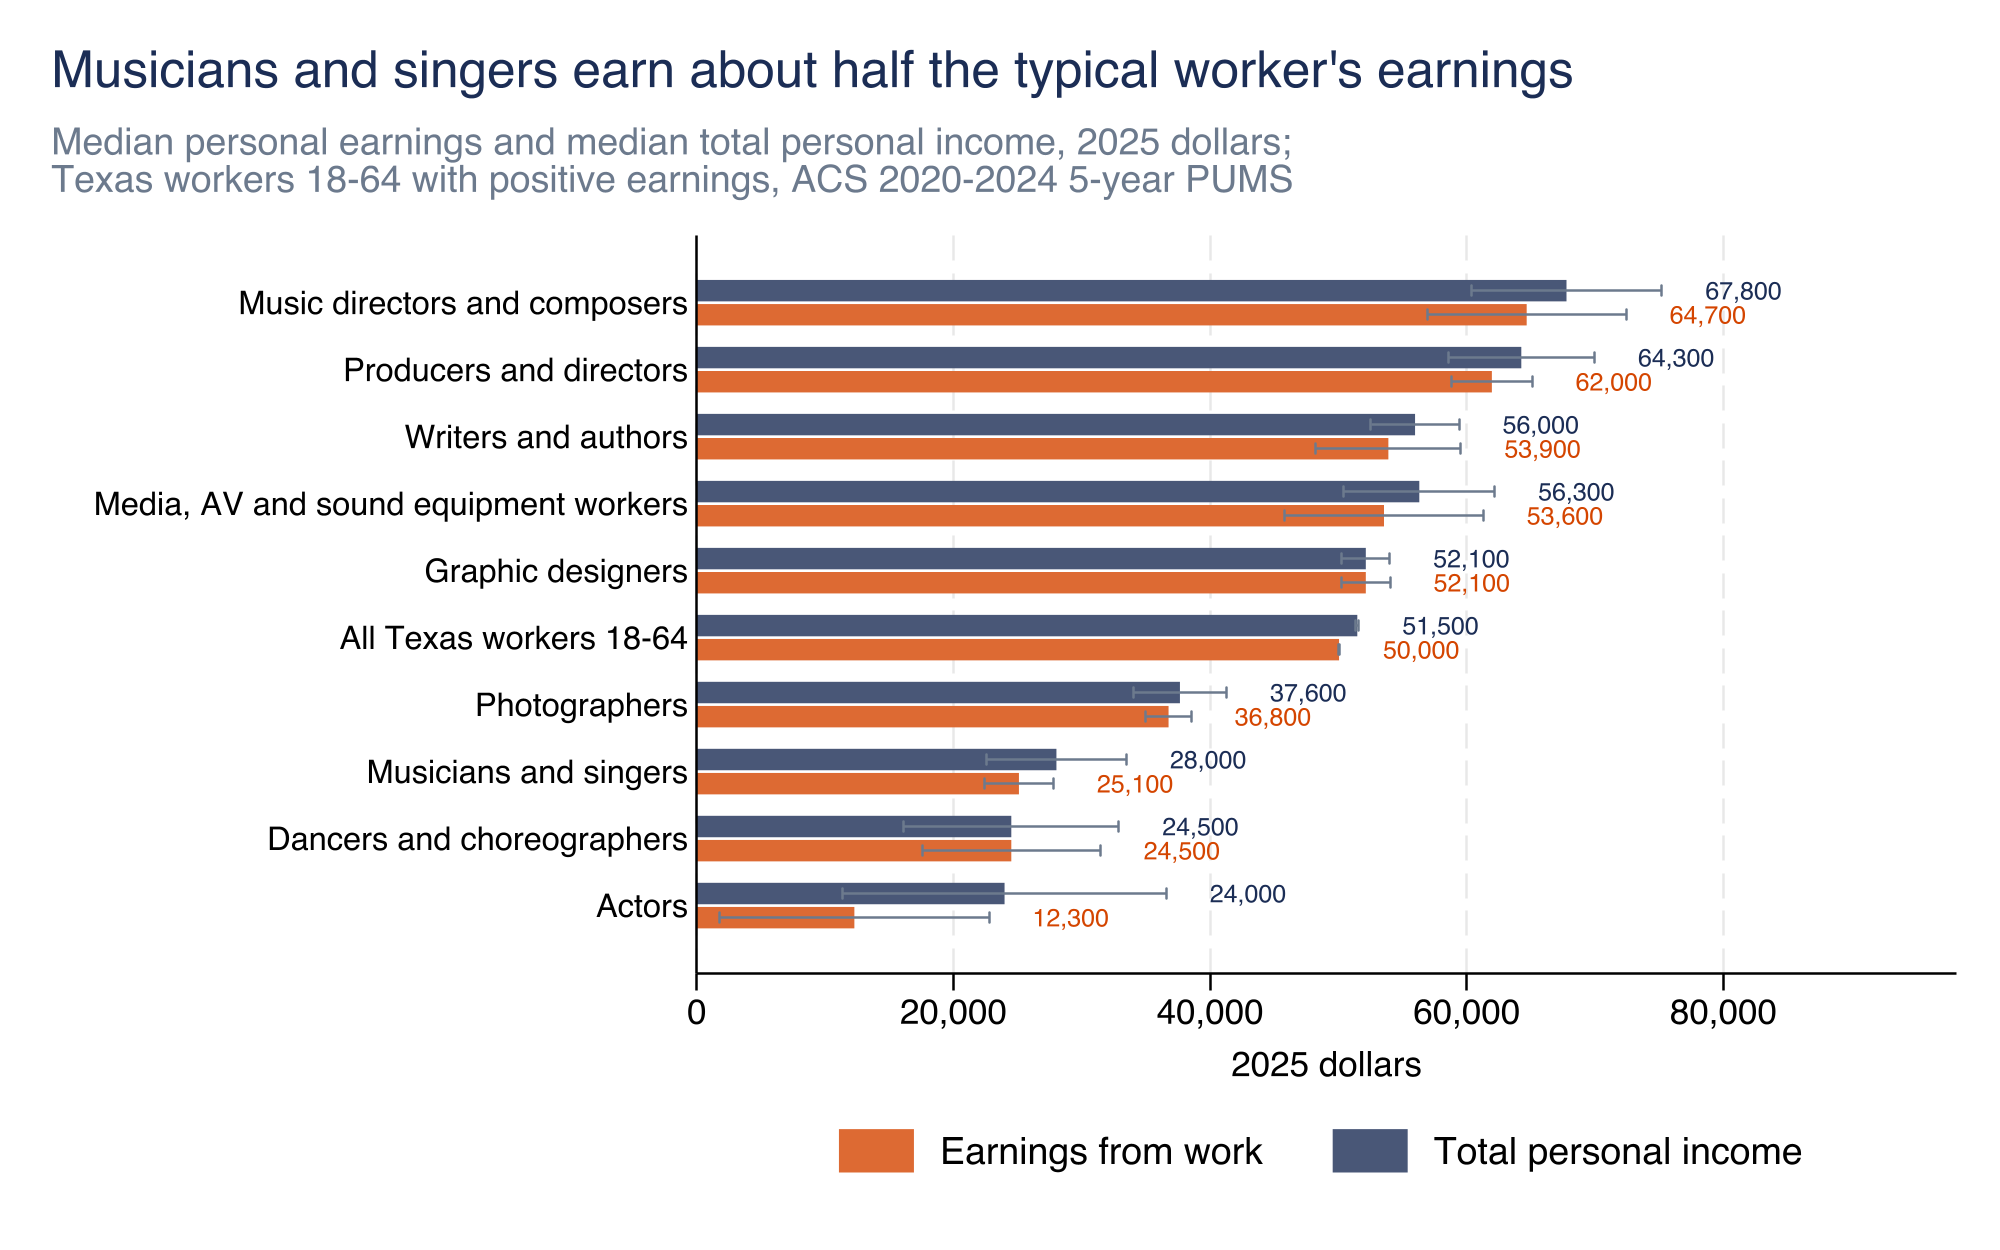
\includegraphics[width=\textwidth]{fig02_earnings_gap.png}
\caption{Median personal earnings from work and median total personal income by
occupation, Texas workers aged 18 to 64 with positive earnings, 2025 dollars.
Source: American Community Survey 2020--2024 five-year public use microdata,
person-weighted; whiskers are 90 percent margins of error from the 80 replicate
weights. How to read it: the orange bar is what the work pays and the navy bar
is total personal income from all sources, so the gap between them is income
from somewhere other than the person's own work. Caveats:
the survey records one occupation per person, so a musician who reports a day
job as their main work is counted in that occupation instead; the combined
media, audio-visual and sound-equipment category is a single Census code, not
sound engineers alone.}
\label{fig:earningsgap}
\end{figure}

Figure~\ref{fig:earningsgap} covers Texas, and what matters in it is less the
ranking than the distance between each occupation's two bars. Actors show the
widest pair, with total personal income roughly twice their earnings from
work; musicians show a smaller but visible pair, and all Texas workers show
almost none. The Austin cell shows the same pattern. Austin musicians report
median total personal income of \NPumsAustinMusMedpincpPos\ against
\NPumsAustinMusMedpernpPos\ in earnings from work. For all Austin workers the
same two figures are \NPumsAustinAllworkMedpincpPos\ and
\NPumsAustinAllworkMedpernpPos, a difference of a few hundred dollars.
The distance between two separately estimated medians is not any one person's
non-work income, but it does say that Austin musicians as a group draw on
income beyond their own work. The survey records income by source in seven
separate fields (wages and salary, self-employment, interest and dividends,
retirement, Social Security, Supplemental Security Income, and public
assistance), and decomposing the gap into those fields would be a direct
extension of the work here.

Hours worked do not account for the low earnings either. The median Austin
musician reports a usual week of \NPumsAustinMusMedwkhp\ hours (the survey
variable WKHP) and \NPumsAustinMusMedwkwn\ weeks worked in the past year
(WKWN), matching \NPumsAustinAllworkMedwkhp\ hours and
\NPumsAustinAllworkMedwkwn\ weeks for the median Austin worker. Both medians
come from the same 77-record Austin cell and both equal the modal answers,
so they say little about the tails: statewide, where the sample is larger,
the median musician's usual week is \NPumsTxMusMedwkhp\ hours against
\NPumsTxAllworkMedwkhp\ for all Texas workers. Firmer evidence comes from
the regression below, which holds hours and weeks fixed and still leaves a
difference.

To probe whether the raw gap comes from age, education, hours or geography
rather than from something specific to music, we estimate a weighted least
squares regression of log personal earnings on an indicator for music
occupations, with controls for age, sex, education, usual hours and weeks
worked, and an indicator for each metro area.\footnote{The fitted equation is
\[
\ln y_i = \alpha + \beta\,\mathrm{music}_i
  + \gamma_1 \mathrm{age}_i + \gamma_2 \mathrm{age}_i^{2}
  + \gamma_3 \mathrm{female}_i
  + \sum_{k=2}^{5}\delta_k\,\mathrm{educ}_{ki}
  + \gamma_4 \mathrm{hours}_i + \gamma_5 \mathrm{weeks}_i
  + \sum_{m}\lambda_m\,\mathrm{metro}_{mi} + \varepsilon_i .
\]
The dependent variable \(y_i\) is person \(i\)'s personal earnings from work
in 2025 dollars (the ACS PERNP field, deflated as described above).
\(\mathrm{music}_i\) is one when the person's occupation is musician, singer,
music director or composer (OCCP 2751 or 2752) and zero otherwise;
\(\mathrm{age}_i\) is AGEP, age in years; \(\mathrm{female}_i\) is one for
women (SEX = 2); the \(\mathrm{educ}_{ki}\) are indicators for four
educational-attainment bands drawn from SCHL, measured against a base of
less than high school (band 2 is high-school diploma or GED, band 3 is some
college, band 4 is bachelor's degree, band 5 is graduate or professional
degree); \(\mathrm{hours}_i\) is WKHP (usual hours worked per week);
\(\mathrm{weeks}_i\) is WKWN (weeks worked in the past twelve months); and
the \(\mathrm{metro}_{mi}\) are Metropolitan Statistical Area indicators
with the Austin-Round Rock-San Marcos MSA as the omitted reference, so each
reported metro coefficient is a difference from Austin and the balance of
the state enters as its own estimated term rather than as the base.
\(\varepsilon_i\) is the residual. Estimation is by weighted least squares
with the person weight PWGTP over the \NPumsRegN\ employed Texans aged 18 to
64 with positive earnings, and the standard error comes from the same 80
replicate weights used for the medians, the Census Bureau's own
successive-difference method, rather than from an assumption that records
are independent. Because the dependent variable is in logs, a coefficient
converts to a percentage difference as \(100\,(e^{\hat\beta} - 1)\), and the
same transformation applied to \(\hat\beta \pm 1.96\,\mathrm{se}(\hat\beta)\)
gives the 95 percent interval. The music coefficient
\NPumsRegMusicCoef\ with standard error \NPumsRegMusicSe\ puts the 95 percent
interval at \(-32.7\) to \(-16.8\) percent. Two things change at once between
this estimate and the Austin medians above: the population is every employed
Texan aged 18 to 64 with positive earnings rather than the Austin metro cell,
and the occupation is musicians, singers, music directors and composers (OCCP
2751 and 2752) rather than musicians and singers alone (OCCP 2752). This is a
descriptive conditional difference, not a causal estimate of what choosing
music does to earnings: people who choose music differ from people who do
not in ways the survey does not record, including talent, family resources
and preference for the work itself. The full three-column table (metro fixed
effects only, plus demographics, plus hours and weeks) is at
\texttt{03\_analysis/out/tables/table\_earnings\_regression.csv}, and the
figures reported in this paragraph come from column (3).}
Among employed Texans aged 18 to 64 with positive earnings from work,
adjusting for age, sex, education, usual hours, weeks worked and metro area,
music occupations show a \NPumsRegMusicPctgap\ earnings difference, against a
raw Austin shortfall of about half. Part of the raw gap therefore tracks
those characteristics and part does not.

\subsection{Most of this workforce works for itself}

\begin{figure}[htbp]
\centering
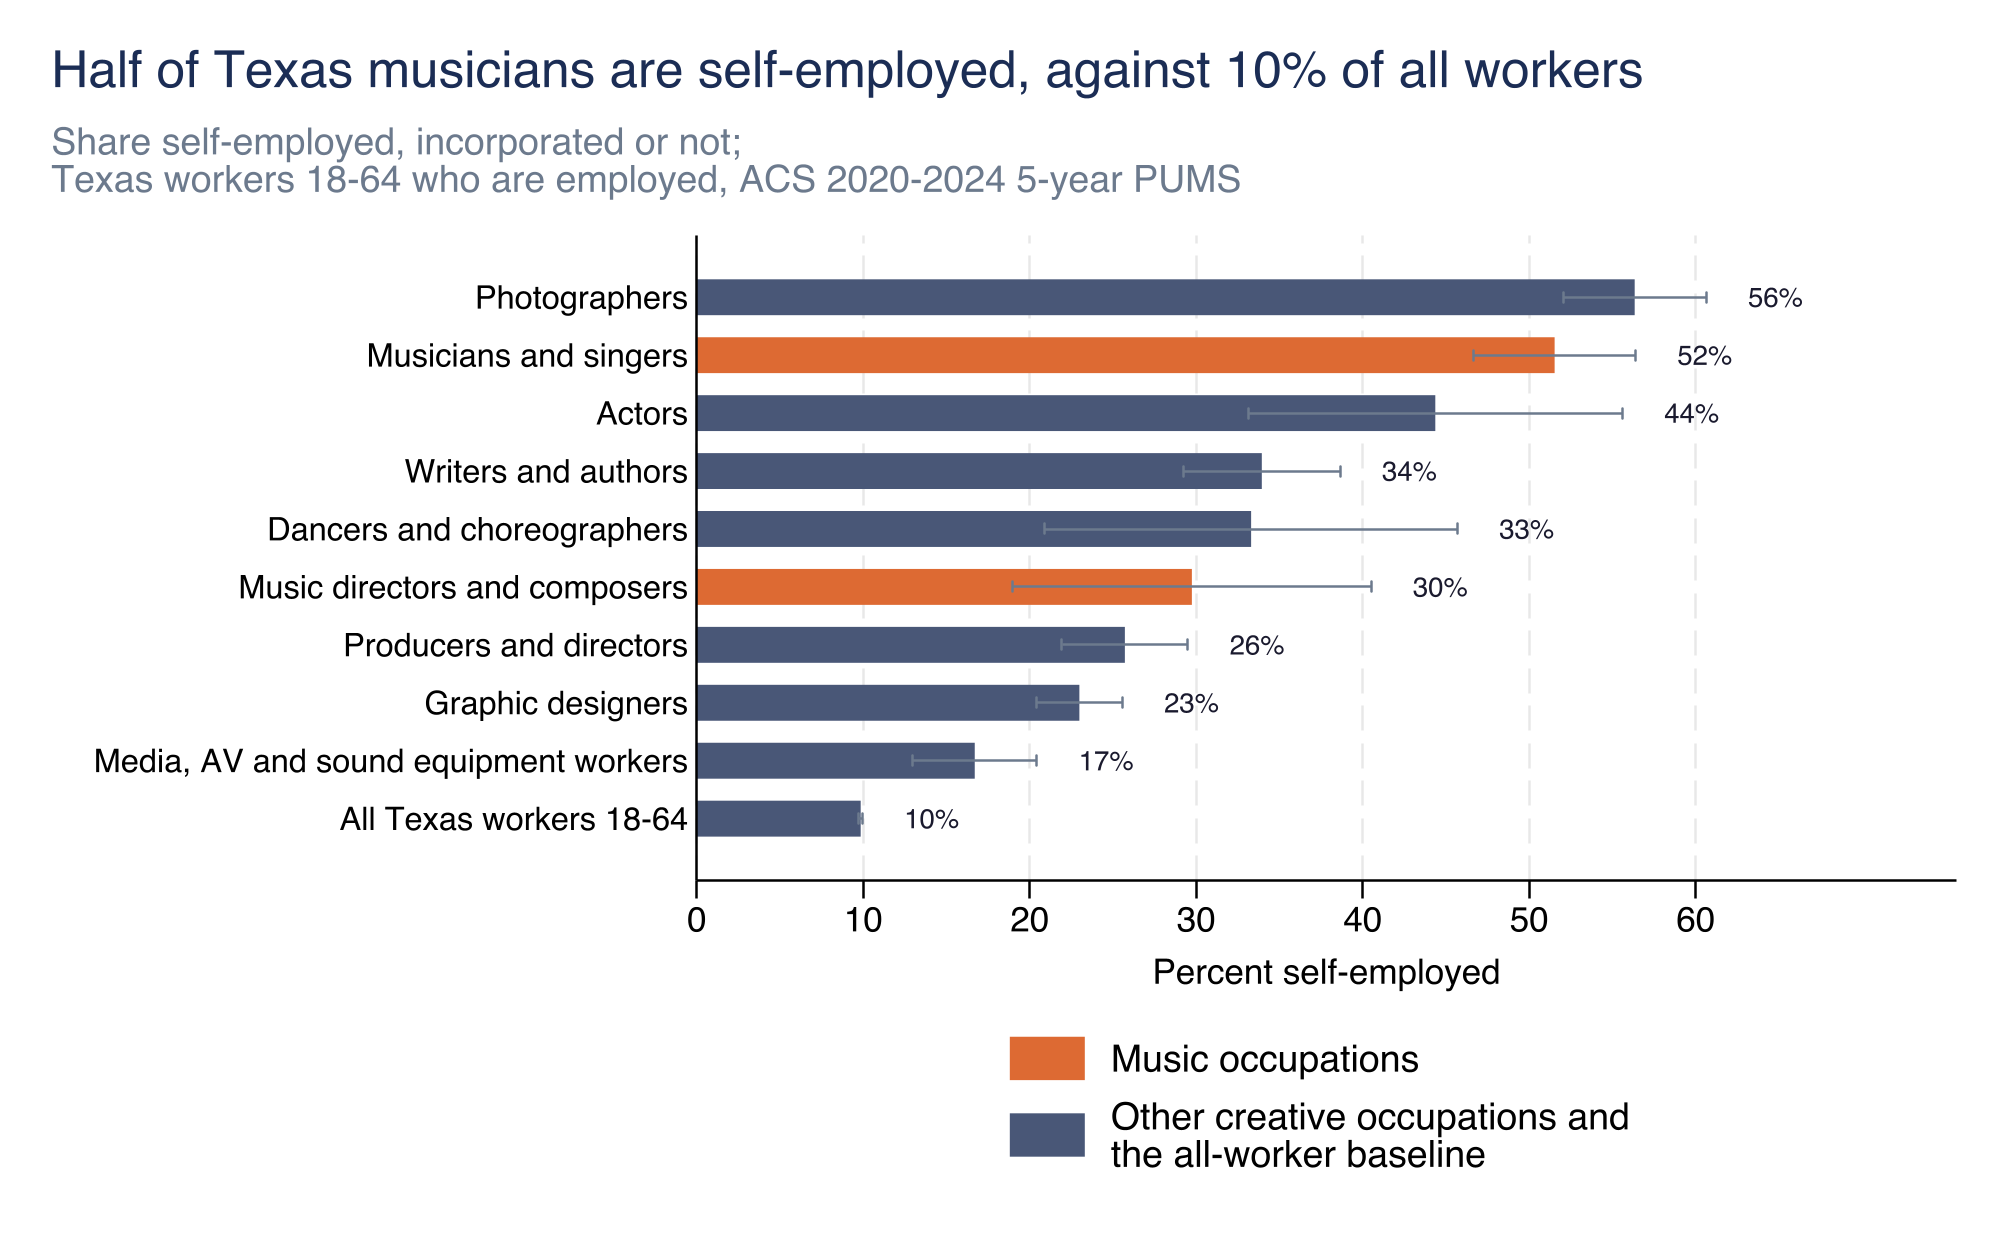
\includegraphics[width=0.86\textwidth]{fig03_selfemp_share.png}
\caption{Share of workers who are self-employed, incorporated or not, by
occupation. Source: American Community Survey 2020--2024 five-year microdata,
employed Texans aged 18 to 64; whiskers are 90 percent margins of error. How to
read it: each bar is the share of workers in that occupation whose main job is
their own business rather than someone else's payroll. Caveat: the survey
records class of worker for the main job only, so a musician who also holds a
payroll day job is counted under the day job.}
\label{fig:selfemp}
\end{figure}

\NPumsAustinMusSelfemp\ (\NPumsAustinMusSelfempMoe) of Austin musicians work
for themselves, against \NPumsAustinAllworkSelfemp\
(\NPumsAustinAllworkSelfempMoe) of all Austin workers, which makes an Austin
musician about seven times as likely to be self-employed as the typical Austin
worker.\footnote{Universe: employed adults aged 18 to 64 in the
Austin-Round Rock-San Marcos MSA, ACS 2020--2024 five-year Texas PUMS. The
numerator on both sides is class-of-worker categories 6 (self-employed,
unincorporated) and 7 (self-employed, incorporated) from the survey's COW
field; the denominator is the employed base on that geography. The musician
share comes from \NPumsAustinMusNEmp\ unweighted person records, so we do not
break it down by demographic subgroup.} Statewide the musician rate is lower,
\NPumsTxMusSelfemp\ (\NPumsTxMusSelfempMoe) against \NPumsTxAllworkSelfemp\
for all Texas workers, so the Austin estimate is well above the state
estimate on a cell of only \NPumsAustinMusNEmp\ records and should be read
with that in mind.

Self-employment at that rate accounts for much of the distance between the
payroll count and the survey count, though not all of it. Applying the Austin
self-employment share to the \NPumsAustinMusWtdPos\ musicians the survey
estimates leaves roughly 600 on someone's payroll, against the
\NEmpPayrollMusiciansAustinLast\ jobs the federal wage survey recorded in the
Austin metro in 2025.\footnote{The federal wage survey here is the Bureau of
Labor Statistics Occupational Employment and Wage Statistics (OEWS) program,
a semi-annual establishment survey administered by BLS and the state
workforce agencies. Program documentation:
\url{https://www.bls.gov/oes/oes_ques.htm}. OEWS reports the wage of every
worker on a sampled establishment's payroll and reports nothing for the
self-employed, who fall outside its sampling frame; that is the arithmetic
reason a survey which counts self-employment income and a payroll survey
which does not disagree so widely on the same occupation and the same metro.
Section~\ref{sec:payroll} takes up the payroll count separately.} It also
explains why a payroll-based wage series can look healthy while a survey
which counts self-employment income does not.

\subsection{The distribution matters more than the median}

\begin{figure}[htbp]
\centering
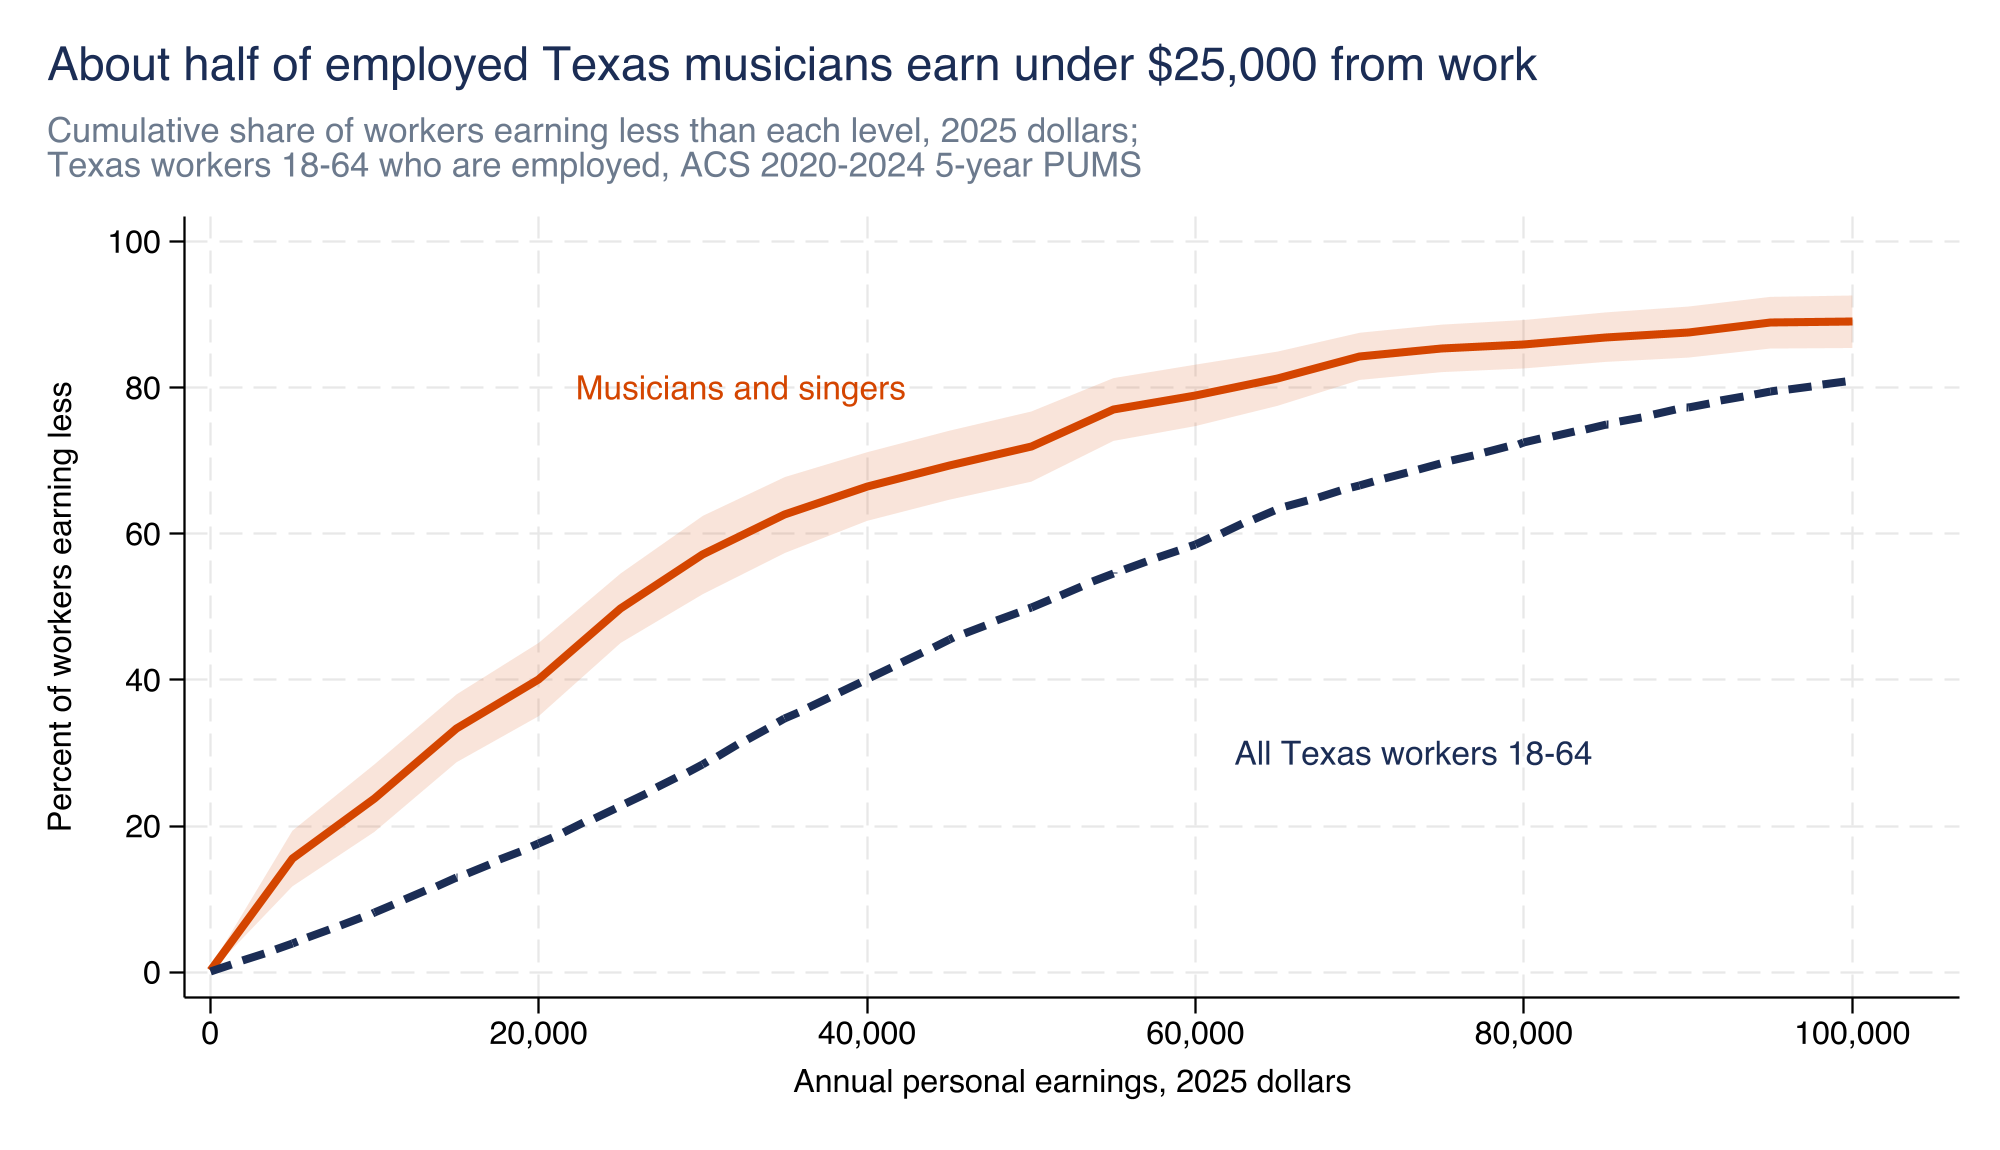
\includegraphics[width=0.86\textwidth]{fig04_earnings_distribution.png}
\caption{Cumulative share of workers earning below each level, musicians against
all workers, Texas, 2025 dollars. Source: American Community Survey 2020--2024
five-year microdata, employed adults 18 to 64 with positive earnings. How to
read it: the height of a line at a given earnings level is the share of that
group earning less than that amount, so a line sitting higher and further left
means more of the group earns little. Caveat: earnings here come from all work,
not from music alone, so a musician with a day job appears at the combined
figure.}
\label{fig:earningsdist}
\end{figure}

The spread below the median is wide. Figure~\ref{fig:earningsdist} plots
Texas, where the sample is large enough to draw a smooth curve; the shares
below are for the Austin cell, which comes from 77 records and so has
margins of error several times wider.
\NPumsAustinMusLtOneZerok\ (\NPumsAustinMusLtOneZerokMoe) of employed Austin
musicians aged 18 to 64 earn under \$10,000 from work, against
\NPumsAustinAllworkLtOneZerok\ (\NPumsAustinAllworkLtOneZerokMoe) of all
employed Austin workers on the same base;
\NPumsAustinMusLtTwoFivek\ (\NPumsAustinMusLtTwoFivekMoe) earn under
\$25,000 against \NPumsAustinAllworkLtTwoFivek; and
\NPumsAustinMusLtFiveZerok\ (\NPumsAustinMusLtFiveZerokMoe) earn under
\$50,000 against \NPumsAustinAllworkLtFiveZerok. Measured against the
\$10,000 line the 2014 Austin Music Census drew for 2013 music income,
restated to today's prices,\footnote{The 2013 threshold is the \$10,000 line the
2014 Austin Music Census applied to its respondents' 2013 pre-tax music
income. Titan Music Group, LLC, for the City of Austin Economic Development
Department, Music and Entertainment Division, \textit{The Austin Music
Census: A Data-Driven Assessment of Austin's Commercial Music Economy}
(fielded late 2014; published June 1, 2015; income data are pre-tax calendar
2013), \url{https://austin.widen.net/content/om7zqn1qbx/pdf/Austin_Music_Census_Interactive_PDF_53115.pdf}.
That census was a self-selected online convenience sample of 3,968
respondents drawn from the Austin music community; its published shares
describe the people who answered, and no probability-sample margin of error
attaches to them. Its microdata were never publicly released.}
\NPumsAustinMusLtmusiccensus\ (\NPumsAustinMusLtmusiccensusMoe) of Austin
musicians fall below the line that census drew, against
\NPumsAustinAllworkLtmusiccensus\ of the wider Austin workforce. That share
is not comparable with the 2014 census's own 68.4 percent: the 2014 census
measured music income only, among self-selected respondents, while the ACS
figure measures earnings from all work on a probability sample eight years
later.\footnote{Each share is the weighted proportion defined above,
\(\hat p = \sum_i w_i\,\mathbf{1}(y_i < \bar y)\big/\sum_i w_i\), where
\(\bar y\) is the threshold and \(y_i\) is personal earnings in 2025 dollars.
These four shares use the employed base (employed Austin musicians aged 18
to 64), rather than the positive-earnings base used for the medians above:
people reporting zero or negative earnings from work stay in the
denominator, because dropping them would remove the worst-off cases from a
statistic whose subject is how many people fall below a low threshold. The
2013 threshold is carried forward as
\(\$10{,}000 \times d_{2013}\), where \(d_{2013} = C_{2025}/C_{2013}\) is the
ratio of CPI-U annual averages, equal to
\NPumsDeflTwoZeroOneThreeToTwoZeroTwoFive, which puts the line at
\NPumsMusiccensusTenkTwoZeroTwoFiveusd\ in today's prices.}

\subsection{Nothing suggests Austin pays musicians better than other Texas metros}

Austin's median-musician earnings are lower than the medians in Dallas-Fort
Worth and Houston, but only by amounts small enough that the sampling error
in each metro cell easily covers the difference. These three metro figures
pool musicians, singers, music directors and composers (OCCP 2751 and 2752),
a wider grouping than the musicians-and-singers headline above, which is
what makes the metro cells large enough to publish.\footnote{The pooled
sample sizes are: Austin \NPumsMetroAustinMusicN\ unweighted records
representing \NPumsMetroAustinMusicWtd\ people; Dallas-Fort Worth 191 records
representing 4,505 people; Houston 117 records representing 3,453 people.
Each cell is drawn from the ACS 2020--2024 five-year Texas PUMS, employed
adults aged 18 to 64 with positive earnings, and each metro is its full
five- or ten-county MSA as defined by OMB's 2023 core-based statistical area
delineation. Musicians and singers alone (OCCP 2752) yield 33 Dallas records
and 26 Houston records, both under the 50-record suppression threshold this
study uses.} Median personal earnings from work in these pooled music
occupations are \NPumsMetroAustinMusicMedpernp\
(\NPumsMetroAustinMusicMedpernpMoe) in Austin,
\NPumsMetroDfwMusicMedpernp\ (\NPumsMetroDfwMusicMedpernpMoe) in Dallas-Fort
Worth and \NPumsMetroHoustonMusicMedpernp\
(\NPumsMetroHoustonMusicMedpernpMoe) in Houston. Austin has the lowest point
estimate of the three, and every margin is wide, so neither pairwise gap is
statistically firm.\footnote{Austin against Houston is a difference of about
\$12,500 against a combined 90 percent margin of roughly \$18,600; Austin
against Dallas-Fort Worth is about \$5,300 against roughly \$17,500. The
margin on a difference between two metro medians is
\(\mathrm{MOE}_{A-B} = \sqrt{\mathrm{MOE}_A^{2} + \mathrm{MOE}_B^{2}}\),
where \(\mathrm{MOE}_A\) and \(\mathrm{MOE}_B\) are the two 90 percent
margins computed from the replicate weights. The square-root form assumes
the two metro subsamples are independent, which is the usual assumption for
non-overlapping geographies in this file, and it is narrower than adding the
two margins; a gap smaller than that combined margin is one the data cannot
distinguish from zero. Nothing in these three medians supports an assumption
that the Live Music Capital pays its musicians better than the rest of the
state, and nothing in them establishes that it pays them worse.}

\subsection{Austin musicians hold health coverage at roughly the workforce rate}

Health coverage among Austin musicians is \NPumsAustinMusHicov\
(\NPumsAustinMusHicovMoe) against \NPumsAustinAllworkHicov\
(\NPumsAustinAllworkHicovMoe) for all Austin workers, a difference well
inside the musician margin, so the two rates are indistinguishable at the
sample sizes at hand.\footnote{Both shares use the survey's HICOV variable,
which is one when the respondent reports any health insurance coverage
(private, public or both) at the time of the interview, and zero otherwise.
Universe: employed adults aged 18 to 64 in the Austin-Round Rock-San Marcos
MSA, ACS 2020--2024 five-year Texas PUMS; the musician side comes from 77
unweighted records (OCCP 2752), the all-workers side from 48,643. Private and
public coverage are recorded separately (PRIVCOV and PUBCOV) and overlap for
respondents who hold both, so those two shares do not sum to HICOV.}
Private coverage runs the other way: \NPumsAustinMusPrivcov\
(\NPumsAustinMusPrivcovMoe) of Austin musicians hold private insurance
against \NPumsAustinAllworkPrivcov\ for the wider workforce, so the
any-coverage parity rests on public coverage, and possibly on Austin's
music-specific nonprofit health infrastructure, rather than on
employer-sponsored plans.

The 2022 Greater Austin Music Census reports that 84 percent of its
respondents held health coverage in 2022, up from 79 percent in the 2014
census, and its authors attribute that five-point rise to the Health
Alliance for Austin Musicians.\footnote{Sound Music Cities and City of
Austin Music \& Entertainment Division, \emph{2022 Greater Austin Music
Census}, Data Appendix pp.\ 72--73 and Summary Report p.\ 10. Both
comparison figures are self-selected respondent shares rather than
population estimates, and the two censuses are not comparable samples, so
this is a change in reported coverage among the people who answered rather
than a measured change in the workforce as a whole.} The Health Alliance
for Austin Musicians, HAAM, is a 501(c)(3) launched in 2005 that enrols
low-income working Austin musicians (a 400 percent-of-federal-poverty-line
eligibility ceiling) in a coordinated network of primary care, dental,
vision, mental-health and hearing services at subsidised
fees.\footnote{Health Alliance for Austin Musicians, \emph{Annual Impact
Report}, 2005 through 2025 series at
\url{https://www.myhaam.org/annual-reports}. Retrieved 1 August 2026.
Membership rose from 450 in 2005 to 3{,}136 in 2022 and 3{,}149 in 2023;
cumulative healthcare value delivered rose from an initial-year figure of
\$115{,}000 in 2005 to \$46 million (2015), \$73.7 million (2019), \$123
million (2022) and \$215 million (2025), figures drawn from HAAM's own
annual reports. HAAM publishes a member-income share-below-threshold rather
than a member median, so the report does not treat its threshold statistics
as earnings measurements of the wider Austin musician workforce.} SIMS
Foundation, founded in 1995, delivers mental-health and substance-use care
to Austin musicians and their families on a similar
reduced-fee model.\footnote{SIMS Foundation, at
\url{https://simsfoundation.org/about/}, retrieved 1 August 2026.} The ACS
does not identify HAAM or SIMS enrolees, so the coverage rate here is not
causally attributable to either organisation, but the parity is consistent
with what the census reports.

\subsection{Musician households in Texas pay a higher median rent when they rent}

Among Texas households with a working adult, musician households and other
working households rent at close to the same rate: about 41 percent of
musician households are renters, against 39 percent of working households as
a whole.\footnote{Renter shares are weighted-household ratios computed from
the ACS 2020--2024 five-year Texas PUMS housing extract, using weighted
renter and owner household counts, so the two shares are computed on
comparable denominators; the small difference is well inside the musician
margin. Age composition is also similar: the median age of the householder
is close in the two groups, so tenure differences do not reduce to a
younger-therefore-not-yet-owning composition effect at the level the
household file can measure. The Austin metro sub-cell is too small to
publish tenure shares for.} \emph{Among renter households}, musician
households pay a higher median gross rent than working households as a
group.\footnote{The rent statistics come from the ACS housing extract for
Texas (2020--2024 five-year PUMS), a separate file with its own household
weight WGTP and its own 80 replicate weights (WGTP1--WGTP80), used in the
same successive-difference formula as above. Rent is put on 2025 dollars
by ADJHSG (which restates the five survey years on a 2024 basis) and the
same CPI-U 2024-to-2025 factor. Universe: Texas households with at least
one employed resident aged 18 to 64. A household counts as a musician
household when at least one of those employed residents reports OCCP 2752
(Musicians and Singers) as their current or most recent occupation; the
comparison group is every Texas household with at least one employed
resident, so the two groups nest rather than partition, and the comparison
is musician households against all working households, not against a
mutually exclusive remainder. The two sample sizes are 160 unweighted
musician-renter households (representing 4,552 weighted households) and
101,799 unweighted worker-renter households (representing 3.14 million).
Both figures are Texas households rather than Austin ones, because the
Austin-only musician cell is too small in the household file to publish.}
The median monthly gross rent is \NPumsHhMusMedrent\ for musician renter
households against \NPumsHhWorkerMedrent\ for renting Texas worker
households. The rent level is higher, but the burden is not:
\NPumsHhMusRentThreeZero\ (\NPumsHhMusRentThreeZeroMoe) of musician renter
households pay more than 30 percent of household income in
rent\footnote{The rent-burden variable is GRPIP, gross rent as a percentage
of household income, computed by the Bureau from monthly gross rent (GRNTP,
which is contract rent plus tenant-paid utilities) and household income
(HINCP). GRPIP is a ratio of two same-year quantities, so no inflation
adjustment applies; it is top-coded at 101, a category the Bureau also uses
for households reporting zero or negative income. The 30 percent line is the
standard federal cost-burden threshold used by HUD.} against
\NPumsHhWorkerRentThreeZero\ (\NPumsHhWorkerRentThreeZeroMoe) of working
renter households as a whole, a gap well inside the musician margin. Read
together: a musician-renter household in Texas signs a lease on a more
expensive unit than the average working-renter household does, but pays
roughly the same share of household income for it, likely because a second
earner or non-earnings income (a topic Section~\ref{sec:costs} takes up)
makes the rent-to-income ratio hold even as the rent bill runs higher. What
the household file cannot say is why the rent bill runs higher, since the ACS
does not record which parts of the metro a household lives in or which
features of the unit drive its rent.

% Section 3: the cost side. Two housing figures in this section look
% contradictory unless the text says which measure it is using and where each
% measure comes from, so the reconciliation is explicit and every rent source is
% named with its universe and vintage at first mention.
\section{Austin is an average-cost city with expensive housing}
\label{sec:costs}

What Austin musicians earn matters only against what living in Austin costs.
Austin is often described in local reporting and in national coverage as an
expensive city across the board, from groceries to rent to services, but the
federal price record narrows that picture: Austin runs close to the national
average on most goods and services and above the national average only in
housing.\footnote{Framings that treat Austin as broadly expensive appear in
national coverage such as U.S.\ News \& World Report's cost-of-living
rankings and in Austin American-Statesman and Axios Austin coverage of
city-affordability trends; this study does not enumerate that literature
here, and the BEA Regional Price Parities cited in the next sentence are
the federal counterpoint.} The Bureau of
Economic Analysis publishes an annual price comparison across metro areas
called the Regional Price Parities (RPP), which measures the price of a common
basket of goods and services in each metro against a national average set to
100 and reports it separately for four component baskets, one of which is
housing services.\footnote{The BEA program is the \textit{Regional Price
Parities and Implicit Regional Price Deflators by MSA}, currently released in
its 2024 vintage covering years 2008 through 2024, and available from the
Bureau of Economic Analysis at
\url{https://apps.bea.gov/regional/zip/MARPP.zip}. The universe is the
population of each metropolitan statistical area, and the basket weights come
from the Consumer Expenditure Survey. Each metro's all-items index is a
weighted average of the four component indexes, so the housing component and
the all-items index sit on the same national base of 100 and their difference
in the same metro is in index points rather than percent. BEA publishes no
sampling error for these estimates because the underlying price series are
themselves published indexes rather than sample statistics.} On the 2024 BEA
figures, Austin's all-items index is \NColRppAllitemsAustin\ against the
national average of 100, marginally below the national average across all
goods and services. Austin's housing services index is
\NColRppHousingAustin, so housing costs in Austin run
\NColRppGapAustin\ higher than everything else does in the same city. That
place gap is the widest of the five metros compared here, ahead of
Dallas \NColRppGapDallas, Nashville \NColRppGapNashville, Houston
\NColRppGapHouston, and San Antonio essentially none at
\NColRppGapSanantonio.\footnote{The gap reported for each metro is
\(g_m = \mathrm{RPP}^{\mathrm{hous}}_m - \mathrm{RPP}^{\mathrm{all}}_m\), the
difference in index points between that metro's housing parity and its own
all-items parity, so it measures how much more expensive housing is than
everything else in the same place rather than how expensive that place is
against another one. Because both terms are indexed to the same national base
of 100, the difference is in index points and is not a percentage. Austin's
housing parity peaked at \NColRppAustinHousingPeak, a peak year the two
independent housing series in Figure~\ref{fig:metrorent} corroborate.}

The national price record shows the same relative movement over time, in a
different measure. The Bureau of Labor Statistics tracks the price of a fixed
consumer basket each month in its Consumer Price Index for All Urban Consumers
(CPI-U), for a universe of the urban population of the United States, and
reports the all-items index and its components on a common
base.\footnote{The series are the CPI-U All items (series identifier
CUUR0000SA0) and the CPI-U Housing component, U.S.\ city average, monthly, and
this study rebases each to its 2005 annual average and takes the 2025 annual
average of each rebased series. Program documentation is available from BLS at
\url{https://www.bls.gov/cpi/}. BLS publishes no Austin-area CPI at all, so
every real-dollar figure in this report deflates by the national U.S.\ city
average CPI-U, and given the RPP evidence above that Austin housing runs above
the national norm, this national deflator most likely understates the true
Austin price rise. The 2025 annual average of the housing component uses an
interpolated October, because the federal funding lapse suspended BLS price
collection that month.} Rebased so that each series equals 100 in 2005, the
housing component reaches \NColCpiHousingIndexTwoZeroTwoFive\ by 2025 against
\NColCpiAllitemsIndexTwoZeroTwoFive\ for all items, so national housing prices
have risen \NColCpiHousingGapTwoZeroTwoFive\ faster than the broad basket since
2005.\footnote{Rebasing on 2005 puts \(I^{s}_{t} = 100 \times C^{s}_{t} /
C^{s}_{2005}\), where \(C^{s}_{t}\) is the annual average of the CPI-U for
series \(s\), either all items or the housing component, in year \(t\).
Putting both series on the same base year is what makes them comparable, and
the gap is the difference of the two rebased levels in 2025,
\(I^{\mathrm{hous}}_{2025} - I^{\mathrm{all}}_{2025}\), again in index points
rather than percent. This national CPI comparison and the BEA metro parity
above answer different questions and are not comparable in level: the
CPI-Housing figure describes the national price rise for housing since 2005,
and the RPP-Housing figure above describes where the Austin metro sits against
the current national average.}

For Austin musicians the cost problem concentrates in housing, the one BEA
category that prices well above the national norm in Austin. The rest of this
section follows housing: what market rents have done since 2015, how many
hours of work a month of rent costs at Austin wages, and why those two figures
appear to disagree.

\subsection{Rents rose sharply, then fell further than in any comparison metro}

\begin{figure}[htbp]
\centering
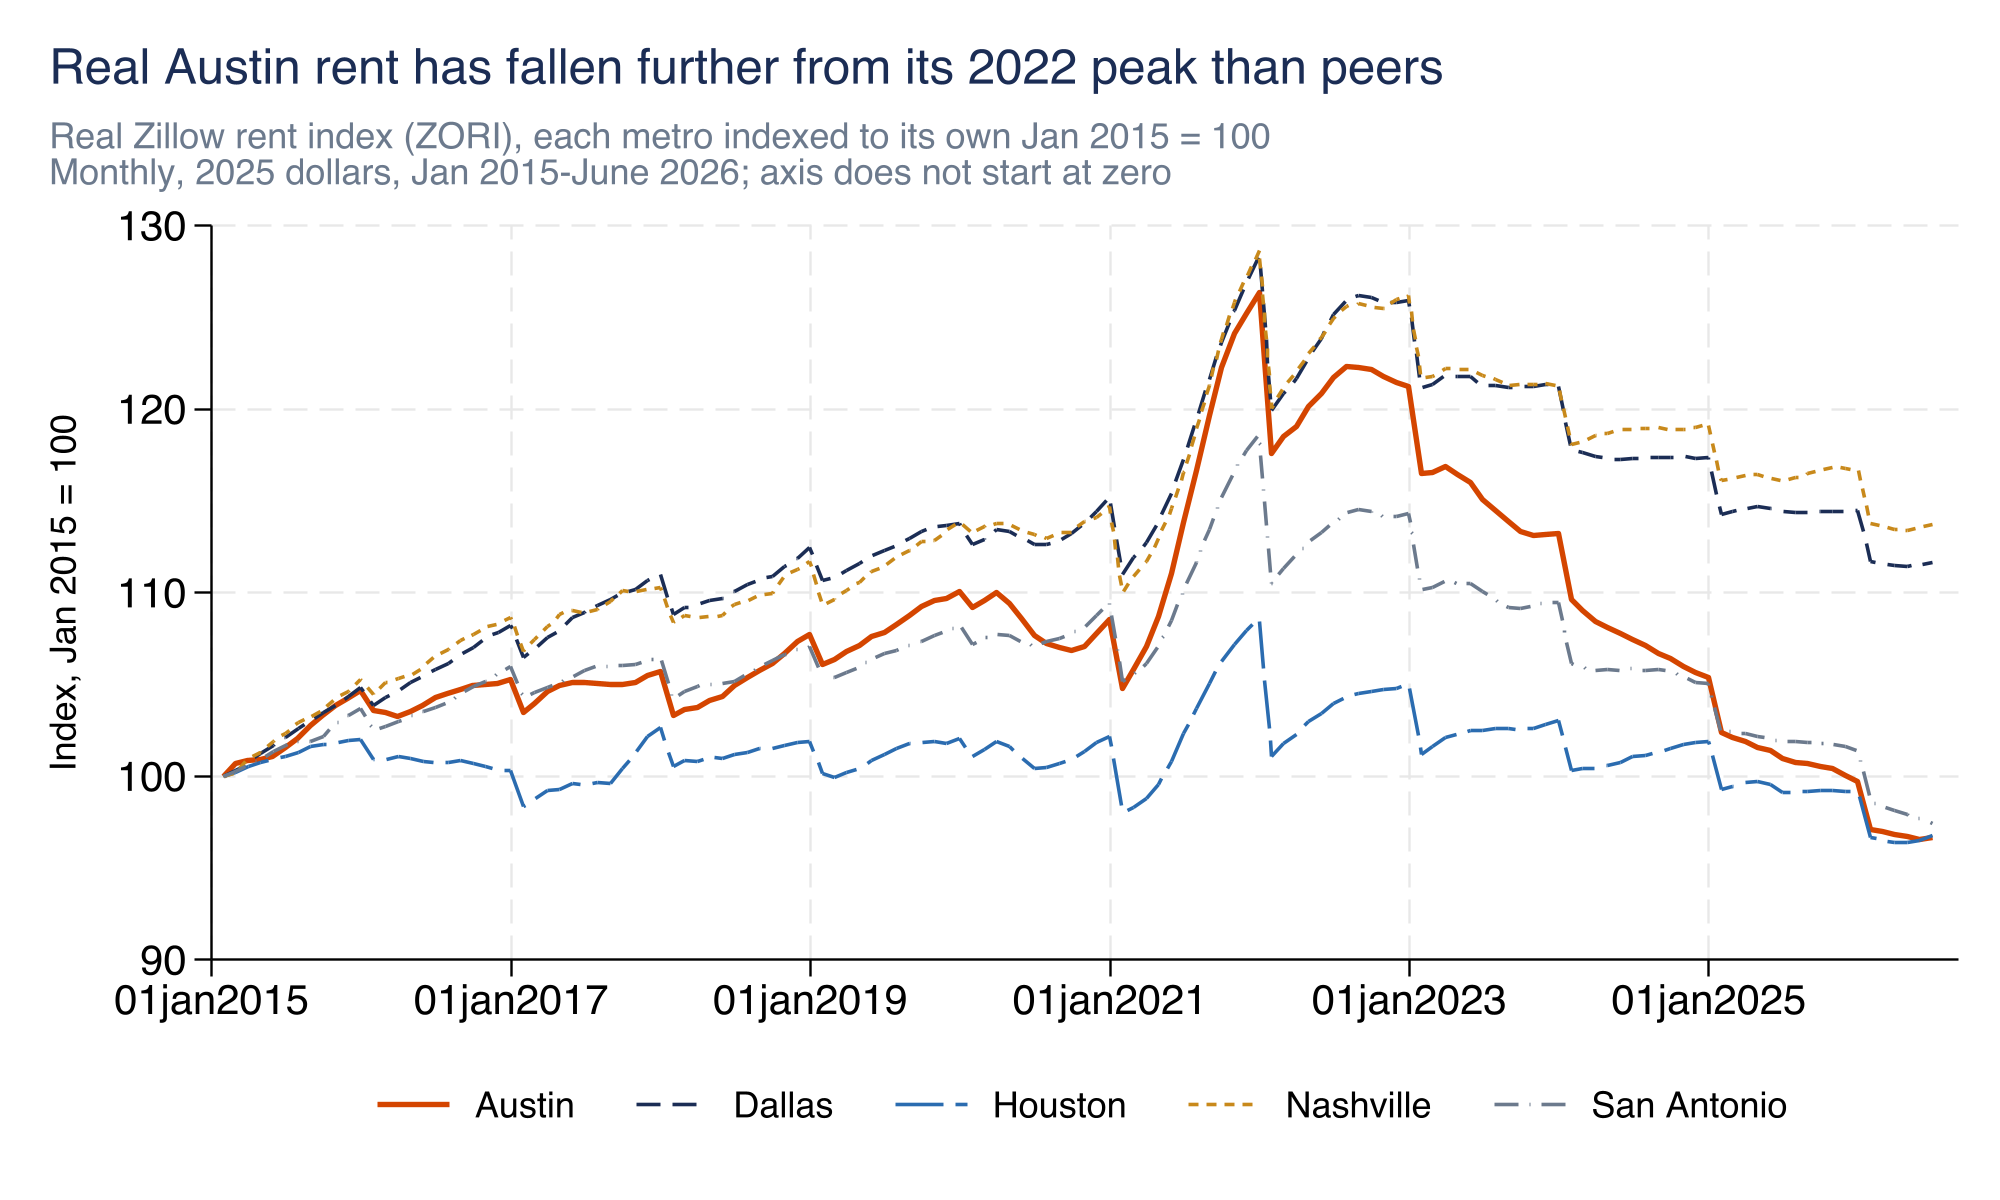
\includegraphics[width=\textwidth]{fig20_metro_rent.png}
\caption{Real market rent indexed to each metro's own January 2015 level, 2025
dollars, through June 2026. Source: Zillow Observed Rent Index (ZORI),
seasonally adjusted, deflated with the national Consumer Price Index for All
Urban Consumers. How to read it: each line shows how far that metro's real
rent has moved from its own 2015 starting point, so the lines compare
trajectories rather than rent levels. Note on timing: Austin's real peak is
December 2021, about a year before the widely quoted nominal peak, because
deflating during the sharp inflation of 2021 to 2023 shifts the turning point
earlier. Both readings are correct and answer different questions. Caveat: the
small step every line takes at each January is the annual deflator changing,
not a change in rents, because a single year-average price index is applied to
twelve months of rent data.}
\label{fig:metrorent}
\end{figure}

Zillow's Observed Rent Index estimates the typical asking rent in each metro
each month by weighting an internal repeat-rent index against local rental
market shares, and it is the closest thing in the public record to a monthly
Austin rent series, because BLS publishes no Austin-area consumer price
index.\footnote{Zillow Group publishes the seasonally adjusted metro-level
ZORI series at \url{https://www.zillow.com/research/data/}, together with a
methodology document. The universe is rental listings on the Zillow platform,
weighted to the U.S.\ Postal Service's count of the rental housing stock in
each geography, so ZORI captures the rent asked on newly available units
rather than the rent paid on all standing leases. It is not a probability
sample of dwellings, and Zillow does not attach a sampling error to it. It
runs monthly at the metro level and picks up cyclical turns faster than the
Census Bureau's American Community Survey median gross rent, which pools five
years of household responses and moves slowly by construction.} On that
series, Austin's real market rent peaked at \NColZoriAustinPeak\ and has
fallen \NColZoriAustinPeaktolatest\ since, the steepest decline among the five
metros in Figure~\ref{fig:metrorent}, with San Antonio the nearest at
\NColZoriSanantonioPeaktolatest\ and Dallas
\NColZoriDallasPeaktolatest\ and Houston
\NColZoriHoustonPeaktolatest.\footnote{The plotted series deflates each metro
first and rebases second. The real level is
\(R^{\mathrm{real}}_{m,t} = R_{m,t} \times d_{y(t)}\), where \(R_{m,t}\) is
the seasonally adjusted ZORI value for metro \(m\) in month \(t\), \(y(t)\)
is the calendar year containing that month, and \(d_y = C_{2025}/C_y\) is
the ratio of national CPI-U annual averages that carries year \(y\) dollars
to 2025 dollars. The plotted line is then
\(I_{m,t} = 100 \times R^{\mathrm{real}}_{m,t} \big/
   R^{\mathrm{real}}_{m,\text{Jan }2015}\),
each metro against its own base month, which removes the level and leaves the
trajectory, so metros at different rent levels can share one axis. The
peak-to-latest change is
\(100\,\bigl(R^{\mathrm{real}}_{m,\text{latest}} \big/
   R^{\mathrm{real}}_{m,\text{peak}} - 1\bigr)\)
on the deflated series. Deflating with an annual CPI-U during the sharp
inflation of 2021 to 2023 is what moves the real peak about a year ahead of
the nominal one: the step in \(d_y\) between 2021 and 2022 outweighs the
further nominal rent increase in that year.} Home values fell further still.
Zillow's Home Value Index (ZHVI), a repeat-sales estimate of the typical
market value of a single-family home in the metro, records an Austin peak of
\NColZhviAustinPeak\ and a real decline of
\NColZhviAustinPeaktolatest\ from it.\footnote{Zillow Group publishes the
metro-level ZHVI (all homes, seasonally adjusted) at the same research portal,
\url{https://www.zillow.com/research/data/}. The universe is the middle tier
of homes valued between the 35th and 65th percentiles in each geography,
estimated monthly from Zillow's proprietary automated valuation model and
transaction records. ZHVI is a market-value estimate rather than a
transaction-price series, so it can move faster than recorded sales prices
where turnover thins, and no sampling error attaches to it.} A report that
showed only the run-up and stopped in 2022 would be describing a market that
no longer exists.

The federal housing-assistance benchmark moved differently. The Department
of Housing and Urban Development publishes an annual Fair Market Rent (FMR)
for each metropolitan area, one figure per bedroom count, and sets it near
the 40th percentile of standard-quality rents in the area, using a rolling
five-year window of American Community Survey responses updated with more
recent private data.\footnote{The all-years FMR history is available from
HUD at \url{https://www.huduser.gov/portal/datasets/FMR/FMR_All_1983_2026.csv}.
The FMR is the reference point for what the federal Housing Choice Voucher
program, and other HUD rental-assistance programs, will pay in each metro
area. It is a benchmark, not an observed rent: HUD constructs it from ACS
five-year survey data on gross rent for standard-quality units and then
trends it forward with more recent private rent indexes. The universe is
recent movers within the metro, so FMR turns later than a market series like
ZORI. Two breaks in the source sit inside this study's window and make the
peak date and the peak-to-latest change approximate: the nominal one-bedroom
Austin rent jumps 18.0 percent between FY2023 and FY2024, the same year the
file's percentile-basis field goes blank, and the FY2026 value is published
for a redefined metro area, Austin-Round Rock-San Marcos rather than
Austin-Round Rock.} HUD's Austin one-bedroom FMR peaked later, at
\NColHudBrOneAustinPeak, and has come down only
\NColHudBrOneAustinPeaktolatest\ since.\footnote{Both housing series in this
subsection use the same deflator and dating rule as the market rent above,
\(F^{\mathrm{real}}_y = F_y \times d_y\) followed by
\(100\,(F^{\mathrm{real}}_{\mathrm{latest}}/F^{\mathrm{real}}_{\mathrm{peak}}
   - 1)\), so both are in constant 2025 dollars. The hours-of-work ratio in
the next subsection uses the same HUD Fair Market Rent in nominal dollars
instead, because there the rent is divided by a same-year wage and deflating
both sides would cancel.} Austin's assistance benchmark turned about two and
a half years after the market series did. That lag matters for any program
priced off the benchmark rather than off the market, and it is the larger
part of the tension between the next two figures. The rest of that tension is
that the payroll musician wage the next figure divides by fell back from an
unusually high 2022 reading in the years HUD's FMR was still rising.

\subsection{The payroll wage understates what rent takes from musicians}

\begin{figure}[htbp]
\centering
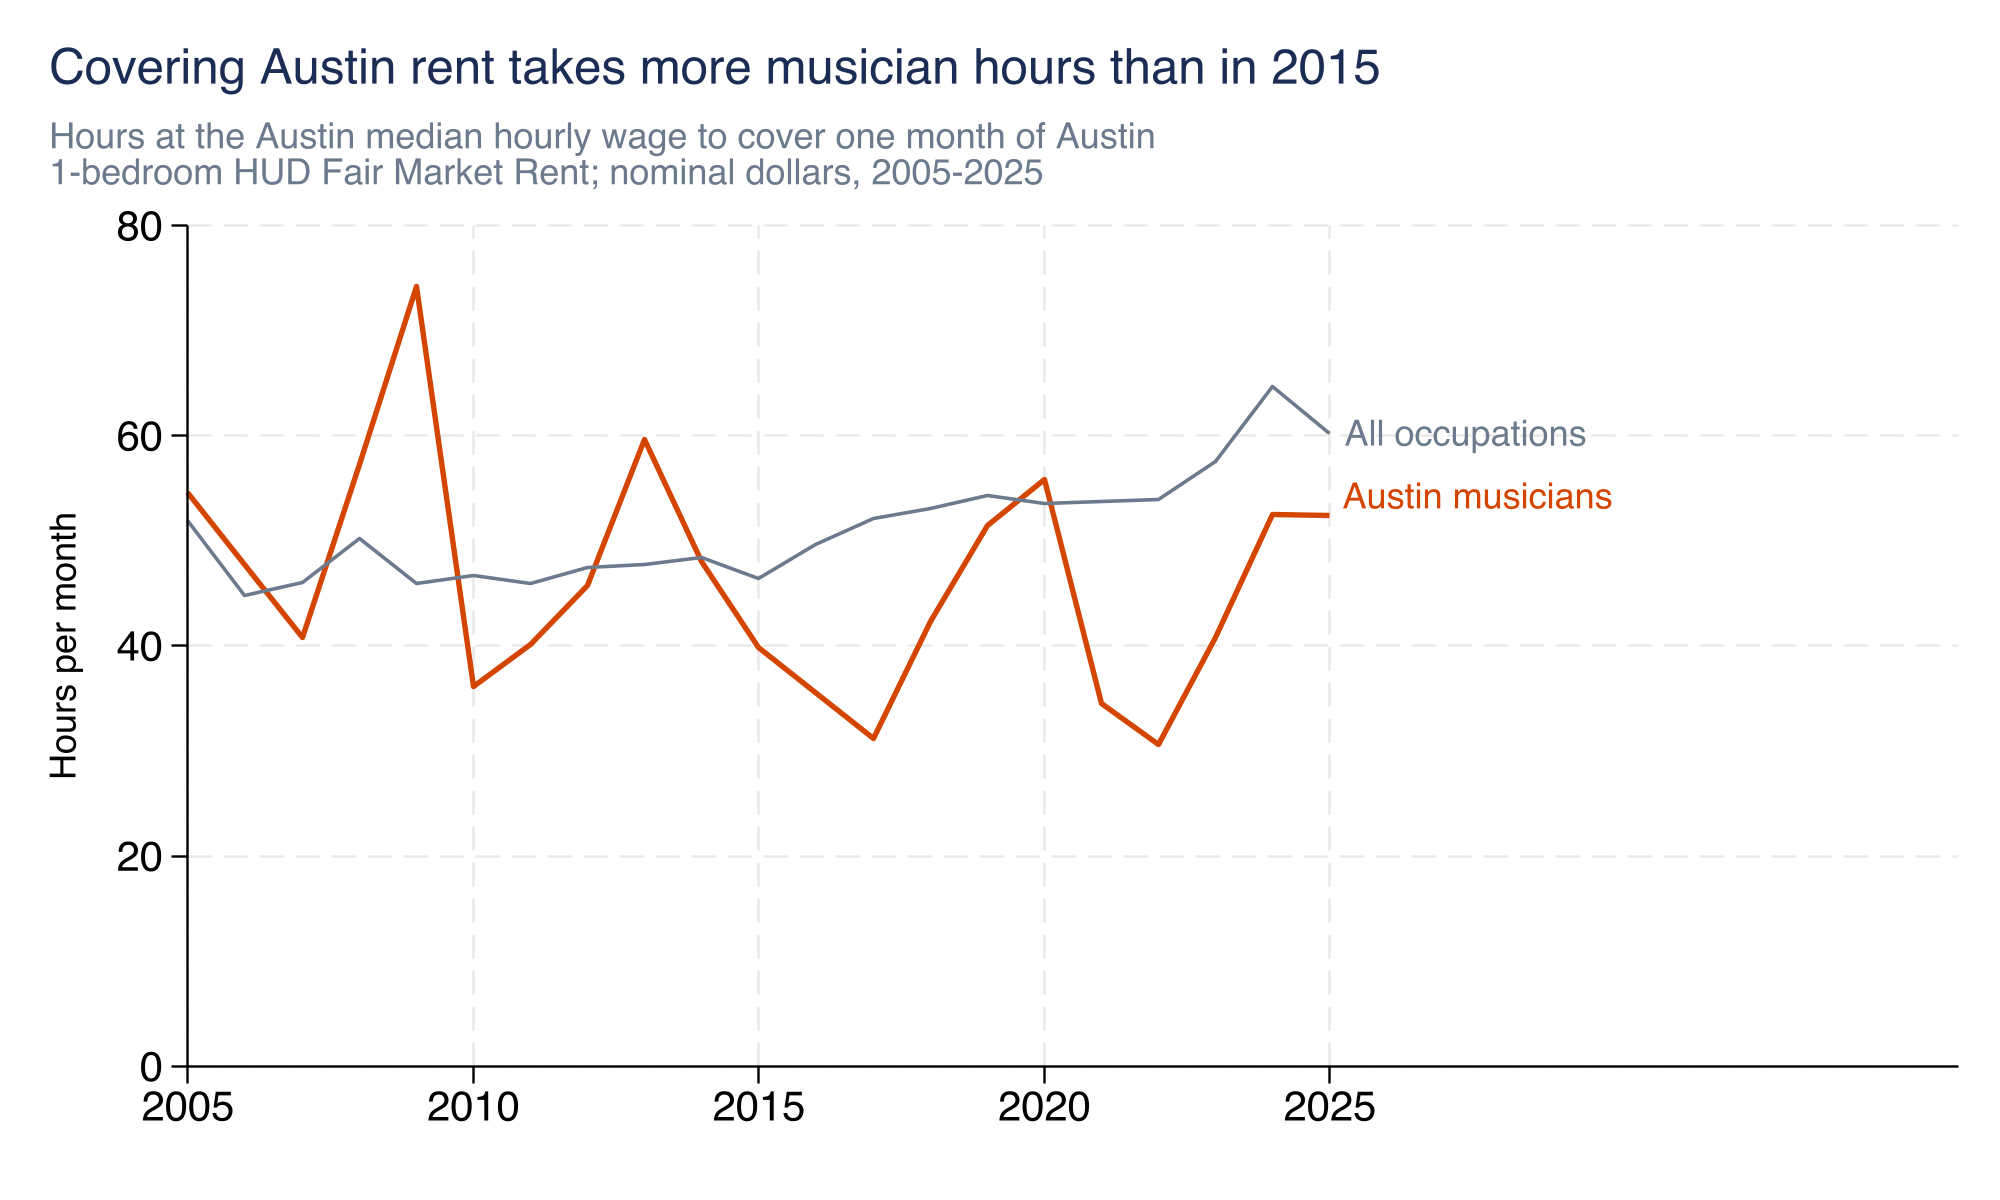
\includegraphics[width=\textwidth]{fig19_rent_vs_wages.png}
\caption{Hours of work at the median hourly wage needed to cover one month of
Austin one-bedroom Fair Market Rent. Sources: Bureau of Labor Statistics
Occupational Employment and Wage Statistics for the Austin metro; HUD Fair
Market Rents; and the City of Austin's purchased earnings series, dataset
\texttt{2qxc-8cme}. Wages and rents are matched within year in nominal terms,
because the ratio of two same-year dollar figures needs no inflation
adjustment. How to read it: a higher line means rent costs more hours of work.
Critical caveat: the federal wage series counts payroll jobs only and excludes
the self-employed, who are \NPumsAustinMusSelfemp\
(\NPumsAustinMusSelfempMoe) of employed Austin-metro musicians aged 18 to 64
over 2020 to 2024, and the Austin musician estimate rests on between about
100 and 700 payroll jobs depending on the year, and
\NEmpPayrollMusiciansAustinLast\ in 2025, which makes it volatile from year to
year. The city's own purchased earnings series, which appears to include
self-employment income, exists for only two years and is not plotted; in 2017
it put musician pay at \NColAnchorCityWageVsOewsTwoZeroOneSeven\ of the
federal figure for the same occupation.}
\label{fig:rentwages}
\end{figure}

The federal payroll wage this figure divides into rent is the Austin-metro
median hourly wage in the BLS Occupational Employment and Wage Statistics
program (OEWS), a semi-annual establishment survey that BLS and the state
workforce agencies run jointly.\footnote{BLS publishes the OEWS Austin
Metropolitan Statistical Area estimates in its annual tables at
\url{https://www.bls.gov/oes/tables.htm}, the most recent vintage being
May~2025. Establishments in the sample report the wage of every worker on
their payroll but report nothing for the self-employed, who fall outside the
sampling frame, so the Austin musician wage in this figure describes only the
\NEmpPayrollMusiciansAustinLast\ musician jobs the 2025 OEWS Austin sample
found on a payroll, and Section~\ref{sec:measurement} develops that
measurement gap in full. BLS does not publish an \emph{annual} musician wage
for any city or year because musician work is too irregular to annualise from
an hourly rate, so the ratio here uses the hourly median.} On that payroll
wage, a month of one-bedroom rent costs an Austin musician
\NColAnchorHoursMusicianLatest\ of work, against
\NColAnchorHoursAlloccLatest\ for the median Austin worker in 2025
(Figure~\ref{fig:rentwages}).\footnote{The ratio is
\(h_{o,y} = F_y / w_{o,y}\), where \(F_y\) is the Austin one-bedroom HUD Fair
Market Rent for fiscal year \(y\) in dollars per month, \(w_{o,y}\) is the
Austin-metro OEWS median hourly wage for occupation group \(o\) in the same
year in dollars per hour, and \(h_{o,y}\) is therefore in hours per month.
This ratio needs no inflation adjustment, and both sides are left in nominal
dollars on purpose: multiplying numerator and denominator by the same factor
\(d_y\) leaves \((d_y F_y)/(d_y w_{o,y}) = F_y / w_{o,y}\), so deflating would
change nothing except to invite a mismatch of years. The two sides are
matched within year for the same reason. BLS did not publish the musician
wage for 2016 and the figure draws a straight segment across that year, so
the 2015-to-2017 stretch of the orange line should not be read as an observed
path. This is a ratio of two published medians, not a sample estimate, so
it has no standard error; its year-to-year movement still reflects sampling
noise in the thin musician wage estimate underneath it.} By that measure
Austin musicians look better placed than the typical Austin worker, because
the OEWS payroll wage covers only the \NEmpPayrollMusiciansAustinLast\
musician jobs the 2025 OEWS Austin sample recorded, the measurement gap
Section~\ref{sec:measurement} describes, and those payroll jobs pay above the
Austin all-occupation median. That ordering is a real feature of the payroll
data and a poor description of the occupation, and on so thin a base the
shape of the orange line across the full period is firmer evidence than the
2025 point on its own.

The picture changes when the earnings measure includes the self-employed. The
Census Bureau's American Community Survey Public Use Microdata Sample (ACS
PUMS) samples households rather than employers, so it captures earnings for
the self-employed alongside payroll earners, at the cost of thinner samples in
any single year.\footnote{The ACS is an ongoing annual household survey the
Census Bureau administers to approximately 3.5 million addresses each year;
the five-year PUMS pools respondents across 2020 through 2024 to produce
metro-level estimates on smaller occupations, at
\url{https://www2.census.gov/programs-surveys/acs/data/pums/2024/5-Year/}. The
Austin-metro musician cell used here is Musicians and Singers (occupation
code OCCP 2752), employed 18 to 64 with positive earnings, weighted by PWGTP.
Because the five-year file is one pooled cross-section rather than five
annual observations, this share is a point estimate for the pooled period
rather than a series that can be plotted year by year.} Measured against ACS
median earnings from Section~\ref{sec:earnings}, a year of one-bedroom HUD
Fair Market Rent would equal \NColPumsRentShareMatched\ of the median annual
earnings of employed Austin-metro musicians aged 18 to 64 over 2020 to
2024.\footnote{The share is
\(s = 100 \times 12\bar{F} \big/ \tilde{y}\), where \(\bar{F}\) is the
average Austin one-bedroom HUD Fair Market Rent across fiscal years 2020 to
2024 in 2025 dollars, the same five years the microdata pool, and
\(\tilde{y}\) is the weighted median personal earnings from work of Austin
musicians in 2025 dollars on the positive-earnings base. Averaging the five
fiscal years rather than picking one is what makes the numerator and the
denominator cover the same period. The numerator is a housing cost for a
dwelling and the denominator is one person's earnings, so \(s\) is
affordability arithmetic rather than an observed housing outlay, and it
carries the margin of error of the earnings median in its denominator.
Measured against the FY2026 rent, which replaces \(\bar{F}\) with that single
year, it is \NColPumsRentShareLatest. Both are far above the 30 percent share
the federal government treats as the ceiling for a rental burden a household
can carry without cost-burden status, which is a statement about arithmetic
rather than a claim about any individual's housing.} The numerator here is a
benchmark rent rather than an observed one. Separate corroboration comes from
Section~\ref{sec:earnings}, which reports that across Texas, renting
households with a musician in them pay a higher median gross rent than
renting worker households generally, while carrying about the same
rent-to-income burden. On that evidence, Texas musician households are not
renting more cheaply than other working households.

\subsection{Real market rents fell while the nominal assistance benchmark kept climbing through 2025}

Figure~\ref{fig:metrorent} shows real rents falling. Figure~\ref{fig:rentwages}
shows hours of work per month of rent rising between 2023 and 2025. Both are
correct, and a reader who noticed the tension without an explanation would be
right to distrust what follows. The two figures rest on different rents and
different denominators, as the table below sets out:

\begin{center}
\footnotesize
\begin{tabular}{@{}B{2.9cm} P{6.3cm} P{6.6cm}@{}}
\toprule
& \textbf{Figure~\ref{fig:metrorent}} & \textbf{Figure~\ref{fig:rentwages}} \\
\midrule
Rent measure & Zillow Observed Rent Index, a market listings series deflated
to constant 2025 dollars and indexed to each metro's own January 2015 level &
HUD Fair Market Rent for a one-bedroom in Austin, nominal dollars, the annual
benchmark for federal housing-assistance payments \\
\rowrule
Wage denominator & None: the line plots rent alone & The BLS OEWS median
hourly wage across the \NEmpPayrollMusiciansAustinLast\ Austin musician jobs
recorded in 2025 \\
\rowrule
Direction, 2023 to 2025 & Down: Zillow market rents fell in real terms in
Austin more than in any other metro compared & Up: HUD's benchmark kept
climbing while the OEWS musician wage fell back from an unusually high 2022
reading \\
\bottomrule
\end{tabular}
\end{center}

\vspace{3pt}
Where this study needs a single number for what renting costs in Austin, it
takes the Zillow market series and says so. The hours-of-rent figure also
rests on an OEWS payroll wage that describes fewer musician jobs than it once
did, and Section~\ref{sec:payroll} follows that count across twenty years.

% Section 4: the shift from payroll to self-employment, seen in two federal
% series that count different things. The honesty constraint is not to present
% them as one workforce total.
\section{Payroll music jobs have fallen; solo creative businesses have risen}
\label{sec:payroll}

The Bureau of Labor Statistics has counted fewer payroll musician jobs in Texas
every survey vintage since 2005, and higher real hourly wages for the jobs that
remain.\footnote{The Occupational Employment and Wage Statistics program
(OEWS) is a semi-annual establishment survey the U.S.\ Bureau of Labor
Statistics runs jointly with each state workforce agency. Sampled employers
report the occupation and wage of every worker on their payroll; a
self-employed musician, a musician paid off the books, and a musician
performing under an independent-contractor arrangement never enter the
sampling frame at all. This section therefore reads OEWS as a payroll-only
ceiling on measured wage-and-salary music work rather than as a count of the
workforce. Program documentation at \url{https://www.bls.gov/oes/oes_ques.htm};
the tables read here are the May 2005 through May 2025 state and metropolitan
estimates for Musicians and Singers, Standard Occupational Classification code
27-2042, published at \url{https://www.bls.gov/oes/tables.htm}. BLS does not
publish an annual wage for this occupation in most cells because the work is
too irregular to annualise from an hourly rate.} On its own that pattern reads
as an occupation getting smaller and better paid. Set against the household
microdata in Section~\ref{sec:earnings}, a second reading opens: the same
work has moved out of payroll and into self-employment, which no payroll
wage series covers. The last subsection here tests that reading against the
timing of the two series and finds it weaker than a first look suggests.

In Texas, OEWS records \NEmpPayrollMusiciansTxFirst\ payroll musician jobs in
2005 and \NEmpPayrollMusiciansTxLast\ in 2025, a change of
\NEmpPayrollPctchgMusiciansTx\ over twenty years. The same program records a
national change of \NEmpPayrollPctchgMusiciansUs\ over the same window. For
the payroll jobs that remained in Texas, the real median hourly wage rose
\NWageHourlyPctchgMusiciansTx, from \NWageHourlyRealMusiciansTxFirst\ in 2005
to \NWageHourlyRealMusiciansTxLast\ in 2025, both in 2025 dollars
(Figure~\ref{fig:wagetrend}).\footnote{Every percentage change quoted in
this section is an endpoint change over the whole span,
\(100\,(X_T / X_0 - 1)\), where \(X_0\) is the first year with a published
value and \(X_T\) the last, so it is not an annual rate and it says nothing
about the path between the two years. Job counts are compared as published,
because a count of jobs is not a dollar figure and nothing in it needs
deflating. The wage is deflated before it is differenced,
\(w^{\mathrm{real}}_y = w_y \times d_y\) with \(d_y = C_{2025}/C_y\) the ratio
of national consumer price index annual averages, so the change reported here
is the change in purchasing power and not the change in the posted wage. Where
a series has no published value for a year, the endpoints move inward to the
first and last years that do, which for the Austin musician wage shortens the
window. These are the OEWS program's own published medians and counts; BLS
publishes no margin of error for these cells, so none is shown.}

\begin{figure}[htbp]
\centering
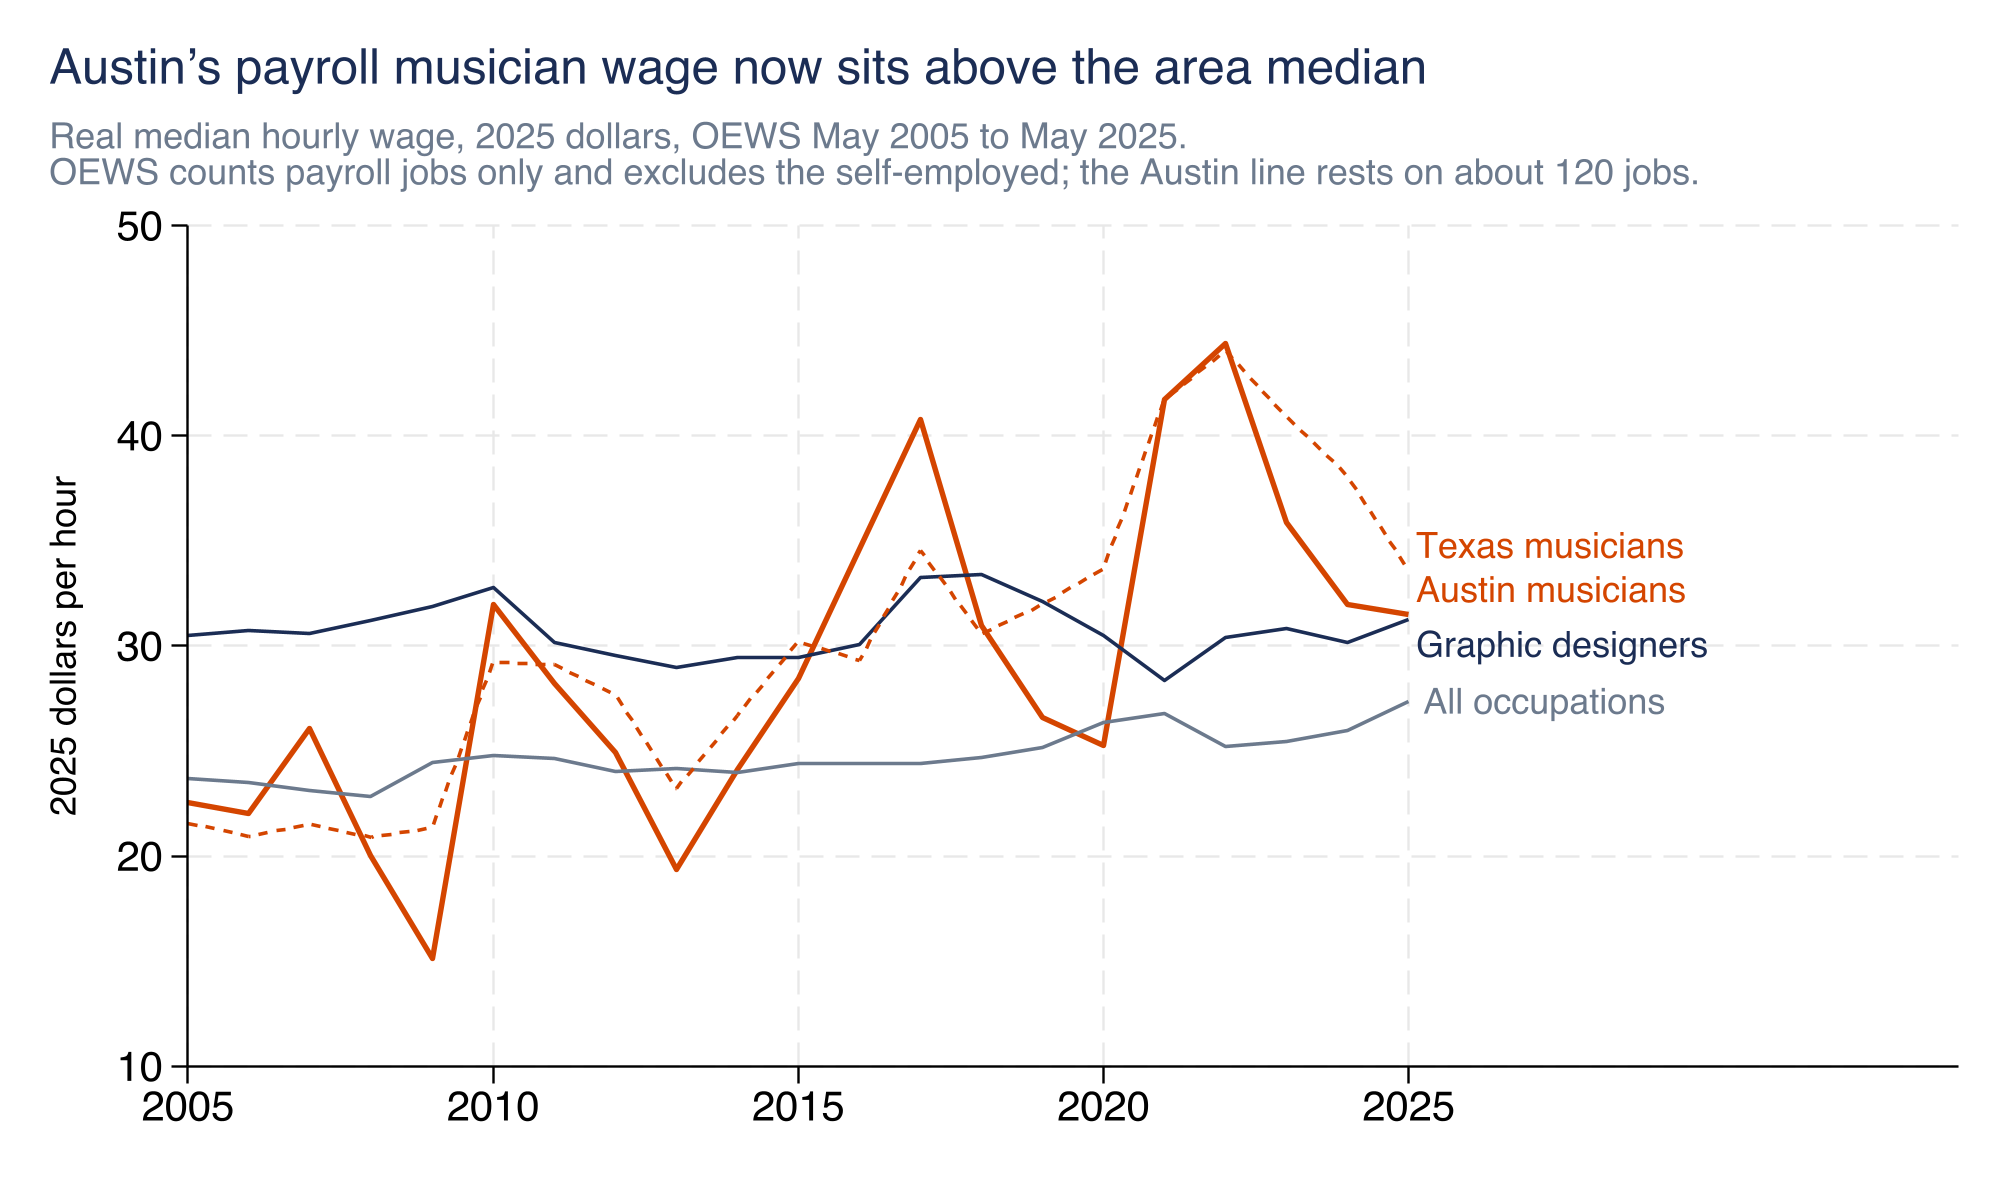
\includegraphics[width=\textwidth]{fig07_real_wage_trend.png}
\caption{Real median hourly wage for selected occupations, Austin metro and
Texas, 2005--2025, in 2025 dollars. Source: U.S.\ Bureau of Labor Statistics,
Occupational Employment and Wage Statistics, May 2005 through May 2025 tables
for Musicians and Singers (SOC 27-2042), deflated with the national consumer
price index (CPI-U, annual average). How to read it: the axis does not start
at zero. The Austin musician line swings widely because it rests on between
about 100 and 700 payroll jobs depending on the year, so movements of several
dollars between years reflect sampling variation rather than changes in what
Austin musicians are paid. Caveat: OEWS excludes the self-employed by design,
so this series describes a small and better-paid slice of the occupation
rather than the occupation itself.}
\label{fig:wagetrend}
\end{figure}

\subsection{Solo creative businesses grew while payroll music jobs fell}

The U.S.\ Census Bureau publishes a separate account of solo creative work
through Nonemployer Statistics, an administrative tabulation the Bureau builds
from federal tax filings rather than from a survey.\footnote{Nonemployer
Statistics counts business establishments with no paid employees and at least
one thousand dollars of annual receipts (one dollar in construction), drawn
from the Internal Revenue Service's business tax records: Form 1040 Schedule C
for sole proprietors, Form 1065 for partnerships, and the corporate returns
1120 and 1120S. The sampling frame is therefore tax filings, not households
or payrolls, so the file captures registered solo businesses that OEWS
structurally cannot see but omits cash gig work that never enters the tax
record. The industry code used here, NAICS 7115, is Independent Artists,
Writers, and Performers, a category broader than musicians alone. County-level
release: \url{https://www2.census.gov/programs-surveys/nonemployer-statistics/datasets/2023/historical-datasets/nonemp23co.zip}.
Program documentation:
\url{https://www.census.gov/programs-surveys/nonemployer-statistics.html}.
The Census Bureau protects county cells with noise infusion, adding small
random errors to published values instead of suppressing them, which matters
more for a county cell than for a state one.} That series counts a different
unit (a solo business, not a job) over a different universe (all independent
artists, writers and performers, not musicians alone) than OEWS. The two
files are therefore not additive, and Figure~\ref{fig:substitution} draws
them as separate panels so no reader adds them.

\begin{figure}[htbp]
\centering
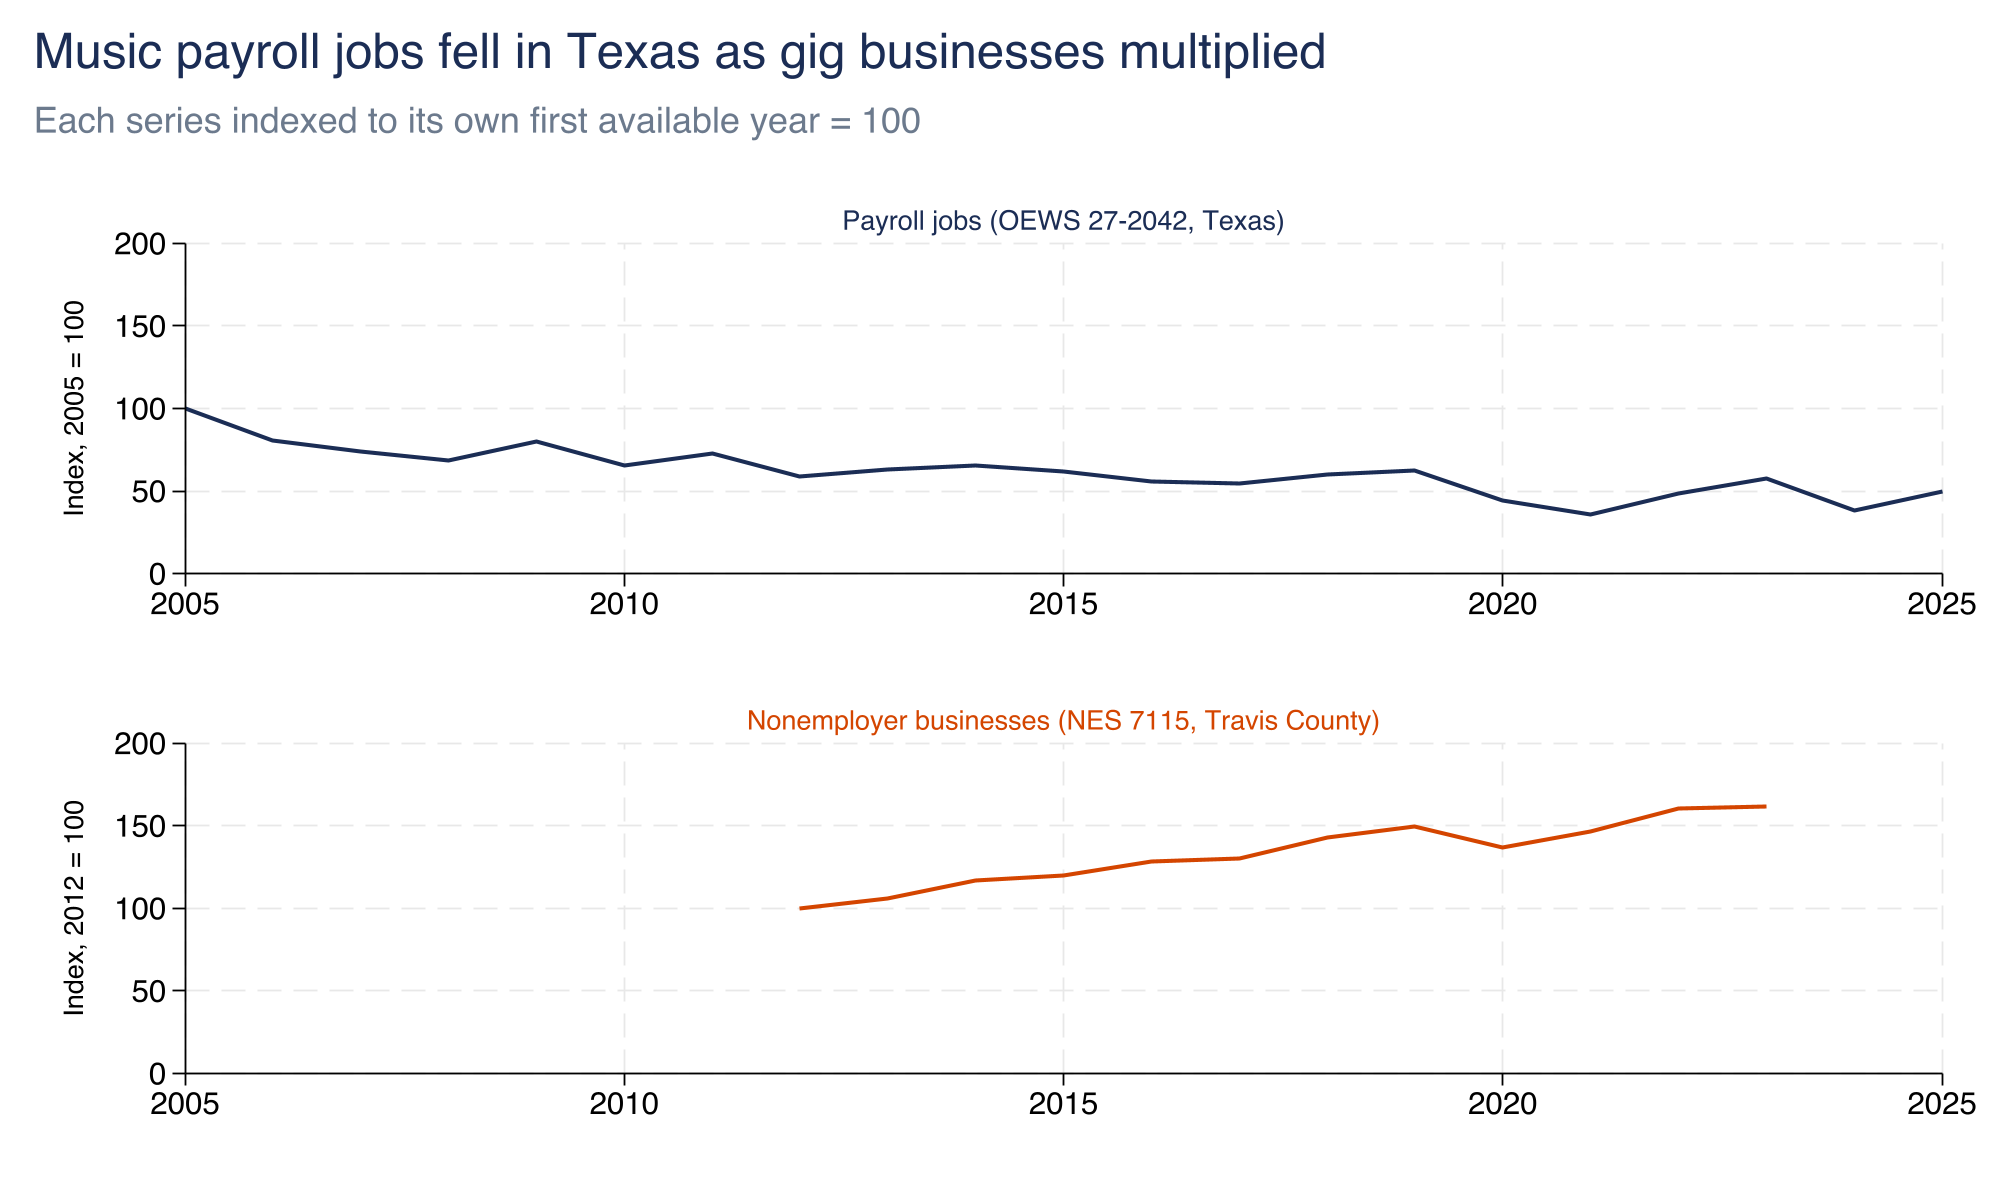
\includegraphics[width=\textwidth]{fig06_payroll_vs_nonemployer.png}
\caption{Payroll music jobs against independent-artist businesses without
employees, each indexed to its own first available year. Sources: U.S.\
Bureau of Labor Statistics, OEWS, for payroll employment in Musicians and
Singers (SOC 27-2042); U.S.\ Census Bureau, Nonemployer Statistics, for
establishments in NAICS 7115 (Independent Artists, Writers, and Performers).
How to read it: the two series count different things over different
universes, jobs against businesses and musicians against all independent
artists, so the figure shows the direction each is moving and nothing more.
The panels must not be added or netted.}
\label{fig:substitution}
\end{figure}

Nonemployer establishments in NAICS 7115 rose
\NSubstitutionNonemployerTravisPctchg\ in Travis County between 2012 and
2023 and \NSubstitutionNonemployerTxPctchg\ across Texas over the same
window.\footnote{Nonemployer Statistics reports Travis County
establishments in NAICS 7115 at 5{,}382 in 2012 and 8{,}696 in 2023, and
Texas statewide at 45{,}021 and 74{,}834 over the same years. Both figures
are business counts, not people, and the Bureau's noise-infusion procedure
means a single county cell has a slightly larger measurement error than the
state total.} Texas payroll music jobs, measured over their own longer OEWS
window of 2005 to 2025, changed
\NEmpPayrollPctchgMusiciansTx.\footnote{Figure~\ref{fig:substitution}
rebases each series on its own first available year,
\(I_{s,t} = 100 \times X_{s,t} / X_{s,t_0(s)}\), where \(X_{s,t}\) is the
level of series \(s\) in year \(t\) and \(t_0(s)\) is that series' first
year: 2005 for OEWS payroll jobs, 2012 for the Nonemployer Statistics
establishment count. Rebasing is what allows two series measured in
different units, jobs in one case and businesses in the other, to sit on a
common vertical scale, and it is also the reason the two panels cannot be
added or netted: an index number carries no unit and no count, only a
direction and a rate of movement relative to its own starting point.} These
two series do not count the same people. This study makes no estimate of
the total size of the Austin music workforce, because no public source
supports one.

Among the four large Texas counties compared here, Travis County has the
highest rate of independent-artist businesses relative to its population:
\NNesEstabPerOneZerokTravisTwoZeroTwoThree\ nonemployer establishments in
NAICS 7115 per 10{,}000 residents in 2023, against
\NNesEstabPerOneZerokDallasTwoZeroTwoThree\ in Dallas,
\NNesEstabPerOneZerokBexarTwoZeroTwoThree\ in Bexar and
\NNesEstabPerOneZerokHarrisTwoZeroTwoThree\ in Harris
(Figure~\ref{fig:metrones}).\footnote{The rate is
\(10^{4} \times E_{c,y} / N_{c,y}\), where \(E_{c,y}\) is the count of
Nonemployer Statistics establishments in NAICS 7115 in county \(c\) and
year \(y\), and \(N_{c,y}\) is that county's resident population in the
same year, taken from the U.S.\ Census Bureau's Vintage 2025 Population
Estimates Program release
(\url{https://www2.census.gov/programs-surveys/popest/datasets/2020-2025/counties/totals/}).
Both sides share a year, so the measure is a rate rather than a count and
counties of different sizes can sit beside one another. The numerator
counts businesses and not people, and one person can hold more than one,
so this rate is a proxy for how common solo creative work is rather than
a headcount of solo creatives. Four of Texas's 254 counties appear here,
so the ranking is bounded by those four.}

\begin{figure}[htbp]
\centering
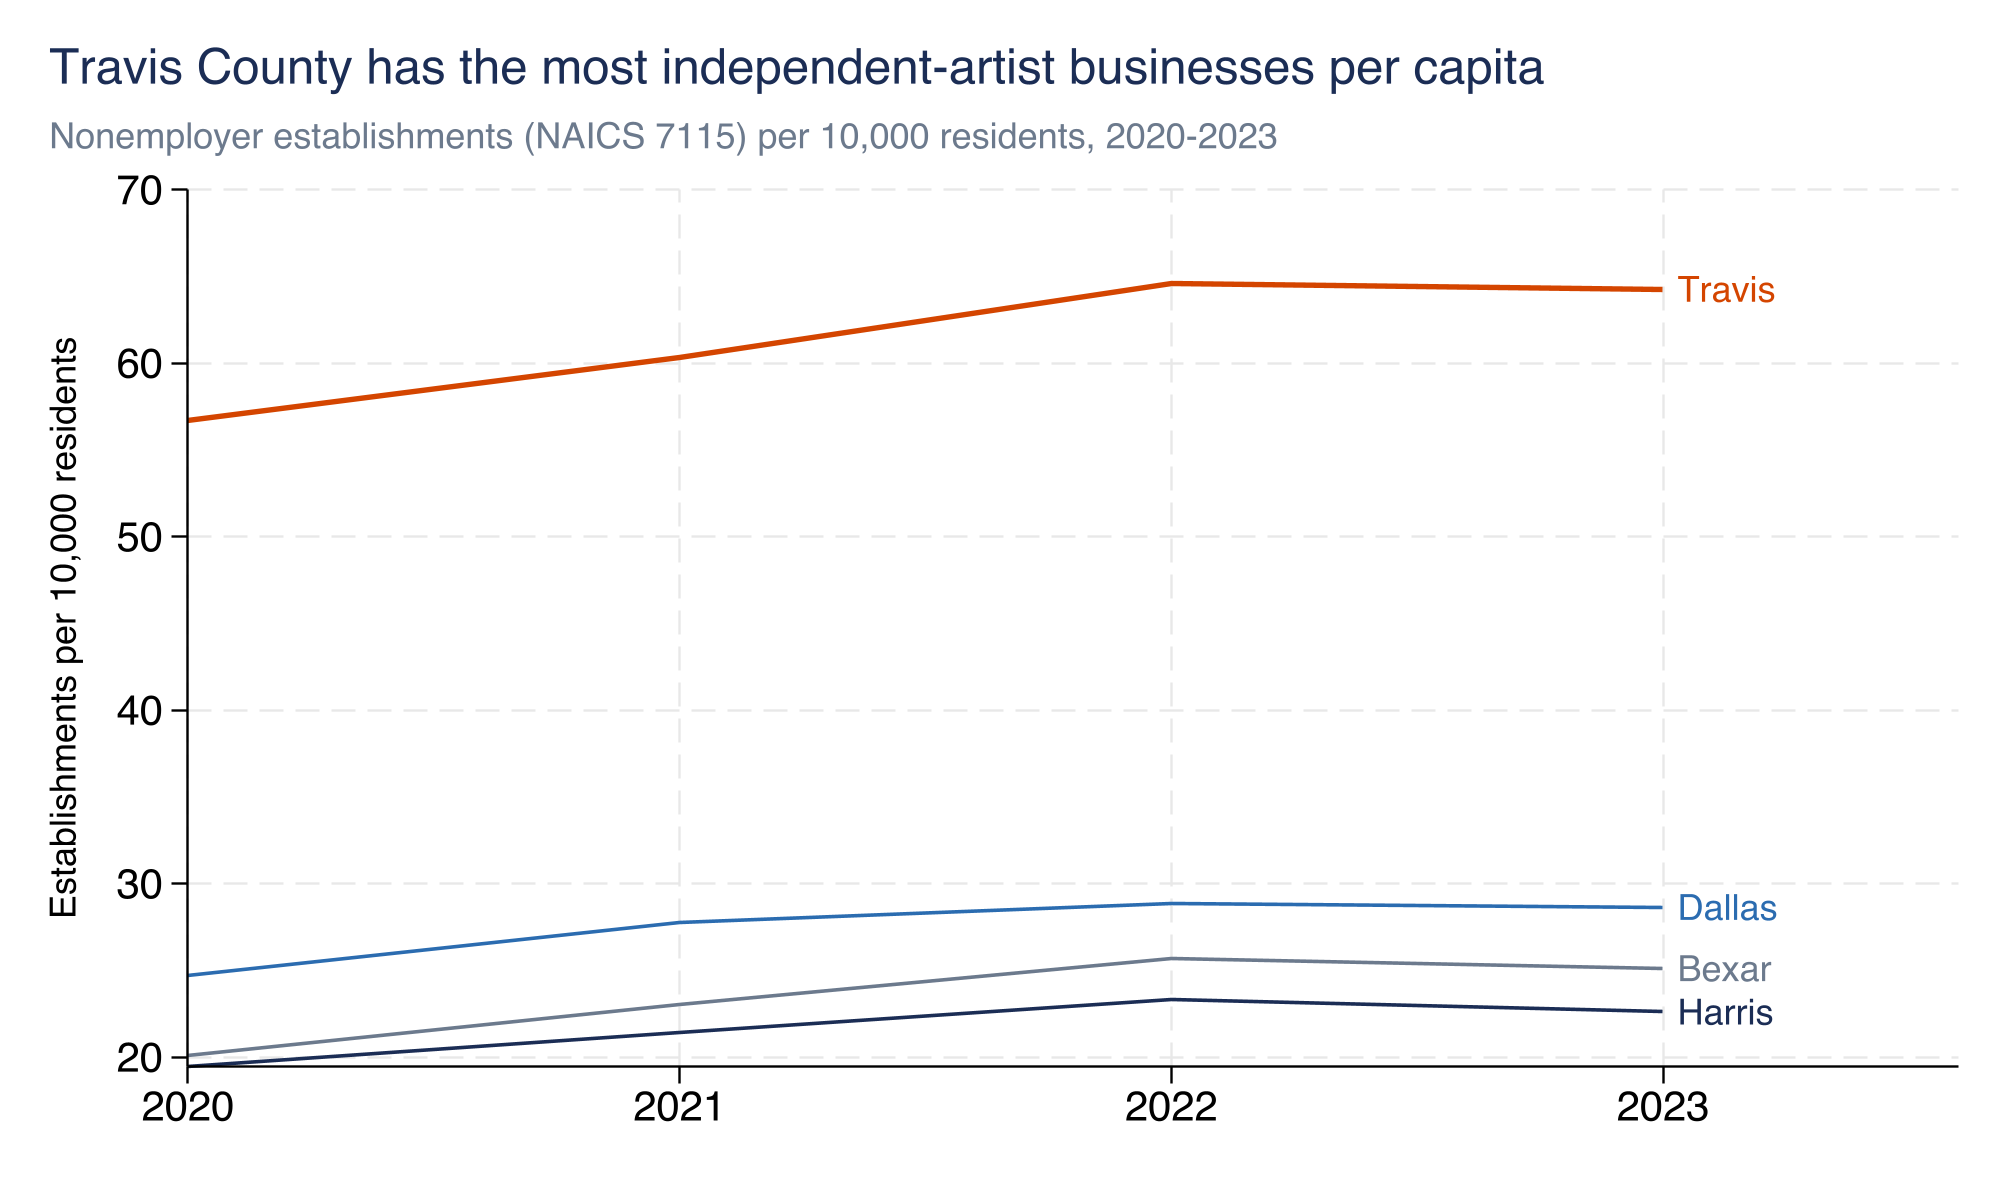
\includegraphics[width=0.86\textwidth]{fig08_metro_nonemployer.png}
\caption{Independent-artist businesses without employees per 10,000
residents, four Texas counties, 2020--2023. Sources: U.S.\ Census Bureau,
Nonemployer Statistics, NAICS 7115; county population from the U.S.\ Census
Bureau's Vintage 2025 Population Estimates Program. How to read it: a
higher line means more solo creative businesses relative to population.
Caveats: NAICS 7115 covers independent artists, writers and performers
together, so the count is a proxy for solo creative work rather than a
headcount of musicians; the series is shorter than the 2012--2023
establishment counts because the population denominator comes from the
Vintage 2025 estimates, which do not reach back to 2012; and four of
Texas's 254 counties appear here, so the ranking is bounded by those
four.}
\label{fig:metrones}
\end{figure}

Travis County's concentration of solo creative businesses is real; what
those businesses take in is less clear. Nonemployer Statistics reports
gross receipts before any expense: real receipts per Travis County
establishment in NAICS 7115 rose \NNesReceiptsPerEstabPctchgTravis\
between 2012 and 2023, to
\NNesReceiptsPerEstabTravisLast\ in 2025
dollars.\footnote{Receipts per business is
\(\bar{r}_{c,y} = R^{\mathrm{real}}_{c,y} / E_{c,y}\), where
\(R^{\mathrm{real}}_{c,y}\) is total NAICS 7115 receipts in county \(c\)
and year \(y\), deflated to 2025 dollars by \(d_y = C_{2025}/C_y\), and
\(E_{c,y}\) is the establishment count. This is an arithmetic mean with no
distribution behind it: the Census Bureau publishes only totals and counts
for this category, so a small number of high-earning businesses can carry
the average and no median is available. Noise infusion further complicates
year-to-year comparisons at the county level.} Alongside that receipts
figure sits a separate reading of the cost side of solo music work. The
2022 Greater Austin Music Census, a self-selected online survey of Austin
music workers with no probability sample behind it, asked respondents to
report annual spending on their own music business across eight categories;
the \NCensusSpendCompleteN\ music creatives who answered every one of those
eight categories reported a median of \NCensusSpendTotalMedian\ a year in
2025 dollars.\footnote{Sound Music Cities and City of Austin Music \&
Entertainment Division, \textit{Greater Austin Music Census}, 2022;
respondent-level microdata downloaded from City of Austin open data,
dataset \texttt{an3p-3yqx}, at
\url{https://data.austintexas.gov/}, retrieved 1 August 2026. The
instrument was distributed through music-community mailing lists and city
channels between 15 July and 12 September 2022, drew 2{,}227 respondent
records, and carried no probability weights. The complete-spender base of
\NCensusSpendCompleteN\ is 22.5 percent of respondents; the eight
categories are gear and rentals, publicity and promotion, rehearsal or
work space, new recordings, merchandise, supplies, web and social media,
and accounting and legal. The median above is the median of respondent
totals, not a sum of category medians.} The receipts figure is Census
Bureau administrative data on all Travis County solo businesses in NAICS
7115; the spending figure is a self-selected survey of Austin music
creatives specifically. The two describe different populations in
different years and cannot be subtracted from one another. They sit
together here because a receipts figure alone overstates what a solo
creative keeps.

\subsection{The substitution reading is an inference, not a tracked transition}

The two series do not move in the same years, which weakens the reading
that payroll music jobs became solo creative businesses rather than
supporting it. Most of the Texas OEWS payroll decline happened between 2005
and 2012, and the payroll count has moved sideways since; the Nonemployer
Statistics series begins in 2012, after that fall. What the two files show
together is a payroll count far below its 2005 level and a nonemployer
establishment count that has risen since 2012. Alongside them sits the ACS
PUMS microdata finding that \NPumsAustinMusSelfemp\
(\NPumsAustinMusSelfempMoe) of Austin musicians worked for themselves over
2020 to 2024, which is a single pooled cross-section from a household
survey and carries no time path of its own.\footnote{Musicians and Singers
(OCCP 2752), Austin-Round Rock-San Marcos metro, ages 18--64, employed
(ESR 1/2/4/5), classified self-employed if Class of Worker equals 6
(unincorporated) or 7 (incorporated), from the U.S.\ Census Bureau's
American Community Survey 2020--2024 five-year Public Use Microdata
Sample for Texas
(\url{https://www2.census.gov/programs-surveys/acs/data/pums/2024/5-Year/csv_ptx.zip}).
The share rests on 77 unweighted records; the margin of error uses the
Bureau's successive-difference replication method against the 80
replicate weights.} No public dataset follows individual musicians across
employment arrangements, so nothing here shows that particular OEWS
payroll jobs became particular Nonemployer Statistics businesses.

What the evidence does establish is narrower and still consequential: the
number of music jobs any payroll statistic can observe is lower now than in
2005, while the count of solo creative businesses in the same broad
category has risen since 2012, so payroll records describe less of Austin's
music work than they once did. No public source estimates what fraction of
Austin's music workforce now sits outside payroll records altogether,
because no source combining the payroll and self-employed sides at the
metro level exists. Section~\ref{sec:venues} turns from workers to
workplaces, and tracks the Austin live-music rooms where those solo careers
are performed, using the state Comptroller's monthly alcohol-tax filings as
a room-level receipts record the payroll surveys cannot supply.

% Section 5: the venue panel, the report's original dataset, plus the
% quasi-experimental tests. The key analytic move is separating the aggregate
% decline (real) from per-venue performance (no different from other bars).
\section{Austin's live-music capacity is shrinking through room loss rather than weaker trade}
\label{sec:venues}

Musicians need places to play, and Austin's rooms are measurable in a way
musicians themselves are not. The Texas Comptroller of Public Accounts collects
a monthly filing from every business in the state holding a mixed-beverage
permit (the state's license to sell liquor by the drink), reports each
location's gross receipts, and publishes the file on the state open data
portal.\footnote{Texas Comptroller of Public Accounts, \textit{Mixed Beverage
Gross Receipts}, Texas Open Data Portal dataset \texttt{naix-2893}, at
\url{https://data.texas.gov/dataset/Mixed-Beverage-Gross-Receipts/naix-2893},
retrieved 2 August 2026. The population is every permittee filing under the
mixed-beverage permit categories (MB, BQ, PE and their subtypes); the file is
refreshed monthly and the extract used here covers obligation end dates January
2007 through August 2026. The dataset omits rooms operating on a beer-and-wine
permit only, and it omits venues without a separable alcohol permit or folded
into a hotel or nonprofit permit, so it undercounts several well-known Austin
listening rooms; the panel construction below inherits those omissions. Every
filing is a legal tax record rather than a survey response, which makes it a
census of the licensed universe rather than a sample of it, and each row carries
the permittee's taxpayer name, the location address and the reported gross
receipts for the month.} This study matches those filings to named venues by
taxpayer name and location address and follows a panel of
\NVenuePanelIsCurated\ Austin live-music rooms monthly from January 2007
through June 2026, tracked across changes of owner and legal name.\footnote{The panel is a
\emph{curated} tracking set of named Austin live-music rooms, not a census of
the licensed universe and not a probability sample of it. Rooms enter by name
identification against a research list of Austin live-music venues, so the panel
over-represents established rooms in the central city (Red River, downtown,
East Austin and South Congress), and it excludes venues without a separable
liquor permit, which removes several well-known listening rooms including
Cactus Cafe, Bass Concert Hall, Central Presbyterian, Carousel Lounge,
Meanwhile Brewing, Whip In and Geraldine's. Receipts also measure alcohol
sales rather than music activity: a room's mixed-beverage receipts say nothing
directly about what performers were paid, only what the bar took at the register
that month. Ten festival concession venue-months, in which a festival company
filed under a venue-linked entity name for a month at a scale more than three
hundred times the host venue's median month, are excluded from every venue-level
figure that follows and are worth \NVenueFestivalDollarsExcluded\ in nominal
dollars; the citywide totals used for comparison keep them, because there the
money is real Austin licensed-beverage activity and only its venue label is
misleading. The panel is compared against the full Travis County and City of
Austin licensed-beverage universe throughout this section, and each comparison
names the two sides in matching terms.} With that panel this section asks
whether the sector is contracting because surviving rooms trade worse than the
rest of the licensed-beverage market, or because rooms close and no one replaces
them.

\subsection{Receipts fell at live-music rooms while the market around them added locations}

\begin{figure}[htbp]
\centering
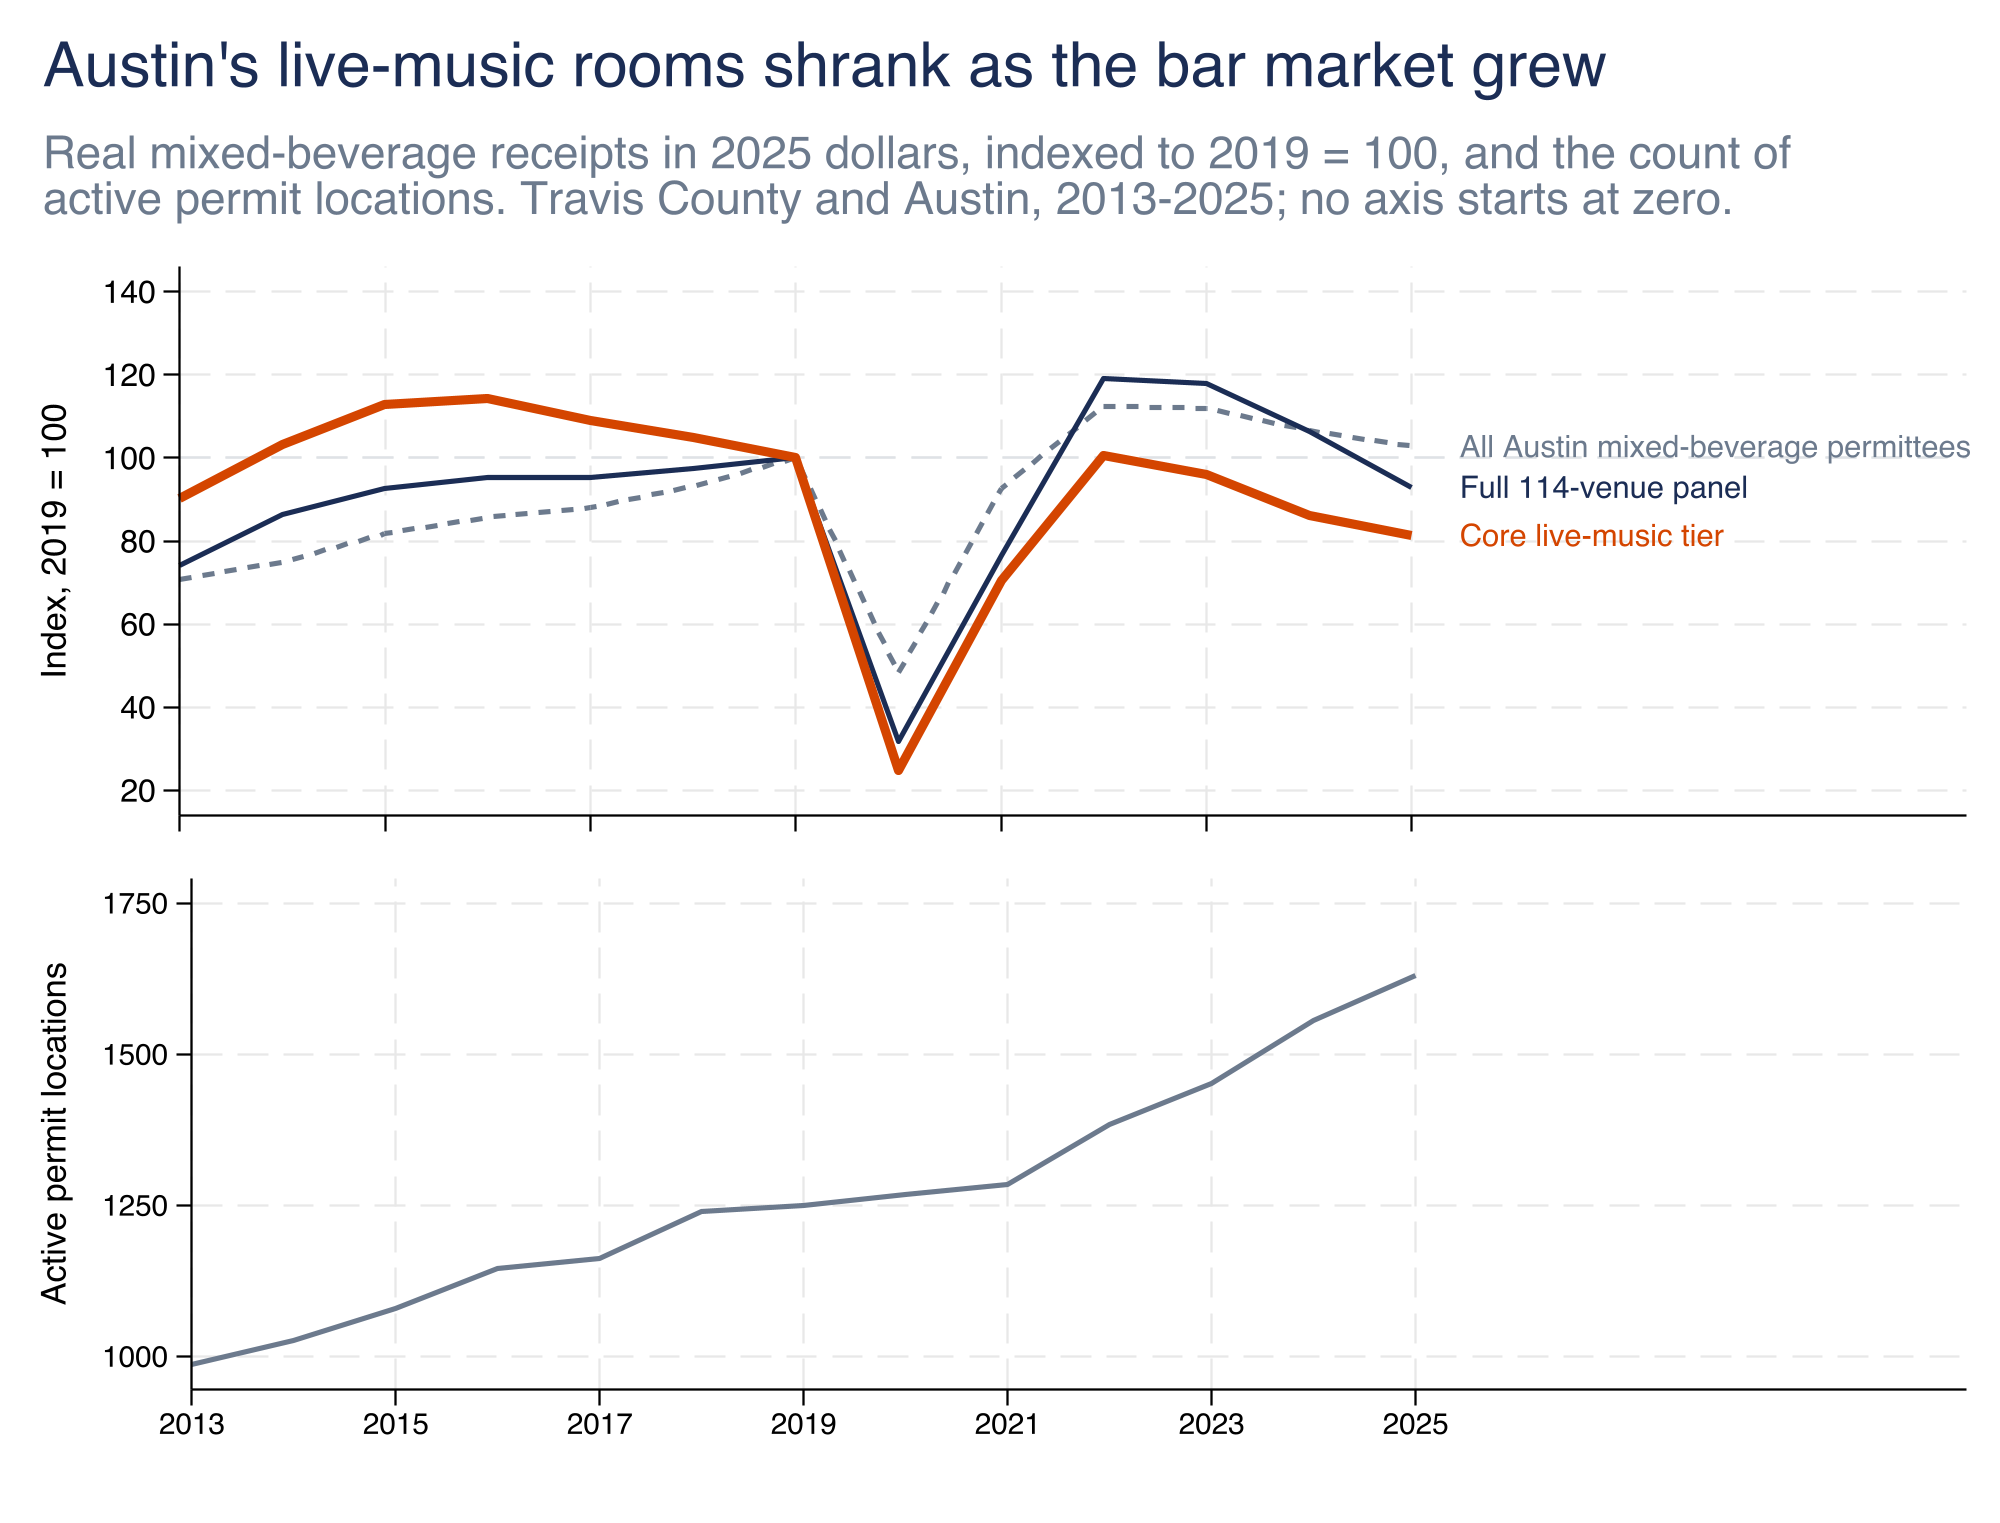
\includegraphics[width=\textwidth]{fig09_venue_receipts_index.png}
\caption{Real mixed-beverage receipts indexed to 2019, and the count of active
permit locations, Travis County and City of Austin, 2013--2025, 2025 dollars.
Source: Texas Comptroller of Public Accounts, \textit{Mixed Beverage Gross
Receipts}, Texas Open Data Portal dataset \texttt{naix-2893}, matched to named
venues by taxpayer name and location address and deflated with the national
Consumer Price Index for All Urban Consumers (CPI-U, series
\texttt{CUUR0000SA0}). How to read it: the upper panel compares three groups
against their own 2019 level, so all three start at 100 by construction; the
lower panel shows how many distinct permit locations filed receipts in each
year. The three groups are the \NVenuePanelIsCurated-venue curated live-music
panel; its core live-music tier of rooms whose main business is live
performance; and the full Travis County and City of Austin mixed-beverage
universe. Caveat: receipts measure alcohol sales, not attendance, ticket
revenue or what performers were paid; the curated panel is not a census, so it
is smaller and more central than the universe by construction.}
\label{fig:venueindex}
\end{figure}

Real receipts fell between 2019 and 2025 at the rooms the curated panel
tracks: \NVenuePanelPctTwoZeroOneNineTwoZeroTwoFive\ across the
\NVenuePanelIsCurated-room panel and
\NVenueCorePctTwoZeroOneNineTwoZeroTwoFive\ in its core live-music tier, the
rooms whose main business is live performance.\footnote{Every filing is
deflated before anything is added up:
\(R^{\mathrm{real}}_{it} = R_{it} \times d_{y(t)}\), where \(R_{it}\) is venue
\(i\)'s nominal receipts in month \(t\), \(y(t)\) is the calendar year
containing that month, and \(d_y = C_{2025}/C_y\) is the ratio of national
consumer price index annual averages. Group totals are
\(S_{g,y} = \sum_{i \in g} \sum_{t \in y} R^{\mathrm{real}}_{it}\), and the
change quoted is \(100\,(S_{g,2025}/S_{g,2019} - 1)\).
Figure~\ref{fig:venueindex} plots the same totals rebased on 2019,
\(I_{g,y} = 100 \times S_{g,y}/S_{g,2019}\), which is why all three lines
start at 100. These are totals over an unbalanced set of filers, so a group
can fall because rooms closed as well as because open rooms took less; that
distinction is the subject of the next subsection. Restricted to the
\NVenueBalancedN\ venues filing in both years, the change is
\NVenueBalancedPctTwoZeroOneNineTwoZeroTwoFive, and
\NVenueShrankBalancedN\ of them were smaller in real terms in 2025.} The full
Travis County and City of Austin mixed-beverage universe moved in the opposite
direction over the same six years, changing
\NVenueCitywidePctTwoZeroOneNineTwoZeroTwoFive\ in real receipts, and the count
of distinct permit locations filing during the year grew from
\NVenueCitywidePermitsTwoZeroOneNine\ in 2019 to
\NVenueCitywidePermitsTwoZeroTwoFive\ in 2025.\footnote{The two sides of that comparison
are not built alike. The ten festival-aggregation venue-months are stripped out
of every venue-level series but stay in the citywide market total, where the
money is genuine licensed-beverage activity and only its venue label is wrong.
On the same ex-festival basis the citywide change is about +1.6 percent rather
than \NVenueCitywidePctTwoZeroOneNineTwoZeroTwoFive. The citywide total also
absorbs \NVenueCitywidePermitsPctTwoZeroOneNineTwoZeroTwoFive\ more permit
locations over the period, so it is not a per-room comparison; on a common
basis, the tracked panel held \NVenuePanelShareTwoZeroOneNine\ of citywide
receipts in 2019 and \NVenuePanelShareTwoZeroTwoFive\ in 2025.} Austin kept
adding places to drink while its dedicated live-music rooms appeared to
contract. Some live performance may also have shifted toward informal or
non-dedicated settings this alcohol-tax panel cannot observe---coffee shops,
restaurants, and breweries that host occasional acts---which typically pay
performers less and less regularly, and are not where full-time musicians earn
most of their income.

A separate City of Austin administrative record moves the same
direction.\footnote{City of Austin, \textit{Sound Ordinance Permits}, Socrata
dataset \texttt{ryu3-tuin} at
\url{https://data.austintexas.gov/resource/ryu3-tuin.csv}, retrieved 1 August
2026. The Music \& Entertainment Division issues an Outdoor Music Venue (OMV)
permit under City Code Chapter 9-2 to any establishment that presents amplified
sound outdoors, and the by-year counts used here are annual issuances
tabulated from that permit file. The series is independent of the Comptroller
receipts data because it is a city licensing series rather than a state tax
filing, and it moves in the same direction as the receipts panel; that
concurrence is why it is reported here.} The Music \& Entertainment Division
issued \NVenueOmvPeak\ Outdoor Music Venue permits in both 2014 and 2017 at
the series peak and \NVenueOmvTwoZeroTwoFive\ in 2025, a change of
\NVenueOmvPctFromPeak\ from the peak.\footnote{The change is
\(100\,(P_{2025}/P_{\mathrm{peak}} - 1)\), where \(P_y\) is the count of
outdoor music venue permits the City issued in calendar year \(y\). A permit
count is not a dollar figure, so nothing is deflated, and one room can hold
several permits across years, so the series measures permitted outdoor music
activity rather than a count of distinct rooms.}

\begin{figure}[htbp]
\centering
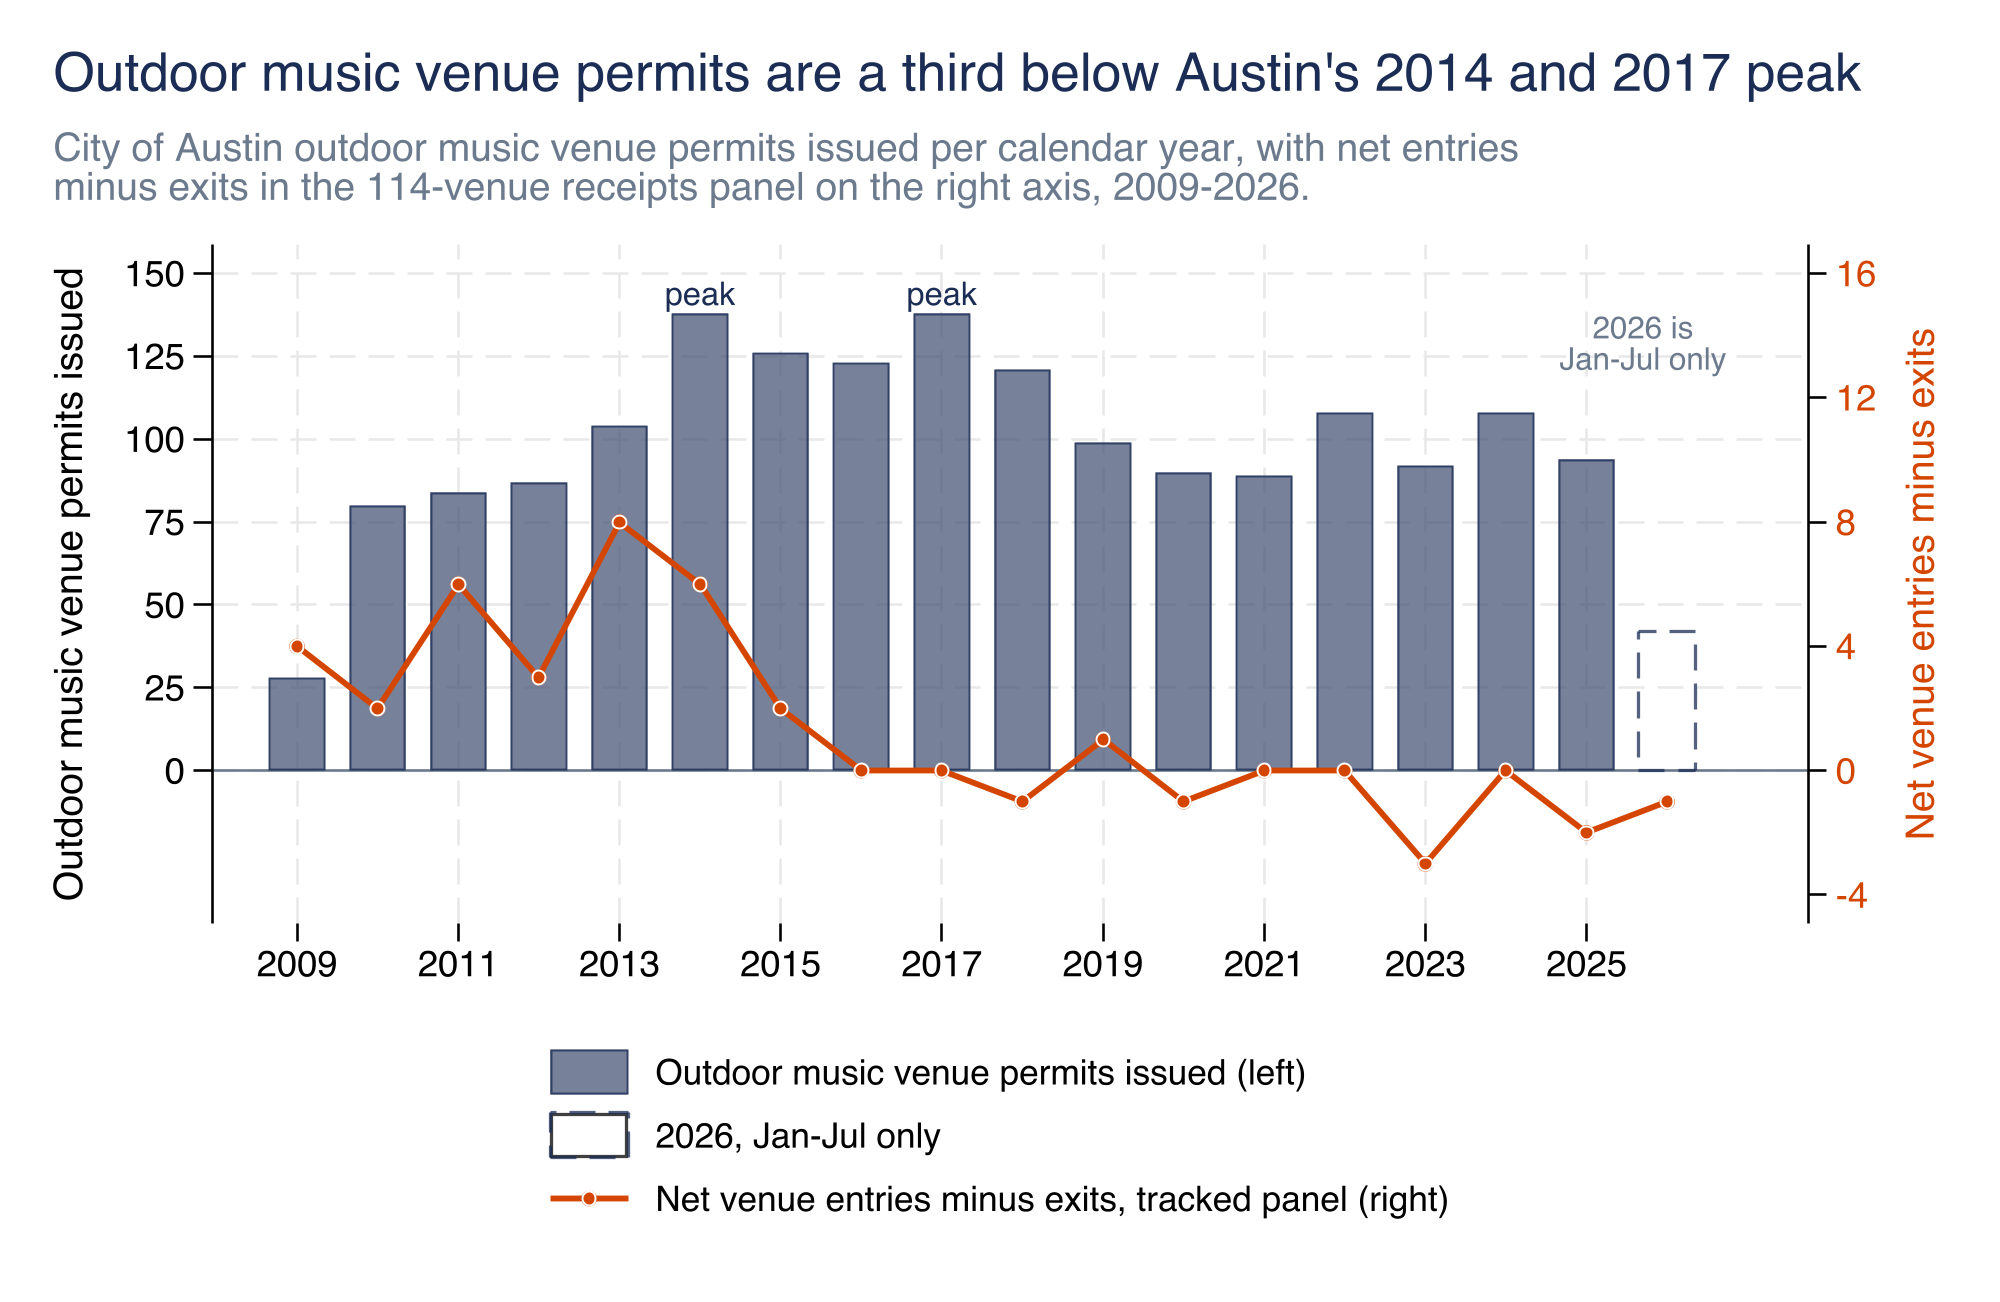
\includegraphics[width=\textwidth]{fig11_venue_supply.png}
\caption{Outdoor Music Venue permits issued by the City of Austin each
calendar year, with net venue entries minus exits in the curated live-music
panel. Sources: City of Austin, \textit{Sound Ordinance Permits}, Socrata
dataset \texttt{ryu3-tuin}; Texas Comptroller of Public Accounts, \textit{Mixed
Beverage Gross Receipts}, dataset \texttt{naix-2893}. How to read it: bars show
permits issued on the left axis and the line shows net additions (entries
minus exits) to the curated \NVenuePanelIsCurated-room panel on the right axis;
the 2026 bar covers only the partial year available at extract. Caveat: a
permit is not a venue, because one room may hold several across years, so the
series measures permitted outdoor music activity rather than a count of rooms.}
\label{fig:venuesupply}
\end{figure}

\subsection{Surviving rooms lost ground, but no more than the rest of the market did}

The aggregate gap invites an obvious explanation, that live-music rooms are
weaker businesses than other bars. Rooms that stayed open did trade down:
among the \NVenueBalancedN\ venues filing in both 2019 and 2025, real receipts
changed \NVenueBalancedPctTwoZeroOneNineTwoZeroTwoFive\ and
\NVenueShrankBalancedN\ shrank. The 2019-to-2025 change by itself cannot tell
whether the surviving live-music rooms fell further than the bars around them
did, because the same 2019-to-2025 change at a citywide comparison group would
carry the same seasonal weather, market-wide inflation and pandemic exposures
that also hit the live-music rooms. The divergence test below strips those
common shocks out, by holding each venue and each calendar month constant, and
asks what is left after both sides have been controlled against themselves.

Comparing the core live-music tier against the rest of the Travis County and
City of Austin mixed-beverage market before and after March 2020, with each
venue and each month held constant, gives an average difference of
\NVenueDidPct, and the 95 percent interval runs from about 14 percent below
the rest of the market to about 17 percent above it (coefficient
\NVenueDidCoef\ log points, clustered standard error \NVenueDidSe, $p =$
\NVenueDidP), across \NVenueDidN.\footnote{The specification is a two-way fixed-effects regression, meaning a
linear regression that includes one intercept for every venue and one
intercept for every calendar month, which together absorb any fixed
characteristic of a room and any month common to the whole market. The
dependent variable is log real monthly receipts, the regressor of interest is
an indicator for core live-music venues interacted with the post-March-2020
period, and standard errors are clustered by venue (that is, they allow the
residuals from the same room to be correlated across months, and treat venues
as the independent units):
\[
\ln R^{\mathrm{real}}_{it}
  = \alpha_i + \tau_t
  + \beta\,\bigl(\mathrm{Core}_i \times \mathrm{Post}_t\bigr)
  + \varepsilon_{it},
\]
where \(R^{\mathrm{real}}_{it}\) is venue \(i\)'s mixed-beverage receipts in
month \(t\) in 2025 dollars; \(\mathrm{Core}_i\) is one for a core live-music
room and zero for other mixed-beverage permit locations in Travis County or the
City of Austin; the panel's live-music-adjacent tier is dropped from the
estimation sample rather than coded zero, because those rooms programme live
music intermittently and belong to neither the treated group nor the
comparison group; \(\mathrm{Post}_t\) is one from March 2020 onward; \(\alpha_i\) is a
venue fixed effect that absorbs everything constant about that room including
its size, address and tier; \(\tau_t\) is a year-month fixed effect that
absorbs everything common to the whole market in that month including the
pandemic, market-wide inflation and season; and \(\varepsilon_{it}\) is the
residual. Only the interaction is estimable, because \(\alpha_i\) absorbs
\(\mathrm{Core}_i\) and \(\tau_t\) absorbs \(\mathrm{Post}_t\). The
interaction is built as an explicit product variable rather than entered
factorially: entered factorially it is collinear with the absorbed effects and
Stata's \texttt{reghdfe} drops the term of interest. Estimation covers
\NVenueDidN\ from January 2013 to December 2025. Months with zero receipts
leave a log specification, so the coefficient describes venues conditional on
trading at all. It converts to a proportional difference as
\(100\,(e^{\hat\beta} - 1)\). This is a descriptive divergence test: no policy
switches on in March 2020 for one group and not the other, and nothing here is
randomised. It is also a precise null rather than an absence of evidence: the
95 percent interval runs from about $-13.7$ to $+16.5$ percent, so a
difference between core live-music rooms and the rest of the mixed-beverage
market much larger than that in either direction is not consistent with these
data.} An event study, which is the same regression with a separate coefficient for
each calendar year rather than one averaged post-March-2020 coefficient, gives
the same reading year by year. Core live-music rooms dropped about 54 log
points below the comparison group in 2020, returned to within statistical
distance of it by 2022, and have tracked it since. The 2019 base is not a
neutral reference, because the pre-2019 coefficients drift upward rather than
sitting flat, so a counterfactual that continued that drift would sit above
zero after 2022 rather than at it.\footnote{The event study replaces the
single interaction with one term per calendar year:
\[
\ln R^{\mathrm{real}}_{it}
  = \alpha_i + \tau_t
  + \sum_{y \neq 2019} \beta_y\,
    \bigl(\mathbf{1}\{\mathrm{year}(t) = y\} \times \mathrm{Core}_i\bigr)
  + \varepsilon_{it},
\]
where \(\mathbf{1}\{\mathrm{year}(t) = y\}\) is one when month \(t\) falls in
calendar year \(y\), 2019 is omitted, and every other symbol, the estimation
sample and the clustering are as in the previous footnote. Each \(\beta_y\)
therefore reads as the gap between core live-music rooms and the rest of the
market in year \(y\), measured against their own 2019 gap, and the 2020 term is
the one quoted above. The year terms are constructed as explicit products with
2019 dropped by hand: asking the estimator to hold 2019 as the base is not
honoured once venue and year-month effects absorb the alternatives, and it
silently renormalises the whole path onto a different year. Pre-2019
coefficients drift upward instead of sitting flat, so parallel trends do not
hold cleanly and the design is descriptive, not causal. A fourth specification
in the exported table replaces the log with the inverse hyperbolic sine, which
keeps zero-receipt months in the sample, and it returns a large negative
coefficient rather than a null; that column answers a different question,
conditioning on nothing rather than on trading, and no number quoted here comes
from it, but a reader should know it points the other way. The full
coefficient path is in the technical appendix.}

If the rooms that stay open trade no worse than other bars, the rest of the
aggregate decline has to come from which rooms exist. \NVenueExitsTotal\ of the
\NVenuePanelIsCurated\ tracked venues had stopped filing altogether by June
2026. \NVenueExitsTwoZeroTwoZeroTwoZeroTwoSix\ of those last filings fall in
2020 or later, and \NVenueExitsTwoZeroTwoZeroTwoZeroTwoSixCore\ of the post-2020
exits were core live-music rooms. Net additions to the panel (entries minus
exits) came to \NVenueNetAddsTwoZeroZeroSevenTwoZeroOneFive\ over 2007--2015 and
\NVenueNetAddsTwoZeroOneSixTwoZeroTwoSix\ over 2016--2026.\footnote{The two
net-add figures are not built alike. The Comptroller receipts file begins in
January 2007, so the 44 venues already trading then all register as 2007
entries; excluding 2007 entirely, the comparable 2008-to-2015 net is +36. The
later figure is not left-censored but is right-truncated at June 2026. Ceasing
to file usually means closure but can also mean a permit transfer, an entity
restructuring, or a switch to a beer-and-wine permit, so these counts are
stopped reporting rather than verified closures.}

\begin{keyfinding}
{\small\textbf{This distinction matters for policy.} Austin's live-music
capacity is contracting because rooms stop filing and are not replaced, while
the wider licensed-beverage market keeps adding permit locations. On
receipts alone, rooms that stayed open trade at the same rate against 2019
as comparable non-music bars; the gap that separates the panel from the
citywide total is not a gap in per-room revenue among survivors. The
receipts file records what bars sell, not what venues spend, so it cannot
say whether operating margins hold; it says only that the aggregate decline
tracks which rooms exist rather than how the open ones sold liquor.}
\end{keyfinding}

Panel venues with lower real receipts in 2025 than in 2019 appear in every
part of Austin the panel can name (Figure~\ref{fig:venuedecline}). The ten
largest dollar declines are concentrated where the panel's own coverage is
concentrated: six sit downtown, on Rainey Street or in the Red River district,
and the other four are in South Austin, in South Central and near the
University of Texas campus. Because dollar size tracks venue size and the
curated panel skews central by construction, that list of ten largest declines
cannot be read as evidence about where decline is or is not spread within the
city.

\begin{figure}[htbp]
\centering
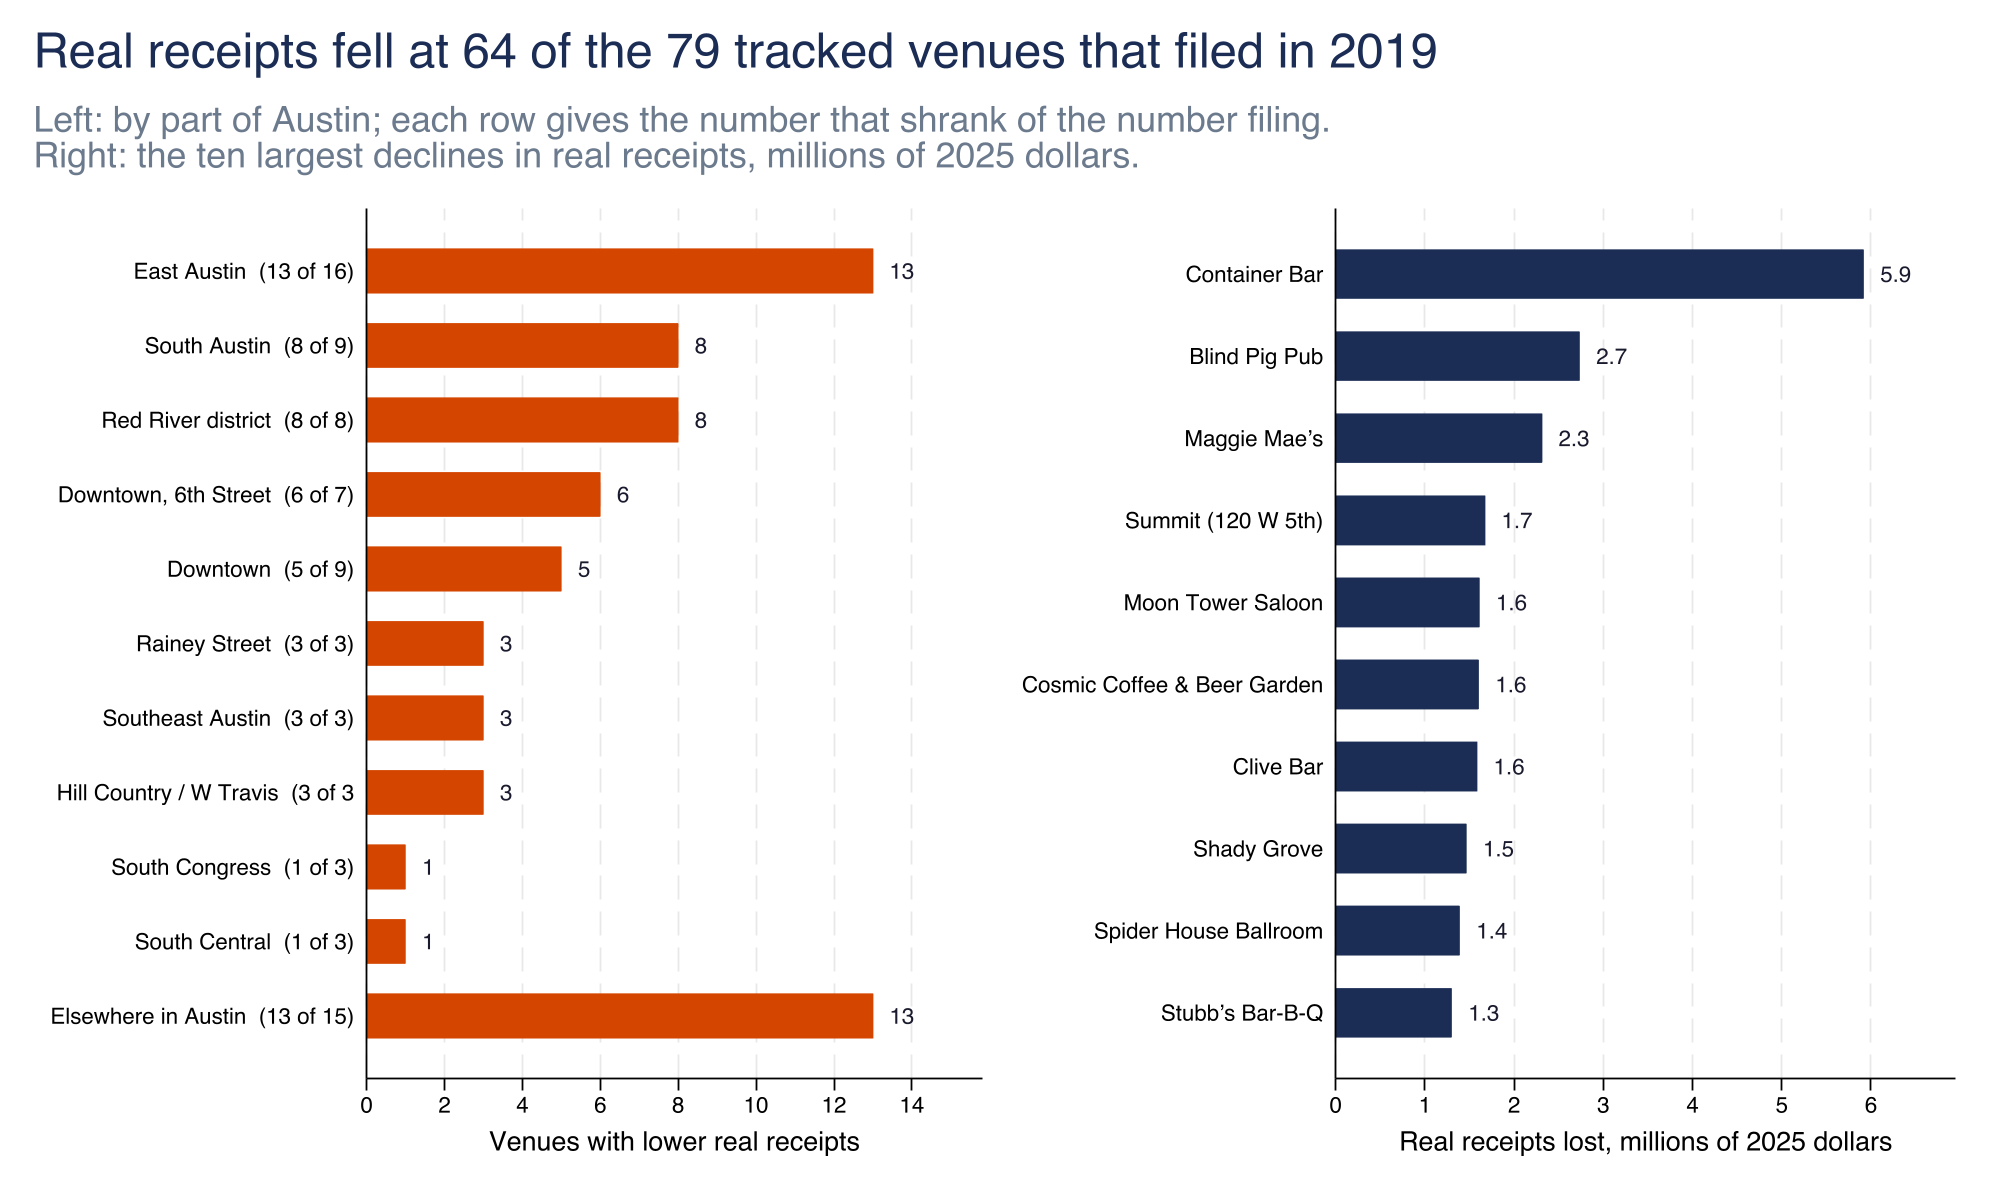
\includegraphics[width=\textwidth]{fig10_venue_map.png}
\caption{Venues in the curated \NVenuePanelIsCurated-room panel with lower
real receipts in 2025 than in 2019, by part of Austin, and the ten largest
dollar declines by venue name. Source: Texas Comptroller of Public Accounts,
\textit{Mixed Beverage Gross Receipts}, dataset \texttt{naix-2893}, deflated
with the national CPI-U. How to read it: each row on the left gives the number
of panel venues that shrank against the number that filed in 2019, so the
denominators differ by area and several rows rest on only three venues; the
right panel shows the size of the ten largest dollar declines by venue name.
Caveats: named parts of Austin are assigned from venue addresses and are
descriptive groupings rather than official boundaries; panel venues that
stopped filing count as zero in 2025 and so appear as declines, which covers 16
of the 64 counted here, and three of the ten largest named declines are rooms
with no 2025 receipts at all.}
\label{fig:venuedecline}
\end{figure}

\begin{figure}[htbp]
\centering
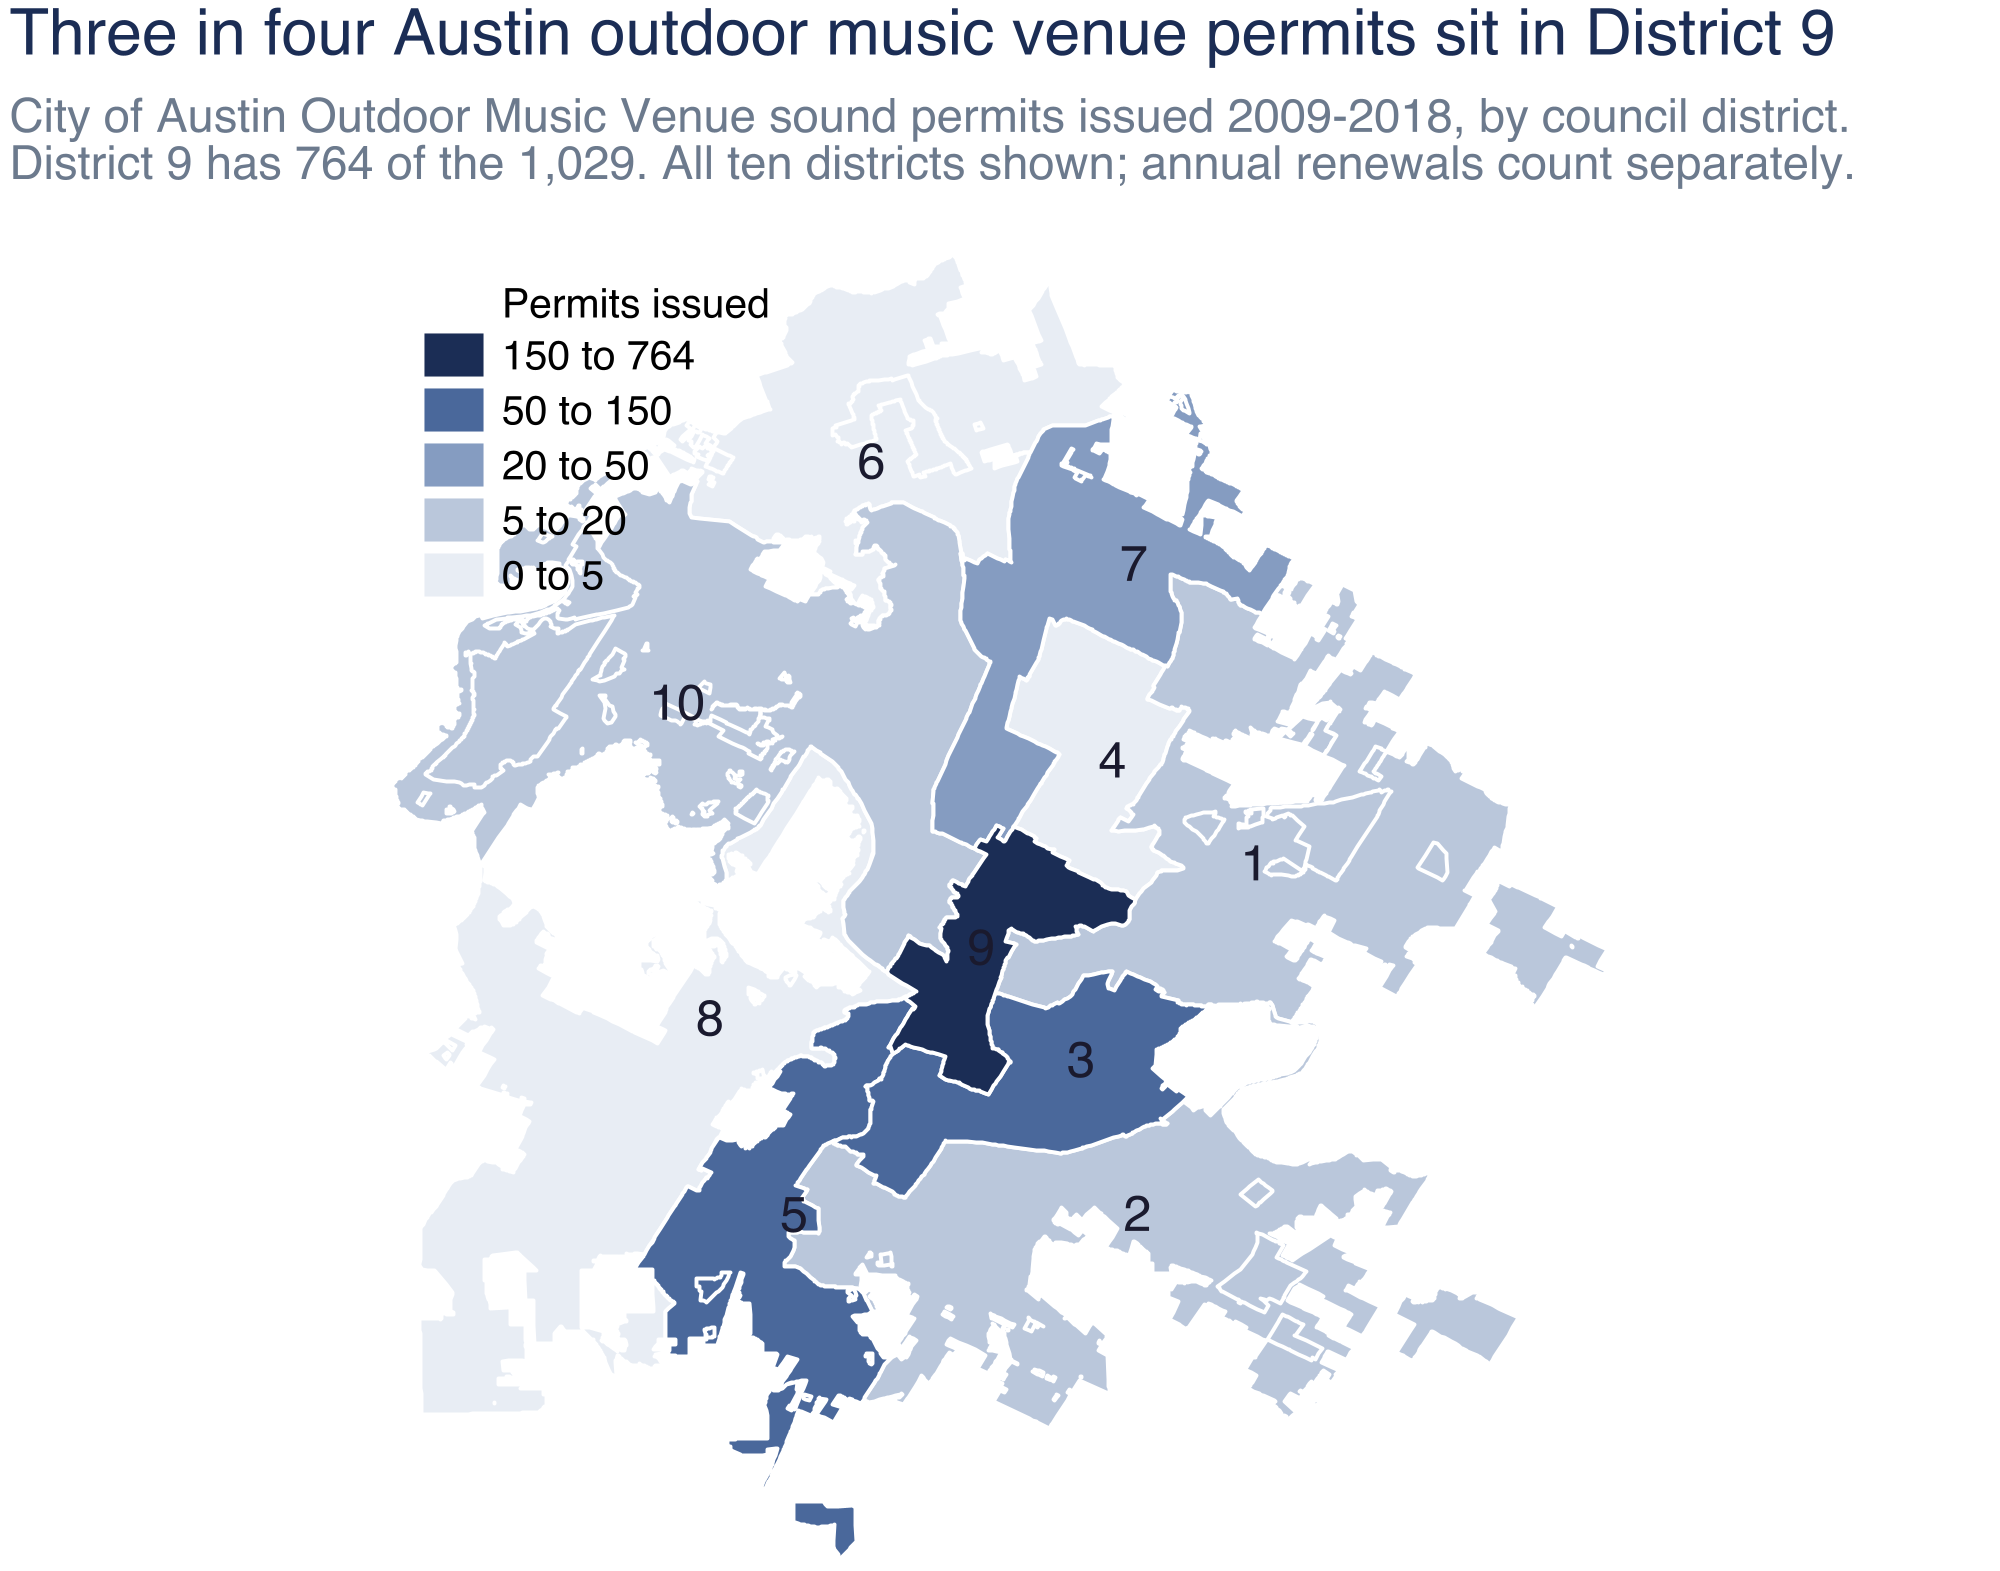
\includegraphics[width=0.82\textwidth]{fig10b_district_map.png}
\caption{Outdoor Music Venue sound permits issued by the City of Austin,
2009--2018, by council district. Source: City of Austin, \textit{Sound
Ordinance Permits, geographic extract}, Socrata dataset \texttt{g3rj-dfgm} at
\url{https://data.austintexas.gov/resource/g3rj-dfgm.csv}, retrieved 1 August
2026; council district boundaries from City of Austin open data. How to read
it: darker districts issued more permits, and the class breaks are set by hand
because the permit distribution is too concentrated in District 9 for equal
intervals to separate anything. Caveats: annual renewals count as separate
permits, so one room can appear many times and the map shows permitted
activity, not distinct rooms; permits are assigned to the council district
boundaries now in force, which took effect in January 2015, so the 2009-to-2014
permits are mapped retrospectively onto districts that did not exist when they
were issued; and the series stops at 2018 because the geocoded file contains
only a partial extract for 2019 (13 rows against the 99 the City by-year count
reports).}
\label{fig:districtmap}
\end{figure}

Between 2009 and 2018, permitted outdoor music activity concentrated in
Council District 9, which covers downtown Austin and the central corridors,
and District 9 accounted for \NVenueOmvPermitsDistrictNineShare\ of the
\NVenueOmvPermitsGeoTwoZeroZeroNineTwoZeroOneEight\ Outdoor Music Venue permits
the City issued in those years. Citywide, the Music \& Entertainment Division's
Outdoor Music Venue permits have since fallen \NVenueOmvPctFromPeak\ from
their 2014--2017 peak, so the geography of permitted outdoor music activity may
have moved since 2018. The curated receipts panel cannot test that
distributional question independently, because its own coverage skews central
by construction.

A separate news-derived timeline of \NVenueClosuresDatedN\ Austin
live-music venue closures reported between January 2015 and June 2026, coded
by primary reason, puts property pressure level with the pandemic:
\NVenueClosuresCovid\ closures cite COVID and
\NVenueClosuresProperty\ cite a property cause, meaning a rent increase, a
sale of the building, a lease expiry or redevelopment.\footnote{The timeline
lists \NVenueClosuresDatedN\ Austin live-music venue closures dated between
January 2015 and June 2026, coded by primary reason from local news coverage
in \emph{Austin Chronicle}, \emph{Austin American-Statesman}, KUT/KUTX,
\emph{Austin Monitor} and CultureMap Austin, plus follow-up items from
\emph{Do512} and \emph{Texas Monthly}, compiled for this study and released
as the project evidence file
\texttt{01\_evidence/08\_venues\_ecosystem/venue\_timeline.csv}. Reasons are
journalist-cited rather than audited, only the primary reason is coded when a
venue reports more than one, and \NVenueClosuresNoReason\ closures have no
reason stated in the sources examined. The timeline is a news-derived record
rather than a register, so it misses venues the research team did not find
coverage for, and an absence here means not found rather than nothing happened.
A separate cross-check against the Comptroller mixed-beverage file found
\NVenueClosureCrossvalContinue\ venues still filing receipts after their
reported closure date, which usually means the programming ended before the
business did.} Respondents to the 2022 Greater Austin Music Census who present
live music, most of whom are not primary venue operators, ranked property tax
first among the nine business pressures the census asked them to rank
(Section~\ref{sec:census}). The two records both point at the cost and security
of the building, though they measure different things: a tax on owners in the
census answer, and rent, sale and tenure in the news timeline.

\subsection{Three tests find no detectable change in the receipts}

Each test below compares the panel venues exposed to a particular intervention
against the rest of the mixed-beverage panel. The panel is the natural setting
for these tests because each intervention hit a small, named set of Austin
live-music rooms and left a monthly, room-level receipts trail on either side
of the event, which is exactly what a before-and-after comparison against a
non-treated group needs.

\textbf{The 2017 extended-hours pilot.} Five named Red River venues ran later
outdoor music hours in 2017 under a City of Austin sound-ordinance pilot; the
only ordinance text located names the pilot as a six-month experiment later
extended to 30 April 2018.\footnote{City of Austin, Law Department, \textit{Draft
ordinance amending City Code Chapter 9-2 (Red River extended-hours pilot)},
dated 30 March 2018, at
\url{https://services.austintexas.gov/edims/document.cfm?id=296553}, retrieved
1 August 2026. The City evaluation memo referenced in the press has not been
located, so the pilot window used in the reported city evaluation (May to
November 2017) and the window the Law Department draft ordinance describes do
not match; both are reported below.} Press accounts of a City evaluation
reported a \NQuasiRedriverClaimUnverified\ rise in payments to local musicians,
alongside 10 percent more local and regional acts booked and 13 percent fewer
total tickets sold; the evaluation memo behind those figures has never been
located and nobody has independently checked them. The Comptroller receipts
contain no matching change in venue revenue.
Once venue-specific seasonality is absorbed, which matters because six of the
pilot window's seven months fall in the second half of the year, the estimate
is \NQuasiRedriverDidSeasonadj\ log points. The unadjusted specification gives
\NQuasiRedriverDidCoef\ log points but fails its own pre-trend test.
Randomization inference on the unadjusted specification, which asks how large
an estimate the same regression produces when five other panel venues are
labelled as treated at random, gives an exact $p =$
\NQuasiRedriverRiP\ across 5,000 placebo draws.\footnote{The specification is
\(\ln R^{\mathrm{real}}_{it} = \alpha_i + \tau_t
   + \beta\,(\mathrm{Pilot}_i \times W_t) + \varepsilon_{it}\),
where \(\mathrm{Pilot}_i\) is one for the five named venues, \(W_t\) is one
for the months of the reported pilot window from May to November 2017, and
\(\alpha_i\) and \(\tau_t\) are venue and year-month fixed effects. The sample
is the panel venues from January 2015 to December 2019 with the large ticketed
rooms excluded. With five treated venues a cluster-robust standard error is
not trustworthy, so inference is by randomization instead: the treatment dates
are held fixed, five venues are drawn at random without replacement from the
panel venues filing in nearly every month of the window, the same regression is
refitted on the placebo assignment, and the exact p-value is
\[
p = \frac{1 + \#\{\,r \le R : |\hat\beta_r| \ge |\hat\beta|\,\}}{R + 1},
\]
where \(\hat\beta\) is the estimate under the assignment that actually
happened, \(\hat\beta_r\) is the estimate under placebo assignment \(r\), and
\(R\) is 5,000, the number of draws. Adding one to numerator and denominator
counts the observed assignment among the possibilities, which is what keeps
the test exact rather than approximate. The bound quoted next comes from that
same placebo distribution: 90 percent of placebo estimates fall inside roughly
plus or minus 14 percent, so an effect larger than that would have shown. The
five venues were named into the pilot rather than drawn into it, so this is
descriptive.} Nine in ten placebo assignments produce estimates inside roughly
plus or minus 14 percent, so a receipts effect much larger than that would
probably have been visible here.\footnote{Pre-trends fail as first specified (p =
\NQuasiRedriverPretrendP), but the cause is seasonality rather than divergence:
the pilot window was six-sevenths second-half months. The pre-trend check
replaces the single interaction with half-year terms,
\(\ln R^{\mathrm{real}}_{it} = \alpha_i + \tau_t
   + \sum_{h \neq h_0} \pi_h\,(\mathbf{1}\{\mathrm{halfyear}(t) = h\}
   \times \mathrm{Pilot}_i) + \varepsilon_{it}\),
with the second half of 2016 as the omitted base \(h_0\), and tests jointly
whether the three half-years before the pilot are all zero,
\(H_0: \pi_{2015\mathrm{H}1} = \pi_{2015\mathrm{H}2}
   = \pi_{2016\mathrm{H}1} = 0\),
by a Wald test with standard errors clustered by venue. Absorbing
venue-specific seasonality, by adding a venue-by-month-of-year fixed effect
that lets each room have its own December and its own March rather than only
the seasonality the whole market shares, clears the pre-trend (p =
\NQuasiRedriverPretrendPSeasonadj) and moves the estimate to
\NQuasiRedriverDidSeasonadj. The reported May-to-November
window also conflicts with the only ordinance text in hand, which describes a
six-month pilot later extended to 30 April 2018.} \textbf{This does not disprove
the \NQuasiRedriverClaimUnverified\ claim.} Mixed-beverage receipts measure
alcohol sales, not the
door split between venue and performer, so a venue could raise what it pays
performers by a fifth without changing its bar takings.

\textbf{The 2024 Live Music Fund venue grants.} The City of Austin
awarded \NQuasiLmfTwoFourVenueAwards\ Live Music Fund venue grants in fiscal
2024, all at the same dollar amount.\footnote{City of Austin, \textit{Austin
Live Music Fund, FY2024 Awardee List}, at
\url{https://austin.widen.net/content/bpzuacfkk8/pdf/FY24-AwardeeList_Austin-Live-Music-Fund.pdf},
retrieved 1 August 2026. All \NQuasiLmfTwoFourVenueAwards\ awards were made at
\$60,000. The full FY2024 award total, adding musician and non-venue promoter
awardees, is 136 awards / \$4,365,000 by independent line-item tally. Program
mechanics and the fund's revenue source are the subject of
Section~\ref{sec:city}.} Against other tracked panel venues the estimate is
\NQuasiLmfTwoFourPostCoef\ log points, about 9 percent, with an exact
randomization-inference $p =$ \NQuasiLmfTwoFourRiP\ across 2,000 placebo draws.
No divergence between grantees and non-grantees is detectable in the years
before the awards ($p =$ \NQuasiLmfTwoFourPretrendP), though that window spans
the pandemic and the parallel-paths test has little power with 15 treated
venues; restricted to 2018 and 2019, the same joint test gives $p =$
\NQuasiLmfTwoFourPretrendPPrepandemic.\footnote{The specification is
\(\ln R^{\mathrm{real}}_{it} = \alpha_i + \tau_t
   + \beta\,(\mathrm{Grant}_i \times \mathrm{Post2024}_t) + \varepsilon_{it}\),
where \(\mathrm{Grant}_i\) is one for a fiscal 2024 venue grantee and
\(\mathrm{Post2024}_t\) is one from January 2024 onward, on monthly
observations from January 2018 to December 2025 with the large ticketed rooms
excluded and standard errors clustered by venue. Grantees with too few filings
in the base year to have a pre-period, and the one large room among them,
leave the estimation sample, so the regression rests on fewer venues than
received awards. The parallel-paths check is an annual event study with 2023
as the omitted base and a joint Wald test that the pre-award year terms are
all zero, \(H_0: \beta_{2018} = \beta_{2019} = \beta_{2020} = \beta_{2021} =
\beta_{2022} = 0\); that window spans the pandemic, so it asks whether the two
groups followed the same path through it; the narrower 2018-and-2019 version
quoted in the text rests on the 12 of 15 grantee venues already filing in 2019.
Randomization inference draws
the same number of placebo grantees from the venues meeting the same
filing-coverage requirement and computes the exact p-value by the formula
above, over 2,000 draws.} Grants are competitively scored, so recipients
differ from non-recipients in whatever the scoring rewarded, and the estimate is
an association rather than a program effect. The
\NQuasiLmfFyTwoSixNotEvaluable\ of the fiscal 2026 round cannot
be tested at all: the city made those awards in March 2026 and the receipts
panel ends that June.

\textbf{The Moody Center.} The Moody Center, a 15,000-seat multipurpose arena
on the University of Texas at Austin campus, opened for public events in April
2022.\footnote{Moody Center, \textit{About}, at
\url{https://www.moodycenteratx.com/about}, retrieved 1 August 2026; opening
event reported in local news coverage the same month. The arena competes for
concert bookings at the top of the market rather than at the size of the
tracked live-music rooms, so any spillover to the venue panel would appear as
a proximity gradient in receipts, not as a shift in the market average.} The
test asks whether panel venues near the arena traded differently from panel
venues farther out after it opened. Within four miles of the arena the
post-opening pattern does not vary with distance ($p =$
\NQuasiMoodyJointP). The design cannot say more than that: the comparison
group is only six venues more than four miles out, every distance-band standard
error is large, and no band is individually distinguishable from zero.\footnote{All three bands enter one regression,
\[
\ln R^{\mathrm{real}}_{it}
  = \alpha_i + \tau_t
  + \sum_{b=1}^{3} \beta_b\,
    \bigl(\mathrm{Band}_{bi} \times \mathrm{Post}_t\bigr)
  + \varepsilon_{it},
\]
where \(\mathrm{Band}_{bi}\) is one when venue \(i\) sits under one mile, one
to two miles, or two to four miles from the arena, venues more than four miles
away are the omitted reference group, and \(\mathrm{Post}_t\) is one from
April 2022 onward. Distance is straight-line miles from the arena's
coordinates, computed by the great-circle formula
\(D = 2\rho\arcsin\sqrt{\sin^{2}(\Delta\phi/2)
   + \cos\phi_1\cos\phi_2\sin^{2}(\Delta\lambda/2)}\),
with \(\phi\) latitude, \(\lambda\) longitude, and \(\rho\) the Earth's radius
in miles. The pre-period is January 2018 to December 2019 and the post-period
July 2022 to December 2025, so neither period includes the pandemic. The quoted
p-value is a Wald test of \(H_0: \beta_1 = \beta_2 = \beta_3\), which asks
whether the post-opening pattern varies with distance at all rather than
whether any single band moved; a continuous version replacing the bands with
post-opening times log distance is registered separately, so nothing rests on
where the band cuts fall. Standard errors are clustered by venue. Distance is
not assigned at random: near venues are central-city rooms and differ from
suburban ones in many ways at once, so this is a description of where the
divergence sits. Note also that any market-wide arena effect is absorbed by the
year-month fixed effects by construction, so this design tests proximity and not
the arena's overall effect on venue receipts.}

These receipts describe what rooms sold at the register. They do not describe
who played in them. Section~\ref{sec:census} turns to the only current
Austin-specific measurement of the people who work in those rooms, the 2022
Greater Austin Music Census, and takes up the retention question the receipts
panel cannot answer. Federal pandemic relief, the one intervention with a
visible signature in the mixed-beverage receipts, waits until
Section~\ref{sec:state}, because that signature traces the eligibility rule
rather than the program's effect and belongs with the state and national
programs.

% Section on the 2022 music census microdata. This is the only current
% Austin-specific measurement of this workforce, and its retention finding is
% the report's most novel result.
\section{What musicians say about staying}
\label{sec:census}

Section~\ref{sec:venues} counted rooms. The only current Austin-specific
measurement of the people who play in those rooms is the 2022 Greater Austin
Music Census, an online instrument that Sound Music Cities fielded with the
City of Austin Music \& Entertainment Division between 15 July and 12 September
2022.\footnote{Sound Music Cities is the consultancy that has run the same
instrument across a rolling cohort of U.S.\ cities since 2022 (Sacramento,
Nashville, New Orleans, Washington D.C., Minneapolis, Cleveland, Baltimore,
and others; the full roster is listed in the references). The Austin fielding
was distributed through community mailing lists, the city's Music \&
Entertainment Division channels, and partner organizations. The city
publishes the individual respondent records as an open dataset,
\textit{2022 Austin Music Census: Details}, Socrata identifier
\texttt{an3p-3yqx}, at \url{https://data.austintexas.gov/resource/an3p-3yqx.csv},
retrieved 1~August 2026. The three Sound Music Cities reports that accompany
the microdata (\textit{Summary Report}, \textit{Data Appendix}, and
\textit{DEI Data Appendix}) are the source for anything printed above the
respondent level; the underlying \NCensusNRespondents\ records are the source
for this study. The Summary Report headline count is 2,260; the microdata
release carries 33 fewer rows and the release documents no reason. Every share
in this section uses the \NCensusNRespondents-row microdata file, so a value
here can sit a few tenths of a point away from a published percentage even
where the two agree.} The 2022 instrument dropped the dollar-denominated income
questions the 2014 fielding had asked, so it cannot say what a musician earns,
but it kept a great deal else: work volume, workspace, tenure, insurance,
business spending, three-year intent, and a ranked list of business
pressures.\footnote{The 2014 census, run by the same authoring team on behalf
of the city, asked for calendar-year 2013 music income in banded form. The
2022 authors state that they dropped the item to raise completion rates and
because respondents had told them the frame did not fit self-employed and
mixed-income careers; see \textit{Summary Report}, printed p.~6, at
\url{https://www.austinmusiccensus.org/}. The consequence is that Austin's own
music census has not asked what a musician earns for the twelve years running.}
This study reads the census from the respondent-level file rather than the
published tables, because a per-respondent construction is needed for two
questions the printed report cannot answer: whether one person's two three-year
answers move together, and whether the widely cited spending headline describes
any actual person.

That file records \NCensusNRespondents\ respondents across 107 variables. Every
number in this section describes those respondents and not the Austin music
workforce.\footnote{The census was a self-selected online instrument with no
design or post-stratification weights. It is not a probability sample of
Austin's music workforce, and a probability-sample benchmark for the same
population does not exist. Every share in this section is therefore a
descriptive statistic on the people who answered, not a population estimate,
and none is comparable with the American Community Survey estimates in
Section~\ref{sec:earnings}, the Bureau of Labor Statistics wage series in
Section~\ref{sec:payroll}, or the Comptroller receipts panel in
Section~\ref{sec:venues}. No standard error or margin of error is computed
anywhere in this section. Item nonresponse is heavy and uneven, and several
blocks were routed only to performers or only to venue operators, so every
statistic in this section is reported against its own denominator. Six
figures computed here reproduce the Sound Music Cities \textit{Data Appendix}
to within a percentage point (the two three-year retention shares, the mean
and median distance travelled to work, the sum-of-means spending headline, and
the local share of spending), which is the best available check that the file
is being read correctly.}

\subsection{Most respondents expect to stay in music; far fewer expect to stay in Austin}

The same \NCensusRetentionDenom\ respondents answered both three-year questions,
so the comparison below is between one person's two answers rather than between
two groups. \NCensusIntendContinueMusic\ answered definitely or maybe yes to
still working in music, and \NCensusIntendStayAustin\ answered definitely or
maybe yes to still living in greater Austin, a within-person gap of
\NCensusRetentionGap.\footnote{Each share is an unweighted count over its own
denominator, \(\hat p = 100 \times n_{\mathrm{yes}}/n_{\mathrm{answered}}\),
where \(n_{\mathrm{yes}}\) counts respondents answering definitely or maybe yes
and \(n_{\mathrm{answered}}\) counts everyone who answered that item. A
respondent who skipped the item is out of both numerator and denominator
rather than counted as a no. The retention gap is the difference of the two
shares on the same respondents,
\(\hat p_{\mathrm{music}} - \hat p_{\mathrm{Austin}}\), which is a within-person
comparison and not a comparison of two groups. No weight enters anywhere in
this section, because the release carries none, so no margin of error can be
computed. Both retention shares reproduce the Sound Music Cities
\textit{Summary Report} p.~7 to the tenth of a percentage point on the
microdata file.} Most of the complement to the Austin share is uncertainty
rather than stated departure: among the \NCensusRetentionDenom\ respondents,
about a quarter answered ``unsure'' and roughly one in ten answered maybe or
definitely no, which is a weaker claim than a third planning to
leave.\footnote{The Austin item's five options are definitely yes, maybe yes,
unsure, maybe no, and definitely no. The full breakdown on the
\NCensusRetentionDenom\ respondents is 44.2\% definitely yes, 19.9\% maybe
yes, 25.6\% unsure, 6.7\% maybe no, and 3.6\% definitely no; the two shares
combined into ``definitely or maybe yes'' produce \NCensusIntendStayAustin.
Read the 25.6\% unsure share as respondents who could not answer, not as
respondents who leaned toward leaving.}

\begin{figure}[htbp]
\centering
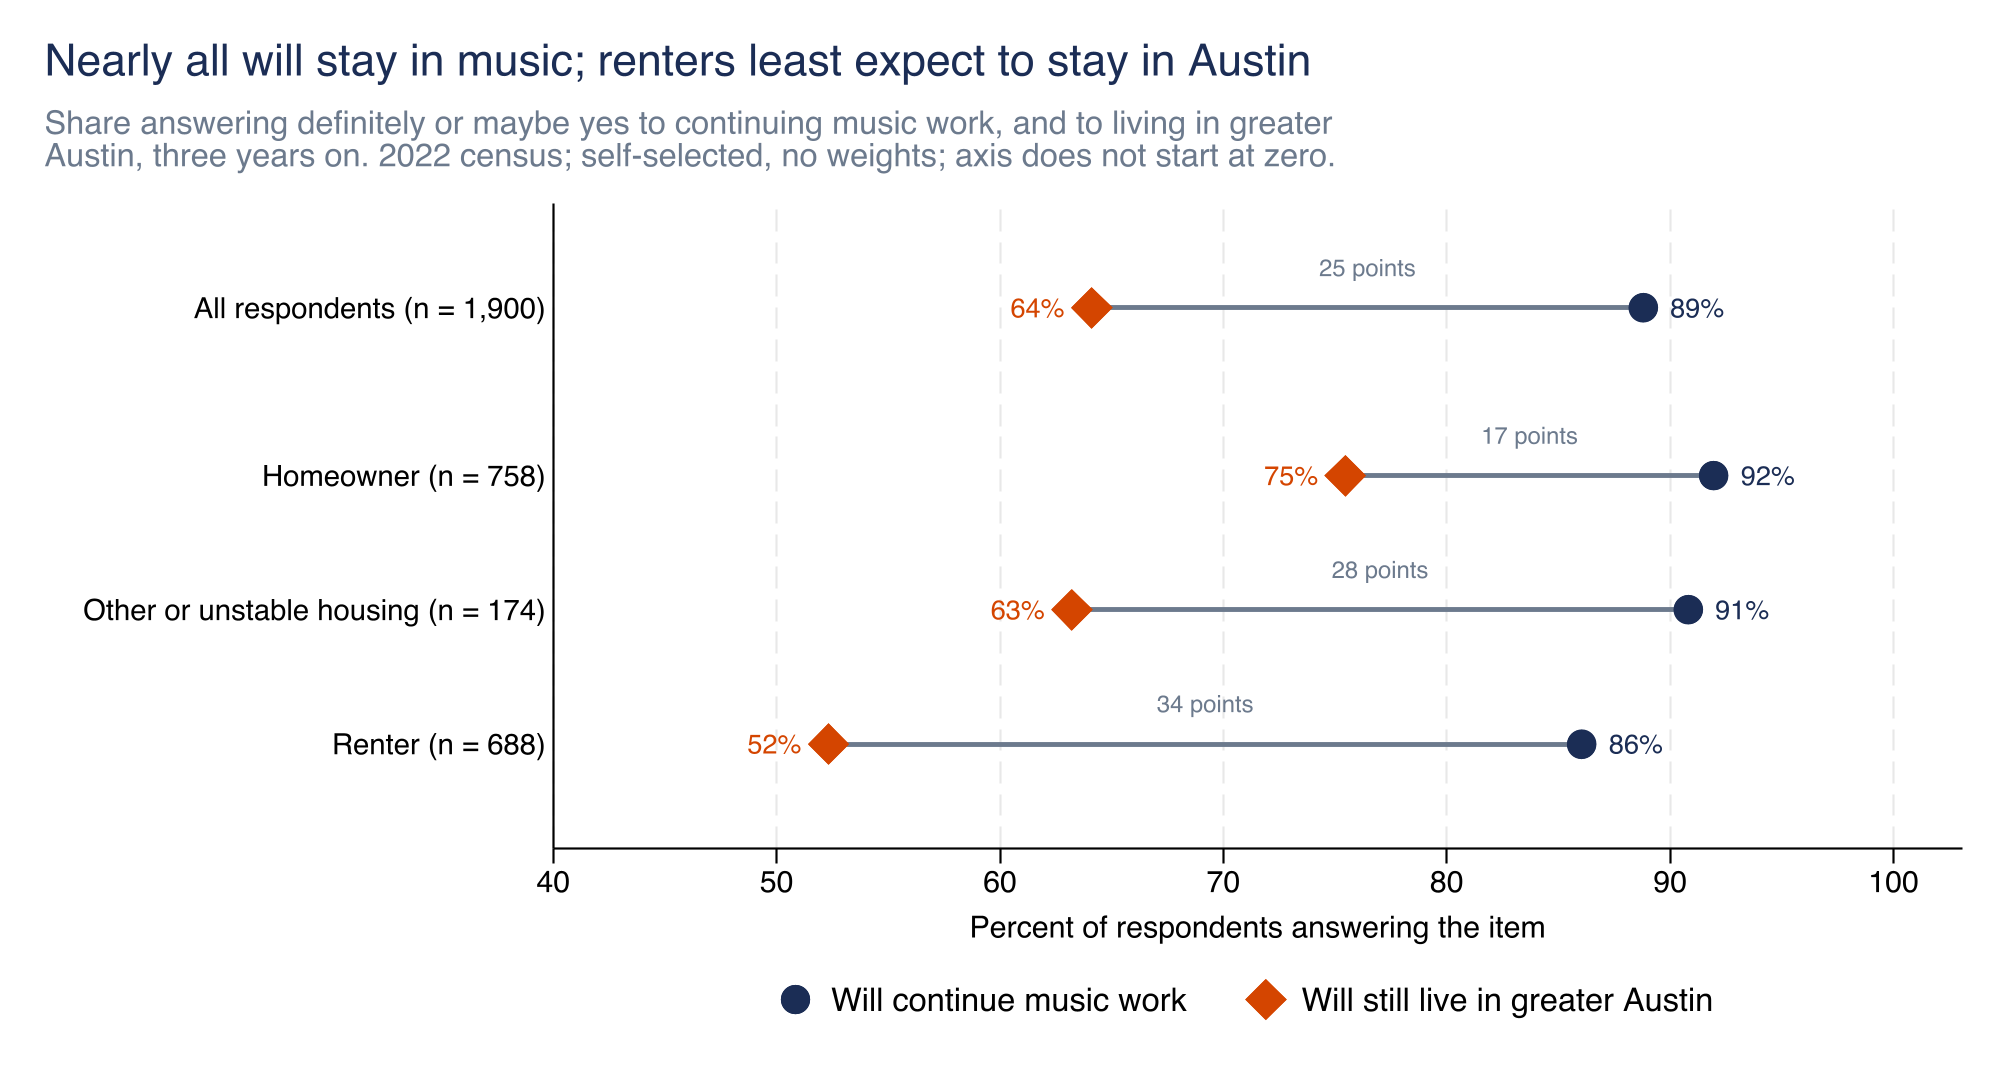
\includegraphics[width=\textwidth]{fig26_retention_split.png}
\caption{Share expecting to continue music work and to remain in greater Austin
three years on, overall and by housing tenure. Source: 2022 Greater Austin
Music Census respondent-level file, Sound Music Cities and City of Austin
Music \& Entertainment Division, City of Austin open data dataset
\texttt{an3p-3yqx}, retrieved 1~August 2026. How to read it: both questions
were answered by the same \NCensusRetentionDenom\ respondents, so the distance
between the two bars is a within-person gap and not a comparison of two
groups. Caveats: this is a self-selected online survey with no weights, so
the percentages describe respondents rather than the Austin music workforce,
and they are not comparable with the American Community Survey estimates in
Section~\ref{sec:earnings}.}
\label{fig:retention}
\end{figure}

\subsection{Housing tenure separates the answers most sharply; sector and workspace do not separate them at all}

Who are the doubtful respondents? Of six respondent characteristics this study
tested against the Austin-retention answer, housing tenure separates it most
sharply: \NCensusStayHousingTenureHomeowner\ of homeowners expected to stay in
greater Austin against \NCensusStayHousingTenureRenter\ of renters, with
\NCensusStayHousingTenureOtherOrUnstableHousing\ of respondents in other or
unstable housing situated between them.\footnote{The homeowner--renter
difference in expected-stay rates is unlikely to be chance among these
respondents: \NCensusStaychiTwoHousingTenure. The test is Pearson's
chi-squared for independence in a two-way table,
\(X^{2} = \sum_{j}\sum_{k}(O_{jk} - E_{jk})^{2}/E_{jk}\) with
\(E_{jk} = R_j C_k / N\), where \(O_{jk}\) is the number of respondents in row
\(j\) and column \(k\), \(R_j\) and \(C_k\) are the row and column totals,
\(N\) is the number answering both items, and \(E_{jk}\) is the count expected
if the two answers were unrelated. The number in parentheses after the
statistic is the degrees of freedom, \((J-1)(K-1)\) for a table with \(J\)
rows and \(K\) columns. In a logistic regression conditioning on primary
music-ecosystem sector, years of experience, and health insurance, renters
have \NCensusLogitRenterOr\ times the odds of expecting to stay in Austin
that homeowners do, on \NCensusLogitN\ respondents who answered every item in
the equation. The specification is
\[
\ln\frac{\Pr(\mathrm{stay}_i = 1)}{1 - \Pr(\mathrm{stay}_i = 1)}
  = \alpha + \sum_s \beta_s\,\mathrm{sector}_{si}
  + \sum_e \gamma_e\,\mathrm{exper}_{ei}
  + \sum_h \delta_h\,\mathrm{tenure}_{hi}
  + \theta\,\mathrm{insured}_i ,
\]
where \(\mathrm{stay}_i\) is one when respondent \(i\) answered definitely or
maybe yes to still living in greater Austin in three years, the
\(\mathrm{sector}_{si}\) are indicators for primary music-ecosystem sector,
the \(\mathrm{exper}_{ei}\) for years-of-experience band, the
\(\mathrm{tenure}_{hi}\) for housing tenure with homeowner omitted, and
\(\mathrm{insured}_i\) is one for holding health insurance. The quantity
quoted is the odds ratio \(e^{\hat\delta_{\mathrm{renter}}}\); a value below
one means renters had lower odds of expecting to stay than homeowners who
match them on sector, experience, and insurance. An odds ratio is not a ratio
of probabilities and sits further from one than the probability ratio does
when the outcome is common, as it is here. Estimation is by maximum
likelihood on the respondents who answered every item in the equation, which
is fewer than answered the retention question alone. Neither the test nor the
regression is weighted, because the census carries no design weights, and
both p-values assume a simple random sample, which a self-selected online
survey is not. Read the test statistics as descriptive discriminants among
respondents rather than as inference to the Austin music workforce.
Tenure was not assigned at random, and income, age, and family stage all
move with it, none of which the census measured; the tenure result is
therefore an association among respondents and not the cost of renting.
The analysis recodes tenure into three mutually exclusive categories, because
the published appendix's categories overlap, which is why the tenure shares
here do not match the \textit{Data Appendix}.} Health insurance separates the
answers the same way: \NCensusStayHealthInsuranceHasHealthInsurance\ of the
1,390 respondents with health insurance expected to stay against
\NCensusStayHealthInsuranceNoHealthInsurance\ of the 254
uninsured.\footnote{The census item is respondent-reported coverage of any
kind (an employer plan, a marketplace plan, Medicaid, Medicare, VA, or
another source), asked as a single yes/no. It is not directly comparable with
the American Community Survey health-insurance coverage rate quoted in the
summary, which uses the ACS multi-item HICOV construction on a probability
sample of households.}

Two music-career characteristics also separate the Austin-retention answer,
though not in a straight line. Years of experience is the second strongest of
the six discriminants (\NCensusStaychiTwoYearsOfExperience), and it runs
non-monotonically across the four experience bands the census reports: the
lowest expected-stay rate belongs to the 6-to-10-year band at
\NCensusStayYearsOfExperienceSixToOneZeroYears, below both newer entrants at
\NCensusStayYearsOfExperienceUnderThreeYears\ (under three years of
experience) and the most experienced at
\NCensusStayYearsOfExperienceMoreThanOneZeroYears\ (more than ten years). How
much of a respondent's music income comes from local gigs also separates the
Austin answer, on the same 1,900 respondents
(\NCensusStaychiTwoMusicIncomeFromLocalGigs).

Two other characteristics do not separate the answers. Neither the
respondent's primary music-ecosystem sector (music creative, music industry,
or venue or presenter) nor the respondent's workspace status (owns, rents,
provided or not needed, or needs but lacks) discriminates the Austin-retention
answer at conventional levels; both are within the range chance would
produce among respondents
(\NCensusStaychiTwoPrimarySector; \NCensusStaychiTwoWorkSpaceStatus).

\begin{keyfinding}
{\small That result ties together two parts of this study.
Section~\ref{sec:costs} showed that Austin's cost problem is centered on
housing more than on prices generally, and this section finds that housing tenure separates the
census respondents' Austin-retention answer more sharply than any of the six
respondent characteristics tested. Health insurance splits the same answer
the same way, so the two strongest household-security measures both
separate stayers from the unsure, while primary sector and workspace access
do not separate them at all.}
\end{keyfinding}

\subsection{Working in music costs money, and the widely cited figure overstates the typical case}

\begin{figure}[htbp]
\centering
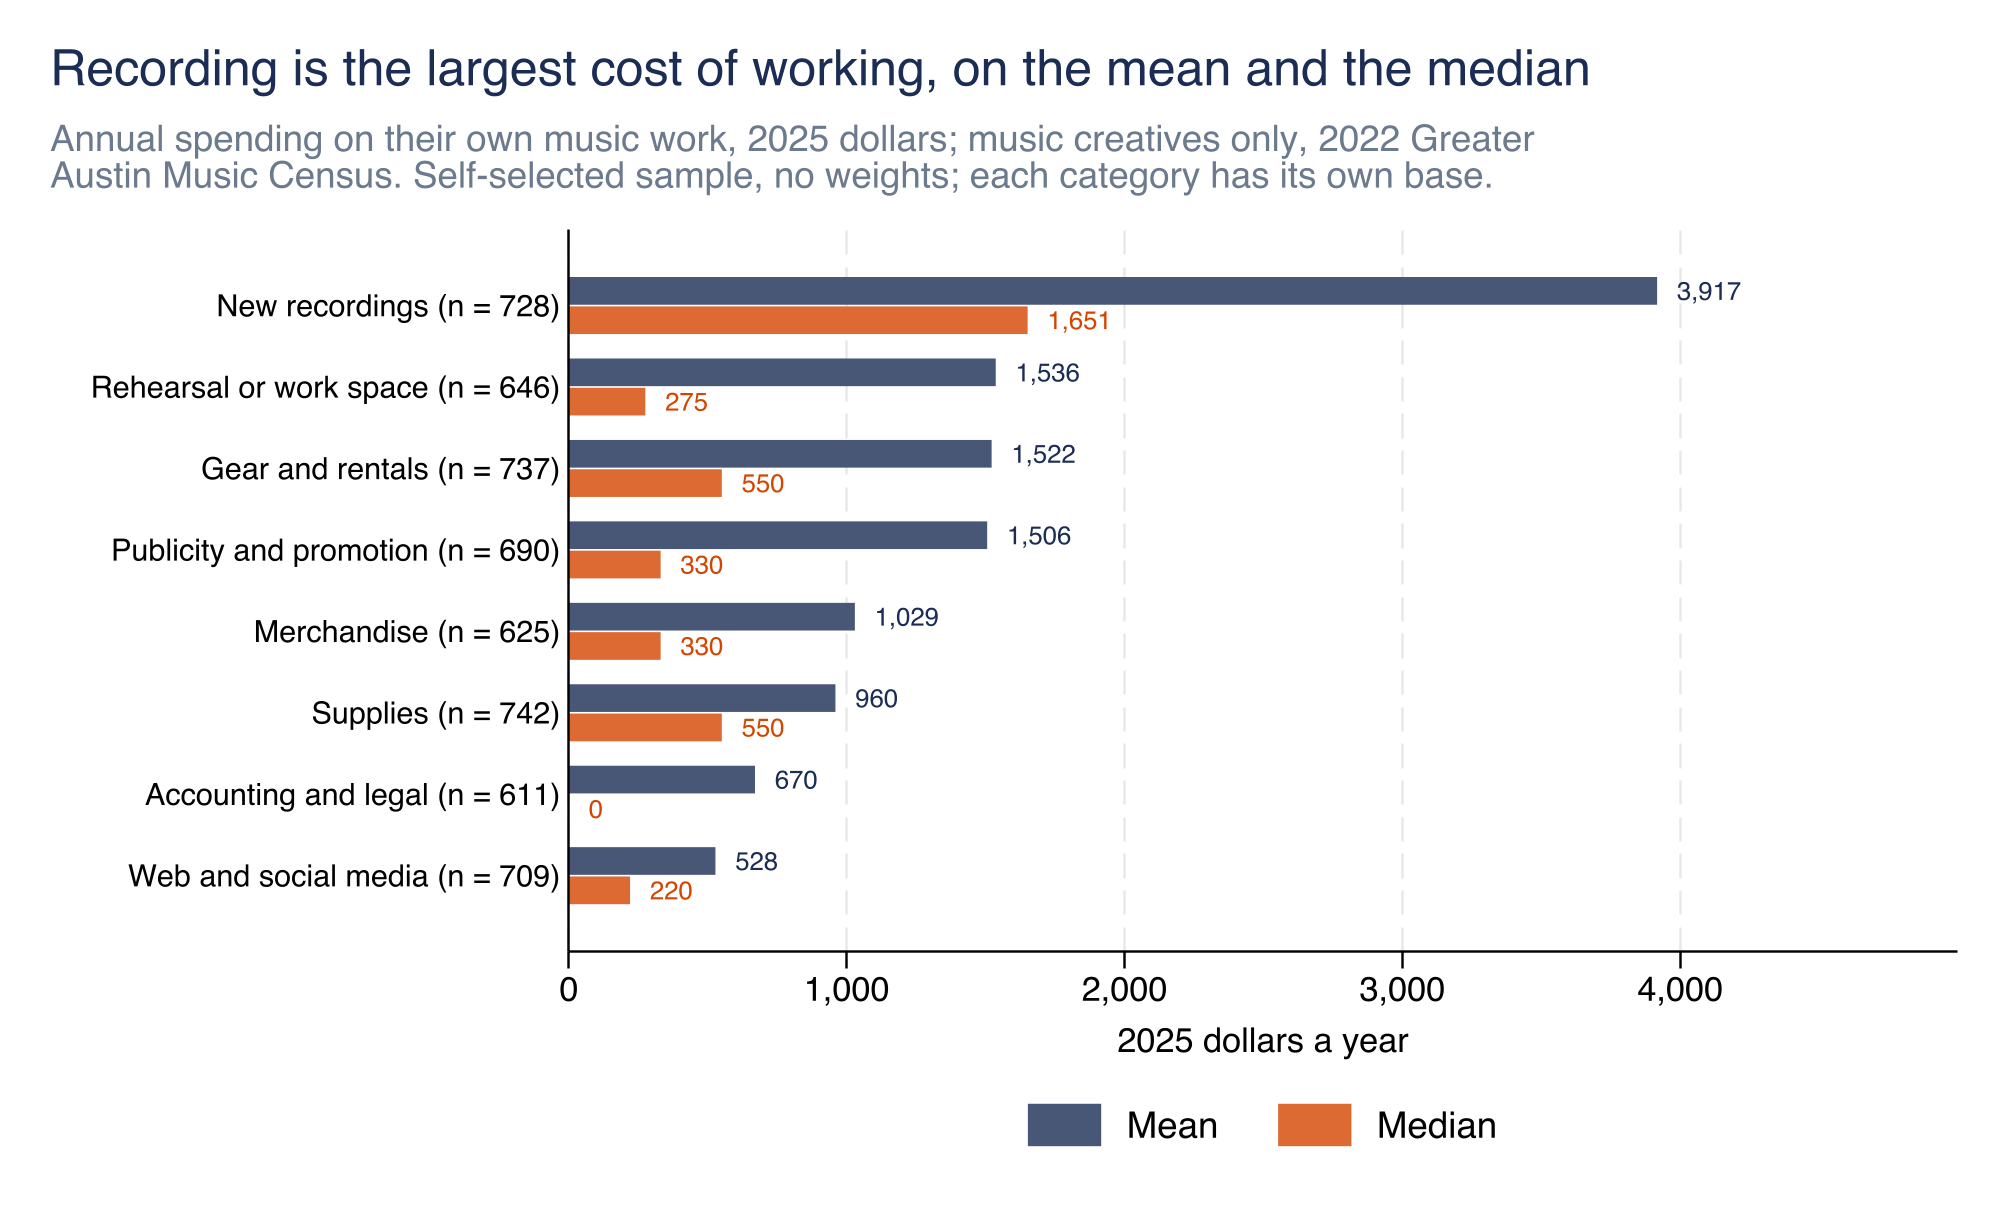
\includegraphics[width=\textwidth]{fig27_cost_of_working.png}
\caption{Annual respondent spending on their own music work, by category,
music creatives only, 2025 dollars. Source: 2022 Greater Austin Music Census
respondent-level file (dataset \texttt{an3p-3yqx}), converted from 2022 to
2025 dollars with the national consumer price index (CPI-U annual factor).
How to read it: mean and median are shown for each category because the
distribution is heavily right-skewed and the median is the better guide to a
typical respondent. Caveats: each category has its own base, ranging from 611
to 742 music creatives; the census is a self-selected online sample and
carries no weights.}
\label{fig:costofworking}
\end{figure}

Coverage of the 2022 census in local media and in the Sound Music Cities
\textit{Data Appendix} often cites an annual music-work spending figure of
about \$10,500 in 2022 dollars, worth \NCensusSpendSumofmeansTwoZeroTwoFive\
in 2025 prices.\footnote{The published \$10,500 headline appears in the Sound
Music Cities \textit{Data Appendix}, printed p.~46. It was widely picked up
locally, including in Austin City Council briefings on the Live Music Fund
and in coverage by KUT News and \textit{Austin Monitor}. The 2022 dollar
inflation factor to 2025 is the ratio of the national CPI-U all-urban annual
averages from the Bureau of Labor Statistics, series identifier
\texttt{CUUR0000SA0}, at \url{https://www.bls.gov/cpi/data.htm}; the same
factor is used throughout this study.} That headline adds together eight
category means computed on eight different sets of respondents, so it does
not describe any actual person. Among the \NCensusSpendCompleteN\ music
creatives who answered every category, the median total is
\NCensusSpendTotalMedian\ and the mean is \NCensusSpendTotalMean, both in
2025 dollars, so the correctly constructed mean sits well below the widely
cited figure and the median sits far below it.\footnote{The widely cited
headline is \(\sum_{k=1}^{8}\bar{x}_k\), where \(\bar{x}_k\) is the mean of
spending category \(k\) taken over \(S_k\), the set of respondents who
answered that category. The eight sets are not the same people. The
per-respondent figures quoted here are built the other way round, summing
within a person first and taking the middle of those totals:
\(\tilde{x} = \operatorname{median}_{i \in S}
   \bigl(\sum_{k=1}^{8} x_{ik}\bigr)\)
over \(S = \bigcap_k S_k\), the respondents who answered every category, so
every dollar in the sum belongs to one person. The two constructions agree
only when each category has the same respondents and the within-person total
is symmetrically distributed, and neither condition holds here. Both are
converted from 2022 to 2025 dollars by \(C_{2025}/C_{2022}\), the ratio of
national CPI-U annual averages, as is the published headline quoted above.
The eight categories in the instrument are gear and rentals, new recordings,
publicity and promotion, merchandise, rehearsal or work space, supplies,
accounting and legal, and travel; the item is asked of music creatives only
and does not appear on the venue-operator branch.} For a single number that
describes a typical respondent, prefer the median: \NCensusSpendTotalMedian\
on the \NCensusSpendCompleteN\ complete-case music creatives, or
\NCensusSpendTotalMedianAnyitem\ on the 873 who answered at least one
category (with unanswered categories treated as zero, a deliberate lower
bound because the release cannot distinguish a true zero from a blank).

These self-reported spending figures cannot be netted against the
Nonemployer Statistics receipts figure quoted in
Section~\ref{sec:payroll}.\footnote{U.S.~Census Bureau, Nonemployer
Statistics, at
\url{https://www.census.gov/programs-surveys/nonemployer-statistics.html}.
Nonemployer Statistics is an administrative-record product built from
business income-tax returns of firms with no paid employees and receipts of
at least \$1{,}000; it reports the receipts side, before expenses, and
carries no expense series. The two numbers therefore cannot be differenced.
They cover different populations (music-industry nonemployer firms in the
Nonemployer file, music creatives in the census), different years, and
different units (businesses in one case and people in the other), and the
census figure is a self-reported cost rather than a tax-return revenue
line.}

\subsection{Respondents who present live music name property tax as their leading pressure}

Among the \NCensusNPresentersRanking\ respondents who both present live music
and completed the nine-item business-pressure ranking,
\NCensusPressureTopThreePropertyTax\ placed property tax in their top three
and \NCensusPressureFirstPropertyTax\ ranked it their single greatest
pressure, ahead of talent costs (\NCensusPressureTopThreeTalentCosts\ in the
top three) and labor cost and retention
(\NCensusPressureTopThreeLaborCostAndRetention).\footnote{The ranking item
asked respondents who present live music, whether as a primary or a
secondary activity, to rank nine business pressures from most to least
pressing. The nine items were building operations and upkeep, changing
audience behavior, labor cost and retention, marketing, neighborhood
redevelopment, ordinances and permitting, property tax, talent costs, and
unpredictable operating costs. \NCensusNPresentersRanking\ respondents
completed the full ranking; that is 8~percent of the \NCensusNRespondents\
respondents in the file and the thinnest block used in this section. This is
a presenter-activity population rather than a venue census: only 77 of the
177 named venue or presenter as their primary sector, and the remaining 100
are music creatives and industry professionals who also present gigs. The
Sound Music Cities \textit{Data Appendix} slides~56--57 split operators from
promoters; the promoter cell falls below this study's 50-record publication
floor and is not reported here.}

That ranking and the closure record in Section~\ref{sec:venues}, where
\NCensusClosuresPropertyShare\ of the 36 dated Austin venue closures cite a
real-estate cause (sale, rent increase, lease expiration, or redevelopment)
against 13 that cite the pandemic, both point at property costs. They do not
point at the same property cost: the census item is a tax that falls on
owners, and the Section~\ref{sec:venues} closure record is dominated by
rent, sale, and lease-tenure disputes at what are mostly tenant venues. The
two sources also diverge in one place. Talent costs rank second among
presenter pressures in the census, but appear as the cause of no closure in
the Section~\ref{sec:venues} record. The Comptroller receipts panel used in
Section~\ref{sec:venues} has no field for what a venue pays performers, so
the talent-cost item is untested here rather than contradicted.

Sections~\ref{sec:city} and \ref{sec:state} turn from what these respondents
report to what the city and the state actually spend on this workforce.

% Section 6: Austin's own money for music. Neutral description of what the
% money did and when, with innocent explanations noted where they exist.
\section{Austin's music money is small, uneven, and has never had a performance audit}
\label{sec:city}

Austin funds music from its Hotel Occupancy Tax, a levy that lodging guests
pay on hotel and short-term-rental stays inside the city. A 2019 ordinance
raised the tax and directed a fixed share of the increase to a Live Music
Fund, so the money moves with hotel demand rather than with any annual
council judgment about musicians.\footnote{City of Austin Ordinance
No.~20190919-149, adopted 19 September 2019 and effective 30 September
2019, raised the Hotel Occupancy Tax rate from 7 to 9 percent and directed
an amount equal to 15 percent of the two-point increase to the Live Music
Fund, another 15 percent to Historic Preservation, and the balance largely
to Convention Center expansion. Because the ordinance fixes the share
rather than reappropriating each year, fund revenue tracks hotel demand.
Ordinance text at
\url{https://services.austintexas.gov/edims/document.cfm?id=328565}.}

\subsection{Live music receives a small share of a large tax}

\begin{figure}[htbp]
\centering
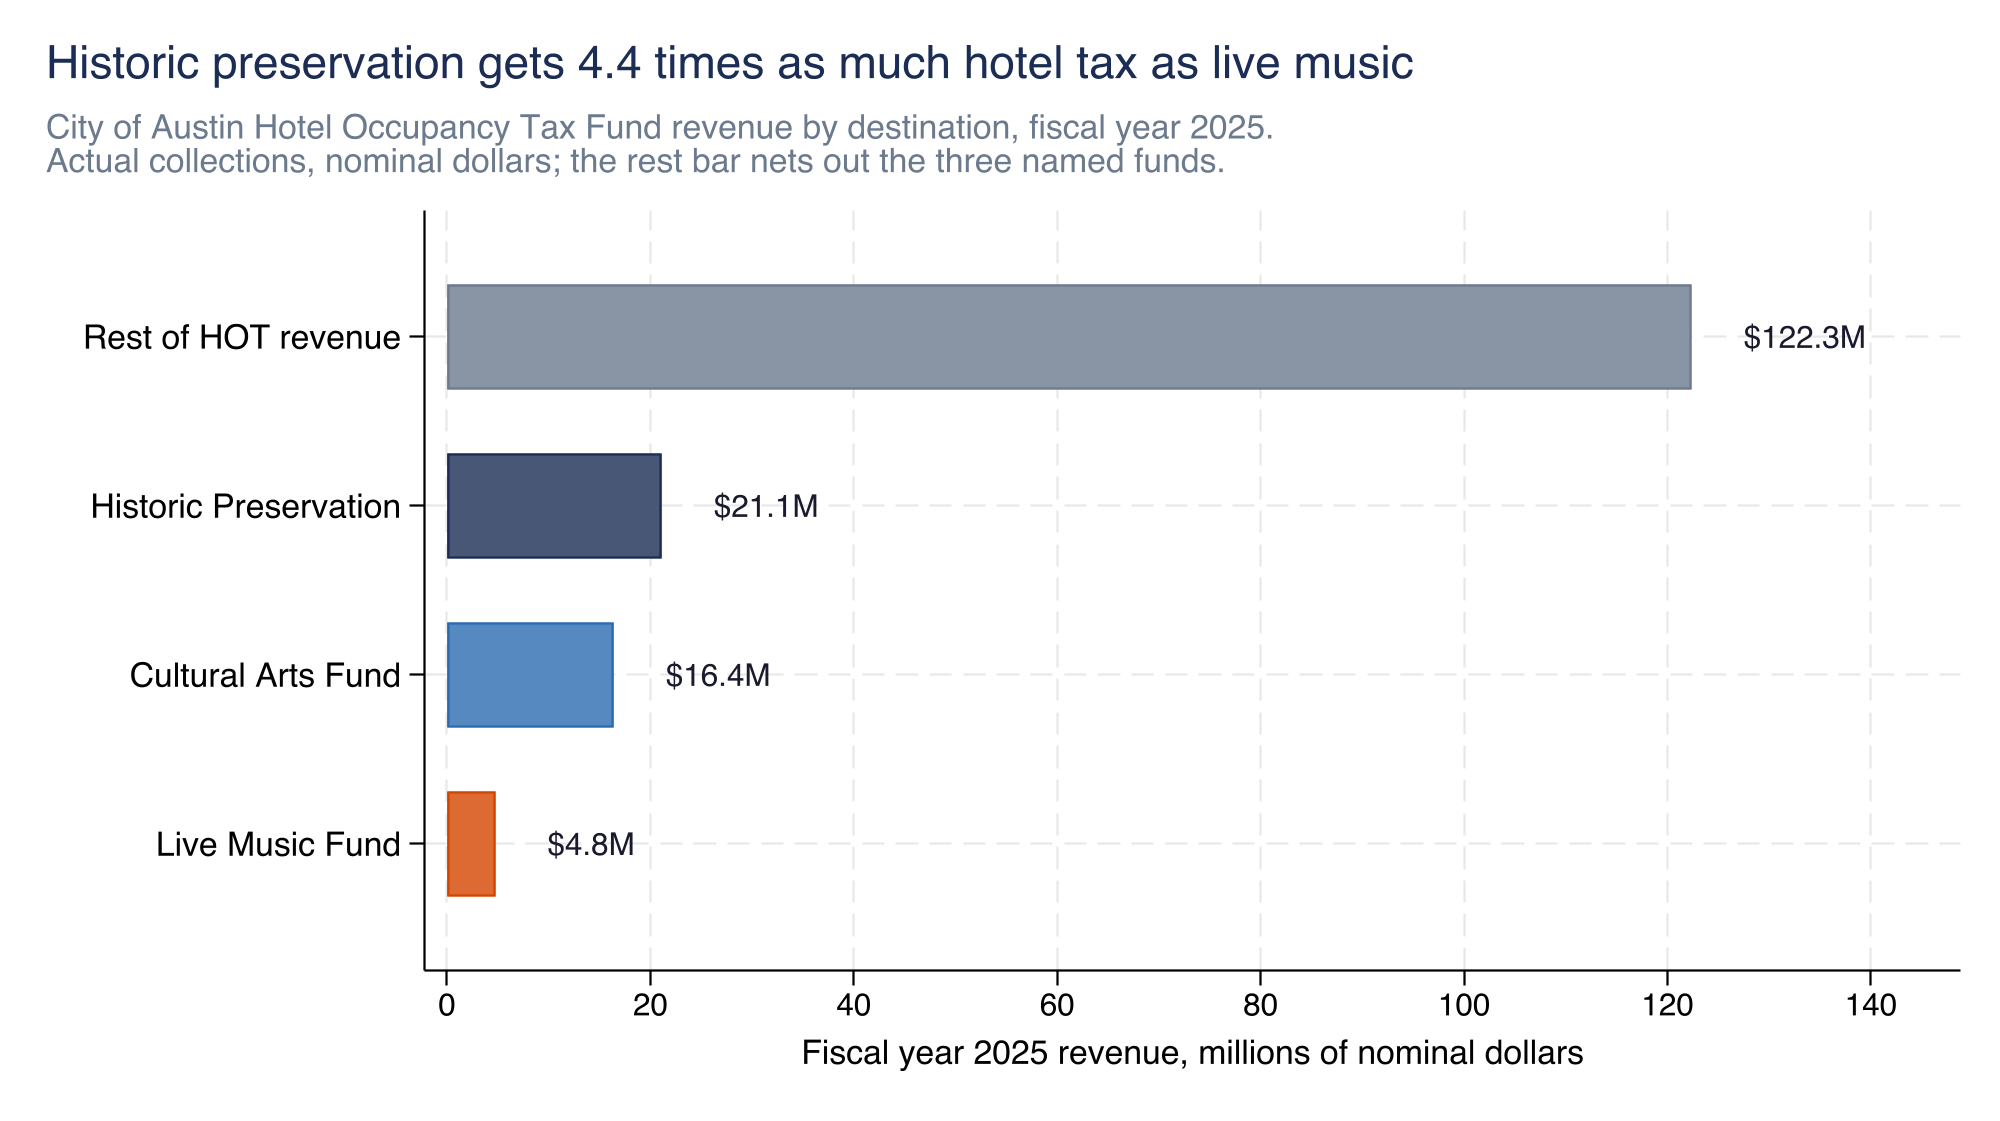
\includegraphics[width=\textwidth]{fig12_hot_allocation.png}
\caption{City of Austin Hotel Occupancy Tax revenue by destination, fiscal
year 2025, nominal dollars. Source: City of Austin Open Budget ATX,
\textit{Revenue Open Budget -- revised} (Socrata dataset 5rhv-xasu),
fund-level actuals for fiscal 2025. How to read it: all bars share one
zero-based axis, so the relative sizes are directly comparable. Caveat: the
residual bar is total hotel-tax revenue minus the three named funds rather
than a single program, and under the 2019 ordinance most of the residual
flows to Convention Center expansion. Because every bar is same-year,
nominal and real dollars give the same picture.}
\label{fig:hotalloc}
\end{figure}

In fiscal 2025 the Live Music Fund received \NCityLmfRevenueFyTwoFive, or
\NCityLmfShareOfHotFyTwoFive\ of the city's
\NCityHotTotalRevenueFyTwoFive\ in Hotel Occupancy Tax
revenue.\footnote{The city's Open Budget ATX portal posts fund-level
actuals for every named city fund by fiscal year; those posted actuals are
the auditable primary record until each year's Annual Comprehensive
Financial Report closes. Fund revenue and Hotel Occupancy Tax totals for
fiscal 2025 in this section come from that portal's \textit{Revenue Open
Budget -- revised} extract, Socrata dataset 5rhv-xasu, retrieved 1 August
2026 from \url{https://data.austintexas.gov/resource/5rhv-xasu.csv}. Same-
year ratios need no deflation because both sides carry the same dollar
base. The Open Budget series begins in fiscal 2021 and does not observe
any earlier fund balance.} The Historic Preservation Fund drew
\NCityHpRevenueFyTwoFive\ from the same tax, \NCityHpToLmfRatioFyTwoFive\
as much as the Live Music Fund. That gap is not a departure from the 2019
ordinance's equal split. The Historic Preservation Fund also receives
hotel-tax money beyond the 15 percent of the two-point increase the
ordinance dedicated to each fund, and on the equal share alone the two
would draw the same amount.

From fiscal 2024 to fiscal 2025, Live Music Fund revenue moved
\NCityLmfRevenuePctchgFyTwoFourFyTwoFiveNominal\ in nominal terms and
\NCityLmfRevenuePctchgFyTwoFourFyTwoFiveReal\ in 2025
dollars.\footnote{Fiscal-year change computed from the same Open Budget
revenue extract as above (dataset 5rhv-xasu). This section approximates
Austin fiscal year \(Y\) by calendar year \(Y\) for deflation, because
Austin fiscal years run October through September and nine of the twelve
months fall in calendar \(Y\); no quarterly deflator was available for the
national consumer price index used here.} That is one year on a series
that tracks hotel demand and has swung widely since 2021, so it should not
be read as a trend.

\subsection{The fund collected for two observed years before it paid musicians}

\begin{figure}[htbp]
\centering
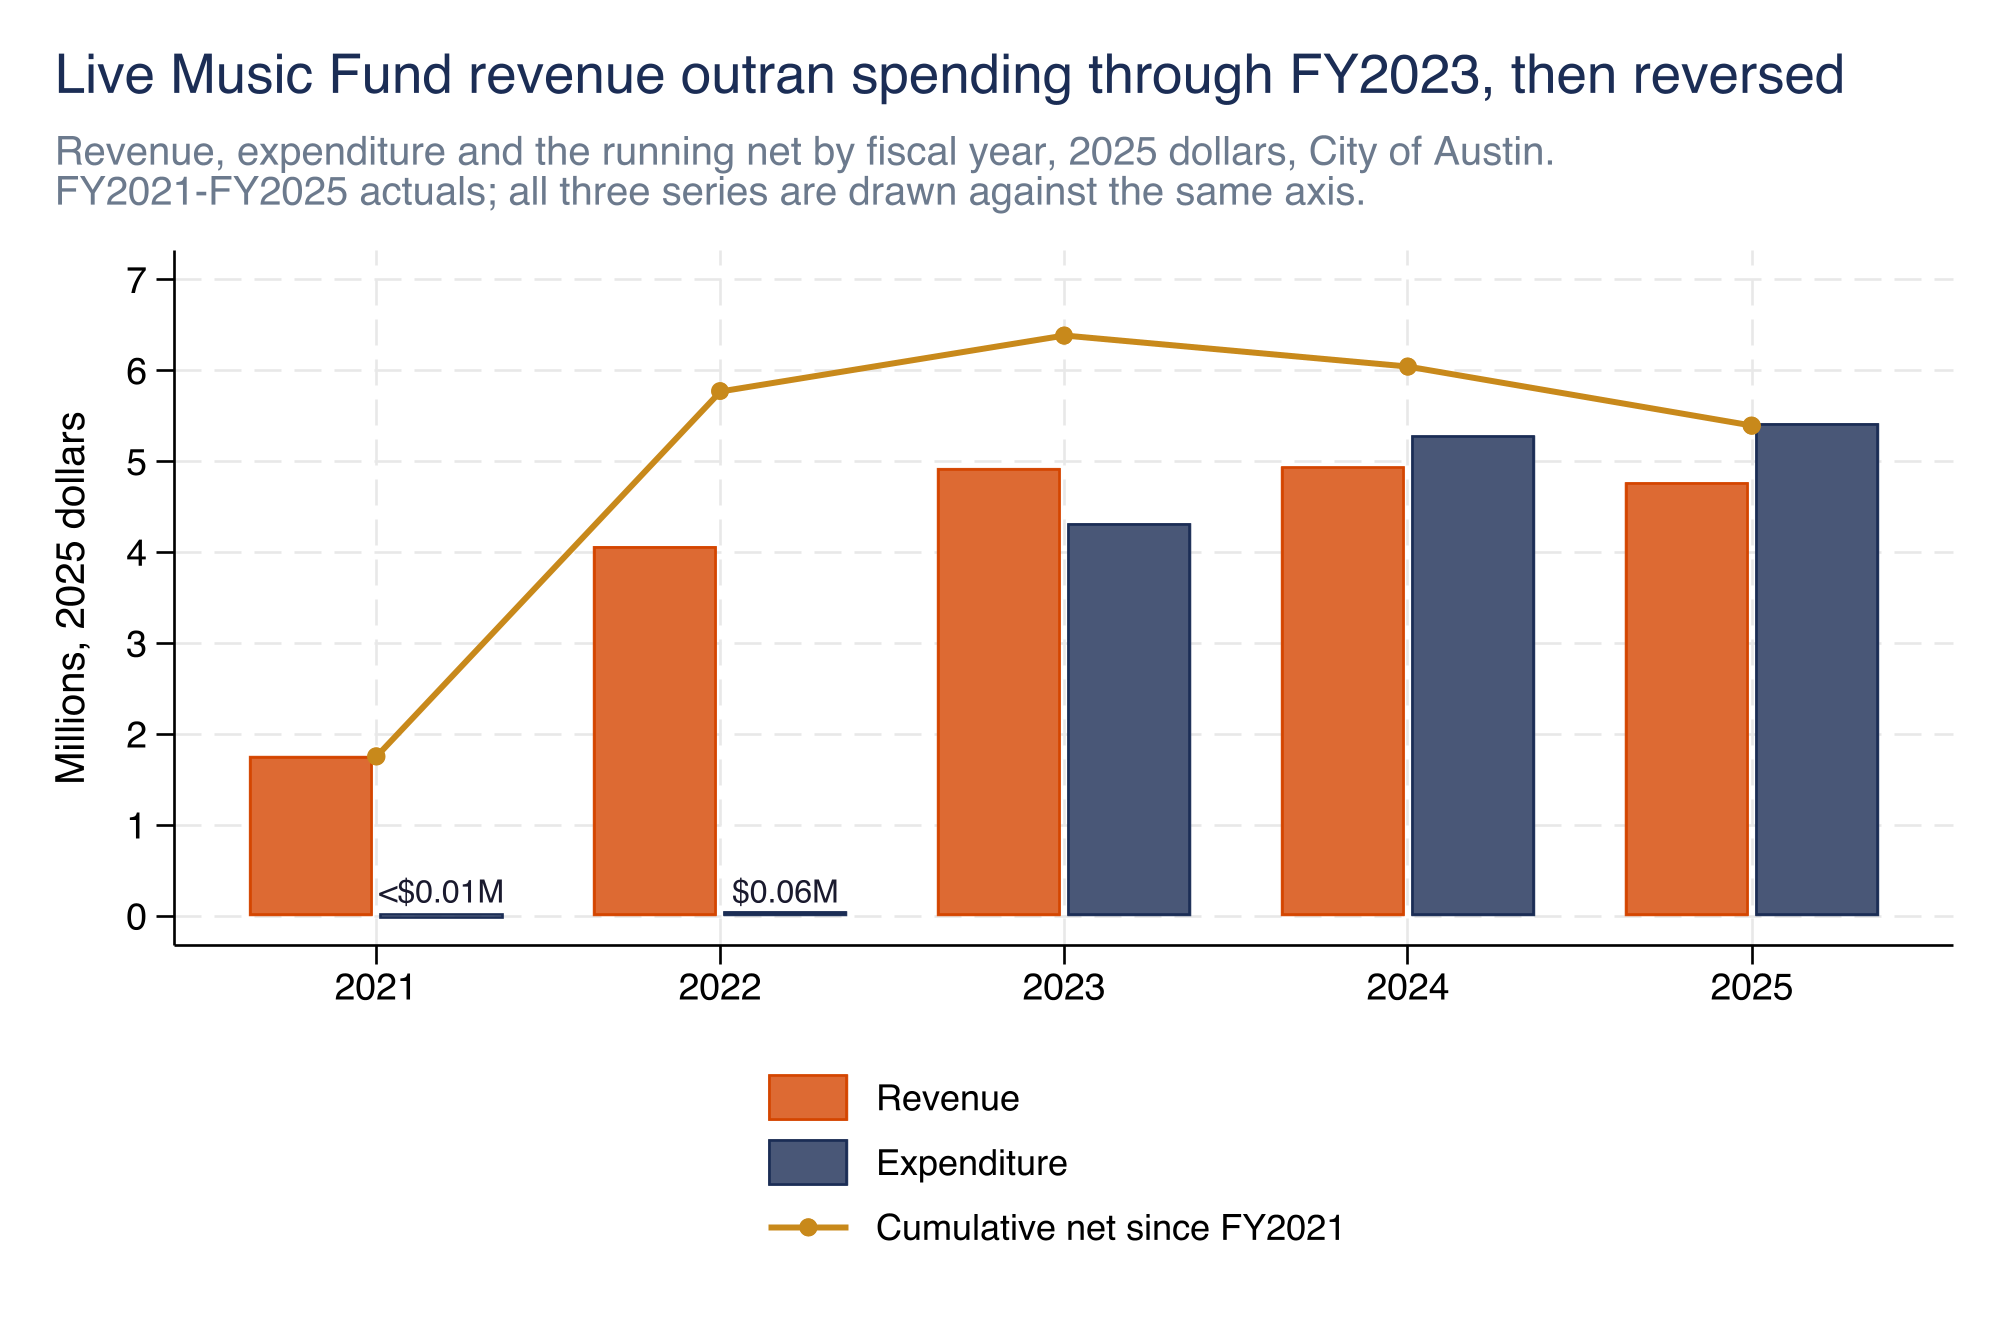
\includegraphics[width=\textwidth]{fig13_lmf_flow.png}
\caption{Live Music Fund revenue against expenditure by fiscal year, 2025
dollars, with the cumulative position on the right axis. Sources: City of
Austin Open Budget ATX, \textit{Revenue Open Budget -- revised} (dataset
5rhv-xasu) and \textit{Expense Open Budget -- revised} (dataset
yeeq-kk6v), Live Music Fund rows for fiscal 2021 through fiscal 2026. How
to read it: bars are annual flows and the line is the running total of
revenue minus expenditure. Caveat: that cumulative line is a cash-flow
proxy built from fiscal 2021 forward, not an audited fund balance. It
excludes any opening balance and does not reconcile with press reporting
that put the fund's balance at roughly \$3.2 million in September 2025, a
gap that cannot be resolved without the city's audited fund-balance
schedule.}
\label{fig:lmfflow}
\end{figure}

The City Council created the Live Music Fund in September 2019 and the
fund did not disburse a substantial grant until fiscal 2023. By the close
of fiscal 2022 the fund had accumulated \NCityLmfAccumByFyTwoTwoNominal\
in unspent nominal money across the period when musicians' income was
most disrupted.\footnote{The Open Budget series begins in fiscal 2021, so
fiscal 2020 collections are not in that figure. The figure is a cumulative
revenue-minus-expenditure proxy built from the two Open Budget extracts
(5rhv-xasu and yeeq-kk6v) rather than an audited fund balance, and it
excludes any opening balance the fund carried from its 30 September 2019
creation. Figure~\ref{fig:lmfflow} plots the same cumulative position in
2025 dollars, where it reaches a higher number for the same fiscal year.
The gap against press reporting of a \$3.2 million balance in September
2025 remains open pending the city's Annual Comprehensive Financial
Report fund-balance schedule.} Innocent explanations for the delay exist:
a new fund has to write eligibility rules, procure an administrator and
stand up an application process, and the pandemic disrupted all three.
The timing still matters. The fund spent \$4,284 in fiscal 2021 and
\$50,000 in fiscal 2022 against \$1.5 million and \$3.7 million in
revenue,\footnote{Annual amounts in this sentence are from the Open Budget
expense (yeeq-kk6v) and revenue (5rhv-xasu) extracts,
\texttt{fund\_nm~=~Live~Music~Fund}, actuals for fiscal 2021 and fiscal
2022.} so almost nothing left the fund during the years musicians' income
was most disrupted.

Of every dollar the fund has spent through fiscal 2026, roughly 13 cents
paid for something other than grants to musicians, venues and promoters:
\NCityLmfAdminShareGrants\ of cumulative spending went to grants to
subrecipients, \NCityLmfAdminShareConsultant\ to the third-party
administrator that runs the application process, and
\NCityLmfAdminShareAdvertising\ to advertising.\footnote{Object-level
actuals for fiscal 2021 through fiscal 2027, summed across years, from the
City of Austin Open Budget ATX expense extract (dataset yeeq-kk6v) with
\texttt{fund\_nm~=~Live~Music~Fund}, retrieved 1 August 2026 from
\url{https://data.austintexas.gov/resource/yeeq-kk6v.csv}. The three
denominated objects are Grants to Subrecipients, Consultant-Others (the
fund's third-party administrator, the Long Center for the Performing
Arts, from fiscal 2023 onward) and Advertising. The Open Budget expense
series carries no Personnel or other object rows for this fund. Fiscal
2026 is a partial-year actual, unclosed at the time of writing, and
fiscal 2027 rows are budget only. Fiscal 2026 figures for the three
shares thus draw on a year that had not closed when this study was
written.}

\subsection{What a musician could receive depended on the year they applied}

\begin{figure}[htbp]
\centering
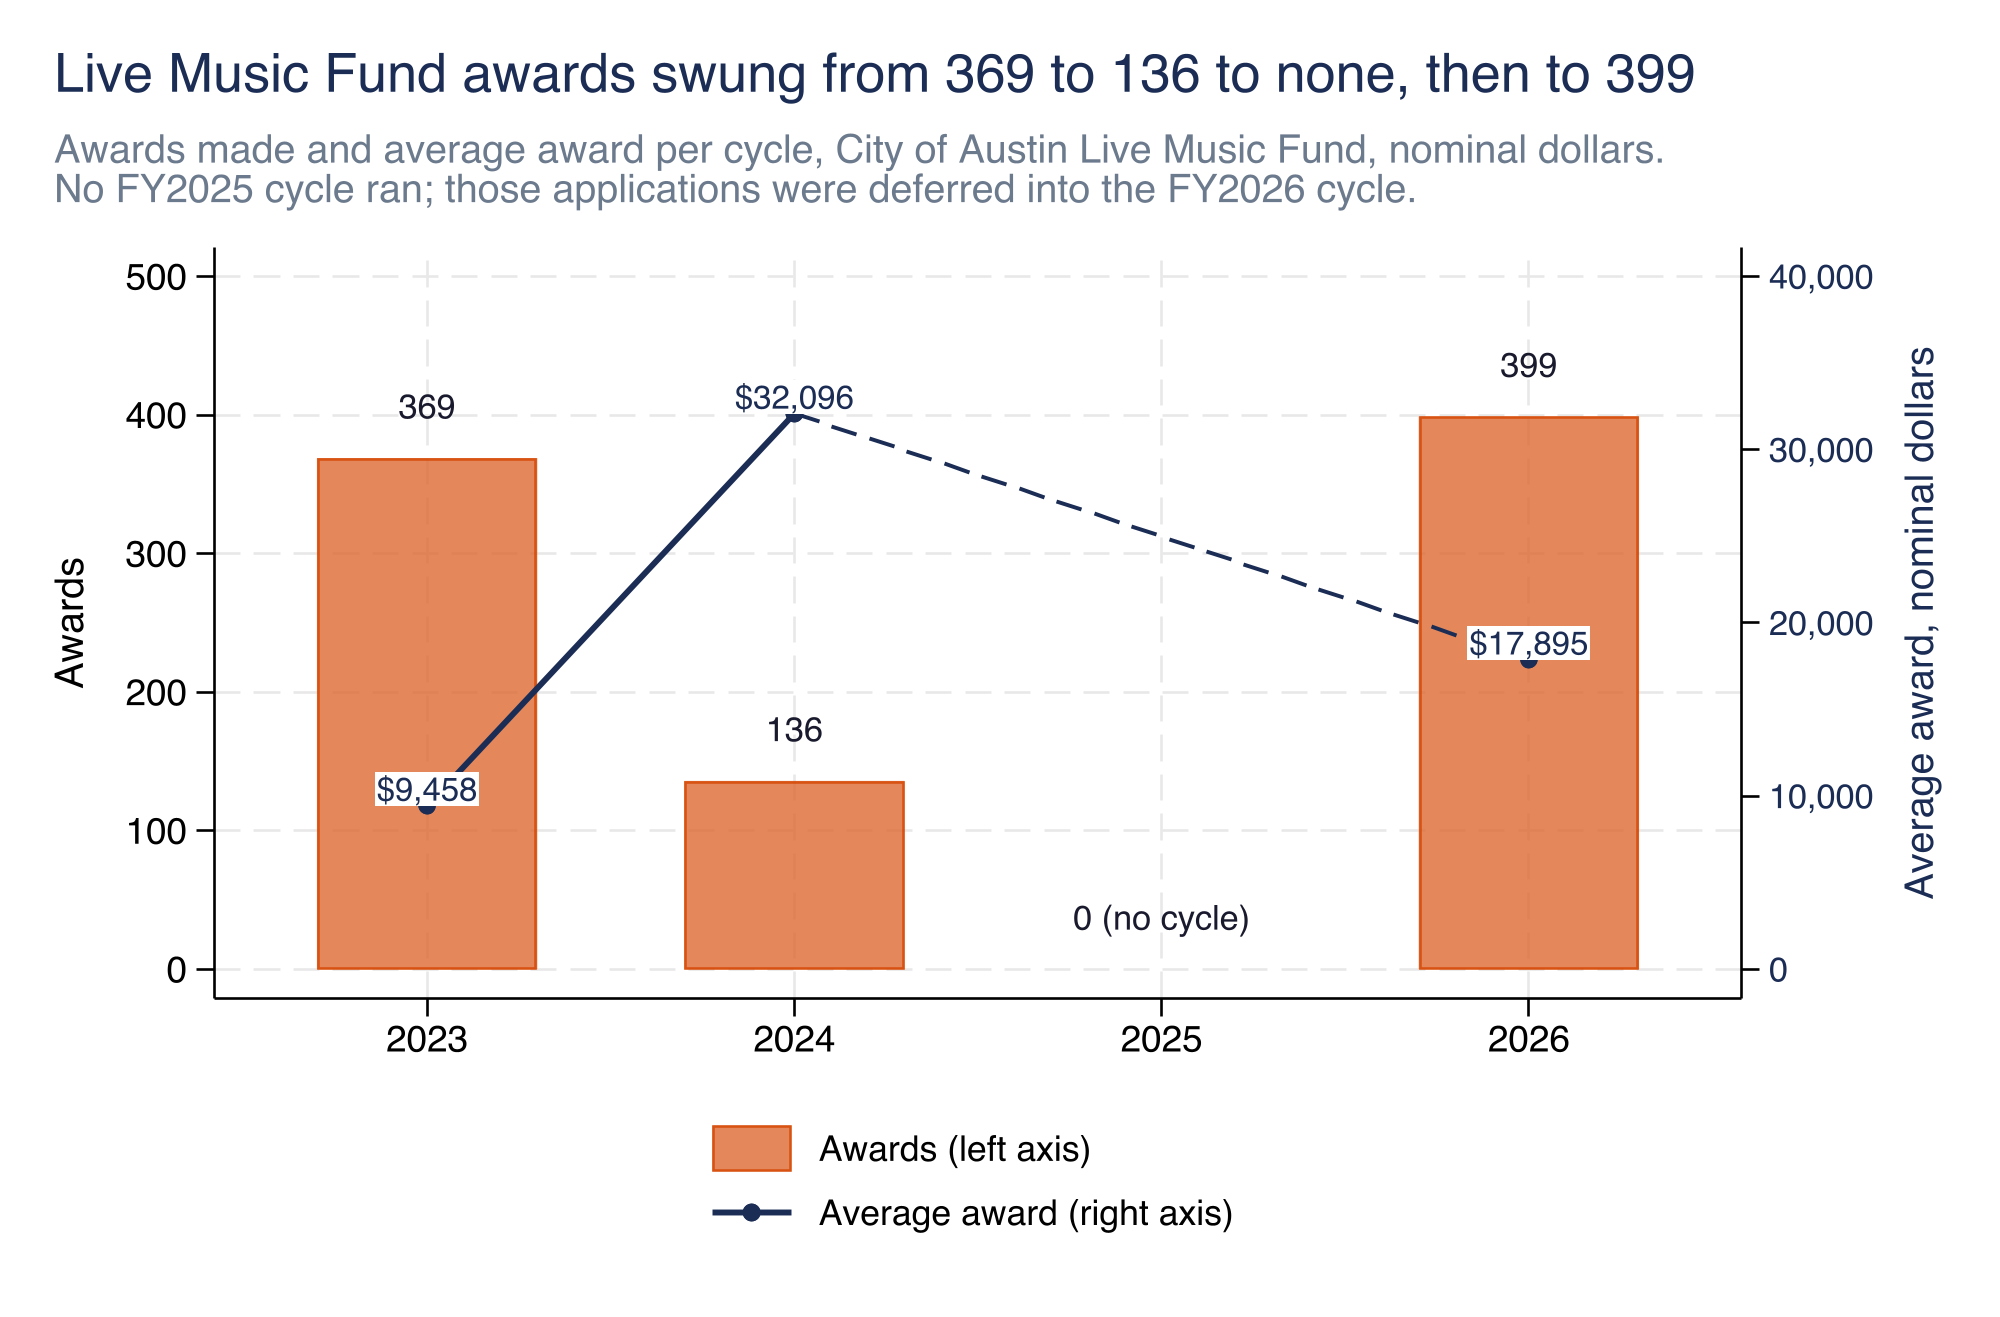
\includegraphics[width=\textwidth]{fig14_lmf_cohorts.png}
\caption{Live Music Fund awards and average award by cycle. Sources: the
city's fiscal 2023, fiscal 2024 and fiscal 2026 awardee lists, using each
document's own stated headline totals, plus the official Live Music Fund
program page for the fiscal 2025 zero. How to read it: bars are the
number of awards on the left axis and the line is the average award on
the right axis, broken rather than interpolated at fiscal 2025 because no
cycle ran that year. Caveats: the fiscal 2023 count is
\NCityLmfFyTwoThreeAwardsList\ in the awardee list PDF against
\NCityLmfFyTwoThreeAwardsPress\ in press reporting, a difference that
appears to be one duplicated name; the fiscal 2026 list does not
reconcile with itself, so its stated headline totals are used here.}
\label{fig:lmfcohorts}
\end{figure}

From one cycle to the next, the average award and the number of
recipients moved in opposite directions, and no cycle ran at all in
fiscal 2025.\footnote{The primary awardee lists this section reads are the
fiscal 2023 Live Music Fund Event Program Awardee List
(\url{https://austin.widen.net/view/pdf/jfxwxsxktx/2023LiveMusicFundEventProgramAwardeeList.pdf?t.download=true}),
the fiscal 2024 Austin Live Music Fund Awardee List
(\url{https://austin.widen.net/view/pdf/bpzuacfkk8/FY24-AwardeeList_Austin-Live-Music-Fund.pdf?t.download=true})
and the March 2026 ACME Funding Program Award List, which covers both
the fiscal 2026 Live Music Fund and the Elevate program
(\url{https://austin.widen.net/s/hhgtdnjqmn/almf_acme-2026-funding-program-award-list}).
The official program page
(\url{https://www.austintexas.gov/atxmusic/live-music-fund}) records zero
awards for fiscal 2025 and describes the cycle as deferred, with
applications folded into the fiscal 2026 round. No applicant count for
the fiscal 2026 Live Music Fund alone has been published; the city's
fiscal 2026 cultural funding news release reports 1{,}606 applicants
requesting more than \$67 million across the four current cultural
funding programs combined (Elevate, Live Music Fund, Creative Space
Assistance Program and Heritage Preservation),
\url{https://www.austintexas.gov/communications/news/city-austin-announces-2026-cultural-funding-awards},
without an individual-fund breakdown. The fiscal 2026 award list is also
inconsistent with itself in three places: it names 21 venues against its
own subtotal of 20; its musician and promoter rows fall
\NCityLmfFyTwoSixMusicianDollarGap; and its headline count of 399 awards
does not match the sum of its two section subtotals,
\NCityLmfFyTwoSixSubtotalCountGap. The share-funded column in the table
below divides press-reported award counts by press-reported applicant
counts, so the numerator differs slightly from the award count shown in
the same row (which is a tally of the city's own list PDF); the fiscal
2024 share also covers musician and promoter awards only, leaving out
that cycle's new venue awards, while the published applicant count it
divides by carries no venue-versus-nonvenue split, so the fiscal 2023 and
fiscal 2024 shares are not strictly comparable.}

\begin{center}
\footnotesize
\begin{tabular}{@{}B{2.6cm} R{2.2cm} R{3.0cm} R{3.6cm}@{}}
\toprule
\textbf{Fiscal year} & \textbf{Awards} & \textbf{Average award} &
\textbf{Share of applicants funded} \\
\midrule
2023 & \NCityLmfFyTwoThreeAwardsList{} & \NCityLmfFyTwoThreeAvg{} &
\NCityLmfFyTwoThreeFundedShare{} \\
\rowrule
2024 & \NCityLmfFyTwoFourAwards{} & \NCityLmfFyTwoFourAvg{} &
\NCityLmfFyTwoFourFundedShare{} \\
\rowrule
2025 & \multicolumn{3}{c}{No cycle ran} \\
\rowrule
2026 & \NCityLmfFyTwoSixAwards{} & \NCityLmfFyTwoSixAvg{} & Not published \\
\bottomrule
\end{tabular}
\end{center}

\vspace{3pt}
For an individual musician that variation is the operative fact: the same
application submitted in two different years faced a different chance of
funding and a different award. Predictability is part of what makes a
grant program useful for people whose income is irregular.

\subsection{Demand for venue capital ran far ahead of supply at the fund's first award}

Section~\ref{sec:venues} showed that Austin loses live-music capacity
when rooms stop reporting and no one replaces them, which points at the
cost of buildings and the security of leases. The Austin Economic
Development Corporation's Iconic Venue Fund is aimed at exactly that: it
helps venues buy or secure their buildings.\footnote{The Iconic Venue
Fund is a capital-preservation program run by the Austin Economic
Development Corporation, a public non-profit created by the city, and it
is distinct from the grantmaking Live Music Fund the rest of this
section reads. It draws on hotel-occupancy-tax revenue and a 2018 bond
package. The 2023-snapshot figures in this paragraph are from Austin
Chronicle reporting on the fund's first award: Genevieve Wood,
\textit{What Hole in the Wall's Freshly Inked 20-Year Lease Means for
Other At-Risk Venues}, 24 August 2023,
\url{https://www.austinchronicle.com/music/2023-08-25/what-hole-in-the-walls-freshly-inked-20-year-lease-means-for-other-at-risk-venues/}.
No primary Austin Economic Development Corporation document publishing
these counts was located, and this study reports the newspaper figures
as secondary.} At its first award in August 2023 the Iconic Venue Fund
had received \NCityIvfProposals\ proposals requesting
\NCityIvfRequested. Its selection committee had shortlisted
\NCityIvfShortlisted\ proposals and had made a single award of
\NCityIvfAwardTwoZeroTwoThree\ to the Hole in the Wall, so the requests
in hand ran to \NCityIvfRequestedToAwardRatio\ the size of that single
award.\footnote{The \$300 million requested figure is a stated floor
rather than an exact total, so the ratio to the single award is at least
the value shown. That figure is a 2023 snapshot rather than the fund's
current state. City Open Budget expense data record cumulative Iconic
Venue Fund grants to subrecipients of \$15.3~million through fiscal 2026
(dataset yeeq-kk6v, \texttt{fund\_nm~=~Iconic~Venue~Fund}), so
substantially more has been awarded since; against that total the \$300
million floor implies a ratio roughly an order of magnitude smaller. The
Austin Economic Development Corporation has not published an updated
proposal count, shortlist or recipient list. Cumulative Open Budget data
also put the fund's revenue minus expenditure at
\NCityIvfCumulativeNetNominalFyTwoSix\ through fiscal 2026, but that
position is produced almost entirely by fiscal 2026, an incomplete year
in which \$2.9 million of spending is recorded against revenue that has
not yet posted; summed through fiscal 2025, where the data are complete,
the fund is net positive.}

The imbalance is not confined to venue capital. In the 2020 Creative
Space Disaster Relief round, \NCityCsapTwoZeroTwoZeroApplicants\
applicants requested about \$3.7 million against the \$1 million
available, which the program page describes as nearly four times the
money on offer
(\NCityCsapTwoZeroTwoZeroOversubVsAvailable).\footnote{City of Austin,
Creative Space Assistance Program page,
\url{https://www.austintexas.gov/creative-space-assistance-program},
retrieved 1 August 2026. The 2020 round funded 32 of the 65 applicants
for \$987{,}943 total, with the awardee mix running to 12 live-music
venues, 11 arts nonprofits, 7 theaters, 1 museum or gallery and 1
individual artist. This 2020 round is the only Creative Space cycle for
which the city has published an applicant count.}

\subsection{No performance audit of the Live Music Fund exists}

The Office of the City Auditor has published no performance audit of the
Live Music Fund. Its one adjacent review, a 2024 special request on
cultural arts funding, states in its own scope that it did not look at
funding for music, and a search of the auditor's report index returns no
music-titled audit.\footnote{City of Austin Office of the City Auditor,
\textit{Special Request: EDD Culture and Arts Funding} (October 2024),
which reports on its own page 2 that ``we did not look at funding for
music or music disaster'' relief:
\url{https://austin.widen.net/view/pdf/pifyu2e2j6/Special_Request_EDD_Culture_and_Arts_Funding_October_2024.pdf?t.download=true}.
The auditor's public index of published reports at
\url{https://www.austintexas.gov/auditor/audit-reports} carries no
title matching the Live Music Fund as of 1 August 2026.} That is a
separate question from the city's annual financial audit, whose
fund-balance schedule would be needed to reconcile the Live Music Fund's
cash position against the press reporting cited in
Figure~\ref{fig:lmfflow}.

In mid-2025, 60 Live Music Fund recipients were out of compliance with
their reporting requirements, \$550,000 in awards was frozen pending
their final reports, and \$70,000 of that had been forfeited
outright.\footnote{Austin Monitor, \textit{Dozens of City Music Grants
Stalled Over Missing Final Reports}, 19 June 2025,
\url{https://austinmonitor.com/stories/2025/06/dozens-of-city-music-grants-stalled-over-missing-final-reports/},
reporting a 16 June 2025 presentation to the Arts Commission. This is
secondary reporting; no primary city document publishing these counts
was located, and no denominator for the 60 non-compliant recipients was
published alongside the count. The \$550,000 figure is the hotel-tax
share of \$847,500 frozen citywide across 70 contracts.}

The absence of a performance audit matters despite the fund's size. The
Live Music Fund is small, but its award rules have
changed in every cycle, its administration has moved to a third party,
and its cash position cannot be reconciled against public reporting
using open data alone. Those are the conditions under which a periodic
audit is normally expected.

The Live Music Fund is the city's main direct instrument for music, and it
is one of several public levers this workforce faces. Section~\ref{sec:state}
turns to the state and federal ones: the Texas Music Incubator Rebate
Program the Governor's office administers, the arts-economy aggregate the
Bureau of Economic Analysis publishes at the state level, and the federal
Shuttered Venue Operators Grant program that was the largest single
intervention of the period.

% Section 7: Texas in context. Balanced: the state's program is small but fully
% spent, which is more than several peers can say.
\section{Texas commits little to music, and awarded all of it in the one round it has published}
\label{sec:state}

Austin's fund is not the only public money aimed at this workforce, and the
state's works differently. The Texas Music, Film, Television and Multimedia
Office, an office in the Governor's office of Economic Development and Tourism,
administers both the music rebate and the state's moving-image incentive under
Chapter 485 of the Government Code.\footnote{Government Code Chapter 485
places the Music, Film, Television and Multimedia Office inside the Governor's
Economic Development and Tourism division and gives it authority to administer
both incentive programs. That statutory location is why the same office serves
as the state actor across the film-and-television, film-workforce, and music
programs compared below.}
Placing those dedications beside one another shows what the state has committed
to each. This section then compares Texas with four peer states (Georgia, New
York, Tennessee, Louisiana) on music money awarded, claimed or appropriated
rather than merely authorised, sets the Texas arts economy beside the national
aggregate, and ends with the federal pandemic relief program that was the
largest single intervention of the period.

\subsection{The same state office commits far more to film than to music}

\begin{figure}[htbp]
\centering
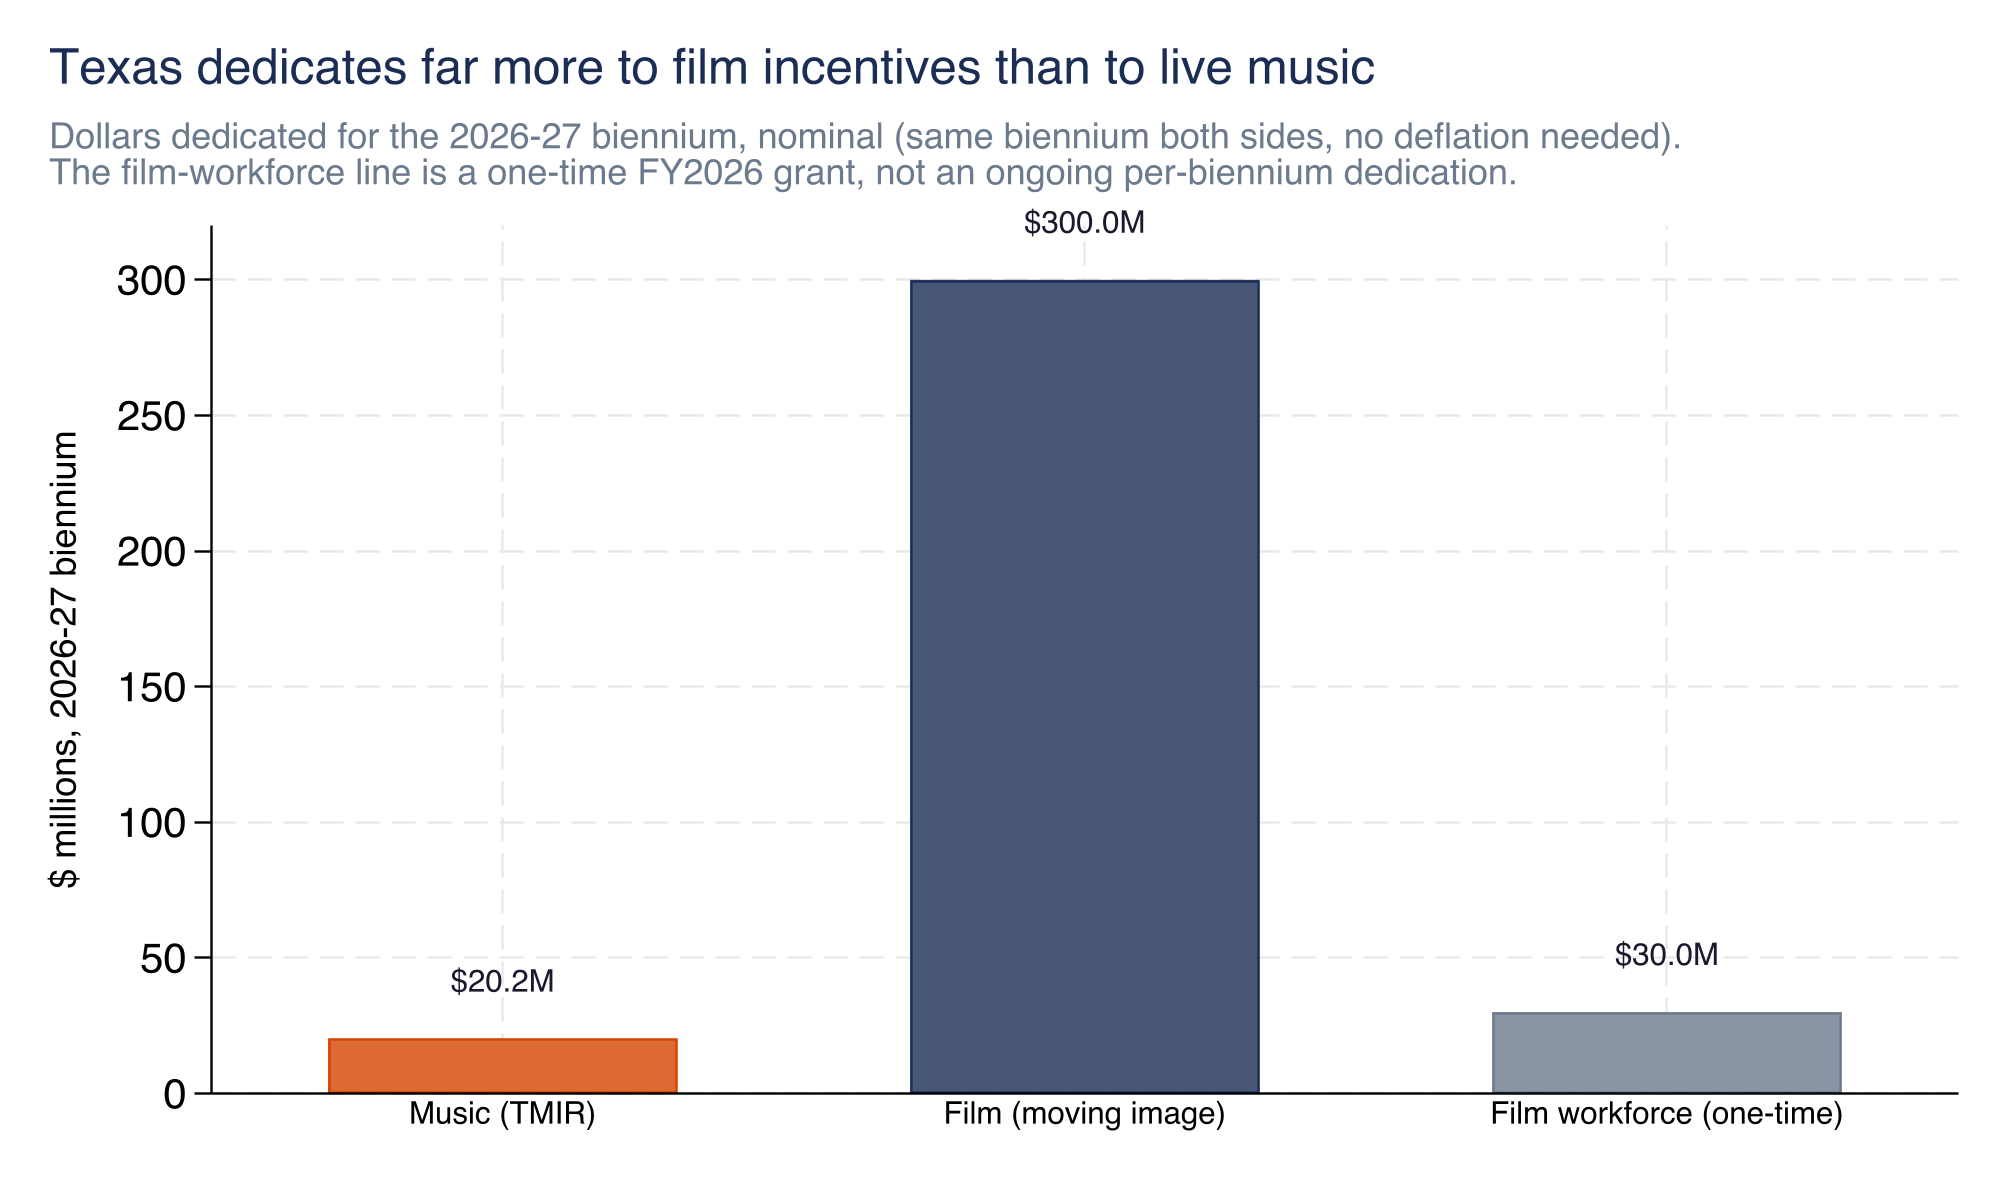
\includegraphics[width=0.86\textwidth]{fig15_film_vs_music.png}
\caption{Texas dedications for the 2026--27 biennium, nominal dollars. Sources:
General Appropriations Act riders; Senate Bill 22, 89th Legislature, 2025. How
to read it: all three amounts are dedicated for fiscal 2026--27, so they are
already in comparable nominal terms and no inflation adjustment is needed.
Caveat: the film workforce line
is a one-time fiscal 2026 grant to universities rather than an ongoing
per-biennium dedication, it has no music counterpart, and it is never summed
with the other two.}
\label{fig:filmmusic}
\end{figure}

The 89th Texas Legislature dedicated \NTxFilmIncentiveBiennium\ to the
moving-image incentive for the 2026--27 biennium through Senate Bill 22, and
dedicated \NTxMusicTmirBiennium\ to the Texas Music Incubator Rebate over the
same two years under the earlier statute that created it. The ratio between the
two dedications, both nominal dollars for the same fiscal biennium, is
\NTxFilmMusicRatio.\footnote{The moving-image incentive appears at Texas Tax
Code section 151.801(g), added by Senate Bill 22 of the 89th Legislature
(2025), which requires the Comptroller to deposit \$300{,}000{,}000 per
biennium into the fund and sunsets on 1 September 2035. The music rebate
appears at Tax Code sections 183.023(c) and 151.801(f), added by Senate Bill
609 of the 87th Legislature (2021), which together dedicate
\$10{,}100{,}000 a year to the rebate account beginning with the 2024--25
biennium; Rider 39 or 40 of the General Appropriations Act appropriates that
amount to the Music Office each biennium. Because both figures are nominal
dollars for fiscal 2026--27, no inflation adjustment applies to their ratio.
Statutory materials at
\url{https://capitol.texas.gov/BillLookup/History.aspx?LegSess=89R\&Bill=SB22}
and the Comptroller's Manual of Accounts entry for the music account at
\url{https://fmcpa.cpa.state.tx.us/fiscalmoa/fund.jsp?num=5193}.}
The Texas Music Incubator Rebate, unlike its peer credits in other states,
returns a portion of mixed-beverage and sales taxes that a qualifying venue or
promoter has already remitted to the Comptroller, so the subsidy scales with a
venue's alcohol sales rather than with what the venue pays performers. The
authorising statute requires that a written artist contract exist but sets no
minimum compensation.\footnote{The Legislature created the rebate in Senate
Bill 609 in 2021 and left it unfunded until 2023, and the first application
window opened on 1 September 2023.} The same 2025 legislative session that
increased film also authorised a \NTxFilmWorkforcePilotOnetime\ Higher
Education Film Workforce Pilot Program under Rider 45 of the 2026--27 General
Appropriations Act, a one-time fiscal 2026 grant to universities for film and
media workforce training with no music counterpart.\footnote{Rider 45 restricts
the \$30{,}000{,}000 of General Revenue to eligible general academic teaching
institutions and to film and media workforce activities specifically, and
prohibits its use for any other purpose. Registered as one-time so it is never
summed with the recurring biennial moving-image or music dedications.}

\subsection{A statutory cap is not a measure of support}

\begin{figure}[htbp]
\centering
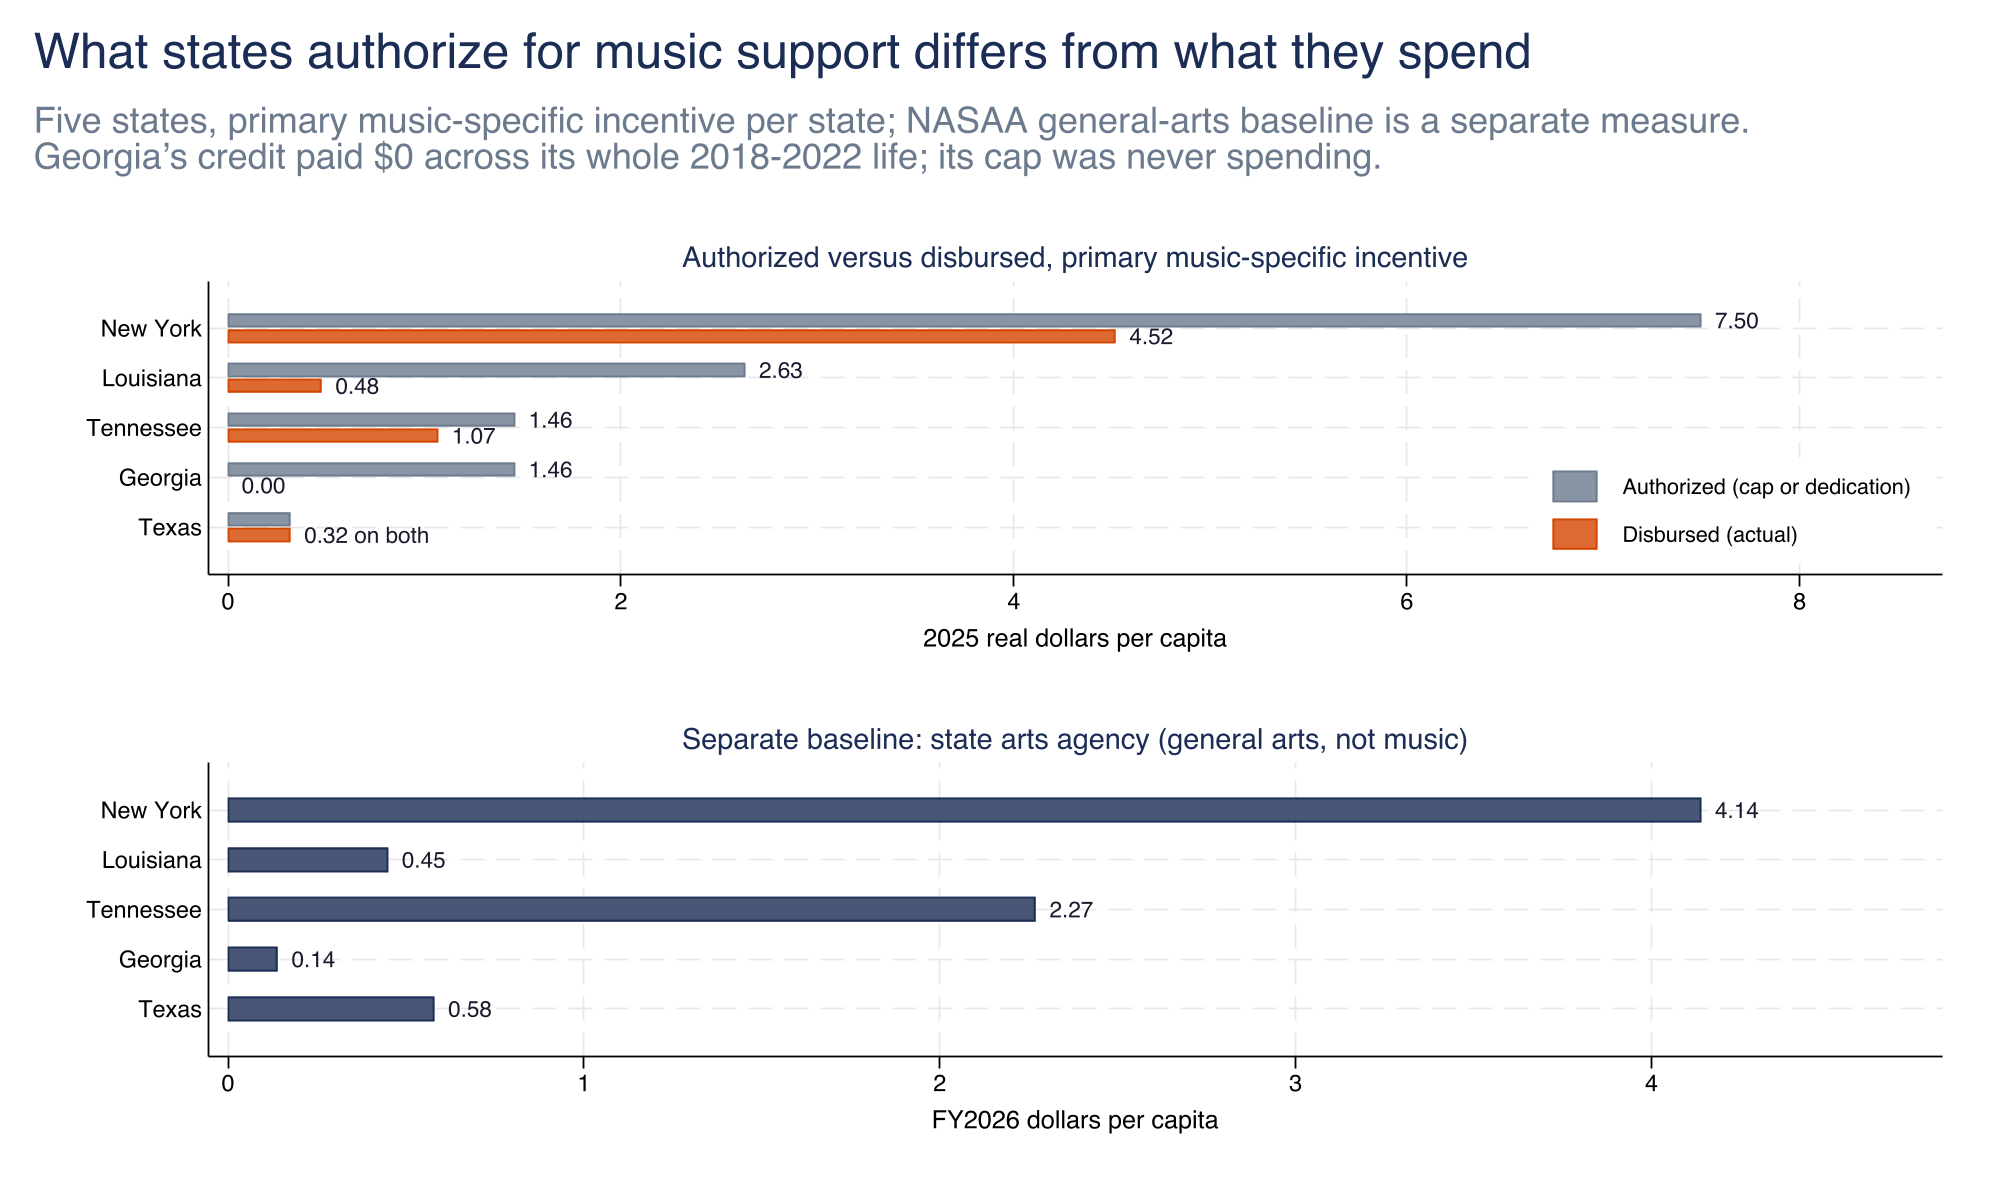
\includegraphics[width=\textwidth]{fig16_state_percapita.png}
\caption{State music incentives per resident, authorised against actually
awarded, claimed or appropriated, five states, 2025 dollars, with general state arts agency funding
shown separately below. Sources: state statutes and agency reports; National
Assembly of State Arts Agencies; Census Bureau population estimates for July
2025. How to read it: the upper panel shows what each state's music-specific
program allows against what it paid, and the lower panel is general arts
funding, a different measure that does not add to the upper one. Caveats:
the New York authorised figure is a proxy derived from a budget increase rather
than a flat annual cap; the Tennessee bars combine film, television and music
scoring with no music-only breakout available, so they are an upper bound.}
\label{fig:statepercap}
\end{figure}

The Georgia General Assembly authorised up to \$15 million a year for a music
tax credit under O.C.G.A.\ section 48-7-40.33, and the Georgia Department of
Revenue paid out nothing over the credit's five-year active life. The Georgia
Department of Audits and Accounts, in a December 2023 evaluation, found that
the department received six applications and approved none, because each
lacked the required pre-certification from the Georgia Department of Economic
Development.\footnote{Georgia Department of Audits and Accounts and Georgia
Southern University CBAER, \textit{Georgia Music Tax Credit: Economic and
Fiscal Impact Analysis}, report dated 8 December 2023, published 14 December
2023, at
\url{https://www.audits.ga.gov/ReportSearch/download/30448}. The state's
published Tax Expenditure Reports listed the credit as ``less than
\$1 million,'' a notation that concealed a true value of zero.} On the
statutory ceiling alone, Georgia's music support looks larger than Texas's;
on dollars actually paid, Georgia is at
\NMusicDisbursedPercapitaGeorgia\ per resident.

On money awarded, claimed or appropriated per resident rather than authorised,
Texas is at \NMusicDisbursedPercapitaTexas\ against New York's
\NMusicDisbursedPercapitaNewyork\ and Louisiana's
\NMusicDisbursedPercapitaLouisiana. Tennessee's
\NMusicDisbursedPercapitaTennessee\ combines film, television and music
scoring together in the Tennessee state budget's single Film and Television
Incentive Fund line, and so cannot be ranked against a music-only figure.
Georgia paid nothing at all. Among the states here whose figures are
music-specific, Texas's dedication is the smallest per resident of those that
paid anything.\footnote{The per-resident figures divide two different
dollar quantities by the same population base. Authorised per resident is
\(a_s = A_s\,d_{y(A_s)} / N_s\) and disbursed per resident is
\(b_s = B_s\,d_{y(B_s)} / N_s\), where \(A_s\) is the annual amount state
\(s\) may award under the statute or dedication behind its music-specific
program, \(B_s\) is the amount the state actually paid or certified,
\(d_y = C_{2025}/C_y\) carries each figure from its own nominal year to 2025
dollars using the national CPI-U, and \(N_s\) is the state's resident
population on 1 July 2025 from the Census Bureau's Vintage 2025 state
population totals at
\url{https://www2.census.gov/programs-surveys/popest/datasets/2020-2025/state/totals/NST-EST2025-ALLDATA.csv}.
The two figures can differ by the entire amount, because an authorisation is a
ceiling written into law and a disbursement is money that left the treasury.
Georgia shows the gap at its widest, with a positive ceiling and nothing paid.
Where a state's authorisation is not a flat annual cap, the figure is a proxy:
the New York number is the most recent one-year budget increase to a
multi-year lifetime cap under Tax Law section 24-c, and the Tennessee figure
combines film, television and music scoring because the Tennessee Department
of Finance and Administration reports no music-only breakout at line 330.17 of
the state budget document, so both are upper bounds. Three cautions apply to
the second column. Only the Texas and Georgia figures are money awarded that
this study could verify against agency award files; the New York, Tennessee
and Louisiana figures are respectively an annualised award total, a
combined-fund appropriation and a claimed credit, so the column is not a
like-for-like disbursement measure. The New York figure annualises
\$308 million in credits awarded between August 2022 and February 2026 (three
and a half years) into a one-year equivalent, against a single Texas rebate
round. The Louisiana figure combines the Sound Recording Investor Tax Credit
at Louisiana Revised Statute 47:6023 with the Musical and Theatrical
Production Credit at R.S. 47:6034; the Sound Recording credit alone is about
\$0.01 per resident, well below Texas. These are accounting ratios built from
published totals, not estimates, and no sampling error attaches to them.
Program-page URLs and the underlying budget documents are consolidated in the
technical appendix under each state name.}

The comparison misses how differently the Texas program is built. In the one
rebate round with a published total, fiscal 2026, the Music Office awarded its
full annual dedication, which no peer state here did. The fiscal 2025 round
total has not been published, and the first round's total is internally
inconsistent, so ``full spending'' describes one documented round rather than a
program-level record. Texas is also the only state compared here that
subsidises operating music venues at all: the peer credits fund production
companies mounting touring or Broadway-style shows, a different instrument
aimed at a different beneficiary.\footnote{The five-state comparison is
therefore not a league table. New York's musical and theatrical production
credit at Tax Law section 24-c subsidises productions; Tennessee's
music-related incentive is a film-scoring subsidy under the 2018 Visual
Content Modernization Act, and the Tennessee Entertainment Commission's
program guidelines expressly declare music videos ineligible. Louisiana's two
credits (sound recording investment and musical and theatrical production)
subsidise recording sessions and touring productions respectively. Only the
Texas rebate pays the operating room itself.}

\subsection{Texas has a small arts economy relative to its size}

\begin{figure}[htbp]
\centering
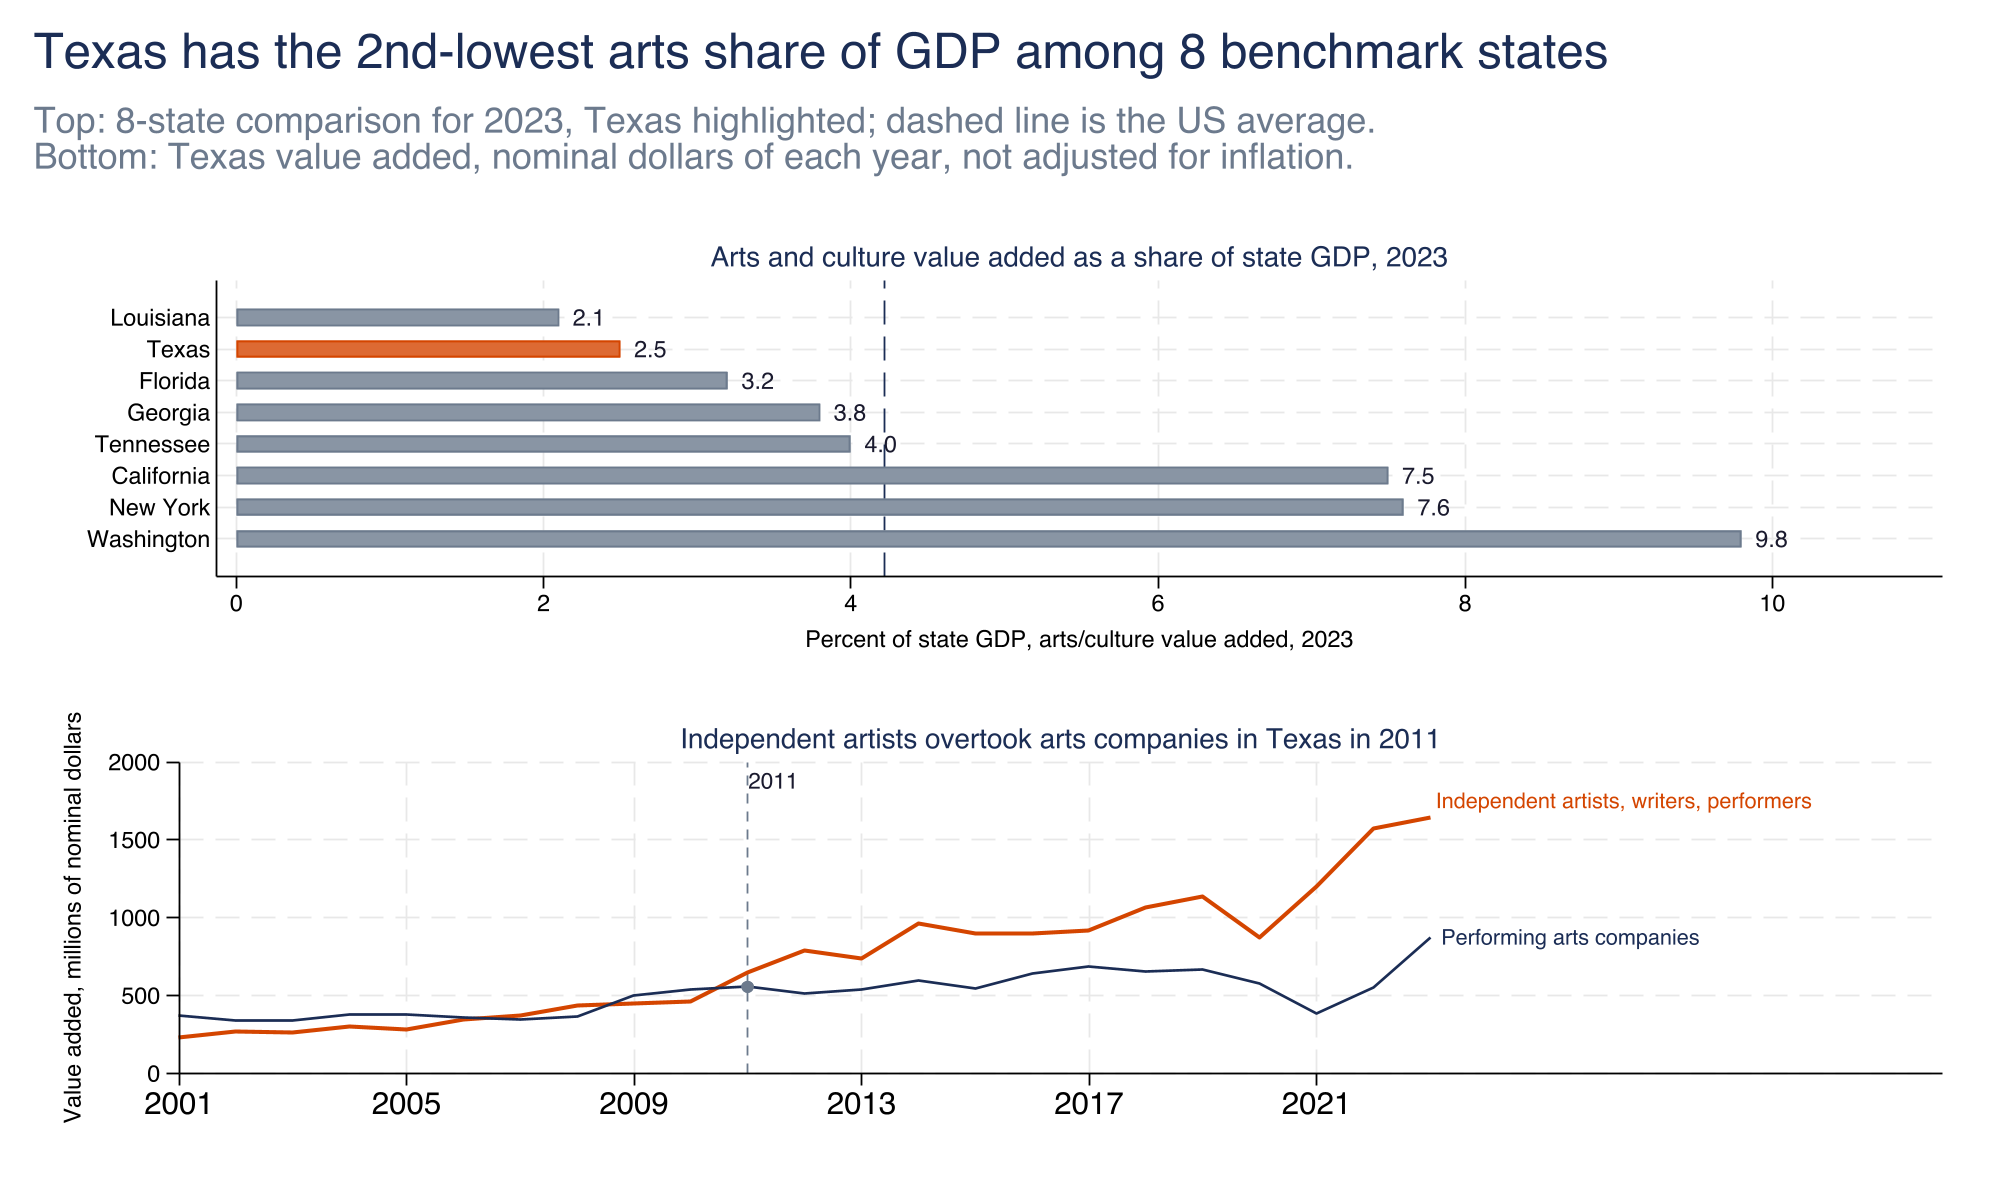
\includegraphics[width=\textwidth]{fig17_bea_arts.png}
\caption{Arts and cultural production as a share of state economic output, eight
states, 2023; and Texas value added for performing arts companies against
independent artists, writers and performers, 2001--2023. Source: Bureau of
Economic Analysis Arts and Cultural Production Satellite Account, nominal
dollars. How to read it: the upper panel compares the eight benchmark states
only, not all fifty. Caveat: this account has no metro-level detail, so it says
nothing about Austin specifically.}
\label{fig:beaarts}
\end{figure}

The Bureau of Economic Analysis publishes the Arts and Cultural Production
Satellite Account, an annual accounting series that measures the value added
by a defined set of arts and cultural industries against total gross domestic
product; the account is the only official U.S.\ statistic that isolates the
economic size of the arts sector at the state
level.\footnote{The BEA account, generally abbreviated ACPSA, uses production
categories built from the North American Industry Classification System and
covers roughly 35 industries from performing arts and museums to
architecture, publishing and broadcasting. Its state file at
\url{https://www.bea.gov/data/special-topics/arts-and-culture} is a
top-down allocation of national commodity totals to states and does not
resolve below the state level, so it cannot describe Austin specifically. The
2023 estimates released on 2 April 2025 in BEA news release 25-13 are the
latest available. The share it produces is the appropriate measure of an
industry's size within a state economy because it deflates the industry to
that state's own economic base, which lets a comparison across states control
for the size of the state.} Arts and cultural production is
\NBeaGdpShareTxTwoZeroTwoThree\ of Texas economic output in 2023, against
\NBeaGdpShareUsAvgTwoZeroTwoThree\ for the United States as a whole. The
United States figure is the national aggregate ratio (all U.S.\ arts value
added divided by total U.S.\ GDP) rather than the mean of the fifty state
shares.\footnote{The share for state \(s\) is
\(100 \times V_s / Y_s\), where \(V_s\) is nominal value added by arts and
cultural production industries in state \(s\) and \(Y_s\) is that state's
nominal total gross domestic product, both in 2023. A ratio of two same-year
dollar figures needs no inflation adjustment, because deflating numerator and
denominator by the same factor leaves the ratio unchanged. Among the eight
benchmark states plotted (California, Florida, Georgia, Louisiana, New York,
Tennessee, Texas and Washington), only Louisiana ranks lower than Texas, at
\NBeaGdpShareLaTwoZeroTwoThree. Nationally, Texas ranks
\NBeaGdpShareTxNationalRank\ across all 50 states and the District of
Columbia; this ranking is taken from BEA's own release rather than re-derived
here, since this study's extract holds only the eight benchmark states and
does not permit an independent national ranking.} The composition inside the
Texas total has also shifted. Value added by independent artists, writers and
performers in Texas first overtook that of performing arts companies in
\NBeaFirstCrossoverYearTx, fell back behind performing arts companies for two
years, then passed it for good in \NBeaCrossoverYearTx\ and has led every year
since. The same movement from institutions toward individuals that
Section~\ref{sec:payroll} found in payroll employment appears here in output.

The Bureau of Economic Analysis posted a notice in February 2026 stating that
it will no longer regularly produce the Arts and Cultural Production
Satellite Account, and so the April 2025 release covering 2023 is the last
year available and no further annual update is
scheduled.\footnote{BEA site text, ``BEA will no longer regularly produce these
statistics,'' February 2026, retrieved 1 August 2026 from
\url{https://www.bea.gov/data/special-topics/arts-and-culture}, cross-checked
against the April 2025 release (BEA news release 25-13). BEA has not ruled
out a future non-regular release, so this is a discontinued schedule rather
than a closed series.}

\subsection{Federal relief was the largest intervention, and it was one-off}

\begin{figure}[htbp]
\centering
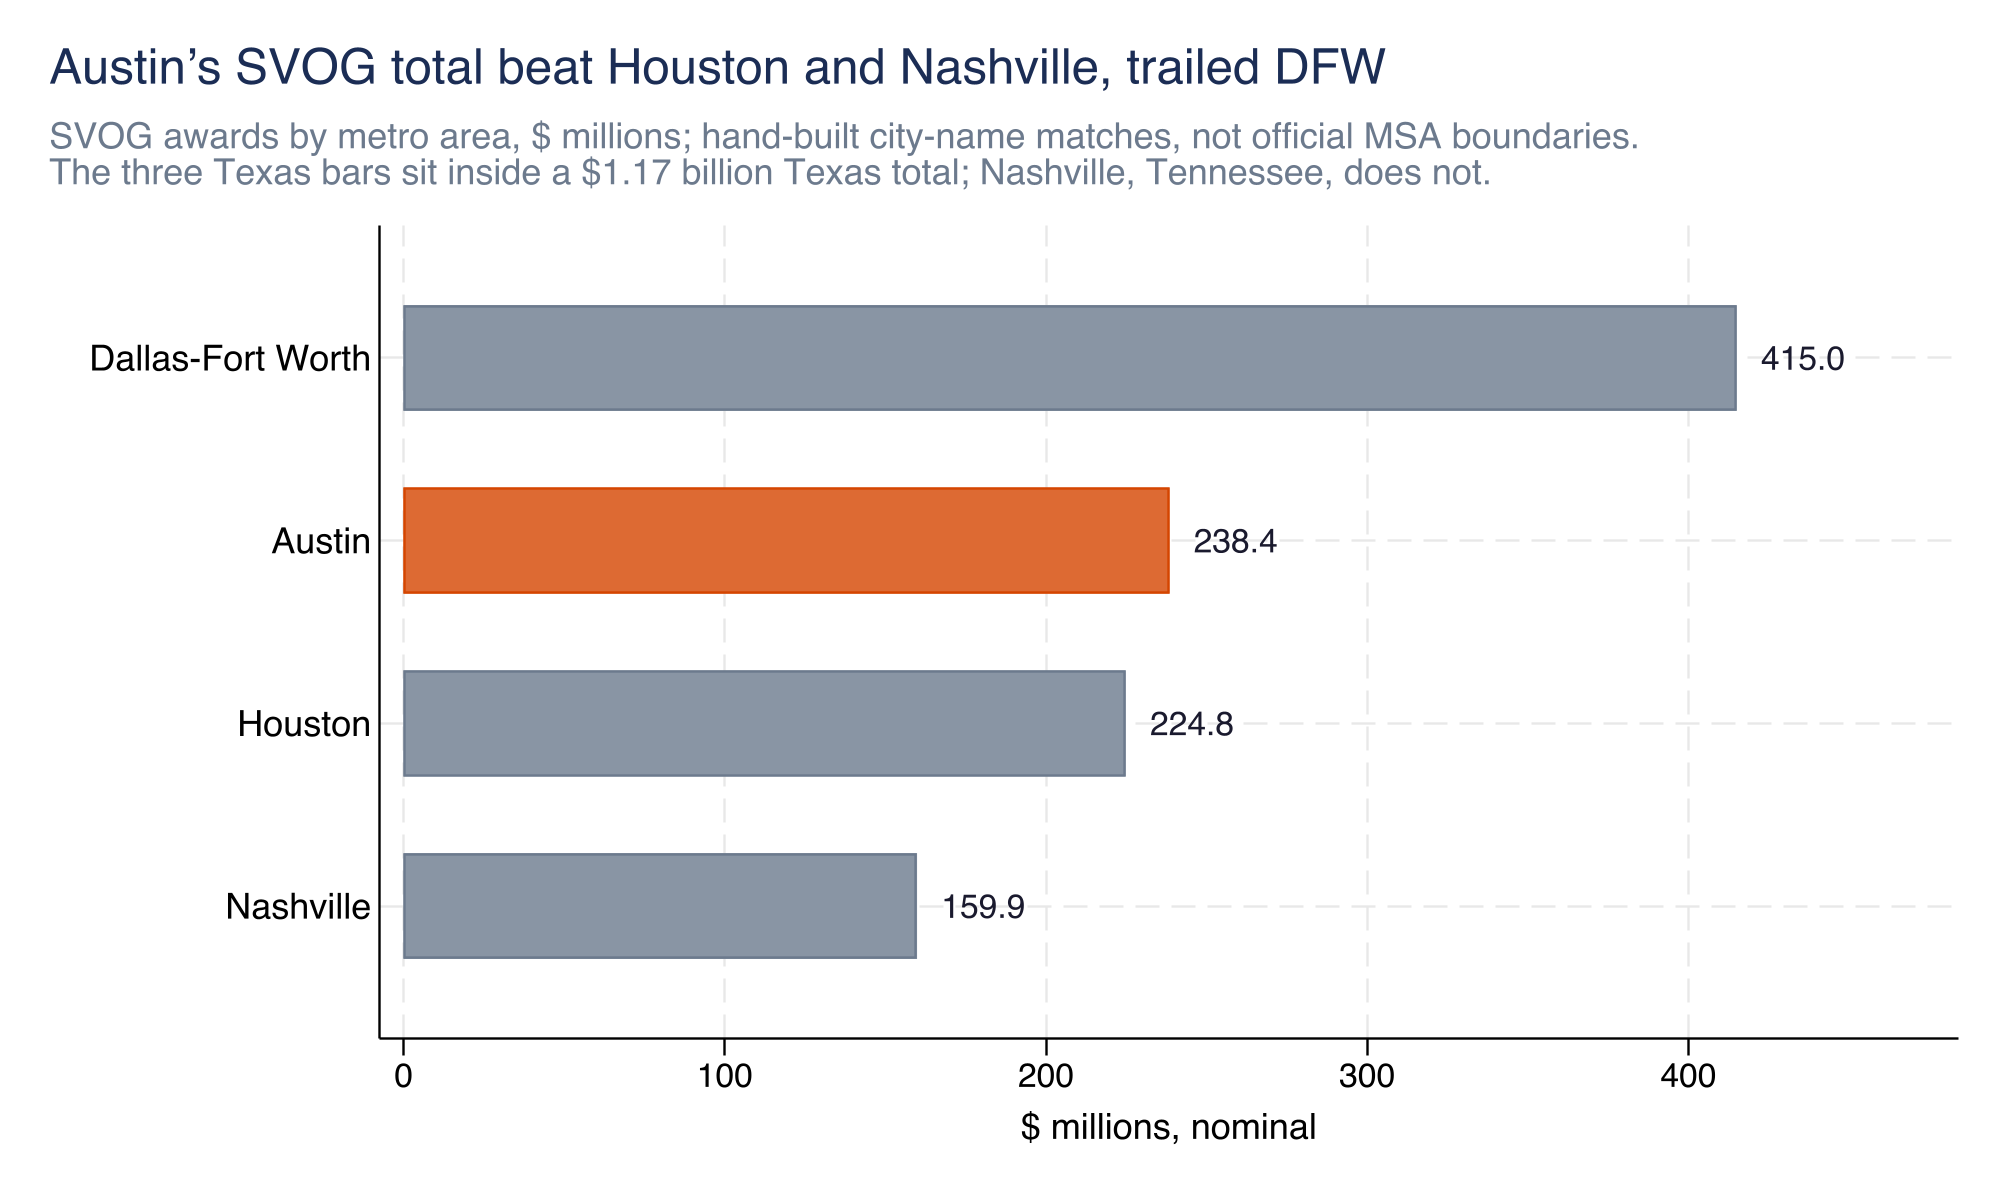
\includegraphics[width=0.86\textwidth]{fig18_svog_metro.png}
\caption{Shuttered Venue Operators Grant awards by metro area. Source: Small
Business Administration award file, July 2022 vintage, the last published. How
to read it: bars are total awarded dollars, nominal. Caveats: metro groupings are built
from recipient city names rather than official metropolitan boundaries, so they
are approximate and will differ from other researchers' groupings for the same
metros; recipient city is the filer's mailing address, so a multi-site chain
books grants for out-of-state locations to its headquarters city; the Nashville
figure covers the consolidated city only while the two Texas figures use
multi-place lists; and the Austin total covers every eligible entity type, of
which motion picture theatre operators account for \$109.8 million across 24
recipients against \$104.9 million to 80 live venue operators and promoters.}
\label{fig:svog}
\end{figure}

Congress created the Shuttered Venue Operators Grant program in December 2020
to compensate live venue operators, promoters, theatrical producers and
motion picture theatre operators for revenue lost during the pandemic
closures; the Small Business Administration administered the program and
published the award file used here.\footnote{The Small Business
Administration award file used here, ``Awards as of 07-05-2022,'' is the
last public release SBA has posted to its open data portal at
\url{https://data.sba.gov/sites/default/files/distribution/SBA-ODA-2022-09-001/awards-as-of-7-5-22.xlsx};
it holds 13{,}011 recipient records nationally. The program's authorising
statute, section 324 of the Economic Aid to Hard-Hit Small Businesses,
Nonprofits, and Venues Act (division N of the Consolidated Appropriations
Act, 2021), capped awards at ten million dollars per entity and gave
priority to operators reporting the deepest revenue drops. Documentation at
\url{https://www.congress.gov/crs_external_products/R/PDF/R46689/R46689.5.pdf}
and \url{https://www.sba.gov/article/2025/01/15/new-report-shows-consequential-impacts-sba-pandemic-relief}.}
Austin-area recipients received \NSvogAustinTotal\ in federal shuttered-venue
grants, against \NSvogHoustonAreaTotal\ for this study's Houston-area
grouping, \NSvogNashvilleTotal\ for Nashville and \NSvogDfwAreaTotal\ for
Dallas-Fort Worth. The Austin and Houston figures should not be ranked
against one another. Three awards inside the Austin group, together worth
\$16.5 million, are filed at Round Rock and Austin corporate addresses but
name cinemas in Iowa, Indiana and Virginia; removing them alone puts Austin
below Houston. Money was concentrated: the top ten Austin recipients
received \NSvogAustinTopOneZeroShare\ of Austin dollars, and
\NSvogAustinCapHits\ reached the program's \$10 million per-entity
cap.\footnote{The concentration measure is
\(100 \times \sum_{j=1}^{10} G_{(j)} \big/ \sum_{j} G_j\), where \(G_j\) is the
awarded amount for recipient \(j\) in the Austin group and \(G_{(1)} \ge
G_{(2)} \ge \dots\) are the same awards sorted from largest to smallest, so
the numerator is the ten largest awards and the denominator is every Austin
award. Award dollars are nominal and are not deflated, because all awards
fall in the same program period. The Austin group is built from recipient
city names rather than official metropolitan boundaries, so the denominator
is this study's grouping and will differ from another researcher's using a
different city list.}

The event study around those awards illustrates why relief programs resist
causal evaluation. In the six months before their award, recipient venues
were running about 39 percent below comparison venues on log monthly
mixed-beverage receipts, with a 95 percent confidence interval that stretched
from about 58 percent below to 12 percent below. The half-year before that is
estimated too imprecisely to distinguish from no gap. Recipients then
converged to no measurable difference from comparison venues after the award.
The pre-award trough looks like the shape of a program effect, but SVOG
eligibility required documenting a revenue drop, so the pre-award trough is
the selection rule made visible in the data rather than an independent
finding of harm.\footnote{The event study runs on half-year blocks measured
from each venue's own award month:
\[
\ln R^{\mathrm{real}}_{it}
  = \alpha_i + \tau_t
  + \sum_{b \neq b_0} \beta_b\,
    \bigl(\mathbf{1}\{\mathrm{block}_{it} = b\} \times \mathrm{SVOG}_i\bigr)
  + \varepsilon_{it},
\]
where \(R^{\mathrm{real}}_{it}\) is venue \(i\)'s monthly receipts in 2025
dollars from the Texas Comptroller Mixed Beverage Gross Receipts dataset
(naix-2893 on the Texas Open Data Portal at
\url{https://data.texas.gov/dataset/Mixed-Beverage-Gross-Receipts/naix-2893}),
\(\mathrm{SVOG}_i\) is one for a matched relief recipient,
\(\mathrm{block}_{it} = \lfloor (t - a_i)/6 \rfloor\) places month \(t\) in a
half-year block relative to that venue's own award month \(a_i\), clipped at
nine blocks before and eight after so the end blocks hold several months for
every award cohort rather than a sliver, and \(\alpha_i\) and \(\tau_t\) are
venue and calendar-month fixed effects respectively. The omitted block
\(b_0\) covers 30 to 25 months before the award, which for the typical award
month is the first half of 2019; the conventional base of the period just
before treatment would fall in the deepest part of the pandemic and would
leave every other coefficient unreadable. Venues that never received an
award are assigned the base block, so they contribute to the fixed effects
and the common time path rather than to any \(\beta_b\). Standard errors are
clustered by venue, and the largest ticketed rooms are excluded. The
p-value quoted below is a joint Wald test that the block coefficients
closing before January 2020 are all zero (the blocks that predate the
pandemic shock for every award month in the data). The pre-pandemic trends
for the two groups are not distinguishable
(\(p = \)~\NQuasiSvogPretrendPPrepandemic), the strongest parallel-trends
evidence in this study, and even so the design still cannot support a causal
claim about the awards themselves. This study matched
\NQuasiSvogMatchedVenues\ Austin awards to the curated venue panel and
dropped three matches as uncertain, with the reasons recorded in the
analysis files. The awards all arrived within a three-month window in
2021, so relative time and calendar time are close to relabellings of one
another.}

The largest single intervention in this ecosystem over the period studied
was federal, one-off, and directed at venue and cinema operators rather than
at musicians. Of the Austin-area total, \$104.9 million went to live venue
operators and promoters (80 recipients) and \$109.8 million to motion
picture theatre operators (24 recipients), with the remainder going to
performing arts organisations, talent representatives, museums and
theatrical producers.

Sections~\ref{sec:earnings} through \ref{sec:state} have set out what the
public record measures. Section~\ref{sec:lessons} pairs each finding with the
option it points toward and the precedent this study located, so a reader can
judge the inference for themselves before Section~\ref{sec:next} names the
additions that would close the measurement gaps this analysis ran into.

% Section 8: what the data suggest, kept to one page. Lessons from the evidence
% and from what other places have done. Framed as options, not prescriptions.
\section{What the data suggest}
\label{sec:lessons}

The evidence in this study points toward options rather than a program, and
each row below shows the evidence behind its option so a reader can judge the
inference for themselves. None of these is a recommendation about how much
Austin or Texas should spend, which is a political judgment this study does not
make. The table names the source behind each row in the second column and, in
the third, the closest precedent this study located; every finding is developed
in the section listed, and every underlying figure is registered in the numbers
ledger at
\texttt{03\_analysis/out/canonical\_numbers.csv}.

\vspace{2pt}
{\footnotesize
% Tighter intercolumn padding: with three text columns the default 6pt on each
% side of every column consumes about 9mm of the text block.
\setlength{\tabcolsep}{3.5pt}
% tabularx guarantees the table fits the text block exactly, rather than
% relying on fixed widths that have to be re-tuned whenever a cell changes.
\begin{longtable}{@{}>{\bfseries\color{amnavy}\RaggedRight\arraybackslash}p{4.3cm} >{\RaggedRight\arraybackslash}p{6.6cm} >{\RaggedRight\arraybackslash}p{5.7cm}@{}}
\toprule
\textbf{What the evidence shows} & \textbf{Option it points toward} & \textbf{Precedent or supporting evidence} \\
\midrule
\endfirsthead
\toprule
\textbf{What the evidence shows} & \textbf{Option it points toward} & \textbf{Precedent or supporting evidence} \\
\midrule
\endhead
Austin's own music census stopped asking respondents what they earned after its
2014 fielding, whose income questions covered calendar 2013, and no local
survey has replaced the question.\footnote{Titan Music Group, \emph{The Austin
Music Census: A Data-Driven Assessment of Austin's Commercial Music Economy},
published for the City of Austin Economic Development Department, June 2015,
fielded through community mailing lists and industry channels in late 2014,
n=3{,}968 self-selected online respondents, at
\url{https://austin.widen.net/content/om7zqn1qbx/pdf/Austin_Music_Census_Interactive_PDF_53115.pdf};
Sound Music Cities and the City of Austin Music \& Entertainment Division,
\emph{2022 Greater Austin Music Census}, fielded 15 July to 12 September 2022,
n=2{,}260 self-selected online respondents, at
\url{https://www.austinmusiccensus.org/s/2022-Greater-Austin-Music-Census-SUMMARY-REPORT-v13-optimized.pdf}.
The 2022 instrument replaced the 2014 income-quantification items with an
ordinal share-of-income scale that reports no dollars.}
& Consider restoring a short earnings module to the next music survey and
running it on a fixed cycle. Five consistent questions asked every two years
rebuild the series; consistency matters more than length.
& Other cities in the same census cohort still publish musician income
figures; Section~\ref{sec:measurement} lists fifteen of them. The 2022 Austin
instrument dropped the income-quantification items
its 2014 predecessor asked and replaced them with an ordinal share-of-income
scale that reports no dollars. \\
\rowrule
The Austin Live Music Fund received \NCityLmfFyTwoFourApplicants\
applications in its fiscal 2024 cycle and \NCityLmfFyTwoThreeApplicants\ in
fiscal 2023, both figures from press reporting rather than a primary
tabulation, and neither cycle's applicant-level distribution has been
published.\footnote{The applicant counts trace to \emph{Austin Chronicle}
reporting on the fund (FY2024 count published 28 March 2025); the fund's own
FY2023 dashboard offers no static export,
and no primary applicant tabulation was located for either cycle. Development
in Section~\ref{sec:city}. Both cycles' awardee lists are public: fiscal 2023
at
\url{https://austin.widen.net/content/jfxwxsxktx/pdf/2023LiveMusicFundEventProgramAwardeeList.pdf}
and fiscal 2024 at
\url{https://austin.widen.net/content/bpzuacfkk8/pdf/FY24-AwardeeList_Austin-Live-Music-Fund.pdf}.
The applicant-level submissions the fund gathers, including geography,
sector and requested amount, have not been released in aggregate.}
& Consider publishing the applicant-level distributions the Live Music Fund
already gathers, in aggregate. This costs no new collection.
& The Texas Legislature attached a budget rider to the state film incentive
that requires the Governor's office to report film-incentive awards, recipient
by recipient, to the Legislative Budget Board (the Legislature's fiscal
research office) twice a year; no parallel rider covers the state music
rebate, and neither program is required to publish a recipient
list.\footnote{Rider 40 to the Governor's office in the 2026--27 General
Appropriations Act; Senate Bill 22, 89th Legislature, 2025. The parallel
music-rebate statute is Senate Bill 609, 87th Legislature, 2021.} \\
\rowrule
Between January 2020 and mid-2026, the Austin venue tracking panel recorded
more exits from its core live-music tier than it added, while the surviving
rooms in that tier traded no worse than the rest of the Austin mixed-beverage
market once venue-level trend and month-of-year seasonality are absorbed
(Section~\ref{sec:venues}).\footnote{The tracking panel is
\NVenuePanelIsCurated\ curated Austin live-music rooms matched to Texas
Comptroller mixed-beverage receipts (Open Data Portal dataset
\texttt{naix-2893} at
\url{https://data.texas.gov/dataset/Mixed-Beverage-Gross-Receipts/naix-2893}),
not a census. Section~\ref{sec:venues} tabulates the exits and the two-way
fixed-effects regression that supports the same-as-market finding, and the
technical appendix in Section~\ref{sec:appendix} lists the four ways the panel
can and cannot be read.}
& Consider directing support at room survival and replacement rather than at
operating margins. Property costs and lease security are among the pressures
venue operators report most often.
& Austin's own Iconic Venue Fund is aimed at exactly this. At its first award
in August 2023, requests ran to \NCityIvfRequestedToAwardRatio\ the size of
that award; the fund has awarded more since, and no updated recipient list
has been published (Section~\ref{sec:city}). \\
\rowrule
In the news timeline behind the venue panel, as many dated Austin
live-music-room closures cite a property cause (rent increase, sale of
property, redevelopment or lease expiration) as cite the pandemic, and
presenters who answered the 2022 Greater Austin Music Census ranked property
tax first among nine business pressures.\footnote{The closure counts come
from a 71-row news timeline compiled by this study from \emph{Austin
Chronicle}, \emph{Austin American-Statesman}, KUT/KUTX and industry
reporting; 36 rows carry a closure year and a coded cause (13 property, 13
pandemic, 2 regulatory, 3 uncoded, 5 other), and the property share appears
in the ledger as \texttt{census\_closures\_property\_share}. The presenter
ranking runs over the 2022 Greater Austin Music Census presenter-and-promoter
subsample (respondents self-identified as booking or presenting live music);
the census is a self-selected online sample, so the ranking describes
presenters who answered rather than a probability sample of Austin
presenters. Sources: news timeline at
\texttt{01\_evidence/08\_venues\_ecosystem/venue\_timeline.csv}; census
microdata dataset \texttt{an3p-3yqx} at
\url{https://data.austintexas.gov/}.}
& Consider whether venue support is best delivered through property-side
instruments rather than through grants.
& Other states run property or occupancy relief for cultural uses, and Texas
has built comparable mechanisms for other industries. \\
\rowrule
A musician applying to the Live Music Fund faced a different average award
depending on which fiscal year they applied, and the fund made no awards in
its fiscal 2025 cycle (Section~\ref{sec:city}).
& Consider fixing award sizes and cycle timing in advance and publishing the
schedule. Predictability is a design feature for people with irregular income.
& The fund's own year-to-year variation is the evidence; no external model is
needed. \\
\rowrule
The Texas Music Incubator Rebate returns a share of the mixed-beverage and
sales taxes a qualifying venue or promoter has already remitted, so the
subsidy scales with a venue's alcohol sales, and the statute requires a
written artist contract but sets no floor on what the contract pays the
performer.\footnote{Senate Bill 609, 87th Legislature Regular Session, 2021,
creating Government Code Chapter 485, Subchapter C, at
\url{https://capitol.texas.gov/tlodocs/87R/billtext/pdf/SB00609F.pdf}. Program
page: Texas Music Office, Texas Music Incubator Rebate Program, at
\url{https://gov.texas.gov/music/tmir}. Neither the statute nor the program
guidelines specify a minimum artist compensation.}
& Consider whether public support intended to reach musicians should be
conditioned on documented artist payments.
& Georgia authorised a music tax credit at \$15 million a year and paid out
nothing over the program's five-year life, so a headline cap alone says
nothing about what reached anyone.\footnote{Georgia Department of Audits and
Accounts and Georgia Southern University CBAER, \emph{Georgia Music Tax
Credit: Economic and Fiscal Impact Analysis}, December 2023, at
\url{https://www.audits.ga.gov/ReportSearch/download/30448}.} \\
\rowrule
Among respondents to the 2022 Greater Austin Music Census who answered the
three-year-retention items, housing tenure and health insurance separate who
expects to still be in Austin in three years; primary sector and workspace
status do not (Section~\ref{sec:census}).\footnote{The 2022 Greater Austin
Music Census carries no design weights, so every share here describes
respondents to a self-selected online instrument and not the Austin music
workforce; no margin of error can be computed for any of them. Development,
including the logit that isolates the tenure and insurance effects, is in
Section~\ref{sec:census}.}
& Consider treating musician retention as a housing question, with
instruments aimed at renters.
& Austin's cost problem concentrates in housing rather than in
overall living costs: the Austin metro's Regional Price Parity, the Bureau of
Economic Analysis series that indexes local price levels against a national
100, is near 100 on all items and above 100 on the housing item alone
(Section~\ref{sec:costs}). Any generalisation of these shares to the Austin
music workforce would rest on the assumption that the self-selected sample
resembles that workforce on tenure and insurance, which no source can
verify. \\
\rowrule
Federal shuttered-venue relief went to venues, cinemas and organisations
rather than to individuals, and the largest city instrument for buildings
(the Iconic Venue Fund) is capital support.\footnote{U.S. Small Business
Administration, Shuttered Venue Operators Grant awards file, awards as of
5~July 2022, at
\url{https://data.sba.gov/sites/default/files/distribution/SBA-ODA-2022-09-001/awards-as-of-7-5-22.xlsx}.
The program was authorised by section~324 of the Economic Aid to
Hard-Hit Small Businesses, Nonprofits, and Venues Act of 2020 and its
eligibility categories are venue operators, promoters, theatrical producers,
performing-arts organisations, motion picture theatre operators and talent
representatives, none of which is an individual worker.}
& Consider what share of support should follow the worker rather than the
building, and measure it.
& The Live Music Fund is the main city channel reaching individuals, and it
is the smallest of the three named here. Health coverage among Austin
musicians, at \NPumsAustinMusHicov\ (\NPumsAustinMusHicovMoe), is close within
that margin to \NPumsAustinAllworkHicov\ for all Austin
workers.\footnote{Both figures are from the American Community Survey
2020--2024 five-year Public Use Microdata Sample for Texas (dataset
released 5 March 2026 at
\url{https://www2.census.gov/programs-surveys/acs/data/pums/2024/5-Year/}),
Musicians and Singers (occupation code 2752) against all employed Austin
workers aged 18--64 with any-coverage flag HICOV=1, PWGTP-weighted, margin of
error at 90 percent from the 80 replicate weights; the musician cell rests on
\NPumsAustinMusNPos\ unweighted person records. See
Section~\ref{sec:appendix} for the population and weighting.} Austin's
independent nonprofit health programs for musicians reach individuals
directly, though this study cannot attribute the coverage rate to them. \\
\bottomrule
\end{longtable}
}

\vspace{5pt}
{\footnotesize\textbf{Cautions on reading this table.} Two policy
interventions this study tested left no detectable change in venue receipts:
the City of Austin's 2017 extended-hours pilot on Red River (a temporary
2 a.m.\ closing time for a defined set of Red River rooms; the design
detected no effect and rules out receipts effects larger than roughly 14
percent) and the fiscal 2024 round of Live Music Fund venue grants
(Section~\ref{sec:venues}). A third test found that receipts near the new
downtown arena that opened in April 2022 moved no differently from receipts
far from it, which is a test of proximity to the arena rather than of the
arena's overall effect. None of that means those interventions failed at
what they were trying to do; alcohol receipts at a venue are the wrong
instrument for detecting effects on what performers are paid, and no public
Austin dataset currently measures those payments directly. The largest
intervention during the study period was also federal, one-off, and
directed at venues and cinemas, so a local plan that assumes similar money
will come again is building on an unusual year.}

% Section 10: what would extend this work, plus the design for an interactive
% scenario tool. Kept to about one page.
\section{Extending this work}
\label{sec:next}

Better measurement would close the gaps this analysis ran into, the evidence
base now assembled would support analyses this study could not run, and a small
tool would let readers test the findings under their own assumptions.

\subsection*{Additions that would close measurement gaps}

\begin{itemize}
\item \textbf{Add an earnings module to the next Austin music survey.} Five
      questions asked consistently every two years would rebuild the series
      that lapsed after the 2014 Austin Music Census (whose income items
      covered calendar 2013): gross income from music, share of total income
      from music, number of paid performances, whether the respondent holds
      non-music work, and health-coverage source.\footnote{Both Austin music
      censuses are self-selected online instruments (2014 n=3{,}968; 2022
      n=2{,}260), so a restored earnings series would describe respondents
      rather than the Austin music workforce; a probability-sample benchmark
      for that workforce does not exist. Sources: Titan Music Group,
      \emph{The Austin Music Census}, 2015, at
      \url{https://austin.widen.net/content/om7zqn1qbx/pdf/Austin_Music_Census_Interactive_PDF_53115.pdf};
      Sound Music Cities and the City of Austin Music \& Entertainment
      Division, \emph{2022 Greater Austin Music Census}, at
      \url{https://www.austinmusiccensus.org/s/2022-Greater-Austin-Music-Census-SUMMARY-REPORT-v13-optimized.pdf}.}
      Restoring the module would be an adoption rather than a design task,
      because Sound Music Cities already asks income items in other cities
      of the same census cohort (Section~\ref{sec:measurement}).
\item \textbf{Request the administrative records that agencies collect but do
      not publish.} This study stops short in places because the agencies
      holding the records have not released them: applicant demographics for
      Austin's Live Music Fund, the recipient list for the Texas Music
      Incubator Rebate Program at the Governor's office, and the audited
      fund-balance schedule for Austin's cultural funds.\footnote{A requester
      can obtain each of these through a formal public information request
      under the Texas Public Information Act (Texas Government Code
      Chapter 552, at
      \url{https://statutes.capitol.texas.gov/Docs/GV/htm/GV.552.htm}) or the
      City of Austin's equivalent process. This study filed no such requests,
      because the statutory response and Attorney General review windows would
      have delayed publication, and a follow-up round remains the most direct
      way to close these three gaps. Rider 40 to the Governor's office in the
      2026--27 General Appropriations Act requires the office to report
      film-incentive awards recipient by recipient to the Legislative Budget
      Board (the Legislature's fiscal research office) twice a year, and no
      parallel rider covers the music rebate, so the rebate's recipient list
      stays unpublished unless someone asks for it.}
\item \textbf{Track paid performance slots rather than venue names.} Venue
      addresses recycle as one operator replaces another, so counting names
      overstates what closed. Capacity and the number of paid performance
      opportunities per month measure what a working musician actually faces.
\item \textbf{Extend the venue panel to beer-and-wine rooms.} The Texas
      Comptroller's mixed-beverage tax file omits venues without a liquor
      permit, which removes several well-known listening rooms from the panel
      (Cactus Cafe, Meanwhile Brewing, the Carousel Lounge) even when they
      programme live music regularly.\footnote{The Comptroller's mixed-beverage
      gross-receipts file (dataset \texttt{naix-2893} on the Texas Open Data
      Portal, at
      \url{https://data.texas.gov/dataset/Mixed-Beverage-Gross-Receipts/naix-2893})
      covers only holders of a mixed-beverage (liquor) permit. Rooms operating
      on a beer-and-wine permit are reported through a separate Comptroller
      tax file that a follow-up round could join to the same venue list.}
      A join on permit type would recover the beer-and-wine rooms. Rooms with
      no separable alcohol permit, and rooms folded into a hotel permit, sit
      outside any alcohol-tax file and would need a different source, such as
      ticketing or sound-permit records.
\end{itemize}

\subsection*{Analyses this evidence base would support}

\begin{itemize}
\item \textbf{Link venue closures to property records.} Matching this study's
      closure timeline against Travis Central Appraisal District parcel and
      sale records would separate rent pressure from ownership transfer and
      redevelopment, which the news record conflates.\footnote{The Travis
      Central Appraisal District publishes parcel-level records at
      \url{https://www.traviscad.org/}, with owner name, parcel value and
      sale history for every real-property account in Travis County.}
\item \textbf{Follow the cohort rather than the occupation.} Longitudinal
      earnings records, such as the Census Bureau's Longitudinal
      Employer-Household Dynamics program (LEHD, the state unemployment
      insurance records the Bureau assembles into a national worker panel),
      would show whether musicians leave music, leave Austin, or add non-music
      work. Those three outcomes look identical in the cross-sectional
      microdata used here.\footnote{Public LEHD tabulations are at
      \url{https://lehd.ces.census.gov/}; microdata access requires an
      approved Federal Statistical Research Data Center project.}
\item \textbf{Compare Austin against a matched set of metros} on the same
      federal series used here, to separate a music-specific pattern from
      what happens to self-employed workers in any fast-growing metro.
\end{itemize}

\subsection*{A scenario tool for non-technical readers}

This study prints one set of numbers, and readers will want to vary them. A
small interactive tool with the four controls below would let a council
member, a state staffer, or a reporter test how the measured trends play out
under different assumptions.

\begin{center}
\footnotesize
\begin{tabular}{@{}B{2.9cm} P{7.2cm} P{5.5cm}@{}}
\toprule
\textbf{Control} & \textbf{What the user adjusts} & \textbf{What updates on screen} \\
\midrule
Venue revenue trend & The annual real change in core live-music venue receipts,
from continued decline through stabilisation to renewed growth &
Projected count of core live-music rooms and total real receipts to 2032, with
the historical series drawn behind the projection \\
\rowrule
Public support level & The Live Music Fund's share of hotel-tax revenue, and
the split between musician grants and venue grants &
Dollars available, grants per applicant at current award sizes, and the share
of the estimated musician population reached \\
\rowrule
Housing costs & Austin market rent growth, from the recent decline through a
return to the 2015 to 2023 pace &
The market rent index and, separately, hours of work per month of Fair Market
Rent (the U.S. Department of Housing and Urban Development benchmark used to
set voucher payment standards) at the payroll musician wage, which covers
payroll jobs only. The two rent series moved in opposite directions after
2023, as Section~\ref{sec:costs} shows, so the panel would have to display
both \\
\rowrule
State program design & Whether the state rebate stays tied to alcohol tax
remitted or is tied instead to documented artist payments &
Illustrative redistribution across venue sizes, showing which venues gain and
which lose under each rule \\
\bottomrule
\end{tabular}
\end{center}

\vspace{3pt}
{\footnotesize Whoever builds such a tool would keep it honest by drawing
every default from the measured series here, by drawing projections in a
different line style from observed data and labelling them assumptions, and
by saying plainly that the fourth control illustrates a design tradeoff and
predicts no legislative outcome. A static web page with those series embedded
as a small data file is enough for the historical series, which are already
registered in this study's numbers ledger. Two controls would need
code this study does not have: a projection rule behind the venue trend, and
an illustrative redistribution model behind the state-design control, which
has no measured artist-payment data to rest on.
Whether or not anyone builds it, each item in this section would let a later
analyst replace one of this study's inferences with a measurement.}


\appendix
% Technical appendix: methods, specifications, known limitations, and how to
% reproduce every number. Written so an outside reader can rerun the analysis.
\section{Technical appendix}
\label{sec:appendix}

This appendix records how to rerun the analysis, how the estimates and
regressions are specified, and where the evidence runs out. Every method in
this appendix names the Stata do-file that produced it, so a reader can open
the file, read the code, and reproduce the number. All do-files are in
\texttt{03\_analysis/stata/}, and the merged number ledger is at
\texttt{03\_analysis/out/canonical\_numbers.csv}.

\subsection{Reproducing this study}

The analysis folder is self-contained: a reader can copy it to another machine
and rerun it without editing a path, because every path resolves relative to
the project root, which the setup file \texttt{\_setup.do} locates by
searching upward for a known sentinel file. Outside data files are stored in
\texttt{03\_analysis/data/} rather than at referenced absolute paths.
Rebuilding the study from raw data takes three commands, run in order from
the analysis folder.

\begin{center}
{\footnotesize
\begin{tabular}{@{}B{4.2cm} P{12.6cm}@{}}
\toprule
\textbf{Step} & \textbf{Command} \\
\midrule
Run the descriptive modules & \texttt{cd 03\_analysis/stata \&\& stata-mp -b do run\_all.do} \\
\rowrule
Run the quasi-experimental module & \texttt{stata-mp -b do 70\_quasi\_experiments.do} \\
\rowrule
Build the study & \texttt{cd ../../05\_report \&\& make} \\
\bottomrule
\end{tabular}}
\end{center}

\texttt{run\_all.do} runs the seven descriptive modules that produce the
figures and registered numbers in Sections~\ref{sec:earnings} through
\ref{sec:state}. Those modules are, in order,
\texttt{10\_pums\_earnings.do} for PUMS earnings,
\texttt{20\_wages\_industry.do} for the payroll wage and industry series,
\texttt{30\_venues.do} for the venue panel,
\texttt{40\_city\_money.do} for the city funds,
\texttt{50\_state\_national.do} for the state and national comparison,
\texttt{60\_cost\_of\_living.do} for the cost-of-living series, and
\texttt{80\_census\_microdata.do} for the 2022 music census.
\texttt{run\_all.do} finishes by calling
\texttt{build\_numbers.do}, so the number macros need no separate command.
\texttt{run\_all.do} does not call the quasi-experimental module
\texttt{70\_quasi\_experiments.do}, which is the sole source of every quantity
behind the four designs in Sections~\ref{sec:venues} and \ref{sec:state}, so
that module runs separately as the second step. Because
\texttt{build\_numbers.do} merges whatever ledgers it finds on disk, skipping
the second step produces a report that still compiles, using stale
quasi-experimental numbers.

Every quantity registered in the numbers ledger is quoted through a generated
macro rather than a typed figure. A small number of figures quoted from named
source documents, and rounded verbal descriptions of registered quantities,
are typed in place and cited where they appear. Each analysis module writes
its results to its own ledger, and \texttt{build\_numbers.do} merges those
ledgers into the macro file the study reads. The merged ledger at
\texttt{03\_analysis/out/canonical\_numbers.csv} lists every registered
quantity with its value, its source file, and a \texttt{note} field recording
the population, filter, weight and vintage behind it. A reader checking any
number in this study can find it in that file and trace it to the module that
produced it.

\subsection{Inflation adjustment}

All dollar figures are real, in 2025 dollars, converted with the U.S. Bureau
of Labor Statistics Consumer Price Index for All Urban Consumers (series
CUUR0000SA0, national, all items), and every figure subtitle states the base
year.\footnote{Series documentation and monthly values at
\url{https://www.bls.gov/cpi/}; this study pulls the series from the BLS
Public Data API at \url{https://api.bls.gov/publicAPI/v2/timeseries/data/}.}
Three kinds of figure are flagged nominal where they appear: a ratio of two
same-year dollar figures, where deflation cancels; a figure quoted as its
source originally published it; and award or excluded-filing totals whose
dollars all fall inside one period.

The Bureau of Labor Statistics never published a Consumer Price Index value
for October 2025, because the federal funding lapse suspended
collection.\footnote{The Bureau paused the October 2025 CPI collection during
the fiscal-year 2026 government shutdown; the September and November values
are published as scheduled. See BLS release schedule at
\url{https://www.bls.gov/schedule/news_release/cpi.htm}.} This analysis
interpolates that month from September and November and flags it in the data,
so the 2025 annual average that deflates every dollar figure in this study
rests on twelve months rather than eleven. The interpolation runs inside
\texttt{60\_cost\_of\_living.do}.

Austin has no local price index, as Section~\ref{sec:measurement} notes.
Deflating by the national index is the only option available, and its effect
on the estimates here is unknown in sign. The one cross-sectional price
comparison that does exist puts Austin's all-items Regional Price Parity at
\NColRppAllitemsAustin\ against a national 100, which says nothing about the
rate at which Austin prices moved.\footnote{U.S. Bureau of Economic Analysis,
Regional Price Parities by Metropolitan Statistical Area, 2024 vintage, at
\url{https://www.bea.gov/data/prices-inflation/regional-price-parities-state-and-metro-area}.
The Regional Price Parity indexes the price level in a metro against a
national 100 in the same year, and its own documentation says it is not a
time-series measure of local inflation.}

\subsection{Survey estimates and their uncertainty}

Microdata estimates, computed from individual survey records rather than from
published tables, use the American Community Survey five-year Public Use
Microdata Sample (PUMS) for Texas, 2020 to 2024, the newest five-year PUMS
released as of retrieval.\footnote{U.S. Census Bureau, American Community
Survey 2020--2024 five-year PUMS for Texas, released 5 March 2026, at
\url{https://www2.census.gov/programs-surveys/acs/data/pums/2024/5-Year/csv_ptx.zip}.
The ACS is the Bureau's ongoing household survey, and the PUMS is its
individual-record release; it is the only public federal source that supports
occupation-by-metro estimates for a workforce as small as Musicians and
Singers because it pools the occupation across five years.} Dollar variables
are adjusted first by the survey's own \texttt{ADJINC} income-adjustment
factor, which places five survey years on a common basis, and then by the
Consumer Price Index.

Standard errors come from the Census Bureau's successive-difference
replication method, the published approach for this file, which re-estimates
each statistic on all 80 replicate weights (\texttt{PWGTP1} to
\texttt{PWGTP80}) and takes the spread across those estimates as the
error.\footnote{U.S. Census Bureau, \emph{PUMS Accuracy of the Data} technical
document for the 2020--2024 five-year file, at
\url{https://www2.census.gov/programs-surveys/acs/tech_docs/pums/accuracy/2020-2024AccuracyPUMS.pdf}.
Treating microdata records as an independent sample would understate the true
standard error substantially, because the ACS is a stratified cluster
sample rather than a simple random sample.} Margins of error are reported at
90 percent. The PUMS extractions and every survey estimate in this study run
in \texttt{10\_pums\_earnings.do}.

Two population definitions are used, and each is applied to both sides of
every comparison it appears in; Section~\ref{sec:formulas} defines them and
names which estimates use which. This study suppresses estimates resting on
fewer than 50 unweighted records, the practice the Bureau recommends. The
Austin musician cell has \NPumsAustinMusNPos\ unweighted person records,
which supports the headline estimates reported here and does not support any
further breakdown.

\subsection{Regression specifications}

\textbf{Conditional earnings gap.} This study regresses the natural logarithm
of personal earnings on an indicator for music occupations by weighted least
squares, controlling for age and age squared, sex, educational attainment,
usual hours worked, weeks worked and metro fixed effects, among employed
Texans aged 18 to 64 with positive earnings, with standard errors from the
80 replicate weights. The coefficient is \NPumsRegMusicCoef\ (standard error
\NPumsRegMusicSe), a difference of \NPumsRegMusicPctgap. The full table is
at \texttt{03\_analysis/out/tables/table\_earnings\_regression.csv} and the
regression runs in \texttt{10\_pums\_earnings.do}.

\textbf{Venue divergence.} A two-way fixed-effects regression of the log of
real monthly receipts on a core-live-music indicator interacted with the
post-March-2020 period, absorbing venue and year-month fixed effects and
clustering standard errors by venue, gives \NVenueDidCoef\ (standard error
\NVenueDidSe, p = \NVenueDidP) on \NVenueDidN\ venue-months. The event-study
version replaces the single interaction with year-specific terms, omitting
2019.\footnote{A full factorial interaction under two-way fixed effects
leaves the term of interest collinear and the estimator drops it, so this
study constructs the interaction as an explicit product variable. Requesting
2019 as the base year is likewise not honoured when the fixed effects absorb
the alternatives, so the year-by-treatment terms are built by hand with 2019
omitted. Both fixes change the coefficients, which is why they are recorded
here. Pre-2019 coefficients trend upward rather than staying flat, so the
parallel-paths assumption does not hold cleanly and the design is
descriptive.} The divergence regression runs in \texttt{30\_venues.do}.

\textbf{Quasi-experimental designs.} Four designs appear in
Sections~\ref{sec:venues} and \ref{sec:state}: an event study around federal
relief awards, a difference-in-differences on the 2017 extended-hours pilot,
an event study around the 2024 venue grants, and a distance-band test around
the 2022 arena opening. For the two designs with the smallest treated groups
(the extended-hours pilot and the 2024 venue grants), conventional
cluster-robust standard errors are unreliable, so this study uses
randomization inference as the primary test: the module reassigns treatment
at random across the eligible venues several thousand times, and the exact
p-value is the share of those placebo estimates at least as large as the
observed one. The arena and federal relief designs report Wald tests on
cluster-robust standard errors instead; the arena design's reference group
is six venues, so its bands are imprecisely estimated and none is
individually distinguishable from zero. All four designs are descriptive:
selection into treatment is not random in any of them, and the relief design
in particular selects on the severity of the shock by construction. All four
designs run in \texttt{70\_quasi\_experiments.do}. Section~\ref{sec:formulas}
below gathers the specification behind each design with every symbol defined.

\subsection{Every formula in one place}
\label{sec:formulas}

The footnotes at each point of use give the specification behind each
estimate. This subsection gathers all of them, so a reviewer can read the
methods in one sitting instead of hunting through the sections. Nothing here
is new: each block names the estimator, defines every symbol, names the
estimation sample and the variance assumption, and says whether the quantity
is descriptive or causal. Where a quantity appears in more than one section,
this appendix writes it once here.

\subsubsection*{Notation used throughout}

Subscript \(i\) indexes a unit: a person in the survey blocks and a venue or
permit location in the panel blocks. Subscript \(t\) indexes time: a month in
the venue panel and a year elsewhere. \(C_y\) is the annual average of the
national Consumer Price Index for All Urban Consumers in year \(y\), and
\(d_y = C_{2025}/C_y\) is the factor that carries year \(y\) dollars to this
study's 2025 base. \(w_i\) is a survey weight, \texttt{PWGTP} for persons and
\texttt{WGTP} for households in the American Community Survey PUMS.
\(\mathbf{1}(\cdot)\) equals one when the condition inside holds and zero
otherwise. A hat marks an estimate.

\subsubsection*{Price adjustment}

Nominal dollars become real dollars by \(x^{\mathrm{real}}_y = x_y \times
d_y\). The 2025 annual average uses an interpolated October, the average of
September and November, because the federal funding lapse suspended
collection that month. A ratio of two same-year dollar figures is left
nominal on purpose, because deflating both sides by the same \(d_y\) leaves
the ratio unchanged. The deflator ledger \texttt{cpi\_annual.dta} is built
inside \texttt{60\_cost\_of\_living.do} from the BLS Public Data API.

Microdata dollars take an extra step first. For person \(i\) the real value
is \(y_i = Y_i \times (\mathrm{ADJINC}_i/10^{6}) \times d_{2024}\), where
\(Y_i\) is the amount as reported and \(\mathrm{ADJINC}_i\) is the survey's
own income adjustment factor, published with six implied decimals, which
restates all five survey years on a common 2024
basis.\footnote{Documentation at
\url{https://www2.census.gov/programs-surveys/acs/tech_docs/pums/2020-2024_PUMS_README.pdf}
(ADJINC is section 3.3 of the readme).} Housing dollars use
\texttt{ADJHSG} in the same position. No year-specific deflator is merged
on, because the survey factor has already removed the inflation inside the
2020 to 2024 window and a second one would remove it twice.

\subsubsection*{Weighted descriptive estimates and their uncertainty}

A weighted median is
\(\hat\theta_{0.5} = \inf\{\,y : \sum_i w_i \mathbf{1}(y_i \le y)
   \ge 0.5 \sum_i w_i\,\}\),
the smallest observed value at which accumulated weight reaches half the
total, with adjacent order statistics averaged when the accumulated weight
lands exactly on half. A weighted share of a group \(G\) is
\(\hat p = \sum_{i \in G} w_i a_i \big/ \sum_{i \in G} w_i\), where \(a_i\)
is one when the record has the attribute being counted. Both are descriptive
population estimates.

Sampling error comes from successive-difference replication (SDR), the
published method for this file:
\[
\widehat{\operatorname{Var}}(\hat\theta)
  = \frac{4}{80}\sum_{r=1}^{80}\bigl(\hat\theta_r - \hat\theta\bigr)^{2},
\qquad
\mathrm{MOE}_{90} = 1.645\,\sqrt{\widehat{\operatorname{Var}}(\hat\theta)},
\]
where \(\hat\theta\) uses the full weight and \(\hat\theta_r\) the \(r\)th
replicate weight, \texttt{PWGTP1} to \texttt{PWGTP80} for persons and
\texttt{WGTP1} to \texttt{WGTP80} for households.\footnote{The constant
\(4/80\) is fixed by the Bureau's replicate design; the derivation is in
\emph{PUMS Accuracy of the Data}, section 5, cited above.} Deviations are
taken around the full-sample estimate rather than the replicate mean, the
convention Stata labels \texttt{mse}. A few replicate weight cells are
slightly negative, which the Bureau permits; this study floors the weight
at zero inside percentile calculations only, because a weighted percentile
is undefined with negative weights. For a difference between two
independent estimates the combined margin is
\(\mathrm{MOE}_{A-B} = \sqrt{\mathrm{MOE}_A^{2} + \mathrm{MOE}_B^{2}}\).

Two population definitions are used, and each is applied to both sides of
every comparison it appears in. The employed base is Texas residents aged
18 to 64 in work (employment status \texttt{ESR} in \{1,2,4,5\}). The
positive-earnings base adds the requirement that personal earnings exceed
zero. Medians, the self-employment share, coverage rates and the regression
run on the bases named in their own footnotes; the earnings-threshold
shares run on the employed base, so that people reporting zero or negative
earnings stay in the denominator. No estimate resting on fewer than 50
unweighted records is published. All weighted descriptive estimates run in
\texttt{10\_pums\_earnings.do}.

\subsubsection*{Conditional earnings gap}

\[
\ln y_i = \alpha + \beta\,\mathrm{music}_i
  + \gamma_1 \mathrm{age}_i + \gamma_2 \mathrm{age}_i^{2}
  + \gamma_3 \mathrm{female}_i
  + \sum_{k=2}^{5}\delta_k\,\mathrm{educ}_{ki}
  + \gamma_4 \mathrm{hours}_i + \gamma_5 \mathrm{weeks}_i
  + \sum_{m}\lambda_m\,\mathrm{metro}_{mi} + \varepsilon_i
\]

Every symbol appears in the footnote at the point of use in
Section~\ref{sec:earnings}. Estimation is by weighted least squares with the
person weight, over the \NPumsRegN\ employed Texans aged 18 to 64 with
positive earnings, with standard errors from the 80 replicate weights
rather than from an independence assumption. A log-point coefficient
converts to a percentage difference as \(100\,(e^{\hat\beta} - 1)\), and the
same transformation applied to \(\hat\beta \pm 1.96\,\mathrm{se}(\hat\beta)\)
gives the 95 percent interval. Two nested specifications, metro fixed
effects alone and metro plus demographics, appear in the exported table
beside the one quoted in the text. The estimate is a descriptive conditional
difference, not the earnings cost of choosing music: hours and weeks are
themselves outcomes of the occupation, so controlling for them removes part
of what is being measured and pushes the coefficient toward zero. The
regression runs in \texttt{10\_pums\_earnings.do}.

\subsubsection*{Index numbers, ratios and per-resident measures}

An index rebases a series on a chosen year or month,
\(I_{s,t} = 100 \times X_{s,t}/X_{s,t_0}\). Three bases appear in this
study, each chosen for what its figure compares: each series against its
own first available year, for payroll jobs against nonemployer businesses;
each metro against its own January 2015, for real rent; and every group
against 2019, for venue receipts. An index carries no unit and no count,
which is why two indexed panels can be compared for direction and never
added together. The index constructions run in
\texttt{20\_wages\_industry.do} (jobs against nonemployer),
\texttt{60\_cost\_of\_living.do} (metro rent) and \texttt{30\_venues.do}
(receipts).

An endpoint percentage change is \(100\,(X_T/X_0 - 1)\), a total change
across the whole span rather than an annual rate.

The hours-of-work ratio is \(h_{o,y} = F_y / w_{o,y}\), monthly Fair Market
Rent over the median hourly wage for occupation group \(o\), matched within
year and left in nominal dollars, because
\((d_y F_y)/(d_y w_{o,y}) = F_y / w_{o,y}\). Fair Market Rent is the U.S.
Department of Housing and Urban Development benchmark rent used to set
voucher payment standards, published annually by HUD metro area at
\url{https://www.huduser.gov/portal/datasets/fmr.html}. The wages come from
the BLS Occupational Employment and Wage Statistics program, described
below. The ratio is computed in \texttt{60\_cost\_of\_living.do}.

The rent share of earnings is \(s = 100 \times 12\bar{F}/\tilde{y}\), the
annualised average Fair Market Rent over the five fiscal years the microdata
pool, divided by the weighted median earnings of Austin musicians, both in
2025 dollars.

Businesses per 10,000 residents is \(10^{4} \times E_{c,y}/N_{c,y}\), and
receipts per business is \(\bar{r}_{c,y} = R^{\mathrm{real}}_{c,y}/E_{c,y}\),
an arithmetic mean with no distribution published behind it. Both use the
Census Bureau's Nonemployer Statistics for the numerator, which reports
counts of establishments with no paid employees and no covered payroll, and
the Bureau's Vintage 2025 population estimates for the
denominator.\footnote{Nonemployer Statistics documentation at
\url{https://www.census.gov/programs-surveys/nonemployer-statistics.html};
Vintage 2025 state and county estimates at
\url{https://www.census.gov/programs-surveys/popest.html}. This branch of
the analysis runs in \texttt{20\_wages\_industry.do}.}

Per-resident state support is computed twice from the same denominator,
\(a_s = A_s\,d_{y(A_s)}/N_s\) for the authorised amount and
\(b_s = B_s\,d_{y(B_s)}/N_s\) for the amount disbursed, where \(N_s\) is
resident population on 1 July 2025 from the Census Bureau's Vintage 2025
national estimates. An authorisation is a statutory ceiling and a
disbursement is money that left the treasury, and the two can differ by the
whole amount. Both computations run in \texttt{50\_state\_national.do}.

Regional Price Parity gaps are
\(g_m = \mathrm{RPP}^{\mathrm{hous}}_m - \mathrm{RPP}^{\mathrm{all}}_m\),
and Consumer Price Index gaps are differences between two series rebased on
the same year. Both are in index points and neither is a percentage. Both
are computed in \texttt{60\_cost\_of\_living.do}.

Every measure in this block is an arithmetic ratio of published quantities,
so none carries a sampling error of its own, though the rent share inherits
the margin of error of the earnings median in its denominator.

\subsubsection*{Panel regressions on venue receipts}

The curated panel of \NVenuePanelIsCurated\ Austin live-music rooms supplies
the treated group. The comparison group in the divergence and event-study
designs is every other mixed-beverage permit location in Travis County and
the City of Austin, which is why those two regressions run on \NVenueDidN\
venue-months rather than on the panel's own \NQuasiPanelVenueMonths. The
four quasi-experimental designs run inside the panel and its neighbours
instead.

The venue designs below share an outcome and a fixed-effects structure. The
outcome is \(\ln R^{\mathrm{real}}_{it}\), the log of venue \(i\)'s
mixed-beverage receipts in month \(t\) in 2025 dollars, taken from Texas
Comptroller Mixed Beverage Gross Receipts (dataset \texttt{naix-2893}) at
\url{https://data.texas.gov/dataset/Mixed-Beverage-Gross-Receipts/naix-2893}.
\(\alpha_i\) is a venue fixed effect absorbing everything constant about the
room, and \(\tau_t\) is a year-month fixed effect absorbing everything
common to the market in that month. Standard errors are clustered by venue
throughout, which allows one room's months to be correlated with one another
and treats venues as the independent units. Zero-receipt months leave a log
specification, so every log estimate describes venues conditional on
trading that month. All venue regressions run in \texttt{30\_venues.do}
(divergence and event study) and \texttt{70\_quasi\_experiments.do}
(federal relief, extended-hours pilot, 2024 venue grants and arena
opening).

\begin{itemize}
\item \textbf{Divergence, core tier against the rest of the market.}
      \(\ln R^{\mathrm{real}}_{it} = \alpha_i + \tau_t
        + \beta(\mathrm{Core}_i \times \mathrm{Post}_t) + \varepsilon_{it}\),
      with \(\mathrm{Post}_t\) equal to one from March 2020, over
      \NVenueDidN\ from January 2013 to December 2025. The comparison group
      is other mixed-beverage permit locations in Travis County and Austin;
      the panel's live-music-adjacent tier is dropped from the estimation
      sample rather than coded zero, because those rooms programme live
      music intermittently and belong to neither group.
\item \textbf{Event study.} The same equation with
      \(\sum_{y \neq 2019}\beta_y(\mathbf{1}\{\mathrm{year}(t)=y\}
        \times \mathrm{Core}_i)\) in place of the single interaction.
\item \textbf{Federal relief.} Half-year blocks relative to each venue's own
      award month, \(\mathrm{block}_{it} = \lfloor (t-a_i)/6 \rfloor\),
      clipped at nine blocks before and eight after, with the block 30 to
      25 months before the award omitted. A second version replaces the
      recipient indicator with award intensity, the award divided by mean
      monthly 2019 receipts at the same venue, so one unit is one month of
      pre-pandemic revenue. Award data come from the U.S. Small Business
      Administration's Shuttered Venue Operators Grant awards file (awards
      as of 5 July 2022) at
      \url{https://data.sba.gov/sites/default/files/distribution/SBA-ODA-2022-09-001/awards-as-of-7-5-22.xlsx}.
\item \textbf{Extended-hours pilot.}
      \(\mathrm{Pilot}_i \times W_t\) over January 2015 to December 2019,
      with a half-year event study on a 2016 second-half base and a variant
      adding venue-by-month-of-year fixed effects, which absorb the
      seasonality the two groups do not share. \(W_t\) equals one during
      the pilot's operating window on Red River.
\item \textbf{Venue grants.} \(\mathrm{Grant}_i \times \mathrm{Post2024}_t\)
      over January 2018 to December 2025, with an annual event study on a
      2023 base. The grant set comes from the City of Austin's fiscal 2024
      Live Music Fund awardee list at
      \url{https://austin.widen.net/content/bpzuacfkk8/pdf/FY24-AwardeeList_Austin-Live-Music-Fund.pdf}.
\item \textbf{Arena opening.} Three distance-band interactions with the
      post-April-2022 period, venues more than four miles away omitted, and
      the pandemic window dropped from both sides. Straight-line distance
      comes from the great-circle formula
      \[
      D = 2\rho\arcsin\sqrt{\sin^{2}(\Delta\phi/2)
        + \cos\phi_1\cos\phi_2\sin^{2}(\Delta\lambda/2)},
      \]
      with \(\phi\) latitude, \(\lambda\) longitude, \(\Delta\) the
      difference between venue and arena, and \(\rho\) the Earth's radius
      in miles.
\end{itemize}

Interactions are constructed as explicit product variables and base periods
are dropped by hand throughout. Under two-way fixed effects a factorial
interaction leaves the term of interest collinear and the estimator drops
it, and a requested base year is not honoured once the fixed effects
absorb the alternatives, which renormalises an event study onto whichever
level the estimator happened to drop.

The exported venue table carries a fourth column that replaces the log with
the inverse hyperbolic sine,
\[
\operatorname{asinh}(R) = \ln\bigl(R + \sqrt{R^{2}+1}\bigr),
\]
which behaves like a logarithm at large values and is defined at zero, so
months when a room reported no receipts stay in the sample. That column
answers a different question from the log column, which conditions on
trading, and its coefficient is not scale-free: rescaling the currency
changes its size, so a reader cannot read it as a percentage. No number
quoted in this study comes from it, and the column stays in the table
because dropping zero months is the log specification's main limitation and
a reader should be able to see what happens without that drop.

Joint tests reported as p-values are Wald tests. The parallel-paths checks
test that the pre-treatment event-study coefficients are jointly zero, and
the arena test is \(H_0: \beta_1 = \beta_2 = \beta_3\), which asks whether
the pattern varies with distance at all rather than whether any single band
moved.

Every venue design is descriptive. Nothing in them is randomised, no policy
switches on for one group and not another at a clean date, and the relief
design selects on the severity of the shock by construction.

\subsubsection*{Randomization inference}

Where the treated group is small, cluster-robust standard errors understate
the true sampling variability, so the exact p-value comes from permuting
the treatment assignment:
\[
p = \frac{1 + \#\{\,r \le R : |\hat\beta_r| \ge |\hat\beta|\,\}}{R + 1},
\]
where \(\hat\beta\) is the estimate under the assignment that actually
happened, \(\hat\beta_r\) is the estimate from refitting the same
regression after reassigning treatment at random to the same number of
units, drawn without replacement from an eligible pool, and \(R\) is the
number of draws: 5{,}000 for the extended-hours pilot and 2{,}000 for the
venue grants. Treatment dates are held fixed and only the assignment moves.
Adding one to numerator and denominator counts the assignment that happened
among the possibilities, which is what keeps the test exact rather than
approximate.\footnote{The derivation is in Fisher's \emph{Design of
Experiments}, 1935, chapter 2, and the small-sample properties of the
adjustment are in Phipson and Smyth, ``Permutation p-values should never be
zero,'' \emph{Statistical Applications in Genetics and Molecular Biology}
9(1), 2010.} The pool is restricted to venues whose filing coverage matches
the treated group's, so a placebo assignment lands on the same kind of unit
as the real one. The spread of the placebo estimates also bounds what the
design could have detected, and the report quotes that bound where it is
informative. The randomization loop runs in
\texttt{70\_quasi\_experiments.do}.

\subsubsection*{Association tests on the 2022 census file}

The 2022 Greater Austin Music Census carries no design weights, because it
is a self-selected online instrument fielded through community mailing
lists between 15 July and 12 September 2022 and not a probability sample,
so every statistic in that section is an unweighted count over a stated
denominator, \(\hat p = 100 \times n_{\mathrm{yes}}/n_{\mathrm{answered}}\),
and no margin of error exists for any of them.\footnote{Sound Music Cities
and the City of Austin Music \& Entertainment Division, \emph{2022 Greater
Austin Music Census}, summary report at
\url{https://www.austinmusiccensus.org/s/2022-Greater-Austin-Music-Census-SUMMARY-REPORT-v13-optimized.pdf};
the respondent-level microdata are published on the City of Austin's open
data portal as dataset \texttt{an3p-3yqx} at \url{https://data.austintexas.gov/}.} The
census-file estimates all run in \texttt{80\_census\_microdata.do}.

Independence between two survey items is tested with Pearson's chi-squared,
\(X^{2} = \sum_j \sum_k (O_{jk}-E_{jk})^{2}/E_{jk}\) with
\(E_{jk} = R_j C_k/N\), on \((J-1)(K-1)\) degrees of freedom, where
\(O_{jk}\) is the observed count in row \(j\) and column \(k\), \(R_j\) and
\(C_k\) are the row and column totals, and \(N\) is the number answering
both items.

The retention regression is a logit,
\[
\ln\frac{\Pr(\mathrm{stay}_i = 1)}{1-\Pr(\mathrm{stay}_i = 1)}
  = \alpha + \sum_s \beta_s\,\mathrm{sector}_{si}
  + \sum_e \gamma_e\,\mathrm{exper}_{ei}
  + \sum_h \delta_h\,\mathrm{tenure}_{hi}
  + \theta\,\mathrm{insured}_i ,
\]
estimated by maximum likelihood on the \NCensusLogitN\ respondents who
answered every item in the equation, with the quoted quantity the odds
ratio \(e^{\hat\delta_{\mathrm{renter}}}\). An odds ratio is not a ratio of
probabilities and is further from one than the probability ratio is
when the outcome is common, as it is here. Three nested models appear in
the exported table. The logit runs in \texttt{80\_census\_microdata.do}.

The published spending headline and the per-respondent total are two
different calculations. The headline is \(\sum_{k=1}^{8}\bar{x}_k\), a sum
of eight category means each taken over the respondents who answered that
category. The per-respondent figure is
\(\tilde{x} = \operatorname{median}_{i \in S}\bigl(\sum_{k=1}^{8}x_{ik}\bigr)\)
over \(S = \bigcap_k S_k\), the respondents who answered every category,
so each figure in the sum belongs to one person.

Both the tests and the logit assume a simple random sample, which a
self-selected online survey is not, so they describe which characteristics
separate respondents from one another and support no inference to the
Austin music workforce.

\subsection{The venue panel}

The panel matches Texas Comptroller Mixed Beverage Gross Receipts (dataset
\texttt{naix-2893}) to named Austin venues by location address and taxpayer
name, following venues through changes of owner and legal name, and covers
\NVenuePanelIsCurated\ rooms monthly from January 2007 to June
2026.\footnote{Comptroller portal at
\url{https://data.texas.gov/dataset/Mixed-Beverage-Gross-Receipts/naix-2893};
the file records every mixed-beverage permit holder's monthly gross
receipts, cover-charge receipts (unreliable before roughly 2022 because of
a reporting change), and permit status. The matching runs in
\texttt{30\_venues.do} and uses a curated venue list at
\texttt{01\_evidence/08\_venues\_ecosystem/venue\_match\_list.csv}.} Four
limitations bound what the panel can show.

\begin{itemize}
\item It measures alcohol sales, not music activity, and nothing in it
      records what performers were paid.
\item It is curated, not a census, and over-represents nameable rooms in
      the central city, particularly Red River, East Austin and South
      Congress.
\item It omits venues without a liquor permit, which removes several
      well-known listening rooms (Cactus Cafe, Meanwhile Brewing, Carousel
      Lounge, Bass Concert Hall, Central Presbyterian) from the panel.
\item Festival companies file under venue-linked names. The largest such
      filing is more than three hundred times its venue's median month, and
      the ten excluded venue-months are worth
      \NVenueFestivalDollarsExcluded\ in nominal dollars in total.\footnote{Two modules
      apply slightly different exclusion rules, one dropping the flagged
      extreme filings and the other a wider set. Testing the difference
      showed it does not matter: the core-tier change from 2019 to 2025 is
      identical under both rules. The cover-charge field is separately
      unusable before about 2022 because of a reporting change, so this
      study does not use it.}
\end{itemize}

\subsection{Known limitations}

\begin{itemize}
\item \textbf{No current representative measurement of Austin musician
      earnings exists.} The survey estimates in this study are the best
      available and rest on \NPumsAustinMusNPos\ Austin records pooled over
      five years of the American Community Survey PUMS.
\item \textbf{The federal wage survey excludes the self-employed.} The
      Bureau of Labor Statistics Occupational Employment and Wage
      Statistics (OEWS) program is a semi-annual establishment survey; it
      records the wage of every worker on a respondent establishment's
      payroll and records nothing for the self-employed, who fall outside
      the sampling frame.\footnote{OEWS program documentation at
      \url{https://www.bls.gov/oes/oes_ques.htm}. The Bureau also does not
      publish an annual musician wage for any city or year because the work
      is too irregular to annualise from an hourly rate.} Self-employed
      workers are \NPumsAustinMusSelfemp\ (\NPumsAustinMusSelfempMoe) of
      Austin musicians in the ACS PUMS, so even at the low end of that
      margin every figure drawn from OEWS describes a minority of the
      occupation.
\item \textbf{The 2022 Greater Austin Music Census has no design weights}
      and is a self-selected online sample, so its percentages describe
      respondents only and have no margins of error; a probability-sample
      benchmark for the Austin music workforce does not exist.
\item \textbf{The Arts and Cultural Production Satellite Account has no
      metro detail and will not be updated after 2023.} The Bureau of
      Economic Analysis announced in February 2026 that the April 2025
      release is the final regular annual release.\footnote{BEA news
      release 25-13, at
      \url{https://www.bea.gov/data/special-topics/arts-and-culture}.}
\item \textbf{Metro groupings for federal Shuttered Venue Operators Grant
      relief} are built from recipient city names rather than official
      metropolitan-statistical-area boundaries and are approximate.
\item \textbf{One award document does not reconcile with itself in three
      places}, and a second disagrees with press reporting by one award.
      This study uses each document's stated headline totals rather than
      re-tallying its line items.
\item \textbf{Records the city and the state hold but do not publish}:
      applicant demographics for the Austin Live Music Fund, the recipient
      list for the Texas Music Incubator Rebate Program, and the fund's
      audited fund-balance schedule. Section~\ref{sec:next} sets out how a
      requester could obtain them under the Texas Public Information Act
      (Texas Government Code Chapter 552) or the City of Austin's
      equivalent process.
\end{itemize}

\subsection{Software}

The analysis runs in Stata 19 and uses these user-written commands:
\texttt{reghdfe} and \texttt{ftools} for high-dimensional fixed effects,
\texttt{estout} for tables, \texttt{spmap} and \texttt{shp2dta} for the map,
and \texttt{gtools}, \texttt{palettes}, \texttt{colrspace} and
\texttt{grstyle} for data handling and figure styling. The project bundles
all of them in \texttt{03\_analysis/stata/ado/}, so no package installation
is needed, and \XeLaTeX{} typesets the document.

% A2_references -- categorized reference list built from every _sources.md and
% _findings.md file under 01_evidence/*/ (all retrieved 2026-08-01). Machine-
% readable companion: 03_analysis/out/source_inventory.csv (same 294 entries).
\section{References}

\noindent{\footnotesize\color{ammuted}This appendix gives the issuing body, title, and URL for every one of the 294 sources this project used, with a parenthetical note wherever a limitation matters to a claim in the report. Every source below was retrieved on 2026-08-01; dataset vintages are kept in the tables because those vary. \textbf{The complete machine-readable inventory -- the same 294 entries with vintages, retrieval dates, and every limitation note in one spreadsheet -- is available with the analysis files from the author.}\par}

\subsection*{Federal statistical sources}
\subsubsection*{Datasets}
\noindent{\scriptsize\itshape\color{ammuted}Every dataset below was retrieved on 2026-08-01; that column is omitted from the table.\par}
{\scriptsize\raggedright
\begin{longtable}{@{}P{0.60\textwidth} P{0.33\textwidth}@{}}
\toprule
\textbf{Series / dataset (vintage)} & \textbf{Geography \& years used} \\
\midrule
\endfirsthead
\multicolumn{2}{@{}l}{\itshape (Federal statistical sources, continued)}\\
\toprule
\textbf{Series / dataset (vintage)} & \textbf{Geography \& years used} \\
\midrule
\endhead
\bottomrule
\endfoot

\textbf{U.S. Bureau of Labor Statistics}: \textit{Occupational Employment and Wage Statistics (OEWS)} (May 2005--May 2025 annual estimates (May 2025 is the current vintage)). \url{https://www.bls.gov/oes/tables.htm}\newline{\color{ammuted}(payroll wage-and-salary employment only; excludes the self-employed; annual-wage figures not published for Musicians and Singers or Actors in most years and geographies)} & Austin-Round Rock(-San Marcos) MSA, Texas, and U.S.; 8 occupations incl. Musicians and Singers (SOC 27-2042) \\
\textbf{U.S. Bureau of Labor Statistics}: \textit{Quarterly Census of Employment and Wages (QCEW), annual-by-industry files} (2001--2025 (2025 vintage carries no MSA-level rows)). \url{https://www.bls.gov/cew/}\newline{\color{ammuted}(UI-covered wage-and-salary jobs only; excludes the self-employed)} & Travis County, Texas, U.S., and Austin-Round Rock(-San Marcos) MSA; NAICS 71, 7111, 71113, 7115 \\
\textbf{U.S. Bureau of Labor Statistics}: \textit{Consumer Price Index for All Urban Consumers (CPI-U), U.S. city average, all items (series CUUR0000SA0), via the BLS Public Data API} (monthly, January 2007--June 2026). \url{https://api.bls.gov/publicAPI/v2/timeseries/data/}\newline{\color{ammuted}(no value was published for October 2025 because of the federal government shutdown; linearly interpolated in this project’s analysis and flagged)} & U.S. national; used as the deflator for Austin venue receipts and cost-of-living series \\
\textbf{U.S. Census Bureau}: \textit{American Community Survey (ACS) Public Use Microdata Sample (PUMS), 2020--2024 5-Year} (released 2026-03-05 (newest 5-year PUMS available as of retrieval)). \url{https://www2.census.gov/programs-surveys/acs/data/pums/2024/5-Year/csv_ptx.zip}\newline{\color{ammuted}(OCCP reflects a respondent’s current or most recent job only; dollar values are nominal unless the ADJINC adjustment factor is applied)} & Texas statewide and the Austin-Round Rock-San Marcos MSA (5-county PUMA crosswalk); 9 creative-occupation OCCP codes \\
\textbf{U.S. Census Bureau}: \textit{Nonemployer Statistics (NES), county and state historical datasets} (2012--2023 (2023 is the latest available; 2024 not yet released as of retrieval)). \url{https://www2.census.gov/programs-surveys/nonemployer-statistics/datasets/2023/historical-datasets/nonemp23co.zip}\newline{\color{ammuted}(counts establishments, not people; excludes unregistered/informal gig work)} & Travis, Williamson, Hays, Bastrop, Caldwell, Harris, Dallas, Tarrant, and Bexar counties, plus Texas statewide; NAICS 711/7111/7115 \\
\textbf{U.S. Census Bureau}: \textit{ACS Table-Based Summary File, tables B25064 (median gross rent) and B25077 (median home value)} (2017--2021 and 2020--2024 5-Year estimates). \url{https://www2.census.gov/programs-surveys/acs/summary_file/2024/table-based-SF/data/5YRData/acsdt5y2024-b25064.dat}\newline{\color{ammuted}(this table-based format does not exist before the 2021 vintage; 5-year estimates smooth over sharp cyclical turns)} & Travis, Dallas, Harris, Bexar, and Davidson counties and their MSAs \\
\textbf{U.S. Census Bureau}: \textit{Vintage 2025 State Population Totals (NST-EST2025-ALLDATA)} (July 1, 2025 estimates). \url{https://www2.census.gov/programs-surveys/popest/datasets/2020-2025/state/totals/NST-EST2025-ALLDATA.csv} & All 50 states; used as the per-capita denominator for state policy comparisons \\
\textbf{U.S. Bureau of Economic Analysis}: \textit{Arts and Cultural Production Satellite Account (ACPSA)} (2023 data, released April 2, 2025 (BEA news release 25-13)). \url{https://www.bea.gov/data/special-topics/arts-and-culture}\newline{\color{ammuted}(BEA announced in February 2026 that it will no longer regularly produce ACPSA statistics; the 2023/April-2025 release is the final regular annual release)} & Texas plus 7 comparison states (CA, NY, TN, GA, LA, FL, WA) and the U.S., 2001--2023 (state); U.S. industry detail, 1998--2023 \\
\textbf{U.S. Bureau of Economic Analysis}: \textit{Regional Price Parities (RPP) and Implicit Regional Price Deflators (IRPD) by MSA} (2008--2024 annual (no 2025 vintage yet released)). \url{https://apps.bea.gov/regional/zip/MARPP.zip} & Austin, Dallas-Fort Worth, Houston, San Antonio, and Nashville MSAs, plus the U.S. \\
\textbf{U.S. Department of Housing and Urban Development}: \textit{Fair Market Rents (FMR), all-years file} (FY1983--FY2026 (FY1984 is missing from HUD’s own archive)). \url{https://www.huduser.gov/portal/datasets/FMR/FMR_All_1983_2026.csv} & Travis (Austin), Dallas, Harris (Houston), Bexar (San Antonio), and Davidson (Nashville) counties/HUD metro areas \\
\textbf{U.S. Department of Labor, Employment and Training Administration}: \textit{List of Apprenticeable Occupations} (cover sheet revised March 2020; current live version as of retrieval). \url{https://www.dol.gov/sites/dolgov/files/ETA/apprenticeship/pdfs/Available_Occupations.xlsx} & National, 1,441 titles; 16 arts/entertainment/media/audio titles extracted, incl. Musician (RAPIDS code 2080CB) \\
\textbf{U.S. Small Business Administration}: \textit{Shuttered Venue Operators Grant (SVOG) awards file} (“Awards as of 07-05-2022” (the last file SBA has published to its open-data portal)). \url{https://data.sba.gov/sites/default/files/distribution/SBA-ODA-2022-09-001/awards-as-of-7-5-22.xlsx}\newline{\color{ammuted}(the commonly cited \$16.25 billion appropriated figure differs from the \$14.57 billion this file shows as awarded)} & National (13,011 records); Texas and Austin-area subsets \\
\textbf{U.S. Small Business Administration}: \textit{Paycheck Protection Program (PPP) FOIA loan-level data} (snapshot as of 2024-09-30; loans originated 2020--2021). \url{https://data.sba.gov/dataset/ppp-foia}\newline{\color{ammuted}(NAICS is self-reported; 722410 (drinking places) is a broad bar/tavern category not specific to live music)} & Texas subset, NAICS 711130/711310/722410; Austin-area subset \\
\end{longtable}
}
\subsubsection*{Documents}
{\scriptsize\renewcommand{\baselinestretch}{0.88}\selectfont\raggedright
\begin{multicols}{2}
\setlength{\parskip}{0pt}
\subsubsection*{Census Bureau}
\begin{itemize}[itemsep=0pt,topsep=1pt,parsep=0pt,partopsep=0pt,leftmargin=1em]
\item \textbf{U.S. Census Bureau.} \textit{2020 Census Tract to 2020 PUMA Relationship File.} 2020 vintage geography. \url{https://www2.census.gov/geo/docs/maps-data/data/rel2020/2020_Census_Tract_to_2020_PUMA.txt}. {\color{ammuted}(used to build the Austin MSA PUMA crosswalk)}
\item \textbf{U.S. Census Bureau / Office of Management and Budget.} \textit{Core-Based Statistical Area Delineation Files, 2023 vintage.} 2023 OMB delineation. \url{https://www2.census.gov/programs-surveys/metro-micro/geographies/reference-files/2023/delineation-files/list1_2023.xlsx}. {\color{ammuted}(confirms the 5-county Austin-Round Rock-San Marcos MSA definition)}
\end{itemize}
\subsubsection*{Reports and legislation}
\begin{itemize}[itemsep=0pt,topsep=1pt,parsep=0pt,partopsep=0pt,leftmargin=1em]
\item \textbf{National Endowment for the Arts.} \textit{Arts and Cultural Production, State Profile: Texas.} 2026-produced document; underlying data is the 2023 ACPSA release. \url{https://www.arts.gov/impact/state-profiles/texas}.
\item \textbf{National Endowment for the Arts.} \textit{Texas Fact Sheet.} filename dated 2025; the PDF’s own footer reads “Produced 2026”. \url{https://www.arts.gov/sites/default/files/2025_texas_fact_sheet.pdf}. {\color{ammuted}(rounds Texas’s ACPSA GDP share to “3 percent”; the underlying BEA ratio is 2.5 percent)}
\item \textbf{U.S. Small Business Administration, Office of Inspector General.} \textit{Report 25-21: SBA’s Oversight of Shuttered Venue Operators Grant Recipients.} July 2025. \url{https://www.oversight.gov/sites/default/files/documents/reports/2025-07/SBA%20OIG%20Report%2025-21.pdf}.
\item \textbf{Congressional Research Service.} \textit{Report R46689: SBA Shuttered Venue Operators Grant Program (SVOG).} \url{https://www.congress.gov/crs_external_products/R/PDF/R46689/R46689.5.pdf}.
\item \textbf{U.S. Small Business Administration.} \textit{New Report Shows Consequential Impacts of SBA Pandemic Relief.} January 15, 2025. \url{https://www.sba.gov/article/2025/01/15/new-report-shows-consequential-impacts-sba-pandemic-relief}.
\item \textbf{U.S. Department of Labor.} \textit{Apprenticeship.gov, Data and Statistics.} dashboards cover FY Oct. 2014--Jul. 15, 2026. \url{https://www.apprenticeship.gov/data-and-statistics}. {\color{ammuted}(no Texas-by-occupation cross-tab is published)}
\item \textbf{U.S. Department of Labor.} \textit{Registered Apprenticeship Partners Information Data System (RAPIDS), dataset listing.} \url{https://catalog.data.gov/dataset/registered-apprenticeship-partners-information-database-system-rapids-dataset}. {\color{ammuted}(access level “non-public”)}
\item \textbf{U.S. House of Representatives.} \textit{Living Wage for Musicians Act, H.R. 7763, 118th Congress (Rep. Tlaib et al.).} introduced March 20, 2024. \url{https://www.congress.gov/bill/118th-congress/house-bill/7763}.
\item \textbf{U.S. House of Representatives.} \textit{Living Wage for Musicians Act, H.R. 5664, 119th Congress (Rep. Tlaib et al.).} reintroduced September 30, 2025. \url{https://www.congress.gov/bill/119th-congress/house-bill/5664}.
\end{itemize}
\end{multicols}
}

\subsection*{State of Texas sources}
{\scriptsize\renewcommand{\baselinestretch}{0.88}\selectfont\raggedright
\begin{multicols}{2}
\setlength{\parskip}{0pt}
\subsubsection*{Statutes and legislation}
\begin{itemize}[itemsep=0pt,topsep=1pt,parsep=0pt,partopsep=0pt,leftmargin=1em]
\item \textbf{Texas Legislature, 87th R.S. (2021).} \textit{Senate Bill 609, enrolled (creates Government Code ch. 485, subch. C, the Texas Music Incubator Rebate Program).} effective September 1, 2021. \url{https://capitol.texas.gov/tlodocs/87R/billtext/pdf/SB00609F.pdf}. {\color{ammuted}(the enacting statute; House Bill 2806 (86R) is a predecessor bill that died without a Senate vote)}
\item \textbf{Texas Legislature, 86th R.S. (2019).} \textit{House Bill 2806, bill history.} passed the House April 24, 2019; died on the Senate intent calendar. \url{https://capitol.texas.gov/BillLookup/History.aspx?LegSess=86R&Bill=HB2806}. {\color{ammuted}(not enacted; the rebate was created by Senate Bill 609 in 2021)}
\item \textbf{Texas Legislative Budget Board.} \textit{Fiscal Note, House Bill 2806 (86R), as introduced.} 2019. \url{https://capitol.texas.gov/tlodocs/86R/fiscalnotes/html/HB02806I.htm}.
\item \textbf{Texas Legislative Budget Board.} \textit{Fiscal Note, Senate Bill 609 (87R), as introduced.} April 6, 2021. \url{https://capitol.texas.gov/tlodocs/87R/fiscalnotes/html/SB00609I.htm}.
\item \textbf{Texas Senate Research Center.} \textit{Bill Analysis, Senate Bill 609 (87R).} 2021. \url{https://www.lrl.texas.gov/scanned/srcBillAnalyses/87-0/SB609RPT.PDF}.
\item \textbf{Texas Legislature, 89th R.S. (2025).} \textit{Senate Bill 22, enrolled (Texas moving image industry incentive fund, adds Tax Code § 151.801(g)).} effective 2025; sunsets September 1, 2035. \url{https://capitol.texas.gov/tlodocs/89R/billtext/pdf/SB00022F.pdf}. {\color{ammuted}(\$300 million per biennium for film, against \$20.2 million per biennium for the music incubator rebate)}
\item \textbf{Texas Tax Code.} \textit{§ 351.101, Use of [Municipal Hotel Occupancy] Tax Revenue.} current. \url{https://texas.public.law/statutes/tex._tax_code_section_351.101}.
\end{itemize}
\subsubsection*{General Appropriations Act}
\begin{itemize}[itemsep=0pt,topsep=1pt,parsep=0pt,partopsep=0pt,leftmargin=1em]
\item \textbf{Texas Legislature, 89th R.S. (Senate Bill 1, 2025).} \textit{General Appropriations Act, 2026--27 biennium.} LBB print dated September 19, 2025. \url{https://www.lbb.texas.gov/Documents/GAA/General_Appropriations_Act_2026_2027.pdf}. {\color{ammuted}(Rider 40, Rider 45, Strategy C.2.1, and footnote 3)}
\item \textbf{Texas Legislature, 88th R.S. (House Bill 1, 2023).} \textit{General Appropriations Act, 2024--25 biennium.} 2023. \url{https://capitol.texas.gov/tlodocs/88R/billtext/pdf/HB00001F.pdf}. {\color{ammuted}(Rider 39, the first Texas Music Incubator appropriation)}
\item \textbf{Texas Legislature, 87th R.S. (Senate Bill 1, 2021).} \textit{General Appropriations Act, 2022--23 biennium.} 2021. \url{https://capitol.texas.gov/tlodocs/87R/billtext/pdf/SB00001F.pdf}. {\color{ammuted}(contains no Texas Music Incubator appropriation)}
\end{itemize}
\subsubsection*{Texas Music Office}
\begin{itemize}[itemsep=0pt,topsep=1pt,parsep=0pt,partopsep=0pt,leftmargin=1em]
\item \textbf{Texas Music Office, Office of the Governor.} \textit{Texas Music Incubator Rebate Program (TMIR), program page.} current as of retrieval. \url{https://gov.texas.gov/music/tmir}. {\color{ammuted}(sole source for the FY2026 award total (\$10.1 million / 180 recipients / 60 cities))}
\item \textbf{Office of the Governor of Texas.} \textit{Governor Abbott Announces Texas Music Incubator Rebate Program.} September 1, 2023. \url{https://gov.texas.gov/news/post/governor-abbott-announces-texas-music-incubator-rebate-program}.
\item \textbf{Texas Music Office.} \textit{Texas Music Incubator Rebate Program brochure and applicant checklist.} undated. \url{https://gov.texas.gov/uploads/files/music/TMIR_Brochure.pdf}.
\item \textbf{Texas Comptroller of Public Accounts.} \textit{Manual of Accounts, Texas Music Incubator Account No. 5193.} Fiscal 2025 edition. \url{https://fmcpa.cpa.state.tx.us/fiscalmoa/fund.jsp?num=5193}.
\item \textbf{Texas Music Office.} \textit{Music Friendly Texas (Music Friendly Communities), program page.} current as of retrieval. \url{https://gov.texas.gov/music/page/music-friendly-communities}. {\color{ammuted}(the page’s headline count (92) and its own transcribed list (94 entries) disagree)}
\item \textbf{Texas Music Office, Office of the Governor.} \textit{Texas Music Office homepage.} current as of retrieval. \url{https://gov.texas.gov/music}.
\item \textbf{Texas Music Office (via Internet Archive).} \textit{Texas Music Industry Directory, archived snapshots (talent, business, and radio listings).} April 2025 snapshots. \url{http://web.archive.org/web/20250413id_/https://texasmusic.reel-scout.com/crew_directorylist_content.aspx?type=S}. {\color{ammuted}(no registration counts are published)}
\item \textbf{TXP, Inc. (for the Texas Music Office).} \textit{The 2024 Economic Impact of Music in Texas.} January 2025 (2024 reference year). \url{https://gov.texas.gov/uploads/files/music/TXP_TX_Music_Impact_Winter_2025.pdf}. {\color{ammuted}(job counts derive from TMO’s own self-listed business directory; revenue ratios are anchored to the 2017 Economic Census; 2024 is the first year to include tourism)}
\item \textbf{Texas Music Office.} \textit{Economic impact study index (2015, 2017, 2019, 2021, 2023, 2025 editions).} current as of retrieval. \url{https://gov.texas.gov/music/page/economic-impact-study}.
\item \textbf{Texas Music Office.} \textit{Tourism Commission presentation (City of Austin EDIMS document).} undated; content circa 2023. \url{https://services.austintexas.gov/edims/document.cfm?id=428363}.
\item \textbf{Texas Music Office.} \textit{Facebook post, FY2026 TMIR results.} circa 2026. \url{https://www.facebook.com/texasmusicoffice/posts/1393226669502889/}.
\end{itemize}
\subsubsection*{Texas Commission on the Arts}
\begin{itemize}[itemsep=0pt,topsep=1pt,parsep=0pt,partopsep=0pt,leftmargin=1em]
\item \textbf{Texas Commission on the Arts.} \textit{Legislative Appropriations Request, FY2024--2025 biennium.} 2022. \url{https://www.arts.texas.gov/wp-content/uploads/2022/07/2024-2025_LAR_TCA_2022-07-28.pdf}. {\color{ammuted}(baseline request only; does not reflect final enacted supplemental riders or grants)}
\item \textbf{Texas Commission on the Arts.} \textit{FY26 Operating Budget.} as of October 31, 2025. \url{https://www.arts.texas.gov/wp-content/uploads/2026/02/FY26_Operating_Budget_2025-10-31.pdf}.
\item \textbf{Texas Commission on the Arts.} \textit{FY25 Operating Budget.} as of July 31, 2025. \url{https://www.arts.texas.gov/wp-content/uploads/2025/09/FY25_Operating_Budget.pdf}.
\item \textbf{Texas Commission on the Arts.} \textit{Texas Commission on the Arts homepage.} current as of retrieval. \url{https://www.arts.texas.gov/}. {\color{ammuted}(no discipline-level grant breakout is published; music’s share of TCA grants is not available)}
\end{itemize}
\subsubsection*{Texas Comptroller data}
\begin{itemize}[itemsep=0pt,topsep=1pt,parsep=0pt,partopsep=0pt,leftmargin=1em]
\item \textbf{Texas Comptroller of Public Accounts.} \textit{Mixed Beverage Gross Receipts (Texas Open Data Portal, dataset naix-2893).} obligation end dates 2007-01 through 2026-08; dataset last refreshed 2026-08-01 per its own metadata. Travis County and City of Austin extract (267,708 rows retrieved; 3,802,638 rows statewide). \url{https://data.texas.gov/dataset/Mixed-Beverage-Gross-Receipts/naix-2893}. {\color{ammuted}(mixed-beverage (liquor) permittees only; excludes beer-and-wine-only and non-alcohol venues)}
\end{itemize}
\end{multicols}
}

\subsection*{City of Austin sources}
\subsubsection*{Datasets}
\noindent{\scriptsize\itshape\color{ammuted}Every dataset below was retrieved on 2026-08-01; that column is omitted from the table.\par}
{\scriptsize\raggedright
\begin{longtable}{@{}P{0.60\textwidth} P{0.33\textwidth}@{}}
\toprule
\textbf{Series / dataset (vintage)} & \textbf{Geography \& years used} \\
\midrule
\endfirsthead
\multicolumn{2}{@{}l}{\itshape (City of Austin sources, continued)}\\
\toprule
\textbf{Series / dataset (vintage)} & \textbf{Geography \& years used} \\
\midrule
\endhead
\bottomrule
\endfoot

\textbf{City of Austin (Open Budget ATX / Socrata)}: \textit{Revenue Open Budget – revised (5rhv-xasu)} (FY2021--FY2027). \url{https://data.austintexas.gov/resource/5rhv-xasu.csv} & Live Music Fund, Iconic Venue Fund, Cultural Arts Fund, Historic Preservation Fund, HOT Fund \\
\textbf{City of Austin (Open Budget ATX / Socrata)}: \textit{Expense Open Budget – revised (yeeq-kk6v)} (FY2021--FY2027). \url{https://data.austintexas.gov/resource/yeeq-kk6v.csv} & same six HOT-related funds, expenditure side \\
\textbf{City of Austin (Open Budget ATX / Socrata)}: \textit{Program Budget Operating Budget vs. Expense Raw Data (g5k8-8sud)} (FY2026 Q3). \url{https://data.austintexas.gov/resource/g5k8-8sud.csv}\newline{\color{ammuted}(single fiscal year only; no time series possible)} & fund/department/unit/expense-object detail, incl. ACME and Music and Entertainment activity lines \\
\textbf{City of Austin (Socrata)}: \textit{Cultural Funding Awards (x6aj-qng8)} (1982--FY2023; dataset last updated 2024-02-29). \url{https://data.austintexas.gov/resource/x6aj-qng8.csv}\newline{\color{ammuted}(Cultural Arts Fund only, not the Live Music Fund; FY2022 is missing entirely)} & 6,476 individual awards \\
\textbf{City of Austin (Socrata)}: \textit{Median Earnings of Creative Sector Occupations (2qxc-8cme)} (vintage not stated in metadata). \url{https://data.austintexas.gov/resource/2qxc-8cme.csv} & 54 rows \\
\textbf{City of Austin (Socrata)}: \textit{Creative Sector Industry Codes, 2016 (mbwg-yjpy)} (2016). \url{https://data.austintexas.gov/resource/mbwg-yjpy.csv} & 51 rows; the City’s own NAICS-based definition of the creative sector \\
\textbf{City of Austin (Socrata)}: \textit{Creative Workspaces, Performance Venues, Galleries \& Museums (qxfh-ycp7)} (last refreshed 2016-11-11). \url{https://data.austintexas.gov/resource/qxfh-ycp7.csv}\newline{\color{ammuted}(describes the venue stock as of roughly a decade before this project)} & 2,136 rows, facility inventory \\
\textbf{City of Austin (Socrata)}: \textit{Number and Percentage of Creatives Reporting Access to Affordable Creative Space (r5j2-ynwq)} (2017 Creative Space Survey). \url{https://data.austintexas.gov/resource/r5j2-ynwq.csv} & 266 rows, survey-derived indicator \\
\textbf{City of Austin (Socrata)}: \textit{Creative Content Incentive Program Agreements (qwjz-np8k)}. \url{https://data.austintexas.gov/resource/qwjz-np8k.csv} & 10 rows; film/creative-content incentives, not music grants \\
\textbf{City of Austin (Socrata)}: \textit{Jobs Supported, Economic Development Department (69de-ksja)}. \url{https://data.austintexas.gov/resource/69de-ksja.csv} & 27 rows \\
\textbf{City of Austin (Socrata)}: \textit{Sound Ordinance Permits (ryu3-tuin)}. \url{https://data.austintexas.gov/resource/ryu3-tuin.csv} & 6,989 rows; includes Outdoor Music Venue permits \\
\textbf{City of Austin (Socrata)}: \textit{Sound Ordinance Permits, geographic extract (g3rj-dfgm)}. \url{https://data.austintexas.gov/resource/g3rj-dfgm.csv} & same permit universe, geocoded \\
\textbf{City of Austin (Socrata)}: \textit{CAMP Arts and Cultural Facilities, 2017 (xjsy-32ku) and 2018 (8kxv-xaqc)} (2017 and 2018). \url{https://data.austintexas.gov/resource/xjsy-32ku.csv} & Cultural Arts Master Plan facility inventories \\
\textbf{City of Austin (Socrata)}: \textit{ACME Museums and Cultural Centers (w2pp-ceu8)}. \url{https://data.austintexas.gov/resource/w2pp-ceu8.csv} & -- \\
\textbf{City of Austin (Socrata)}: \textit{ACE Events (teth-r7k8)}. \url{https://data.austintexas.gov/resource/teth-r7k8.csv} & 54,169 rows \\
\textbf{City of Austin (Socrata)}: \textit{2022 Austin Music Census microdata extracts: Details (an3p-3yqx) and Zip Codes (p7ky-riuq)} (fielded July--September 2022). \url{https://data.austintexas.gov/resource/an3p-3yqx.csv} & 2,227 respondents by 107 variables \\
\end{longtable}
}
\subsubsection*{Documents}
{\scriptsize\renewcommand{\baselinestretch}{0.88}\selectfont\raggedright
\begin{multicols}{2}
\setlength{\parskip}{0pt}
\subsubsection*{Ordinances and resolutions}
\begin{itemize}[itemsep=0pt,topsep=1pt,parsep=0pt,partopsep=0pt,leftmargin=1em]
\item \textbf{City of Austin.} \textit{Ordinance No. 20190919-149 (creates the Live Music Fund; amends City Code 11-2-7, adds 11-2-8).} adopted September 19, 2019; effective September 30, 2019. \url{https://services.austintexas.gov/edims/document.cfm?id=328565}.
\item \textbf{City of Austin.} \textit{Resolution No. 20160303-019, Austin Music and Creative Ecosystem Omnibus Resolution.} adopted March 3, 2016. \url{https://services.austintexas.gov/edims/document.cfm?id=253186}.
\item \textbf{City of Austin, Visitor Impact Task Force.} \textit{Visitor Impact Task Force, Final Report to Austin City Council.} June 30, 2017. \url{https://services.austintexas.gov/edims/document.cfm?id=279988}.
\item \textbf{City of Austin.} \textit{Resolution No. 20160818-075 (creates the 18-member Visitor Impact Task Force).} circa 2017. \url{https://services.austintexas.gov/edims/document.cfm?id=285060}.
\item \textbf{City of Austin, Music \& Entertainment Division.} \textit{Live Music Fund Event Program, proposed guidelines (draft).} dated August 16, 2021. \url{https://services.austintexas.gov/edims/document.cfm?id=365831}. {\color{ammuted}(draft, not adopted text)}
\item \textbf{City of Austin, Music Commission.} \textit{Recommendation 20220207-3b on Live Music Fund design.} February 7, 2022. \url{https://services.austintexas.gov/edims/document.cfm?id=376727}.
\item \textbf{City of Austin, Music \& Entertainment Division.} \textit{Austin Live Music Fund, 2024 Program Guidelines.} 2024. \url{https://services.austintexas.gov/edims/document.cfm?id=423038}.
\item \textbf{City of Austin.} \textit{Austin Live Music Fund, 2024 draft Program Guidelines.} 2024 (draft). \url{https://services.austintexas.gov/edims/document.cfm?id=426112}.
\item \textbf{City of Austin, Music Commission.} \textit{Recommendation 20250203-010, “Evolution of the Austin Live Music Fund (2025 and beyond)”.} February 3, 2025. \url{https://services.austintexas.gov/edims/document.cfm?id=445601}.
\item \textbf{City of Austin.} \textit{Resolution No. 20230720-123 (sets the City’s musician pay rate).} adopted July 20, 2023. \url{https://services.austintexas.gov/edims/document.cfm?id=413057}. {\color{ammuted}(applies to City-commissioned performances only)}
\item \textbf{City of Austin.} \textit{Resolution (Version 3) on live music venue preservation.} circa 2020. \url{https://services.austintexas.gov/edims/document.cfm?id=351220}. {\color{ammuted}(version-3 draft; related: Ordinance 20201001-052 (SAVES Fund) and Resolution 20200103-013 (Live Music Venue Preservation Fund))}
\item \textbf{City of Austin.} \textit{Ordinance No. 20200423-067 (Austin Music Disaster Relief Fund, \$1.5 million).} adopted April 23, 2020. {\color{ammuted}(cited via secondary reporting)}
\item \textbf{City of Austin, Law Department.} \textit{Draft ordinance amending City Code Chapter 9-2 (Red River extended-hours pilot).} dated March 30, 2018. \url{https://services.austintexas.gov/edims/document.cfm?id=296553}.
\end{itemize}
\subsubsection*{Award lists and program pages}
\begin{itemize}[itemsep=0pt,topsep=1pt,parsep=0pt,partopsep=0pt,leftmargin=1em]
\item \textbf{City of Austin.} \textit{Live Music Fund, FY2023 Event Program Awardee List.} 2023. \url{https://austin.widen.net/content/jfxwxsxktx/pdf/2023LiveMusicFundEventProgramAwardeeList.pdf}. {\color{ammuted}(369 awards, \$3,490,000 by independent line-item tally (press reports 368 awardees / \$3.5 million))}
\item \textbf{City of Austin.} \textit{Austin Live Music Fund, FY2024 Awardee List.} 2024. \url{https://austin.widen.net/content/bpzuacfkk8/pdf/FY24-AwardeeList_Austin-Live-Music-Fund.pdf}. {\color{ammuted}(136 awards, \$4,365,000 by independent line-item tally)}
\item \textbf{City of Austin.} \textit{2026 ACME Funding Program Award List (Live Music Fund and Elevate).} March 2026. \url{https://austin.widen.net/s/hhgtdnjqmn/almf_acme-2026-funding-program-award-list}. {\color{ammuted}(internally inconsistent totals (the venue count and the musician/promoter subtotal each disagree with the document’s own line items by a small margin); this study cites the document’s stated totals)}
\item \textbf{City of Austin.} \textit{Creative Space Assistance Program, FY2019 award list.} FY2019. \url{https://austin.widen.net/view/pdf/36ruwqr9dt/FY19-CSAP-AWARDS.pdf?t.download=true}.
\item \textbf{City of Austin.} \textit{Creative Space Assistance Program, FY2023 award list.} FY2023. \url{https://austin.widen.net/view/pdf/9xav5mpgtl/FY23-CSAP-AWARDS.pdf?t.download=true}.
\item \textbf{City of Austin.} \textit{Creative Space Assistance Program, FY2026 award list.} FY2026. \url{https://austin.widen.net/s/m2dzk6qcvg/csap_acme-2026-funding-program-award-list}.
\item \textbf{City of Austin.} \textit{Creative Space Assistance Program, program page.} current as of retrieval. \url{https://www.austintexas.gov/creative-space-assistance-program}.
\item \textbf{City of Austin.} \textit{City of Austin Announces 2026 Cultural Funding Awards (news release).} March 2026. \url{https://www.austintexas.gov/communications/news/city-austin-announces-2026-cultural-funding-awards}.
\item \textbf{City of Austin.} \textit{Live Music Fund program page (ATX Music).} current as of retrieval; FY27 cycle. \url{https://www.austintexas.gov/atxmusic/live-music-fund}.
\item \textbf{City of Austin, Office of Arts, Culture, Music and Entertainment (ACME).} \textit{Funding programs overview page (Elevate, Thrive, Live Music Fund, Heritage Preservation, Nexus, CSAP).} current as of retrieval. \url{https://www.austintexas.gov/arts-culture/funding-programs}.
\item \textbf{Create Austin (Long Center for the Performing Arts).} \textit{Austin Live Music Fund Application Breakdown.} 2024. \url{https://createaustin.org/wp-content/uploads/2024/03/Austin-Live-Music-Fund-Application-Breakdown2.pdf}.
\end{itemize}
\subsubsection*{City Auditor reports}
\begin{itemize}[itemsep=0pt,topsep=1pt,parsep=0pt,partopsep=0pt,leftmargin=1em]
\item \textbf{City of Austin, Office of the City Auditor.} \textit{Special Request: EDD Culture and Arts Funding.} October 2024. \url{https://austin.widen.net/view/pdf/pifyu2e2j6/Special_Request_EDD_Culture_and_Arts_Funding_October_2024.pdf?t.download=true}. {\color{ammuted}(scope explicitly excludes funding for music or music-disaster relief)}
\item \textbf{City of Austin, Office of the City Auditor.} \textit{Cultural Arts Contract Monitoring.} September 2018. \url{https://austin.widen.net/view/pdf/jep13duk08/Cultural_Arts_Contract_Monitoring_September_2018.pdf?t.download=true}.
\item \textbf{City of Austin, Office of the City Auditor.} \textit{Audit reports index.} checked 2026-08-01. \url{https://www.austintexas.gov/auditor/audit-reports}. {\color{ammuted}(no music-specific audit exists in the index)}
\end{itemize}
\end{multicols}
}

\subsection*{Other states' programs and evaluations}
{\scriptsize\renewcommand{\baselinestretch}{0.88}\selectfont\raggedright
\begin{multicols}{2}
\setlength{\parskip}{0pt}
\subsubsection*{Georgia}
\begin{itemize}[itemsep=0pt,topsep=1pt,parsep=0pt,partopsep=0pt,leftmargin=1em]
\item \textbf{Georgia Department of Audits and Accounts (with Georgia Southern University CBAER).} \textit{Georgia Music Tax Credit: Economic and Fiscal Impact Analysis.} report dated December 8, 2023; published December 14, 2023. \url{https://www.audits.ga.gov/ReportSearch/download/30448}. {\color{ammuted}(finds that zero credits were awarded over the credit’s active life)}
\item \textbf{Georgia Office of Planning and Budget / Georgia Southern University Fiscal Research Center.} \textit{Tax Expenditure Report, FY2025 edition.} FY2025 edition; Department of Revenue data as of tax year 2021. \url{https://opb.georgia.gov/document/tax-expenditure-reports/fy-2025-tax-expenditure-report-0/download}. {\color{ammuted}(reports the musical credit as “(m)”, less than \$1 million; superseded by the DOAA finding of exactly zero)}
\item \textbf{Georgia Office of Planning and Budget.} \textit{Tax Expenditure Report, FY2024 edition.} FY2024 edition; Department of Revenue data as of tax year 2020. \url{https://open.ga.gov/openga/report/downloadFile?rid=29170}.
\item \textbf{Georgia Department of Revenue.} \textit{Musical Tax Credit (program page).} undated. \url{https://dor.georgia.gov/musical-tax-credit}. {\color{ammuted}(describes the tier-1 bonus rate but not the full tier-1/tier-2 structure)}
\item \textbf{Georgia Department of Revenue.} \textit{Ga. Comp. R. \& Regs. R. 560-7-8-.61.} 2017, amended 2025. \url{https://www.law.cornell.edu/regulations/georgia/Ga-Comp-R-Regs-R-560-7-8-.61}.
\item \textbf{Georgia Department of Economic Development.} \textit{Ga. Comp. R. \& Regs. R. 159-1-2-.01.} 2017, amended 2025. \url{https://rules.sos.ga.gov/gac/159-1-2}.
\item \textbf{Official Code of Georgia Annotated.} \textit{O.C.G.A. § 48-7-40.33 (Georgia Music Tax Credit statute).} {\color{ammuted}(statutory substance is drawn from the DOAA evaluation and the Department of Revenue and GDEcD rules above)}
\end{itemize}
\subsubsection*{Louisiana}
\begin{itemize}[itemsep=0pt,topsep=1pt,parsep=0pt,partopsep=0pt,leftmargin=1em]
\item \textbf{Louisiana Department of Revenue.} \textit{Tax Exemption Budget, 2025--2026 edition.} actuals through FYE June 30, 2025; projections for FYE 2026--2027. \url{https://dam.ldr.la.gov/publications/TEB(2025)(WEB).pdf}. {\color{ammuted}(primary utilization source; figures are revenue loss (credits claimed), not credits certified or the statutory cap)}
\item \textbf{Louisiana Department of Revenue.} \textit{Return on Investment Analysis for Selected Louisiana Tax Incentive Programs (R-21000).} published January 2025; analyzes FY2023. \url{https://dam.ldr.la.gov/publications/R-21000(1_25)%20ROI%20Report%20d5%20(WEB).pdf}. {\color{ammuted}(neither Louisiana music credit appears; both fall below the \$1 million statutory trigger for review)}
\item \textbf{Louisiana Legislature.} \textit{La. R.S. 47:6023 (Sound Recording Investor Tax Credit), current text.} current, incl. 2024 Third Extraordinary Session amendments. \url{https://www.legis.la.gov/Legis/Law.aspx?d=321887}.
\item \textbf{Louisiana Legislature, 2025 R.S..} \textit{House Bill 653, enrolled (would have extended and expanded the Sound Recording Investor Tax Credit).} enrolled June 2025. \url{https://www.legis.la.gov/legis/ViewDocument.aspx?d=1421402}. {\color{ammuted}(passed 89-7 (House) and 32-5 (Senate); vetoed by the Governor June 20, 2025)}
\item \textbf{Louisiana Legislature.} \textit{House Bill 653 (2025), bill status and action history.} current as of retrieval. \url{https://www.legis.la.gov/Legis/BillInfo.aspx?s=25RS&b=HB653&sbi=y}.
\item \textbf{Louisiana Department of Revenue.} \textit{2024 Third Extraordinary Session Legislative Summaries.} rev. January 2, 2025. \url{https://dam.ldr.la.gov/miscellaneous/2024%20Tax%20Reform%20Legislative%20Summaries%20rev%201.2.25.pdf}. {\color{ammuted}(self-labeled “informal advice,” not binding on LDR)}
\item \textbf{Louisiana Economic Development (Louisiana Entertainment).} \textit{Sound Recording and Live Performance Production, program pages.} current as of retrieval; both programs closed to new applications June 30, 2025. \url{https://www.louisianaentertainment.gov/music/sound-recording-program}.
\item \textbf{Louisiana Legislature.} \textit{La. R.S. 47:6034 (Musical and Theatrical Production Tax Credit).} {\color{ammuted}(program design is drawn from the Tax Exemption Budget and the Louisiana Entertainment program pages)}
\end{itemize}
\subsubsection*{New York}
\begin{itemize}[itemsep=0pt,topsep=1pt,parsep=0pt,partopsep=0pt,leftmargin=1em]
\item \textbf{New York State Senate.} \textit{N.Y. Tax Law § 24-c (New York City Musical and Theatrical Production Tax Credit).} current. \url{https://www.nysenate.gov/legislation/laws/TAX/24-C}. {\color{ammuted}(§ 24-a is the separate, much smaller upstate program)}
\item \textbf{Empire State Development.} \textit{New York City Musical and Theatrical Production Tax Credit, program page.} current as of retrieval. \url{https://esd.ny.gov/new-york-city-musical-and-theatrical-production-tax-credit}.
\item \textbf{Empire State Development.} \textit{Program Guidelines, NYC Musical and Theatrical Production Tax Credit.} rev. July 5, 2024. \url{https://esd.ny.gov/sites/default/files/media/document/Program-Guidelines-NYC-MT-07052024.pdf}. {\color{ammuted}(stale on the cap and sunset date (states \$300 million and September 30, 2025); still authoritative on eligibility and equity requirements)}
\item \textbf{Empire State Development.} \textit{Musical and Theatrical Tax Credit Annual Report, 2024 (upstate, § 24-a program).} calendar year 2024; PDF authored January 23, 2025. \url{https://www.esd.ny.gov/esd-media-center/reports/musical-and-theatrical-tax-credit-annual-report-2024}. {\color{ammuted}(covers only the smaller upstate program; ESD publishes no equivalent public report for the larger NYC program)}
\item \textbf{Justia (New York Consolidated Laws).} \textit{N.Y. Tax Law § 24-a (Empire State Musical and Theatrical Production Credit).} 2024 code. \url{https://law.justia.com/codes/new-york/tax/article-1/24-a/}.
\item \textbf{New York State Department of Taxation and Finance.} \textit{Annual Report on New York State Tax Expenditures, FY2027 edition, Table 8 (cross-article tax credits).} 2026 report. \url{https://www.tax.ny.gov/data/stats/ter/fiscal-year27/cross-article-tax-credits.htm}. {\color{ammuted}(primary source for actual claims by tax year)}
\item \textbf{New York State Department of Taxation and Finance.} \textit{Annual Report on New York State Tax Expenditures, FY2026 edition, Table 8.} 2025 report. \url{https://www.tax.ny.gov/data/stats/ter/fiscal-year26/cross-article-tax-credits.htm}.
\item \textbf{New York State Department of Taxation and Finance.} \textit{FY2026 Executive Budget, tax expenditure proposals.} January 2025. \url{https://www.tax.ny.gov/data/stats/ter/fiscal-year26/executive-budget-tax-expenditure-proposals.htm}. {\color{ammuted}(source of a disputed \$1.5 million per-production cap figure that does not appear in the current statute)}
\item \textbf{New York State Department of Taxation and Finance.} \textit{FY2027 Executive Budget, tax expenditure proposals.} January 2026. \url{https://www.tax.ny.gov/data/stats/ter/fiscal-year27/executive-budget-tax-expenditure-proposals.htm}.
\end{itemize}
\subsubsection*{Tennessee}
\begin{itemize}[itemsep=0pt,topsep=1pt,parsep=0pt,partopsep=0pt,leftmargin=1em]
\item \textbf{Tennessee Entertainment Commission.} \textit{TEC Scoring Incentive Program Guidelines.} rev. July 1, 2025. \url{https://www.tnentertainment.com/lib/file/manager/PDFs/Guidelines_TEC_Scoring_Incentive_Program_Rev_July_1st_2025.pdf}. {\color{ammuted}(funded through the Visual Content Modernization Act of 2018)}
\item \textbf{Tennessee Entertainment Commission.} \textit{Music incentives page.} current as of retrieval. \url{https://www.tnentertainment.com/music/incentives/}.
\item \textbf{Tennessee Entertainment Commission.} \textit{Complete Production Incentive Guidelines (film/TV).} rev. July 10, 2024. \url{https://www.createtn.com/lib/file/manager/TEC_Complete_Production_Incentive_Guidelines.pdf}. {\color{ammuted}(music videos are expressly ineligible; conflicts with the TEC website on the film minimum-spend threshold)}
\item \textbf{Tennessee Entertainment Commission.} \textit{Film incentives page.} current as of retrieval. \url{https://www.tnentertainment.com/film/incentives/}.
\item \textbf{State of Tennessee, Department of Finance and Administration.} \textit{State Budget Document, FY2026--2027, Volume 1.} published January/February 2026. \url{https://www.tn.gov/content/dam/tn/finance/budget/documents/budget-archive/budget-documents/2027BudgetDocumentVol1.pdf}. {\color{ammuted}(line 330.17 (Film and Television Incentive Fund) funds both the film and the music/scoring incentive with no breakout)}
\item \textbf{State of Tennessee, Department of Finance and Administration.} \textit{State Budget Document, FY2025--2026, Volume 1.} published January/February 2025. \url{https://www.tn.gov/content/dam/tn/finance/budget/documents/budget-archive/budget-documents/2026BudgetDocumentVol1.pdf}.
\end{itemize}
\subsubsection*{Cross-state benchmarking}
\begin{itemize}[itemsep=0pt,topsep=1pt,parsep=0pt,partopsep=0pt,leftmargin=1em]
\item \textbf{Oxford Economics.} \textit{The Concerts and Live Entertainment Industry.} July 2021 report; 2019 reference year. {\color{ammuted}(cited from the nine-state comparison table reproduced in the Georgia DOAA evaluation, Table 4; Texas is not among the nine states shown)}
\end{itemize}
\end{multicols}
}

\subsection*{Surveys, studies, and industry reports}
{\scriptsize\renewcommand{\baselinestretch}{0.88}\selectfont\raggedright
\begin{multicols}{2}
\setlength{\parskip}{0pt}
\subsubsection*{Austin Music Census and related city studies}
\begin{itemize}[itemsep=0pt,topsep=1pt,parsep=0pt,partopsep=0pt,leftmargin=1em]
\item \textbf{Titan Music Group, LLC (for the City of Austin Economic Development Department, Music \& Entertainment Division).} \textit{The Austin Music Census: A Data-Driven Assessment of Austin’s Commercial Music Economy.} fielded late 2014; published June 1, 2015; income data are pre-tax calendar 2013. \url{https://austin.widen.net/content/om7zqn1qbx/pdf/Austin_Music_Census_Interactive_PDF_53115.pdf}. {\color{ammuted}(self-selected online convenience sample, n=3,968; authored by Titan Music Group, not TXP; microdata never publicly released)}
\item \textbf{Sound Music Cities.} \textit{2022 Greater Austin Music Census – Summary Report.} fielded July 15--September 12, 2022; published February 2023. \url{https://www.austinmusiccensus.org/s/2022-Greater-Austin-Music-Census-SUMMARY-REPORT-v13-optimized.pdf}. {\color{ammuted}(n=2,260, self-selected; the 2014 income-quantification items were not carried forward)}
\item \textbf{Sound Music Cities.} \textit{2022 Greater Austin Music Census – Data Appendix.} 2023. \url{https://www.austinmusiccensus.org/s/2022-Greater-Austin-Music-Census-Data-APPENDIX-v12-optimized.pdf}.
\item \textbf{Sound Music Cities.} \textit{2022 Greater Austin Music Census – DEI Data Deep Dive Appendix.} 2023. \url{https://www.austinmusiccensus.org/s/2022-Greater-Austin-Music-Census-DEI-Data-APPENDIX-v12.pdf}.
\item \textbf{City of Austin Economic Development Department.} \textit{Music and Creative Ecosystem Stabilization Recommendations.} June 2016. \url{https://austin.widen.net/content/smcazf04mu/pdf/Music_and_Creative_Ecosystem_Stabilization_Recommendations__June_2016_.pdf}.
\item \textbf{City of Austin.} \textit{Building Austin’s Creative Capacity – Needs Assessment.} 2016. \url{https://austin.widen.net/content/3ukvlrtdte/pdf/BuildingAustin_sCreativeCapacity_Compilation.pdf}.
\item \textbf{City of Austin.} \textit{Thriving in Place: Supporting Austin’s Cultural Vitality Through Place-Based Economic Development.} January 2018. \url{https://austin.widen.net/content/cmebuokend/pdf/ThrivinginPlaceReport_1_30_18.pdf}.
\item \textbf{TXP, Inc..} \textit{The Economic Impact of Music: 2016 UPDATE.} February 2016, using 2014 data. \url{https://austin.widen.net/content/a0case0pss/pdf/TXP-Austin-Music-Impact-Update-2016-Final.pdf}. {\color{ammuted}(roughly two-thirds of the headline impact rests on a tourism-attribution assumption, not a direct measurement)}
\item \textbf{University of Texas at Austin.} \textit{Support Austin Musicians.} drafted July 2024. \url{https://supportaustinmusicians.org/final-summary/}. {\color{ammuted}(approximately 60 interviews, recruited through community contacts)}
\end{itemize}
\subsubsection*{National surveys of musician income}
\begin{itemize}[itemsep=0pt,topsep=1pt,parsep=0pt,partopsep=0pt,leftmargin=1em]
\item \textbf{Krueger, Alan B., and Ying Zhen, with James Reeves (Music Industry Research Association, Princeton University Survey Research Center, and MusiCares).} \textit{Report on the MIRA Musician Survey.} embargoed until June 22, 2018; fieldwork April--June 2018. \url{http://web.archive.org/web/20181003155850/https://img1.wsimg.com/blobby/go/53aaa2d4-793a-4400-b6c9-95d6618809f9/downloads/1cgjrbs3b_761615.pdf}. {\color{ammuted}(n=1,227, nonrandom, 62\% recruited from MusiCares clients)}
\item \textbf{Music Industry Research Association.} \textit{MIRA Musician Survey, questionnaire.} 2018. \url{https://www.ehcca.com/presentations/musicianssummit1/zhen_1_handout.pdf}.
\item \textbf{Zhen, Ying.} \textit{MIRA wellbeing and representativeness, conference slides.} 2018. \url{https://cip2.gmu.edu/wp-content/uploads/sites/31/2020/09/Ying-Zhen-Presentation-Slides.pdf}.
\item \textbf{Zhen, Ying.} \textit{Career challenges facing musicians in the United States.} Journal of Cultural Economics, 2022. \url{https://link.springer.com/article/10.1007/s10824-022-09442-x}.
\item \textbf{Zhen, Ying.} \textit{Gender and Racial Discrimination in the U.S. Music Industry.} Sage, 2023. \url{https://journals.sagepub.com/doi/10.1177/05694345221092958}.
\item \textbf{Future of Music Coalition (Berkman Center / Rethinking Music).} \textit{Artist Revenue Streams: A Multi-Method Research Project.} 2011--2012 fieldwork. \url{https://cyber.harvard.edu/sites/cyber.harvard.edu/files/Rethinking_Music_Artist_Revenue_Streams.pdf}.
\item \textbf{DiCola, Peter.} \textit{Money from Music: Survey Evidence on Musicians’ Revenue and Lessons About Copyright Incentives.} Arizona Law Review 55, no. 2 (2013): 301--370. \url{https://arizonalawreview.org/pdf/55-2/55arizlrev301.pdf}. {\color{ammuted}(peer-reviewed version of the Future of Music Coalition survey; publishes medians (music-income median \$18,000) where the project website published only means)}
\item \textbf{Future of Music Coalition.} \textit{Money from Music, survey snapshot and data memos.} fielded September 6--October 28, 2011. \url{http://web.archive.org/web/20160323201420/http://money.futureofmusic.org/survey-snapshot/}.
\item \textbf{Americans for the Arts.} \textit{Arts \& Economic Prosperity 6: The Economic and Social Impact Study of Nonprofit Arts and Culture Organizations and Their Audiences.} 2023 (study year: calendar 2022). \url{https://nmculture.org/assets/files/reports/AEP6_NationalReport.pdf}. {\color{ammuted}(Austin, Houston, and San Antonio did not participate; Texas coverage is limited to Dallas-Fort Worth and Frisco)}
\end{itemize}
\subsubsection*{Other-city music censuses}
\begin{itemize}[itemsep=0pt,topsep=1pt,parsep=0pt,partopsep=0pt,leftmargin=1em]
\item \textbf{Sound Music Cities.} \textit{Nashville Music Census, 2024.} 2024. \url{https://www.greaternashvillemusiccensus.org/results}. {\color{ammuted}(n=4,256; reports average, not median, income)}
\item \textbf{Sound Music Cities.} \textit{New Orleans Music Census, 2024.} fieldwork May 10--June 29, 2024; report dated August 2024. \url{https://www.nolamusiccensus.org/}.
\item \textbf{Sound Music Cities.} \textit{Washington, D.C. Music Census, 2024.} fieldwork April 10--May 29, 2024; report dated October 2024. \url{https://www.dcmusiccensus.org/s/2024-DC-Music-Census-Report-Final-10-25-24-compressed.pdf}. {\color{ammuted}(the only cohort city publishing gig-pay medians alongside averages)}
\item \textbf{Sound Music Cities / City of Sacramento Office of Arts and Culture.} \textit{Sacramento Music Census.} fieldwork October--November 2022; published August 2023. \url{https://www.cityofsacramento.gov/content/dam/portal/ccs/office-of-arts-and-culture/music-census/2023-August-Sacramento-Music-Census-Summary-Report-PRINT.pdf}.
\item \textbf{Sound Music Cities.} \textit{Minneapolis Music Census, 2024.} fieldwork April 12--May 6, 2024. \url{https://mplsartsandculture.org/2024-minneapolis-music-census}.
\item \textbf{Sound Music Cities.} \textit{Cleveland Music Census.} fieldwork November 8--December 15, 2023; released August 2024. \url{https://clevelandrocksppf.org/wp-content/uploads/2024/08/2024-Cleveland-Summary-Report-v3.pdf}.
\item \textbf{Sound Music Cities / Johns Hopkins 21st Century Cities Initiative.} \textit{Baltimore Music Census, 2024.} fieldwork March 4--June 26, 2024. \url{https://21cc.jhu.edu/wp-content/uploads/sites/64/baltimore-music-census-report.pdf}. {\color{ammuted}(n=576, the smallest cohort city; the Industry and Venue subgroups are roughly 35--40 respondents each)}
\item \textbf{Sound Music Cities.} \textit{Charlotte Music Ecosystem Study and Action Plan.} released May 6, 2019. \url{http://web.archive.org/web/20230121011932/http://musiceverywhereclt.com/files/2019/04/2019_0425_SMC_Charlotte_Digital.pdf}. {\color{ammuted}(n=1,802 (766 professionals); publishes a median (under \$10,000); a different instrument from the 2025 Charlotte Music Census)}
\item \textbf{Sound Music Cities.} \textit{Pittsburgh Music Ecosystem Study.} released July 2018. {\color{ammuted}(n=1,800+ per the project announcement)}
\item \textbf{Sound Music Cities.} \textit{Multi-City Music Census Cohort: additional editions (Anchorage, Chattanooga, Columbus, Lawrence, Tulsa, NW Arkansas, Greensboro, Detroit, Charlotte 2025, and Baton Rouge).} fielded 2022--2026 across the 2023--24 and 2025--26 cohorts. \url{https://www.soundmusiccities.com/music-census-cohort}.
\item \textbf{Brown, Megan (Musicians’ Association of Seattle, AFM Local 76-493).} \textit{Seattle’s Working Musicians.} 2015. {\color{ammuted}(n=124; median music income \$15,000/year)}
\end{itemize}
\subsubsection*{HAAM (Health Alliance for Austin Musicians)}
\begin{itemize}[itemsep=0pt,topsep=1pt,parsep=0pt,partopsep=0pt,leftmargin=1em]
\item \textbf{Health Alliance for Austin Musicians (HAAM).} \textit{2014 Annual Impact Report.} 2014. \url{https://www.myhaam.org/s/2014-Annual-Impact-Report}.
\item \textbf{HAAM.} \textit{2015 Annual Impact Report.} 2015. \url{https://www.myhaam.org/s/2015-Annual-Impact-Report}.
\item \textbf{HAAM.} \textit{2016 Annual Impact Report.} 2016. \url{https://www.myhaam.org/s/2016-Annual-Impact-Report}.
\item \textbf{HAAM.} \textit{2017-18 Annual Impact Report.} 2017--2018. \url{https://www.myhaam.org/s/2017-18-Annual-Impact-Report}.
\item \textbf{HAAM.} \textit{2019 Annual Impact Report.} 2019. \url{https://www.myhaam.org/s/2019-HAAM-Annual-Impact-Report.pdf}. {\color{ammuted}(reprints 2015 Austin Music Census figures as though current)}
\item \textbf{HAAM.} \textit{2020 Annual Impact Report.} 2020. \url{https://www.myhaam.org/s/2020-Annual-Impact-Report}. {\color{ammuted}(source of the food-insecurity finding (29\% pre-COVID to 74\% post-COVID))}
\item \textbf{HAAM.} \textit{2022 Annual Impact Report.} 2022. \url{https://static1.squarespace.com/static/5ed3d236709a614ffb385827/t/6568bc7f36a53b2bce6899af/1747062958076/2022+HAAM+Digital+Annual+Report_.pdf}.
\item \textbf{HAAM.} \textit{2023 Annual Impact Report (published under the filename “HAAM-Annual-Report\_2024\_rev.pdf”; the cover and content are FY2023).} 2023. \url{https://www.myhaam.org/s/HAAM-Annual-Report_2024_rev.pdf}.
\item \textbf{HAAM.} \textit{2024 Annual Impact Report (published under the filename “HAAM-Annual-Report-2024\_Errata.pdf”).} 2024. \url{https://www.myhaam.org/s/HAAM-Annual-Report-2024_Errata.pdf}.
\item \textbf{HAAM.} \textit{2025 Annual Impact Report (“Sustaining the Sound”).} 2025. \url{https://www.myhaam.org/s/HAAM-Sustaining-the-Sound-2025_web.pdf}.
\item \textbf{HAAM.} \textit{Presentations to Austin City Council (two decks).} undated. \url{https://services.austintexas.gov/edims/document.cfm?id=382651}. {\color{ammuted}(content overlaps the annual reports)}
\item \textbf{Health Alliance for Austin Musicians (EIN 80-0147620), via ProPublica Nonprofit Explorer.} \textit{IRS Form 990 filings, FY2011--FY2023.} FY2011--FY2023 (ProPublica’s data stops at FY2023). \url{https://projects.propublica.org/nonprofits/organizations/800147620}.
\end{itemize}
\subsubsection*{SIMS Foundation}
\begin{itemize}[itemsep=0pt,topsep=1pt,parsep=0pt,partopsep=0pt,leftmargin=1em]
\item \textbf{SIMS Foundation.} \textit{IRS Form 990, FY2023.} FY2023. \url{https://simsfoundation.org/wp-content/uploads/2025/08/Sims-2023-Form-990-PUBLIC-COPY.pdf}. {\color{ammuted}(source of the 711 recipients / \$536,205 annual service-volume figure)}
\item \textbf{SIMS Foundation.} \textit{Audit Report, 2023.} 2023. \url{https://simsfoundation.org/wp-content/uploads/2025/08/SIMS-Foundation-Audit-Report-2023.pdf}.
\item \textbf{SIMS Foundation (EIN 74-2766013), via ProPublica Nonprofit Explorer.} \textit{IRS Form 990 filings, FY2011--FY2023.} FY2011--FY2023. \url{https://projects.propublica.org/nonprofits/organizations/742766013}.
\item \textbf{SIMS Foundation.} \textit{Impact page (cumulative clients, sessions, and investment since 1995).} current as of retrieval. \url{https://simsfoundation.org/impact/}.
\end{itemize}
\subsubsection*{Black Fret / Sonic Guild}
\begin{itemize}[itemsep=0pt,topsep=1pt,parsep=0pt,partopsep=0pt,leftmargin=1em]
\item \textbf{Sonic Guild (formerly Black Fret).} \textit{About page (cumulative grants and musicians funded).} current as of retrieval. \url{https://sonicguild.org/about/}. {\color{ammuted}(Austin and Seattle chapters combined; do not treat as an Austin-only figure)}
\item \textbf{Black Fret / Sonic Guild (EIN 46-0576111), via ProPublica Nonprofit Explorer.} \textit{IRS Form 990 filings, FY2014--FY2023.} FY2014--FY2023. \url{https://projects.propublica.org/nonprofits/organizations/460576111}. {\color{ammuted}(ProPublica’s API does not populate the grants-paid field for this organization)}
\end{itemize}
\subsubsection*{MusiCares}
\begin{itemize}[itemsep=0pt,topsep=1pt,parsep=0pt,partopsep=0pt,leftmargin=1em]
\item \textbf{MusiCares (Recording Academy) (EIN 95-4470909), via ProPublica Nonprofit Explorer.} \textit{IRS Form 990 filings, FY2011--FY2023.} FY2011--FY2023. \url{https://projects.propublica.org/nonprofits/organizations/954470909}. {\color{ammuted}(no Texas- or Austin-specific distribution figure is published)}
\end{itemize}
\subsubsection*{RIAA}
\begin{itemize}[itemsep=0pt,topsep=1pt,parsep=0pt,partopsep=0pt,leftmargin=1em]
\item \textbf{Recording Industry Association of America (RIAA).} \textit{2025 Year-End Music Industry Revenue Report.} calendar year 2025, published March 2026. \url{https://www.riaa.com/wp-content/uploads/2026/03/RIAA-Year-End-Revenue-2025.pdf}. {\color{ammuted}(reports on a wholesale basis, a methodology change from prior years)}
\item \textbf{RIAA.} \textit{2024 Year-End Music Industry Revenue Report.} calendar year 2024, published March 2025. \url{https://www.riaa.com/wp-content/uploads/2025/03/RIAA-2024Year-End-Revenue-Report.pdf}. {\color{ammuted}(reports on a retail basis; dollar totals are not comparable with the 2025 report’s wholesale basis)}
\item \textbf{RIAA.} \textit{2015 Year-End Shipments \& Revenue memo.} calendar year 2015, published March 2016. \url{https://www.riaa.com/wp-content/uploads/2016/03/RIAA-2015-Year-End-shipments-memo.pdf}.
\item \textbf{RIAA.} \textit{Reports archive.} ongoing. \url{https://www.riaa.com/reports/}.
\item \textbf{RIAA.} \textit{U.S. Music Revenue Database (interactive).} ongoing. \url{https://www.riaa.com/u-s-sales-database/}.
\end{itemize}
\subsubsection*{MLC (Mechanical Licensing Collective)}
\begin{itemize}[itemsep=0pt,topsep=1pt,parsep=0pt,partopsep=0pt,leftmargin=1em]
\item \textbf{The Mechanical Licensing Collective (MLC).} \textit{2024 Annual Report.} FY2024, published circa 2025. \url{https://themlc.com/hubfs/The%20MLC%202024%20Annual%20Report.pdf}.
\item \textbf{MLC.} \textit{2025 Annual Report.} FY2025, published circa March 2026. \url{https://themlc.com/hubfs/The%20MLC%202025%20Annual%20Report.pdf}.
\item \textbf{MLC.} \textit{Historical Unmatched Royalties dashboard.} live dashboard; snapshot 2026-08-01. \url{https://www.themlc.com/historical-unmatched-royalties}. {\color{ammuted}(figures update continuously as matches are made)}
\end{itemize}
\subsubsection*{SoundExchange}
\begin{itemize}[itemsep=0pt,topsep=1pt,parsep=0pt,partopsep=0pt,leftmargin=1em]
\item \textbf{SoundExchange.} \textit{2024 Fiscal Report (audited).} FY2024, with FY2022--2023 comparison. \url{https://soundexchange.com/wp-content/uploads/2025/05/2024-SoundExchange-Fiscal-Report-Audited-Financials.pdf}. {\color{ammuted}(official filing under 37 C.F.R. 370.5(c))}
\item \textbf{SoundExchange.} \textit{Press release, Q2 2025 distributions.} August 21, 2025. \url{https://soundexchange.com/2025/08/21/soundexchange-distributes-241-million-in-digital-royalties-to-creators-in-q2-2025/}.
\item \textbf{SoundExchange.} \textit{“Tops \$13B Distribution Milestone” (press release).} 2025. \url{https://soundexchange.com/news/soundexchange-tops-13b-distribution-milestone/}.
\end{itemize}
\subsubsection*{NASAA}
\begin{itemize}[itemsep=0pt,topsep=1pt,parsep=0pt,partopsep=0pt,leftmargin=1em]
\item \textbf{National Assembly of State Arts Agencies (NASAA).} \textit{State Arts Agency Revenues, Fiscal Year 2026.} February 2026. \url{https://nasaa-arts.org/wp-content/uploads/2026/02/FY2026-State-Arts-Agency-Revenues-Report_final-updated.pdf}. {\color{ammuted}(agency self-report survey gathered October--December of the preceding year; “current year” figures are enacted/projected, not year-end actuals)}
\item \textbf{NASAA.} \textit{State Arts Agency Revenues, Fiscal Year 2025.} February 2025. \url{https://tsd-wpe-largefs-storage.s3.us-east-1.amazonaws.com/nasaa/fileBucket/2025/02/FY2025-State-Arts-Agency-Revenues-Report_021225.pdf}.
\item \textbf{NASAA.} \textit{Public Funding Sourcebook (state-by-state appropriations, 1970--present).} current as of retrieval. \url{https://nasaa-arts.org/nasaa_research/sourcebook-data/}.
\end{itemize}
\subsubsection*{Industry, platform, and advocacy materials}
\begin{itemize}[itemsep=0pt,topsep=1pt,parsep=0pt,partopsep=0pt,leftmargin=1em]
\item \textbf{Spotify.} \textit{Loud \& Clear (self-published royalty and payout data).} 2025 royalty data, published circa March 2026. \url{https://loudandclear.byspotify.com/}. {\color{ammuted}(platform-reported, self-published, not independently audited)}
\item \textbf{Spotify.} \textit{Loud and Clear: Music Economics Highlights (Newsroom post).} March 11, 2026. \url{https://newsroom.spotify.com/2026-03-11/loud-and-clear-music-economics-highlights/}.
\item \textbf{Bazinet, Jason, lead author (Citi GPS: Global Perspectives \& Solutions).} \textit{Putting the Band Back Together: Remastering the World of Music.} August 6, 2018. \url{https://www.citigroup.com/global/insights/music-industry}. {\color{ammuted}(the widely cited 12\% artist-share figure counts \$16.9 billion of radio and video advertising revenue in its \$43 billion denominator; the direction of the trend (rising from 7\% in 2000) is often reported backwards)}
\item \textbf{Union of Musicians and Allied Workers (UMAW).} \textit{Justice at Spotify (campaign page).} campaign launched October 2020. \url{https://weareumaw.org/justice-at-spotify}. {\color{ammuted}(advocacy arithmetic, not audited data; UMAW has never fielded a survey of its own members’ earnings)}
\item \textbf{UMAW.} \textit{Streaming resources page.} current as of retrieval. \url{https://weareumaw.org/streaming-resources}.
\item \textbf{UMAW.} \textit{Fair Pay at SXSW (campaign page).} 2024 cycle. \url{https://weareumaw.org/fair-pay-at-sxsw}.
\item \textbf{Music Workers Alliance.} \textit{Website and per-stream advocacy figures.} current as of retrieval. \url{https://www.musicworkersalliance.org/}. {\color{ammuted}(no earnings survey or member income data; figures derive from the same third-party per-stream rate as UMAW)}
\item \textbf{The Trichordist.} \textit{Royalty Rates (blog category).} figures mostly 2015--2019 vintage. \url{https://thetrichordist.com/category/royalty-rates-2/}. {\color{ammuted}(self-described artist-advocacy blog; data from confidentially supplied indie-label figures, not independently verifiable; the ultimate source behind most third-party per-stream-rate claims in this category)}
\item \textbf{American Federation of Musicians (AFM).} \textit{Sound Recording Labor Agreement (SRLA), scale rates in effect through July 31, 2026.} current through 2026-07-31.
\item \textbf{American Federation of Musicians, Local 433 (Austin).} \textit{Local chapter page.} snapshot 2026-08-01. \url{https://afm433.com}. {\color{ammuted}(publishes no scale rates of any kind; Austin union scale is not public)}
\item \textbf{Goldman Sachs.} \textit{Music streaming services are on the cusp of major structural change.} July 31, 2023. \url{https://www.goldmansachs.com/insights/articles/music-streaming-services-are-on-the-cusp-of-major-structural-change}. {\color{ammuted}(the full “Music in the Air” report is client-only for every edition; no artist-earnings split is public in any Goldman material)}
\item \textbf{Castle, Christian L., and Claudio Feijóo (World Intellectual Property Organization, Standing Committee on Copyright and Related Rights).} \textit{Study on the Artists in the Digital Music Marketplace: Economic and Legal Considerations (SCCR/41/3).} June 1, 2021. {\color{ammuted}(the study’s own disclaimer states it does not reflect the views of WIPO or its member states)}
\item \textbf{Bandcamp.} \textit{Homepage and Fair Trade Music Policy page (cumulative artist payouts).} snapshot 2026-08-01. \url{https://bandcamp.com/}. {\color{ammuted}(undated marketing counters; the homepage and policy-page totals disagree slightly)}
\item \textbf{Patreon.} \textit{About page (cumulative creator earnings).} snapshot 2026-08-01. \url{https://www.patreon.com/about}. {\color{ammuted}(undated marketing-page counters with no musician-specific breakout)}
\item \textbf{Duetti.} \textit{2024 Music Economics Report.} published January 23, 2025, covering calendar 2024. \url{https://report.duetti.co}. {\color{ammuted}(Duetti buys independent artists’ catalogs and has a direct financial stake in perceived per-stream rates)}
\end{itemize}
\end{multicols}
}

\subsection*{News and trade coverage}
{\scriptsize\renewcommand{\baselinestretch}{0.88}\selectfont\raggedright
\begin{multicols}{2}
\setlength{\parskip}{0pt}
\subsubsection*{Austin Chronicle}
\begin{itemize}[itemsep=0pt,topsep=1pt,parsep=0pt,partopsep=0pt,leftmargin=1em]
\item \textbf{Austin Chronicle.} \textit{Your Live Music Fund FAQs, Answered.} 2026-07-16. \url{https://www.austinchronicle.com/music/2026-07-16/your-live-music-fund-faqs-answered/}.
\item \textbf{Austin Chronicle.} \textit{A Threat to the Empire (Caroline Drew).} 2026-01-15. \url{https://www.austinchronicle.com/music/a-threat-to-the-empire/}.
\item \textbf{Austin Chronicle.} \textit{In the Pocket: The Lost Well Relocates to Its Dream Home on Airport.} 2025-08-14. \url{https://www.austinchronicle.com/columns/in-the-pocket-the-lost-well-relocates-to-its-dream-home-on-airport-13406522/}.
\item \textbf{Austin Chronicle.} \textit{Live Music Venue Parish Is Moving Again.} 2025-05-15. \url{https://www.austinchronicle.com/daily/music/2025-05-15/live-music-venue-parish-is-moving-again/}.
\item \textbf{Austin Chronicle.} \textit{Eastside Venue The Coral Snake Has Closed.} 2025-01-21. \url{https://austinchronicle.com/daily/music/2025-01-21/eastside-venue-the-coral-snake-has-closed}.
\item \textbf{Austin Chronicle.} \textit{Closures Abound for Beloved Austin Hangouts and More Culture News.} 2024-10-24. \url{https://www.austinchronicle.com/music/closures-abound-for-beloved-austin-hangouts-and-more-culture-news-13284302/}.
\item \textbf{Austin Chronicle.} \textit{Rally Austin Lends Empire Control Room Team \$2.2 Million to Buy Garage, Expand.} 2024-10-01. \url{https://www.austinchronicle.com/music/rally-austin-lends-empire-control-room-team-22-million-to-buy-garage-expand-13286511/}.
\item \textbf{Austin Chronicle.} \textit{Why Venues Are Struggling to Stay Open in the Live Music Capital of the World.} 2024-07-11. \url{https://www.austinchronicle.com/music/why-venues-are-struggling-to-stay-open-in-the-live-music-capital-of-the-world-13283901/}. {\color{ammuted}(updated 2025-09-30)}
\item \textbf{Austin Chronicle.} \textit{What Hole in the Wall’s Freshly Inked 20-Year Lease Means for Other At-Risk Venues (Genevieve Wood).} 2023-08-24. \url{https://www.austinchronicle.com/music/2023-08-25/what-hole-in-the-walls-freshly-inked-20-year-lease-means-for-other-at-risk-venues/}.
\item \textbf{Austin Chronicle.} \textit{Former Sidewinder Space Now Open as After-Hours Club The Cut.} 2023-01-13. \url{https://www.austinchronicle.com/music/former-sidewinder-space-now-open-as-after-hours-club-the-cut-12834091/}.
\item \textbf{Austin Chronicle.} \textit{The 13th Floor Moves to 711 Red River, Formerly Beerland and the Green Jay.} 2022-08-29. \url{https://www.austinchronicle.com/music/the-13th-floor-moves-to-711-red-river-formerly-beerland-and-the-green-jay-12833777/}.
\item \textbf{Austin Chronicle.} \textit{Team Behind Barracuda to Open Chess Club in Former Plush Location.} 2022-03-10. \url{https://www.austinchronicle.com/daily/music/2022-03-10/team-behind-barracuda-to-open-chess-club-in-former-plush-location/}.
\item \textbf{Austin Chronicle.} \textit{Faster Than Sound: Should the Live Music Fund Go to Musicians or Venues?.} 2021-11-04. \url{https://www.austinchronicle.com/music/faster-than-sound-should-the-live-music-fund-go-to-musicians-or-venues-12124639/}.
\item \textbf{Austin Chronicle.} \textit{Faster Than Sound: Recapping the Year SXSW Got Canceled.} 2020-12-30. \url{https://www.austinchronicle.com/music/2021-01-01/recapping-the-year-sxsw-got-canceled/}.
\item \textbf{Austin Chronicle.} \textit{Faster Than Sound: City of Austin Delays Venue Funding – Again.} 2020-11-25. \url{https://www.austinchronicle.com/music/2020-11-27/faster-than-sound-city-of-austin-delays-venue-funding-again/}.
\item \textbf{Austin Chronicle.} \textit{Faster Than Sound: It’s Now or Never for a Music Venue Preservation Fund.} 2020-09-24. \url{https://www.austinchronicle.com/music/2020-09-25/faster-than-sound-its-now-or-never-for-a-music-venue-preservation-fund/}.
\item \textbf{Austin Chronicle.} \textit{Faster Than Sound: Austin Music Venues Are Out of Money.} 2020-06-18. \url{https://www.austinchronicle.com/music/faster-than-sound-austin-music-venues-are-out-of-money-11777766/}.
\item \textbf{Austin Chronicle.} \textit{Sidewinder Closes.} 2018-05-18. \url{https://www.austinchronicle.com/music/sidewinder-closes-12098951/}.
\item \textbf{Austin Chronicle.} \textit{Can a Working Musician Find a Decent Job in This Town?.} 2017-01-26. \url{https://www.austinchronicle.com/music/2017-01-27/can-a-working-musician-find-a-decent-job-in-this-town/}.
\item \textbf{Austin Chronicle.} \textit{We Can’t Make It Here Anymore.} 2016-05-26. \url{https://www.austinchronicle.com/music/2016-05-27/we-cant-make-it-here-anymore/}.
\item \textbf{Austin Chronicle.} \textit{Playback: Austin Music Census.} 2015-06-04. \url{https://www.austinchronicle.com/music/2015-06-05/playback-austin-music-census/}.
\item \textbf{Austin Chronicle.} \textit{Playback: Holy Mountain and Red 7 in Danger of Losing Leases.} 2015-05-14. \url{https://www.austinchronicle.com/music/2015-05-15/playback-holy-mountain-and-red-7-in-danger-of-losing-leases/}.
\end{itemize}
\subsubsection*{KUT}
\begin{itemize}[itemsep=0pt,topsep=1pt,parsep=0pt,partopsep=0pt,leftmargin=1em]
\item \textbf{KUT.} \textit{Austin Opens Applications for \$23 Million in Arts and Music Grants.} 2026-07-08. \url{https://www.kut.org/life-arts/2026-07-08/austin-tx-arts-music-grants-applications-open-acme}.
\item \textbf{KUT.} \textit{SIMS Foundation Launches the Dick Chalmers Music Venue Program.} 2026-01-05. \url{https://www.kut.org/health/2026-01-05/sims-foundation-austin-tx-dick-chalmers-music-venue-program-mental-health-fund}. {\color{ammuted}(the fund’s dollar size is not published in this article)}
\item \textbf{KUT.} \textit{After Reset, Austin Opens Live Music Fund Applications With More Money Available.} 2025-10-21. \url{https://www.kut.org/austin/2025-10-21/live-music-fund-austin-tx-grants-musicians-acme}.
\item \textbf{KUT.} \textit{These Four Austin Artists Offer a Blueprint for Making a Living as a Musician.} 2025-06-23. \url{https://www.kut.org/life-arts/2025-06-23/these-four-austin-artists-offer-a-blueprint-for-making-a-living-as-a-musician}.
\item \textbf{KUT.} \textit{Austin, Texas Closed Businesses 2024.} 2024-12-18. \url{https://www.kut.org/austin/2024-12-18/austin-texas-closed-businesses-2024}.
\item \textbf{KUT.} \textit{SXSW Says It Won’t Partner With the U.S. Army – or Weapons Manufacturers – in 2025.} 2024-06-26. \url{https://www.kut.org/austin/2024-06-26/sxsw-wont-partner-with-u-s-army-weapons-manufacturers-2025}.
\item \textbf{KUT.} \textit{Coconut Club Is Still on Track to Close Down.} 2023-12-05. \url{https://www.kut.org/business/2023-12-05/coconut-club-is-still-on-track-to-close-down}.
\item \textbf{KUT.} \textit{City Department Bumps Up Set Pay for Musicians It Books.} 2022-03-17. \url{https://www.kut.org/austin/2022-03-17/city-department-bumps-up-set-pay-for-musicians-it-books-other-austin-agencies-could-follow-suit}.
\item \textbf{KUT.} \textit{The City Has Millions to Support the Austin Music Scene. But Who Gets the Money?.} 2022-03-01. \url{https://www.kut.org/austin/2022-03-01/the-city-has-millions-of-dollars-to-support-the-austin-music-scene-but-who-gets-the-money}.
\item \textbf{KUT.} \textit{Same as It Ever Was: Musician Pay for Live Shows in Austin Hasn’t Changed in 40 Years.} 2022-02-15. \url{https://www.kut.org/austin/2022-02-15/same-as-it-ever-was-musician-pay-for-live-shows-in-austin-hasnt-changed-in-40-years}.
\item \textbf{KUT.} \textit{Live Gigs Don’t Always Pay the Bills (Tee Double).} 2022-02-01. \url{https://www.kut.org/business/2022-02-01/live-music-tee-double}.
\item \textbf{KUT.} \textit{Survey Finds Majority of Austin’s Live Music Venues Could Close for Good.} 2020-07-10. \url{https://www.kut.org/austin/2020-07-10/survey-finds-majority-of-austins-live-music-venues-could-close-for-good}.
\item \textbf{KUT.} \textit{Report: Austin Music Is Now a \$1.8-Billion Industry, But the Local Scene Is Struggling.} 2016-02-22. \url{https://www.kut.org/post/report-austin-music-now-18-billion-industry-local-scene-struggling}.
\item \textbf{KUT.} \textit{The Rising Costs \& Gender Disparity Within Austin’s Music Scene.} 2015-08-25. \url{https://www.kut.org/austin/2015-08-25/the-rising-costs-gender-disparity-within-austins-music-scene}.
\item \textbf{KUT.} \textit{One-Fifth of Austin’s Musicians Live Below Federal Poverty Level, Census Says.} 2015-06-01. \url{https://www.kut.org/austin/2015-06-01/one-fifth-of-austins-musicians-live-below-federal-poverty-level-census-says}.
\end{itemize}
\subsubsection*{Austin Monitor}
\begin{itemize}[itemsep=0pt,topsep=1pt,parsep=0pt,partopsep=0pt,leftmargin=1em]
\item \textbf{Austin Monitor.} \textit{Dozens of City Music Grants Stalled Over Missing Final Reports.} 2025-06-19. \url{https://austinmonitor.com/stories/2025/06/dozens-of-city-music-grants-stalled-over-missing-final-reports/}.
\item \textbf{Austin Monitor.} \textit{Live Music Fund Collections Show Hotel Taxes Dipped Slightly Last Fiscal Year.} 2024-12-09. \url{https://austinmonitor.com/stories/2024/12/live-music-fund-collections-show-hotel-taxes-dipped-slightly-last-fiscal-year/}.
\item \textbf{Austin Monitor.} \textit{Auditor Examines City’s Shifting Funding, Expectations for Cultural Arts Grants.} 2024-10-30. \url{https://austinmonitor.com/stories/2024/10/auditor-examines-citys-shifting-funding-expectations-for-cultural-arts-grants/}.
\item \textbf{Austin Monitor.} \textit{Music Census Leaders Try New Approach With Lessons From Other Cities.} 2022-08-10. \url{https://austinmonitor.com/stories/2022/08/music-census-leaders-try-new-approach-with-lessons-from-other-cities/}.
\item \textbf{Austin Monitor.} \textit{Survey Predicts 90 Percent of Austin Live Music Venues to Close by Halloween.} 2020-07-08. \url{https://austinmonitor.com/stories/2020/07/survey-predicts-90-percent-of-austin-live-music-venues-to-close-by-halloween/}.
\item \textbf{Austin Monitor.} \textit{HAAM Seeks City Help to Offset Expected \$1M Shortfall.} 2020-06-08. \url{https://www.austinmonitor.com/stories/2020/06/haam-seeks-city-help-to-offset-expected-1m-shortfall/}.
\item \textbf{Austin Monitor.} \textit{Council Approves \$2.5 Million in Aid to Musicians, Artists Impacted by Covid-19.} 2020-04-24. \url{https://www.austinmonitor.com/stories/2020/04/council-approves-2-5-million-in-aid-to-musicians-artists-impacted-by-covid-19/}.
\item \textbf{Austin Monitor.} \textit{Council Approves \$3M Annually From Hotel Tax for Musicians, Venues.} 2019-09-23. \url{https://www.austinmonitor.com/stories/2019/09/council-approves-3m-annually-from-hotel-tax-for-musicians-venues/}.
\item \textbf{Austin Monitor.} \textit{Another Report, Same Story: Austin’s Too Pricey for Artists.} 2018-07-16. \url{https://www.austinmonitor.com/stories/2018/07/another-report-same-story-austins-too-pricey-for-artists/}.
\item \textbf{Austin Monitor.} \textit{Study: Red River Music Venues Face ‘11th Hour’ Endangerment.} 2017-04-21. \url{https://www.austinmonitor.com/stories/2017/04/study-red-river-music-venues-face-11th-hour-endangerment/}.
\item \textbf{Austin Monitor.} \textit{Austin Music Census Reveals Fault Lines in Industry.} 2015-06-01. \url{https://austinmonitor.com/stories/2015/06/austin-music-census-reveals-fault-lines-in-industry/}.
\end{itemize}
\subsubsection*{Community Impact}
\begin{itemize}[itemsep=0pt,topsep=1pt,parsep=0pt,partopsep=0pt,leftmargin=1em]
\item \textbf{Community Impact.} \textit{Over \$2B in Local Impact: Findings From Red River Cultural District’s Economic Impact Report.} 2026-04-02. \url{https://communityimpact.com/austin/central-austin/business/2026/04/02/over-2b-in-local-impact-findings-from-red-river-cultural-districts-economic-impact-report/}. {\color{ammuted}(the \$23.1 million tax-revenue figure and the 1,040-artist figure come from this and similar secondary coverage rather than from the RRCD report itself)}
\item \textbf{Community Impact.} \textit{Nutty Brown Amphitheatre Announces Nov. 28 Closure, Final Shows Before Move to Round Rock.} 2021-09-27. \url{https://communityimpact.com/austin/southwest-austin-dripping-springs/arts-entertainment/2021/09/27/nutty-brown-amphitheatre-announces-nov-28-closure-final-shows-before-move-to-round-rock/}.
\item \textbf{Community Impact.} \textit{Far Out Lounge Owner of Venue With History Hopes to Keep South Austin Spirit Alive.} 2021-09-24. \url{https://communityimpact.com/austin/southwest-austin-dripping-springs/business/2021/09/24/far-out-lounge-owner-of-venue-with-history-hopes-to-keep-south-austin-spirit-alive/}.
\item \textbf{Community Impact.} \textit{Downtown Austin Closings: Pink Avocado Catering, Mugshots, The North Door Will Not Reopen.} 2020-09-14. \url{https://communityimpact.com/austin/central-austin/business/2020/09/14/downtown-austin-closings-pink-avocado-catering-mugshots-the-north-door-will-not-reopen/}.
\item \textbf{Community Impact.} \textit{Red River Nightclub Plush Announces Permanent Closure.} 2020-06-08. \url{https://communityimpact.com/austin/central-austin/impacts/2020/06/08/red-river-nightclub-plush-announces-permanent-closure/}.
\item \textbf{Community Impact.} \textit{In Nod to Austin’s Live Music Industry, City Council Carves Out More Than \$3 Million in Hotel Tax Funding.} 2019-09-19. \url{https://communityimpact.com/austin/central-austin/arts-entertainment/2019/09/19/in-nod-to-austins-live-music-industry-city-council-carves-out-more-than-3-million-in-hotel-tax-funding/}.
\end{itemize}
\subsubsection*{CultureMap Austin}
\begin{itemize}[itemsep=0pt,topsep=1pt,parsep=0pt,partopsep=0pt,leftmargin=1em]
\item \textbf{CultureMap Austin.} \textit{Another Popular Austin Music Venue Shutters, Blaming High Rents and COVID-19 Crisis.} 2020-06-11. \url{https://austin.culturemap.com/news/restaurants-bars/06-11-20-another-popular-austin-music-venue-shutters-blaming-high-rents-and-covid-19-crisis/}.
\item \textbf{CultureMap Austin.} \textit{Downtown Austin Music Venue Shutters.} 2020-06-10. \url{https://austin.culturemap.com/news/entertainment/06-10-20-downtown-austin-music-venue-shutters-barracuda/}.
\item \textbf{CultureMap Austin.} \textit{Exclusive Photos: First Inside Look, Antone’s New Location Fifth Street Downtown.} 2016-01-12. \url{https://austin.culturemap.com/news/entertainment/01-12-16-exclusive-photos-first-inside-look-antones-new-location-fifth-steet-downtown/}.
\item \textbf{CultureMap Austin.} \textit{Looking Back at Austin’s Biggest Music Venue and Club Closings of 2015.} 2015-12-23. \url{https://austin.culturemap.com/news/entertainment/12-23-15-bar-music-venue-closings-closures-list-austin-trend-2015/}.
\item \textbf{CultureMap Austin.} \textit{Sidewinder, New Venue, Red River Cultural District.} 2015-08-05. \url{https://austin.culturemap.com/news/entertainment/08-05-15-sidewinder-new-venue-red-river-cutlural-district/}.
\end{itemize}
\subsubsection*{NPR}
\begin{itemize}[itemsep=0pt,topsep=1pt,parsep=0pt,partopsep=0pt,leftmargin=1em]
\item \textbf{NPR.} \textit{Bands at SXSW Are Calling for Better Pay.} 2023-03-16. \url{https://www.npr.org/2023/03/16/1164053499/bands-at-sxsw-are-calling-for-better-pay}.
\end{itemize}
\subsubsection*{PBS NewsHour}
\begin{itemize}[itemsep=0pt,topsep=1pt,parsep=0pt,partopsep=0pt,leftmargin=1em]
\item \textbf{PBS NewsHour.} \textit{Skyrocketing Cost of Living Threatens Austin’s Status as Live Music Capital.} 2023-07-05. \url{https://www.pbs.org/newshour/show/skyrocketing-cost-of-living-threatens-austins-status-as-live-music-capital-of-the-world}.
\end{itemize}
\subsubsection*{KXAN}
\begin{itemize}[itemsep=0pt,topsep=1pt,parsep=0pt,partopsep=0pt,leftmargin=1em]
\item \textbf{KXAN.} \textit{Broken Spoke Among Austin’s Heritage Preservation Grant Recipients.} 2026. \url{https://www.kxan.com/news/local/austin/broken-spoke-among-austins-heritage-preservation-grant-recipients/}.\item \textbf{KXAN.} \textit{Hotel Occupancy Tax Collections for Austin Live Music Fund Up 8\% So Far This Fiscal Year.} 2026-07. \url{https://www.kxan.com/news/local/austin/hotel-occupancy-tax-collections-for-austin-live-music-fund-up-8-so-far-this-fiscal-year/}.\item \textbf{KXAN.} \textit{East 6th Street’s B.D. Riley’s Irish Pub, Dirty Dog Bar Closing Doors Permanently.} 2020. \url{https://www.kxan.com/news/business/east-6th-streets-b-d-rileys-irish-pub-dirty-dog-bar-closing-doors-permanently/}.\end{itemize}
\subsubsection*{KVUE}
\begin{itemize}[itemsep=0pt,topsep=1pt,parsep=0pt,partopsep=0pt,leftmargin=1em]
\item \textbf{KVUE.} \textit{SIMS Foundation Revamping Mental Health, Recovery Resources for Musicians.} undated (context suggests November 2024). \url{https://www.kvue.com/article/news/local/sims-foundation-revamping-mental-health-recovery-resources-musicians-austin/269-0daa1622-06d9-4ee1-8d10-b21512a9cfe2}. {\color{ammuted}(the year of the reported 90-day service pause is not stated in the article)}
\item \textbf{KVUE.} \textit{Spider House Cafe Permanently Closed, Ballroom Remains.} 2020. \url{https://www.kvue.com/article/money/business/spider-house-cafe-permanently-closed-ballroom-remains/269-39555d13-55dc-437f-bd9a-5226f2c379be}.\end{itemize}
\subsubsection*{Denton Record-Chronicle}
\begin{itemize}[itemsep=0pt,topsep=1pt,parsep=0pt,partopsep=0pt,leftmargin=1em]
\item \textbf{Denton Record-Chronicle.} \textit{Denton Music Venues Get a Boost From Texas Music Incubator Rebate Program.} 2024-11-07. \url{https://dentonrc.com/news/denton/denton-music-venues-get-a-boost-from-texas-music-incubator-rebate-program-and-applications-are/article_9bd04fa6-9d5f-11ef-aaf9-07deb2c677fd.html}. {\color{ammuted}(the sole source located for round-one Texas Music Incubator Rebate figures; its stated average and total are arithmetically inconsistent)}
\end{itemize}
\subsubsection*{KCBD (Lubbock)}
\begin{itemize}[itemsep=0pt,topsep=1pt,parsep=0pt,partopsep=0pt,leftmargin=1em]
\item \textbf{KCBD (Lubbock).} \textit{Texas Music Office, Lubbock Cultural Arts Foundation Host Texas Music Incubator Rebate Program Workshop.} 2025-08-27. \url{https://www.kcbd.com/2025/08/27/texas-music-office-lubbock-cultural-arts-foundation-host-texas-music-incubator-rebate-program-workshop/}.
\end{itemize}
\subsubsection*{New York Focus}
\begin{itemize}[itemsep=0pt,topsep=1pt,parsep=0pt,partopsep=0pt,leftmargin=1em]
\item \textbf{New York Focus.} \textit{New York Gave These Broadway Shows Millions – And They Flopped Anyway (Nick Garber).} 2026-03-19. \url{https://nysfocus.com/2026/03/19/new-york-broadway-tax-credit-flops}. {\color{ammuted}(the only source for the per-show allocation list, obtained by the outlet via a Freedom of Information Law request; the underlying data is ESD’s, the framing is the outlet’s)}
\end{itemize}
\subsubsection*{KERA News}
\begin{itemize}[itemsep=0pt,topsep=1pt,parsep=0pt,partopsep=0pt,leftmargin=1em]
\item \textbf{KERA News.} \textit{Texas Commission on the Arts Budget Increase.} 2025-05-30. \url{https://www.keranews.org/arts-culture/2025-05-30/texas-commission-on-the-arts-budget-increase}.
\end{itemize}
\subsubsection*{GovTech}
\begin{itemize}[itemsep=0pt,topsep=1pt,parsep=0pt,partopsep=0pt,leftmargin=1em]
\item \textbf{GovTech.} \textit{Austin Music Census Data Ignites Squabble Over Open Records Requests.} 2015-10. \url{https://www.govtech.com/dc/articles/austin-music-census-data-ignites-squabble-over-open-records-requests.html}.
\end{itemize}
\subsubsection*{Variety}
\begin{itemize}[itemsep=0pt,topsep=1pt,parsep=0pt,partopsep=0pt,leftmargin=1em]
\item \textbf{Variety.} \textit{...More Than 1,500 Artists Earned Over \$1 Million....} 2026-03. \url{https://variety.com/2026/digital/news/spotify-says-more-than-1500-artists-earned-1-million-in-royalties-2025-1236684566/}.
\item \textbf{Variety.} \textit{Songwriters Are Getting Screwed by Streaming Even Worse Than They’d Thought.} 2024. \url{https://variety.com/2024/music/news/songwriters-are-getting-screwed-by-streaming-midia-1236090862/}. {\color{ammuted}(secondary summary of a MIDiA-linked study)}
\item \textbf{Variety.} \textit{Music Venues Foresee Permanent Closure.} 2020. \url{https://variety.com/2020/music/news/music-venues-foresee-permanent-closure-1234629793}. {\color{ammuted}(reports the 2020 NIVA membership poll (90\% expected permanent closure without federal aid))}
\end{itemize}
\subsubsection*{Axios}
\begin{itemize}[itemsep=0pt,topsep=1pt,parsep=0pt,partopsep=0pt,leftmargin=1em]
\item \textbf{Axios.} \textit{Austin Music Venues \$113 Million COVID Relief Grants.} 2021-09-29. \url{https://www.axios.com/2021/09/29/austin-music-venues-113-million-covid-relief-grants}.
\end{itemize}
\subsubsection*{BroadwayWorld}
\begin{itemize}[itemsep=0pt,topsep=1pt,parsep=0pt,partopsep=0pt,leftmargin=1em]
\item \textbf{BroadwayWorld.} \textit{The 11th Annual Sonic Guild Ball Returns This Month.} 2025-01-06. \url{https://www.broadwayworld.com/austin/article/The-11th-Annual-SONIC-GUILD-BALL-Returns-This-Month-20250106}.
\end{itemize}
\subsubsection*{Cascade PBS}
\begin{itemize}[itemsep=0pt,topsep=1pt,parsep=0pt,partopsep=0pt,leftmargin=1em]
\item \textbf{Cascade PBS.} \textit{After Raising \$1.75M, Austin Musicians’ Black Fret Hopes to Keep Music Playing (in Seattle).} 2020-01. \url{https://www.cascadepbs.org/culture/2020/01/after-raising-175m-austin-musicians-black-fret-hopes-keep-music-playing-seattle/}.
\end{itemize}
\subsubsection*{Billboard}
\begin{itemize}[itemsep=0pt,topsep=1pt,parsep=0pt,partopsep=0pt,leftmargin=1em]
\item \textbf{Billboard.} \textit{Nonprofit Black Fret, a Subscription Service for Local Music.} 2022. \url{https://www.billboard.com/pro/nonprofit-black-fret-subscription-local-music/}.
\item \textbf{Billboard.} \textit{Citi Report on the Music Industry, Dissected (Robert Levine).} 2018-08-13. \url{https://www.billboard.com/articles/business/8469860/citi-music-industry-report-dissected-analysis}.
\item \textbf{Billboard.} \textit{Music Biz Slams Citi Report (Cherie Hu).} 2018-08-10. \url{https://www.billboard.com/music/music-news/citi-report-music-biz-industry-artist-revenue-inconsistent-analysis-8469666/}.
\end{itemize}
\subsubsection*{Music Business Worldwide}
\begin{itemize}[itemsep=0pt,topsep=1pt,parsep=0pt,partopsep=0pt,leftmargin=1em]
\item \textbf{Music Business Worldwide.} \textit{80 Artists Generated \$10m Each From Spotify Last Year, 1,500 Generated \$1m: Here’s the Full Breakdown.} 2026-03. \url{https://www.musicbusinessworldwide.com/80-artists-generated-10m-each-from-spotify-last-year-1500-generated-1m-heres-the-full-breakdown/}.
\item \textbf{Music Business Worldwide.} \textit{The MLC Nears \$2.5bn in Royalty Distributions to Songwriters and Publishers Since 2021.} 2024-10. \url{https://musicbusinessworldwide.com/the-mlc-nears-2-5bn-in-royalty-distributions-to-songwriters-and-publishers-since-2021/}.
\end{itemize}
\subsubsection*{MusicRow}
\begin{itemize}[itemsep=0pt,topsep=1pt,parsep=0pt,partopsep=0pt,leftmargin=1em]
\item \textbf{MusicRow.} \textit{The MLC Marks Growth At Annual Membership Meeting.} 2025-10. \url{https://musicrow.com/2025/10/the-mlc-marks-growth-at-annual-membership-meeting/}.
\end{itemize}
\subsubsection*{Digital Music News}
\begin{itemize}[itemsep=0pt,topsep=1pt,parsep=0pt,partopsep=0pt,leftmargin=1em]
\item \textbf{Digital Music News.} \textit{SoundExchange Payouts Edge Upward 5\% in 2024.} 2025-02-25. \url{https://www.digitalmusicnews.com/2025/02/25/soundexchange-payouts-data-2024-us-based/}.
\item \textbf{Digital Music News.} \textit{MLC “Unmatched Royalties” Hit \$561MM in 2021.} 2023-02-03. \url{https://www.digitalmusicnews.com/2023/02/03/mechanical-licensing-collective-black-box-royalties/}. {\color{ammuted}(its \$561M figure differs from the \$397--424M black-box figures cited elsewhere)}
\end{itemize}
\subsubsection*{Music Ally}
\begin{itemize}[itemsep=0pt,topsep=1pt,parsep=0pt,partopsep=0pt,leftmargin=1em]
\item \textbf{Music Ally.} \textit{80 Artists Are Generating \$10m-Plus of Spotify Payouts a Year.} 2026-03-11. \url{https://musically.com/2026/03/11/80-artists-are-generating-10m-plus-of-spotify-payouts-a-year/}.
\item \textbf{Music Ally.} \textit{Spotify Slams ‘Ridiculous and Unfounded’ Duetti Report.} 2025-01-24. \url{https://musically.com/2025/01/24/spotify-slams-ridiculous-and-unfounded-duetti-report/}.
\item \textbf{Music Ally.} \textit{SoundExchange Has Distributed More Than \$7bn Since 2003.} 2020-04-14. \url{https://musically.com/2020/04/14/soundexchange-has-distributed-more-than-7bn-since-2003/}.
\end{itemize}
\subsubsection*{PR Newswire}
\begin{itemize}[itemsep=0pt,topsep=1pt,parsep=0pt,partopsep=0pt,leftmargin=1em]
\item \textbf{PR Newswire.} \textit{SoundExchange Surpasses \$12 Billion Cumulative Distribution Milestone.} 2025-02. \url{https://www.prnewswire.com/news-releases/soundexchange-surpasses-12-billion-cumulative-distribution-milestone-302383478.html}.
\item \textbf{PR Newswire.} \textit{Duetti’s 2024 Music Economics Report Finds Industry-Wide Per-Stream Rates for Independent Artists Are Finally Stabilizing.} 2025-01. \url{https://www.prnewswire.com/news-releases/duettis-2024-music-economics-report-finds-industry-wide-per-stream-rates-for-independent-artists-are-finally-stabilizing-following-years-of-decline-302358211.html}.
\end{itemize}
\subsubsection*{MacTech}
\begin{itemize}[itemsep=0pt,topsep=1pt,parsep=0pt,partopsep=0pt,leftmargin=1em]
\item \textbf{MacTech.} \textit{Duetti Report Says That Apple Music Payouts for Artists Remain Strong.} 2025-01-23. \url{https://www.mactech.com/2025/01/23/duetti-report-says-that-apple-music-payouts-for-artists-remain-strong/}.
\end{itemize}
\subsubsection*{Sonicbids}
\begin{itemize}[itemsep=0pt,topsep=1pt,parsep=0pt,partopsep=0pt,leftmargin=1em]
\item \textbf{Sonicbids.} \textit{SIMS Foundation: Mental Health for Austin Musicians.} c. 2017--2019 (undated). \url{https://blog.sonicbids.com/sims-foundation-mental-health-austin-musicians}.
\end{itemize}
\subsubsection*{Texas Highways}
\begin{itemize}[itemsep=0pt,topsep=1pt,parsep=0pt,partopsep=0pt,leftmargin=1em]
\item \textbf{Texas Highways.} \textit{The Original Threadgill’s Closes, Marking the End of a Defining Cultural Era in Austin.} undated. \url{https://texashighways.com/travel/the-original-threadgills-closes-marking-the-end-of-a-defining-cultural-era-in-austin/}.
\end{itemize}
\end{multicols}
}



\end{document}
